\documentclass[sfheadings,a4paper,times,9pt,floats,floatfix]{article}
%\usepackage[margin=0.6in]{geometry}
\usepackage[margin=0.75in]{geometry}
\usepackage{graphicx}
\usepackage{verbatim}
\usepackage{bookmark}
\usepackage{url}% to fix the figure at the exact position
% \restylefloat{figure}
%\usepackage{hyperref}
\usepackage{mathrsfs}
\usepackage{amssymb}
\usepackage{amsmath}
\usepackage{bm}
\usepackage{color}
\usepackage[table]{xcolor}% http://ctan.org/pkg/xcolor
\usepackage{multirow}
\usepackage{caption}
\usepackage{subfig}
\usepackage{afterpage}
\usepackage{floatrow}
\floatsetup[table]{capposition=top}
\usepackage{pdflscape}

\voffset .5in
\title{Optimising SKA1-MID Scale-Dependent Sensitivity}
\author{S. Makhathini$^{1,2}$,O. M. Smirnov$^{1,2}$, M. Jarvis$^{3,4}$ and F. B. Abdalla$^{5,1}$ \\
{\footnotesize \it $^1$Rhodes University, Artillery Road P O Box 94, Grahamstown 6140, South Africa} \\
{\footnotesize \it $^2$SKA South Africa, 3rd Floor, The Park, Park Road, Pinelands, 7405, South Africa} \\
{\footnotesize \it $^3$Astrophysics, Department of Physics, University of Oxford, Oxford OX1 3RH, UK} \\ 
{\footnotesize \it $^4$University of the Western Cape, ZA-7535 Cape Town, South Africa}\\ 
{\footnotesize \it $^5$Department of Physics and Astronomy, University College London,Gower Place, London WC1E 6BT, UK}}
% \date{}
\begin{document}
\maketitle
\begin{abstract}
In this report we study the scale dependent sensitivity of the SKA1-MID and SKA1-SUR baseline designs. We propose
changes to the baseline design that enhance the sensitivity of SKA1-MID at smaller angular scales (e.g. 0.4-1 arcsec at
650MHz) without compromising the performance at larger scales. The changes we propose are guided by the SKA1-MID
level-zero science requirements \cite{srd}, which suggest that very long baselines ($>120$km) are not necessary to
achieve the SKA1-MID science objectives. In particular, we show that a 254 dish layout with a maximum baseline of 120km,
for the specific case of an imaging survey at angular resolution 0.4-1 arcsec and in the frequency range 650-1000 MHz,
improves the SKA1-MID survey speed by up to than 40\% and is 4 times faster than SKA-SUR over a similar frequency range,
as defined in the baseline design (see Table 12) and about 40\% faster than even the ``2nd generation'' SKA-SUR (R.~Braun September 2013)\footnote{We note
that the 2nd generation configurations of R.~Braun increase the maximum baseline of SKA1-SUR from $\sim 50$~km
to $~$75 km.}. The higher sensitivity on these small scales could be vital for experiments that require high sensitivity
on angular small scales, such as weak lensing, continuum, and some astrobiology experiments. Conducting experiments at 
below 1 GHz also means that the spectral slope of extragalactic radio sources
esnures the maximum source density, which benefits all extragalactic continuum science cases.
Furthermore, this layout spans significantly less space which could reduce trenching and data transport costs. 
We also show that with a conservative addition of 12 dishes the SKA1-MID survey speed can be improved by up 80\% on the
smaller angular scales.

% Given the discrepancy with the figures in the L0 document we would
% like the project office to check both ours and their assumptions and
% ensure that this inconsistency is resolved as soon as possible. 
\end{abstract}

\section{Introduction}
The SKA at mid frequencies (SKA-MID) will be built in two phases, SKA-MID phase one (SKA1-MID) and phase two (SKA-MID)
in South Africa, and SKA survey (SKA-SUR) in phase one in Australia. The key science goals for SKA phase one include the
study of the history and role of neutral hydrogen in the Universe from the dark ages to the present-day, the use of
pulsars as probes of fundamental physics \cite{bd} and continuum and H{\sc i} surveys to pin down the cosmological
model and to understand the evolution of galaxies over cosmic time. The large emphasis on key science projects is outlined in several SKA memos, as the baseline design has emerged.
It should however be noted that changes which do not compromise the key science cases are possible and such changes
could increase the science output of SKA1-MID.

Radio interferometers have become so complex that it has become fundamentally challenging to relate
scientific performance to design and engineering specifications, although some progress has been made 
\cite{rb,wnj}. On the other hand, simulation packages such as the
\texttt{MeqTrees} system \cite{meqtrees} have become sufficiently sophisticated that `brute
force' simulations of complex instruments are technically feasible. This makes it possible to approach telescope design
in an almost experimental way, using simulations to measure the impact of specific design decisions on scientific
performance (Smirnov {\it et al.} 2012, in prep.)

In this document we use a MeqTress based simulations framework to study the scale dependent sensitivity of the latest
SKA1-MID antenna layout from the SKA project office (SPO), the so-called V8 layout. The performance of this
antenna layout is then compared to alternative layouts and the SKA-SUR 1st and 2nd generation antenna
layouts.

The rest of this document is laid out as follows: in \autoref{sec:sci-req} we discuss the science requirements for SKA1-MID, then
in \autoref{sec:layouts} we describe the layouts that we consider. In \autoref{sec:exp} we describe our simulation
techniques and the metrics we generated from the experiment. Finally, the results and concluding remarks are in
\autoref{sec:results} and \autoref{sec:conclusion}.

\subsection{SKA1 Mid-frequency Baseline Design}\label{sec:BL}
The latest SKA1-MID layout from the SPO differs significantly from the
baseline design, the biggest modifications being the moving of almost all
SKA1 dishes beyond a radius of $\sim500$m to the spiral arms, and the
shortening of the maximum baseline from 173km to 155km. These modifications lead to better uv-coverage on
the longer baselines, and consequently a slightly better naturally weighted point spread function (PSF).
However, due to the core-heavy overall design of SKA1-MID, the PSF still retains very broad wings, which is a major issue for current
deconvolution algorithms based on {\tt CLEAN} (Hogbom 1974),
particularly at low SNR. The PSF shape can be improved by a
combination of visibility weighting and tapering techniques, however
this comes at a cost in sensitivity. This loss in sensitivity, coupled
with the inability to deconvolve the PSF at low SNR, could limit the dynamic
range capabilities of SKA1-MID. Therefore, major breakthroughs in
deconvolution algorithms are required to reach the dynamic ranges
promised by SKA1's nominal sensitivity. A family of algorithms based
on compressive sensing (CS) has recently emerged to tackle
deconvolution issues in the context of the SKA and its pathfinder
missions \cite{cs-ska}, in particular {\tt MORESANE} \cite{mrs1,mrs2} and {\tt PURIFY} \cite{purify}.
Although obviously not yet as well tested as {\tt CLEAN}, these algorithms
have been shown to be superior to {\tt CLEAN} in detecting diffuse and
compact emission, especially at low SNR \cite{ferrari}. Furthermore,
unlike {\tt CLEAN}, these algorithms do not
require a `nice' PSF. In addition to the CS-based algorithms, a
Bayesian approach to radio interferometry imaging has lead to the {\tt
RESOLVE} algorithm \cite{resolve}, which has also been shown to produce better
results than {\tt CLEAN}. The emergence of these techniques is
particularly relevant to
SKA1-MID since the core-heavy design is crucial for the pulsar science
goals, and attaining a Gaussian PSF needed by CLEAN with these
core-heavy layouts is a major challenge.

In light of all of this, we have decided to relax the `nice' naturally
weighted PSF requirement\footnote{Attaining a Gaussian PSF with
SKA1-MID will require radical changes to the baseline design which may
have unforeseen financial and science output implications. The major
motivation for a Gaussian PSF is the inability of {\tt CLEAN} to
deconvolve the PSF at low SNR.} and propose changes to the V8 layout
that optimise the performance at smaller angular scales, while not
significantly compromising the larger scales. We adopt naturally
weighted sensitivity per scale as our performance metric, under the
assumption that newer deconvolution algorithms will allow us to
recover that naturally weighted sensitivity.

% The mid-frequency array described in the BD is a 254 dish array with about $36\%$ of the dishes within a radius of 400m (core),
% 40\% of the dishes are between 400m and 4km (outer-core) and the remaining 24\% are in 3 three spiral arm-like structures starting
% from about 2km and stretching out to a radius of around 100km. Figures \ref{fig:lay} and \ref{fig:hist} show the BD layout and
% baseline distribution histogram ($log_{10}$ space). With about 200 fifteen metre dishes (bar the 64 13.5~metre MeerKAT dishes)
% within a radius of 4km, this array promises high sensitivity, with noise values around 63$\mu$Jy beam$^{-1}$ hr$^{1/2}$ \cite{bd}.
% However, with three distinct dish-density regions, the resulting full sensitivity (natural weighting) point spread function (PSF)
% has two pedestals corresponding to the abrupt changes in dish densities from the core to the outer-core and from the outer-core to
% the spiral arms (see Appendix \ref{app:psf}). With such a configuration, a uv-weighting that tends towards uniform is required to
% obtain high resolution and uv-tapering might be also be required to get a well behaved PSF. Leading to significantly lower
% sensitivity due to the down-weighting of baselines\footnote{uniform uv-weighting down-weights the uv-points corresponding to
% shorter baselines, and hence gives better resolution, while a uv-taper down-weights the edges of the uv-coverage (longer
% baselines) to decrease sidelobe levels}. It is therefore important to quantify the scale-dependent sensitivity of this
% configuration, i.e., what is the sensitivity at different angular scales.
\subsection{SKA1-MID science requirements}\label{sec:sci-req}

In this subsection we outline the scientific rationale for a change in
the baseline design, which we believe is as cost neutral as possible given the information we received from the
SKA office and which gives a direction which is different for the configuration of SKA-MID.
We have based the propositions in this document upon the assessment workshop for the
Cosmology working group where extensive discussion have taken place with the pulsar and
transient senior scientists, along with direct communication with the
Continuum Science SWG, plus several informal discussions between the Cosmology
members and the HI/continuum members.

\subsubsection{Highlights of requirements of each science area}

{\bf Pulsar science}: The pulsar search science is mainly dependent on
the core of SKA-MID. One of the key factors being the instantaneous sensitivity which depends on the number of antennas
in the core. During the discussions in the SWG, it was our understanding that a 10\% decrease in core collecting area would be
an acceptable perturbation in the overall pulsar search. It is advantageous to remove the dishes from the edges of the
core as this would result in a wider tied array beam. We also note that the Pulsar SWG requires the full sensitivity of
SKA-MID for accurate timing of the pulsars discovered in the survey.

\smallskip
\noindent{\bf Cosmology}: In what concerns the baseline distribution in this document we have four
aspects which we would like to highlight: Cosmology with continuum and
H{\sc i} galaxy surveys, weak
gravitational lensing and intensity mapping.\\
\begin{itemize}
\item {\bf Cosmology with HI surveys}: The key requirement for H{\sc i}
surveys for cosmology is to have a large
survey speed coupled with baselines which do not resolve out the flux of the galaxies being
observed. Given the sizes of galaxies and the fact that we would like a significant amount of
the flux not to be resolved out, the baselines of most interest are baselines below around
5km. Hence an outer core is the most important aspect of a telescope for such science.
However losing a small amount of sensitivity compared to the baseline design in this region
of uv space is not critical and was discussed at the Cosmology science
assessment workshop, and in fact we find that we do not lose any
sensitivity in this regime for our preferred configuration. 

\item {\bf Cosmology with weak lensing}: Here the main aspect is a high sensitivity at scales which can
measure the structure and shape of the galaxies in continuum. Given the size of galaxies,
this requires significant sensitivity at scales which correspond to
0.5 to 1 arcsec. The current baseline design has a natural sensitivity
very close to the JVLA at the scales of interest, something that will
only damage the scientific reputation of the SKA. 
For these reasons having a larger number of antennas in the spiral arms out to around 70-80
km is beneficial for this science and the lack of those baselines would simply make such a
survey unfeasible. Such studies also have to be done with SKA-MID as SKA-SUR does not have
enough antennas on the longer baselines (and does not have a long
enough maximum baseline) to produce reliable maps for weak
lensing. Furthermore,  the number of UV tracks is much lower than
SKA-MID providing a poorer sampling of the spatial frequencies of
interest. 

The goal of the weak lensing survey is to reach a continuum sensitivity that provides $~5$ sources per arcmin$^2$ 
For extragalactic sources, the synchrotron slope of $\nu^{-0.7}$ means that low frequencies are preferable, but 
balanced by both the resolution requirements and the possible increase in $T_\mathrm{sys}$. For example, to ensure 5 
sources/arcmin$^2$ is equivalent to 500 nJy rms at 1.3-1.7GHz or 750 nJy at 650-1100 MHz.

%This is intrinsically due to the fact that the survey speed for SKA-SUR is coming from
%PAFs and not from extra collecting area.

\item {\bf HI and continuum morphologies}: In the current baseline design there is a lack of sensitivity
in the baselines which one would need to study morphologies of the detected continuum
and HI galaxies. The baselines needed for morphological studies of galaxies
are similar to the baselines needed for the weak lensing experiment, and therefore should be advantageous for galaxy
evolution studies which are central to the goals of the H{\sc i} and
Continuum SWGs.

\item {\bf Cosmology with intensity mapping surveys}: Intensity mapping requires very short baselines
and would benefit from having several clusters of antennas placed either in the core or in
the outer core. This arrangement is not incompatible with the configuration
proposed here and is briefly discussed below.
\end{itemize}
\subsubsection{General rationale}

{\bf Cost Neutral proposal}: We propose here a baseline change outlined in this document. The scientific rationale is that
baselines larger than $\sim 80-90$km are expensive given that the signal needs significant boosting to
reach the main correlator, and the extra trenching and the key fact
that none of the main science goals are directly
affected by a modest reduction of the maximum baseline (the 
science case that we believe to have the most stringent requirement
for high resolution is the 40mas at $\nu\sim 14$GHz for the Cradle of Life). 
% This cost saving should allow for
% extra antennas to be placed in the spiral arms. A cost saving along
% these lines may allow for extra antennas, and we provide information
% for an SKA1-MID configuration with an additional 12 antennas as an
% example of the increase in sensitivity/survey speed. 

We also note here that we have assumed an approximate cost neutrality
for the SKA-MID in isolation. If we were to consider a solution where the whole of the
mid-frequency SKA1 as cost neutral (i.e. not interfering with
SKA-Low baseline costing) then a significant number of additional dishes could be distributed
within our proposed configurations which would substantially increase the imaging
capability, the survey speed and the sheer volume of science that
could be carried out with the SKA at mid-frequencies, but which could
not be carried out with a separate site solution for the mid-frequency SKA. We
assume such studies will be incorporated into the new science case for
the SKA, but do not consider them here.

{\bf A proposal that should be encompassing of all science cases}: The rationale that the array
has significant UV coverage all the way up to ~70-80 km baselines to cover the above
science cases. This arrangement is very beneficial for HI and continuum morphological studies,
furthermore it produces a survey speed which allows weak lensing experiments to be
possible with SKA1. We believe that it does not strongly affect HI and pulsar science as a whole and allows for
better imaging capabilities with SKA-MID. This would be greatly beneficial for the project
compared to the baseline design. Furthermore we suggest that several clusters of around 6
antennas, depending on the exact masking of roads/environments, be placed in the core/outer
core as to increase the sensitivity for intensity mapping. We do not
investigate this here as we believe it will only cause a minor perturbation in
the survey speed and sensitivities that we discuss.

\subsubsection{Specific layout implementation}
The level-zero scientific requirements for SKA1 (SRD) \cite{srd} published by the SKA project office in March 2014
suggest that (at least for SKA1-MID), an array with a maximum baseline of around ~100km is required. Therefore, we seek
a layout with the shortest possible maximum baseline that does at least as well as the V8 baseline design in the
resolution range 0.4-1 arcsec over 650, 800 and 1000MHz while not significantly compromising the performance at the
larger angular scales. 

We show that improvements on the scales of interest can already be attained simply by rearranging the dishes along 
the spiral arms. For illustration of further possible improvements, we also consider two other options: 

\begin{itemize}
\item Adding 12 dishes to the spiral arms, the rationale for this 
being that having a layout which performs just as well as (or better) than the baseline layout, but which 
covers significantly less space translates to a reduction in trenching and data transport
costs, which presents an opportunity to re-invest the funds somewhere else

\item Moving 9 dishes from the (edges of the) pulsar core into the spiral arms. 
\end{itemize}

Having a better uv-coverage further out decreases loss in sensitivity for
non-natural weighting schemes. We note that shifting the dishes along the arms to get more sensitivity at small angular
scales will affect the sensitivity at larger scales (see Tables \ref{tab:noise50-new}--\ref{tab:speed_avg-new} for scale
dependent noise statics), we therefore encourage input from the SWG in search for an optimal solution. In the next
section we present three alternative layouts with maximum baselines of 120km. The scale dependent
sensitivity of these layouts is compared to the SKA1-MID and SKA-SUR baseline layouts in section \ref{sec:exp}.

\subsection{Background on Layouts}\label{sec:layouts}
The following SKA1-MID layouts are under consideration here:
\begin{description}
\item[{\bf V8B155}] This is the V8 layout (254 dishes) released by the SPO (May 2014). This layout
has a maximum baseline of 155km.
\item[{\bf W8-$i$C$j$B$l$}] This is the V8 layout with $i$ dishes added
to the spiral arms and $j$ dishes moved the core to spiral arms. The spacing in the arms is then optimised  to get
more sensitivity on the longer ($>50$km) baselines (See baseline distribution histograms in Figure \ref{fig:hist} ).
This layout has maximum baseline length of $l$ kilometres.
\item {\bf SUR} The SKA survey layout (96 dishes) released by the SPO (March 2013). This layout
has maximum baseline of 50km. 
\item {\bf SUR75} This is an unofficial SKA survey layout (96 dishes) produced by Robert Braun
(September 2013). This forms the basis of the SKA Imaging Performance Memo \cite{srd}. This layout has a maximum
baseline of 75km.
\end{description}
The details of the layouts are tabulated in Table \ref{fig:lay}, and Figure \ref{fig:lay} shows the layouts while Figure
\ref{fig:hist} shows the baseline distribution histograms. Figure \ref{fig:uvcov} shows the uv-coverage
for the different layouts at 1GHz for declinations -50,-30,-10  degrees and for 8hr tracks. At this point some
optimisation has been done on the antenna distributions but we emphasise that further improvements can be and should be
made.
\begin{table}[H]
\centering
 \tiny{
 \begin{tabular}{l|cccc}\hline
 {\bf V8B155} [254 dishes] & SKA dishes&  Legacy dishes & Both & \% \\\hline\hline
  Core & 76 & 30 & 106 & 41.7 \\
 Outer-core & 24 & 34 & 58 & 22.8 \\
 Spiral-arms & 90 & 0 & 90 & 35.5 \\\hline\hline
  {\bf W8-0C0B120} [254 dishes] &  & &  & \\\hline\hline
  Core & 76 & 30 & 106 & 41.7 \\
 Outer-core & 24 & 34 & 58 & 22.8 \\
 Spiral-arms & 90 & 0 & 90 & 35.5 \\\hline\hline
  {\bf W8-0C9B120} [254 dishes] &  & &  & \\\hline\hline
  Core & 67 & 30 & 97 & 38.2 \\
 Outer-core & 24 & 34 & 58 & 22.8 \\
 Spiral-arms & 99 & 0 & 99 & 39.0 \\\hline\hline
   {\bf W8-12C9B120} [266 dishes] &  & &  & \\\hline\hline
  Core & 76 & 30 & 106 & 40.0 \\
 Outer-core & 24 & 34 & 58 & 21.8 \\
 Spiral-arms & 102 & 0 & 102 & 38.2 \\\hline\hline
  \end{tabular}}
 \caption{Breakdown of the SKA1-MID layouts under consideration.}\label{tab:lay}
\end{table}

\begin{table}[H]
\centering
 \tiny{
 \begin{tabular}{l|cccc}\hline
 {\bf SUR} [96 dishes] & SKA dishes&  Legacy dishes & Both & \% \\\hline\hline
 Core & 18 & 36 & 54 & 56.25 \\
 Spiral-arms & 42 & 0 & 42 & 43.75 \\\hline\hline
 {\bf SUR75} [96 dishes] &  & &  & \\\hline\hline
 Core & 24 & 36 & 60 & 62.5 \\
 Spiral-arms & 36 & 0 & 36 & 37.5 \\\hline\hline
 \end{tabular}}
 \caption{Breakdown of the SKA survey layouts under consideration.}\label{tab:lay}
\end{table}

% layouts
\begin{figure}[H]
 \tiny{%%% autogen
 \begin{tabular}{lll||ll}
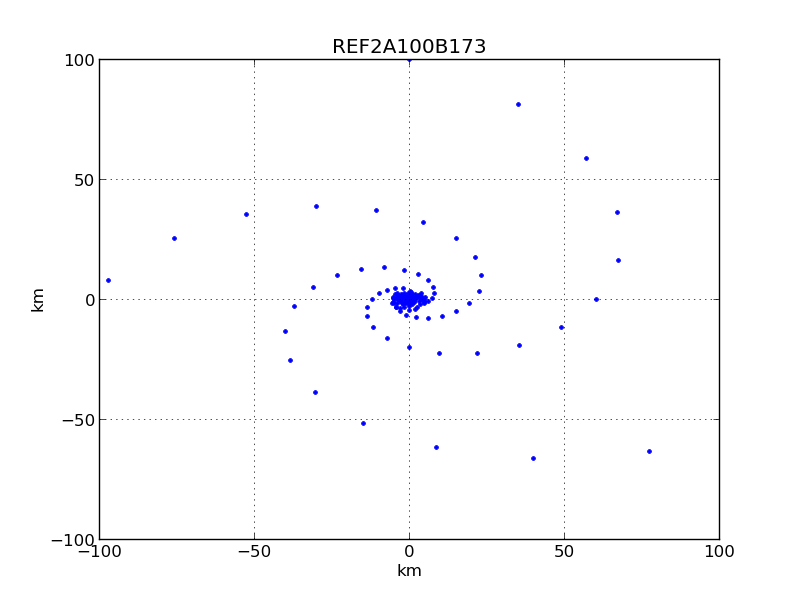
\includegraphics[width=0.180000\textwidth,trim= 0 .05cm 0 0.05cm]{{images/lay_SKA1REF2}.png} &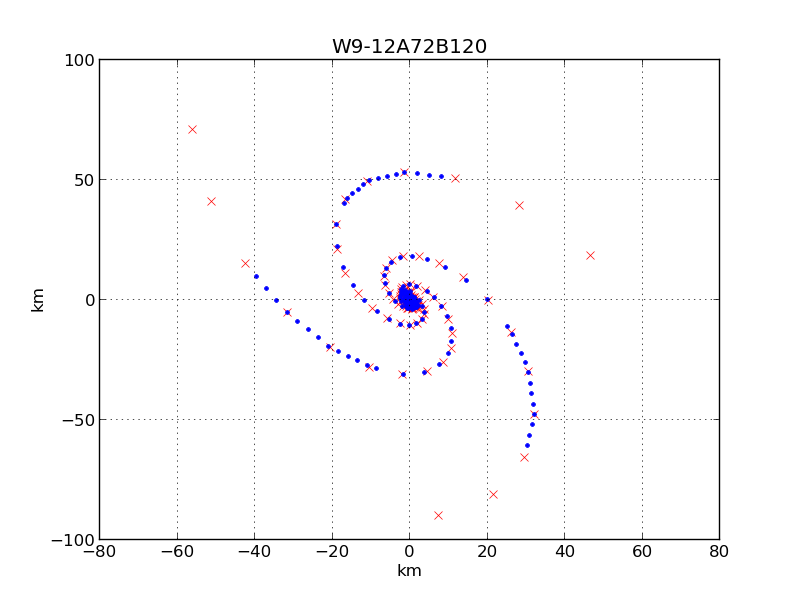
\includegraphics[width=0.180000\textwidth,trim= 0 .05cm 0 0.05cm]{{images/lay_SKA1W9-12A72B120}.png} &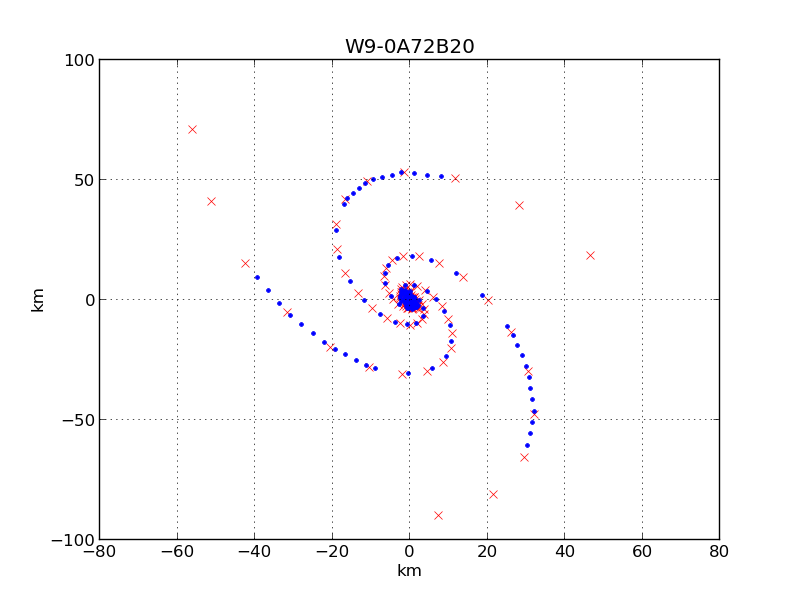
\includegraphics[width=0.180000\textwidth,trim= 0 .05cm 0 0.05cm]{{images/lay_SKA1W9-0A72B120}.png} &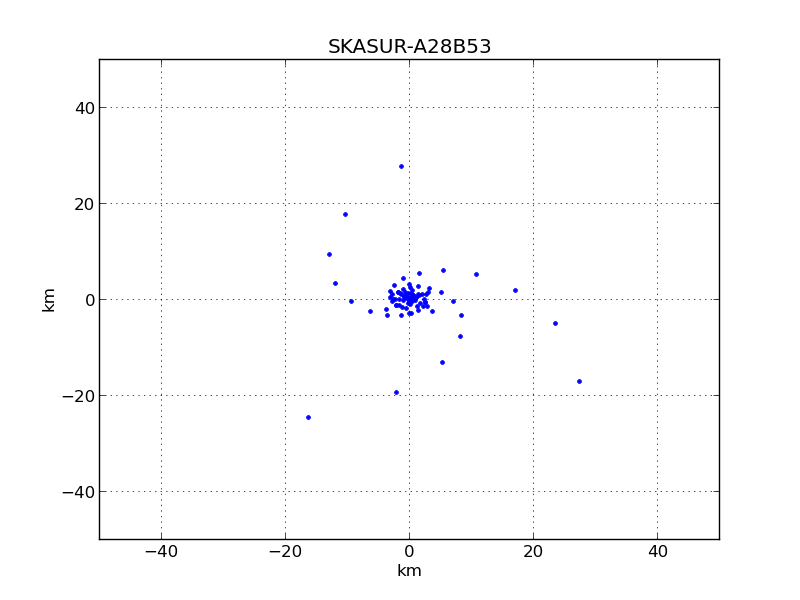
\includegraphics[width=0.180000\textwidth,trim= 0 .05cm 0 0.05cm]{{images/lay_SKASUR1}.png} &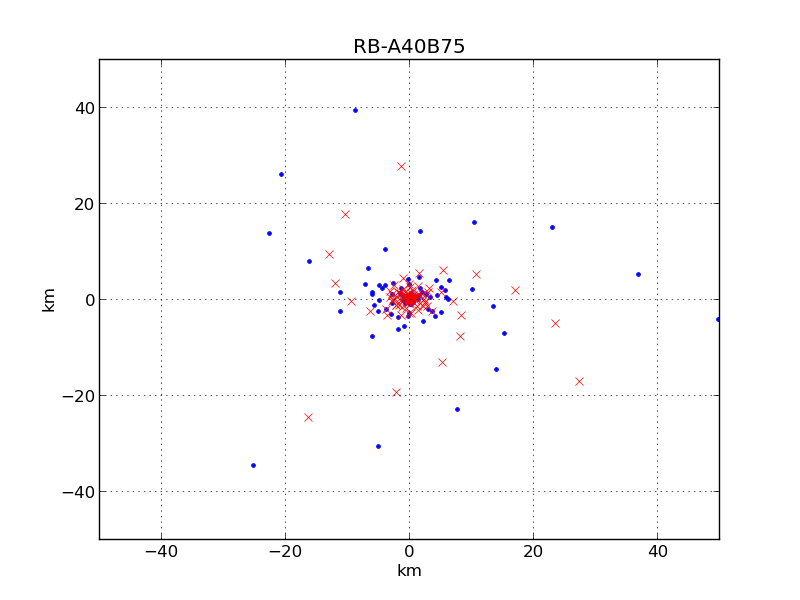
\includegraphics[width=0.180000\textwidth,trim= 0 .05cm 0 0.05cm]{{images/lay_SKASUR}.png} 
 \\ \hfill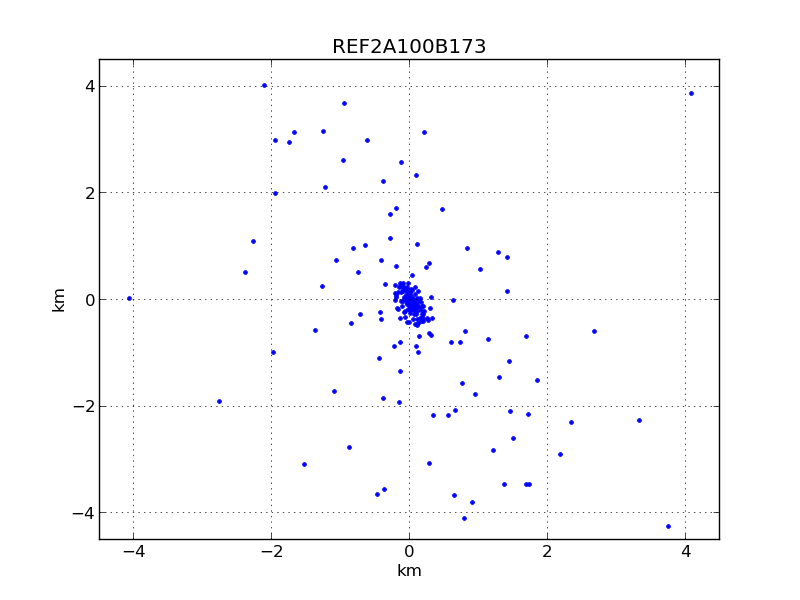
\includegraphics[width=0.180000\textwidth,trim= 0 .05cm 0 0.05cm]{{images/outer_core_SKA1REF2}.png} &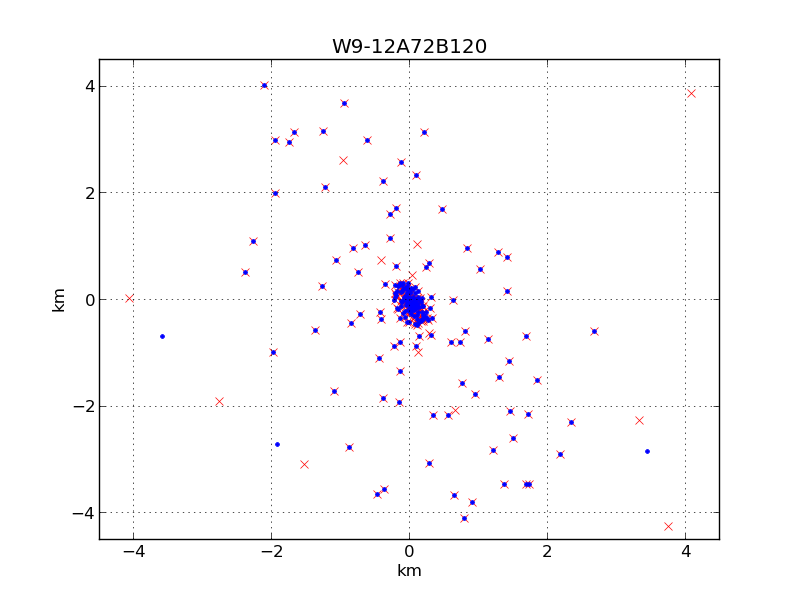
\includegraphics[width=0.180000\textwidth,trim= 0 .05cm 0 0.05cm]{{images/outer_core_SKA1W9-12A72B120}.png} &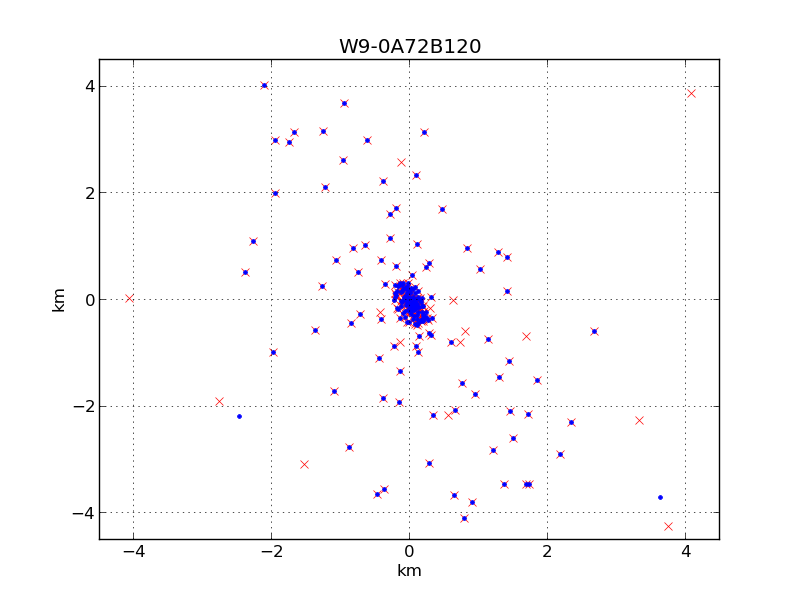
\includegraphics[width=0.180000\textwidth,trim= 0 .05cm 0 0.05cm]{{images/outer_core_SKA1W9-0A72B120}.png} &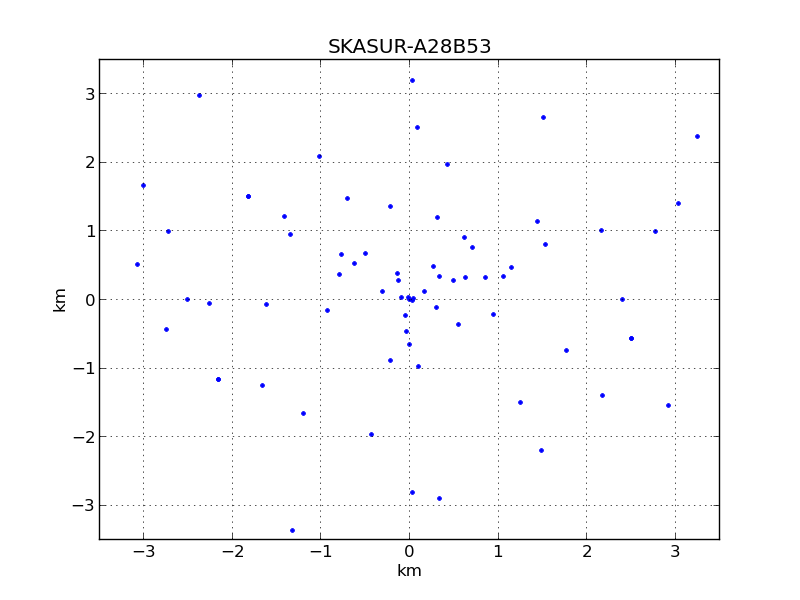
\includegraphics[width=0.180000\textwidth,trim= 0 .05cm 0 0.05cm]{{images/outer_core_SKASUR1}.png} &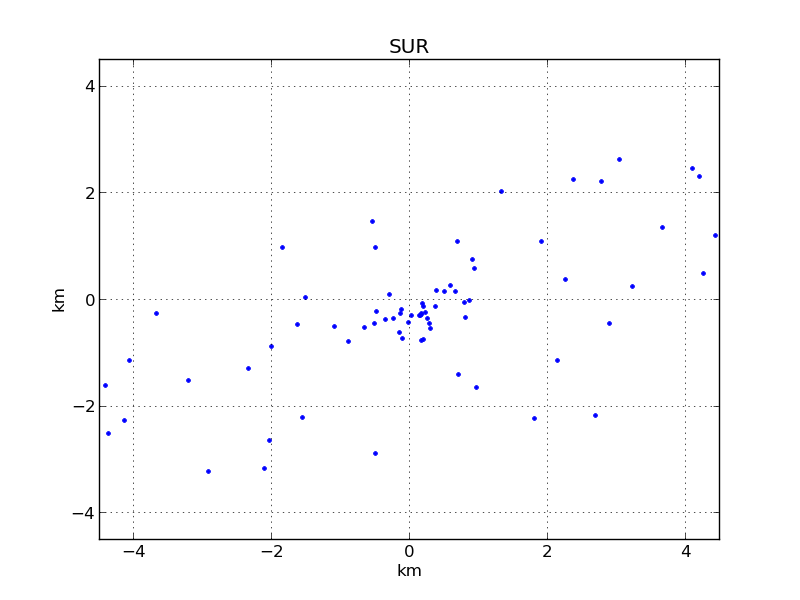
\includegraphics[width=0.180000\textwidth,trim= 0 .05cm 0 0.05cm]{{images/outer_core_SKASUR}.png} 
 \\ \hfill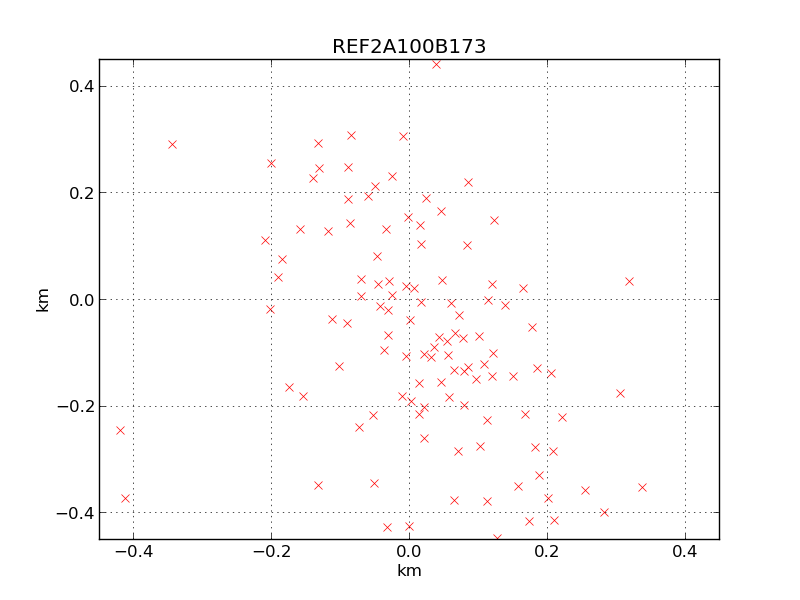
\includegraphics[width=0.180000\textwidth,trim= 0 .05cm 0 0.05cm]{{images/core_SKA1REF2}.png}
&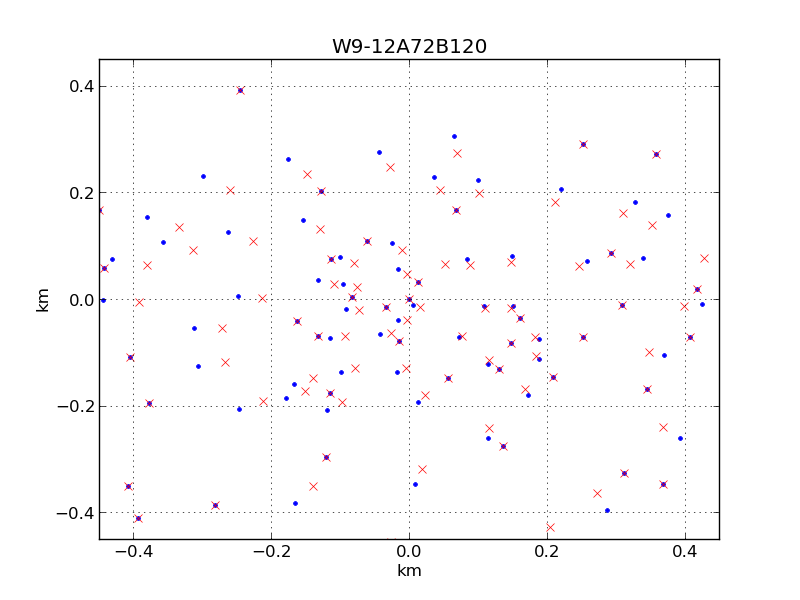
\includegraphics[width=0.180000\textwidth,trim= 0 .05cm 0 0.05cm]{{images/core_SKA1W9-12A72B120}.png}
&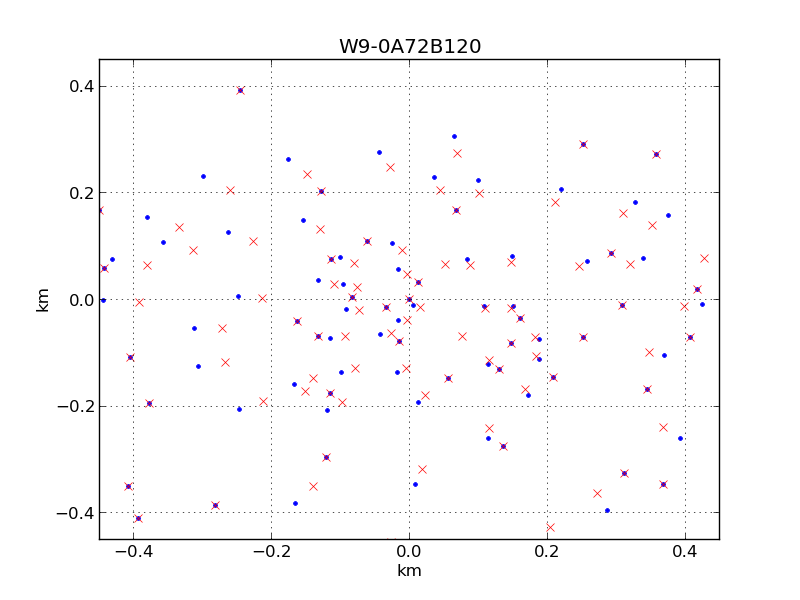
\includegraphics[width=0.180000\textwidth,trim= 0 .05cm 0 0.05cm]{{images/core_SKA1W9-0A72B120}.png}
& 
&  \\ \hfill\end{tabular}}
 \caption{Antenna layouts, V8 plotted as a reference (red crosses) for SKA1-MID layouts, and SUR
plotted as reference for the SUR75 layout. The vertical lines separate SKA1-MID and SKA
survey layouts.}\label{fig:lay}
\end{figure}
% baseline distribution histograms
\begin{figure}[H]
 \tiny{%%% autogen
 \begin{tabular}{llll||ll}
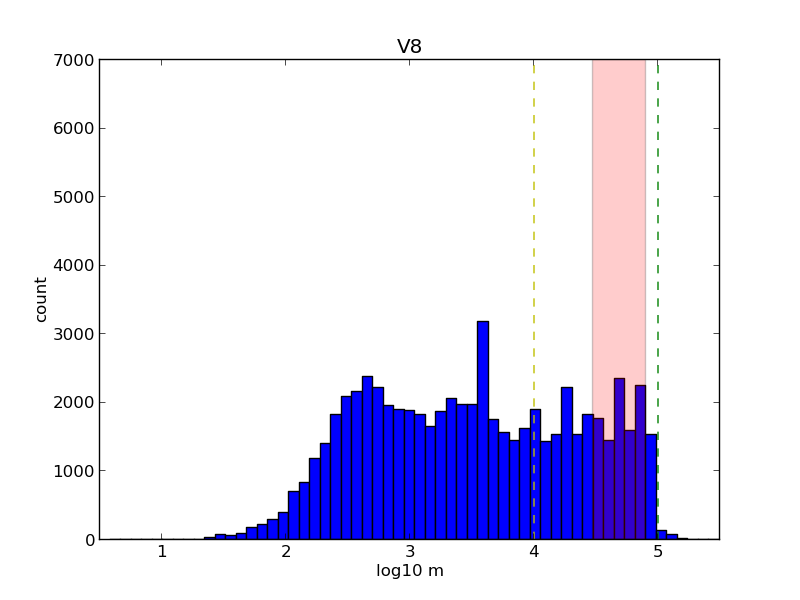
\includegraphics[width=0.150000\textwidth,trim= 0 .05cm 0 0.05cm]{{images/hist_SKA1V8}.png} &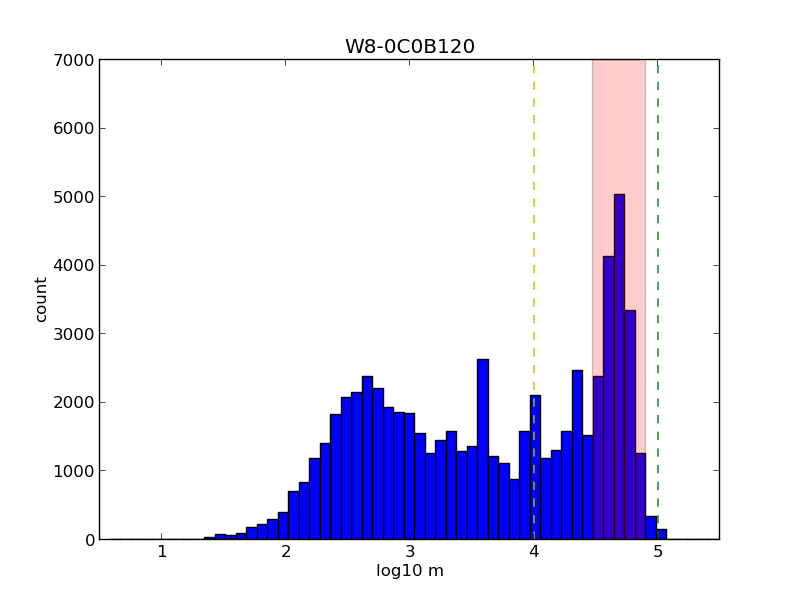
\includegraphics[width=0.150000\textwidth,trim= 0 .05cm 0 0.05cm]{{images/hist_SKA1W8-0C0B120}.png} &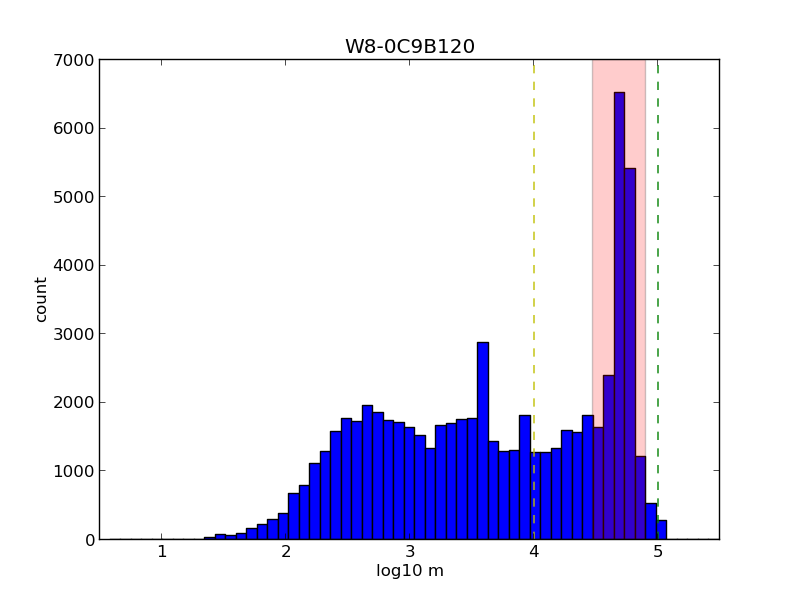
\includegraphics[width=0.150000\textwidth,trim= 0 .05cm 0 0.05cm]{{images/hist_SKA1W8-0C9B120}.png} &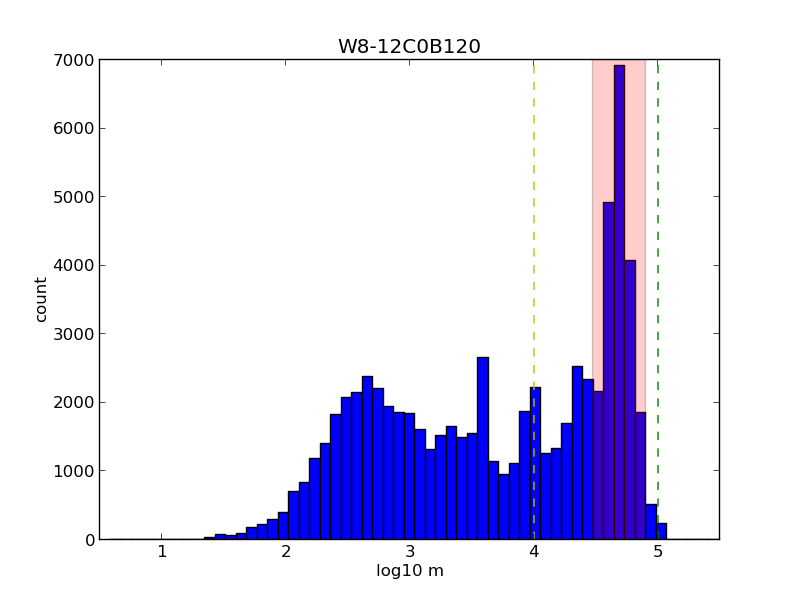
\includegraphics[width=0.150000\textwidth,trim= 0 .05cm 0 0.05cm]{{images/hist_SKA1W8-12C0B120}.png} &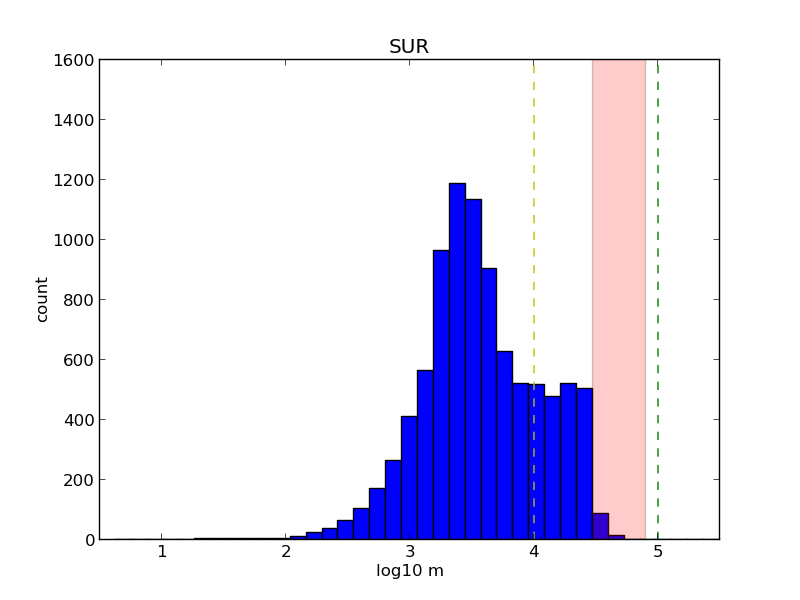
\includegraphics[width=0.150000\textwidth,trim= 0 .05cm 0 0.05cm]{{images/hist_SKASUR}.png} &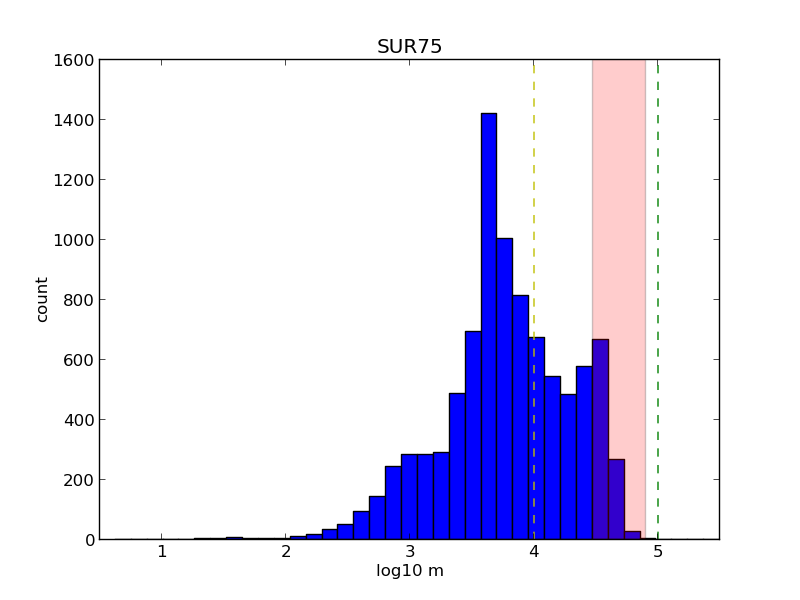
\includegraphics[width=0.150000\textwidth,trim= 0 .05cm 0 0.05cm]{{images/hist_SKASUR75}.png} 
 \\ \hfill\end{tabular}}
 \caption{Baseline distribution with the uv-distance in $log_{10}$ km . Yellow and green dashed lines mark 10 and 100
kilometres respectively, and the pink strip represents baselines from 30-80km.}\label{fig:hist}
\end{figure}
% \begin{figure}[H]
%  \centering
%  %%% autogen
 \begin{tabular}{ccc}
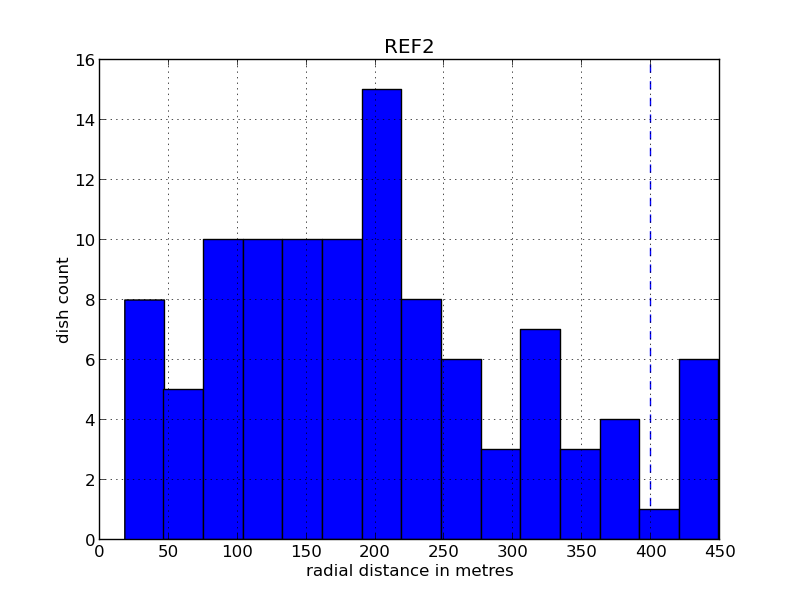
\includegraphics[width=0.300000\textwidth,trim= 0 .05cm 0 0.05cm]{{images/dish_hist-REF2}.png} &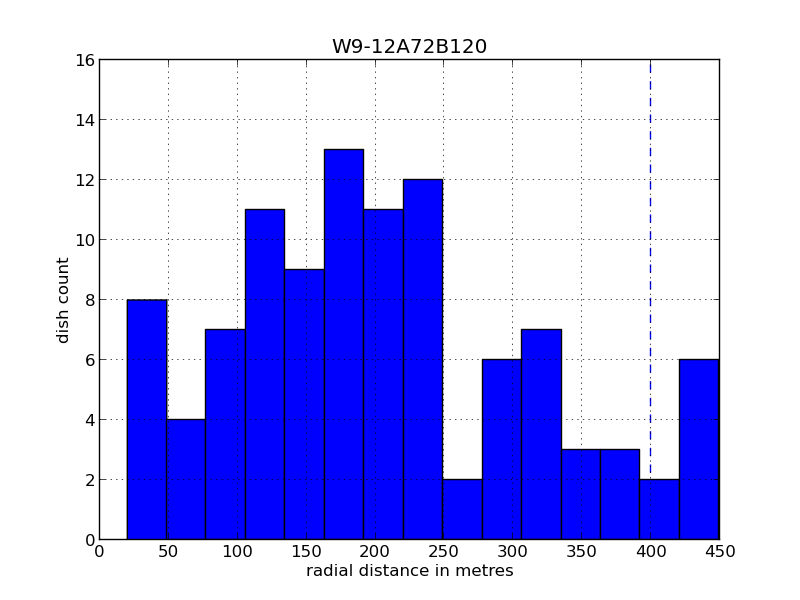
\includegraphics[width=0.300000\textwidth,trim= 0 .05cm 0 0.05cm]{{images/dish_hist-W9-12A72B120}.png} & 
 \\ \end{tabular}
%  \caption{Dish density histograms of the core of the SKA1-MID layouts under consideration. The dashed line marks 400m. The core
% of the W-9-j layouts is the same, therefore we only need to plot one of these.}
% \end{figure}
% \begin{figure}[H]
%  \centering
%  %%% autogen
 \begin{tabular}{ccc}
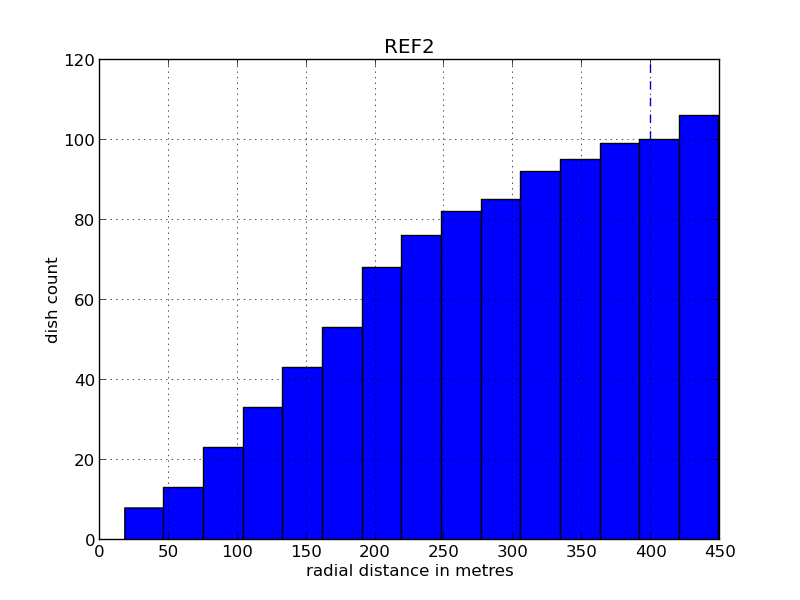
\includegraphics[width=0.300000\textwidth,trim= 0 .05cm 0 0.05cm]{{images/dish_cumhist-REF2}.png} &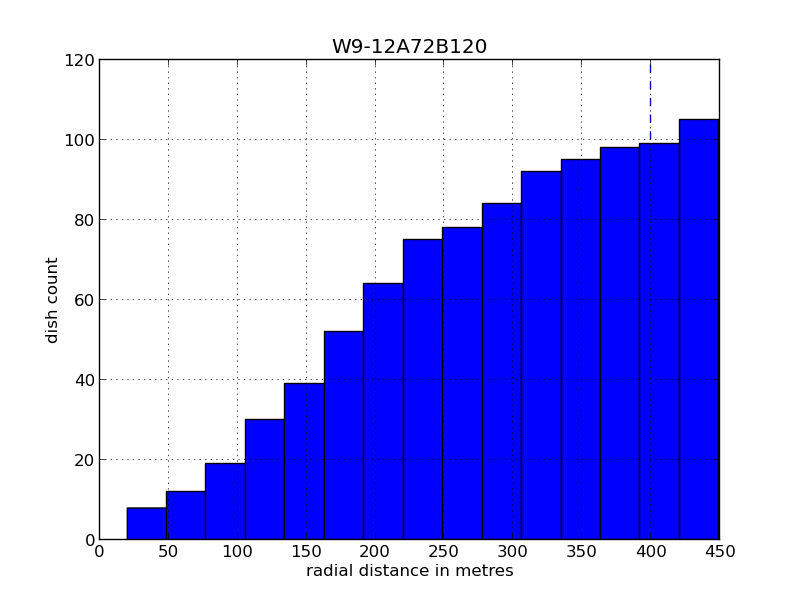
\includegraphics[width=0.300000\textwidth,trim= 0 .05cm 0 0.05cm]{{images/dish_cumhist-W9-12A72B120}.png} & 
 \\ \end{tabular}
%  \caption{Cumulative dish density histograms of the core of the SKA1-MID layouts under consideration. The dashed line marks 400m.
% The core of the W-9-j layouts is the same, therefore we only need to plot one of these.}
% \end{figure}
% uv-coverage plots 
\begin{figure}[H]
 \tiny{%%% autogen
 \begin{tabular}{llll||ll}
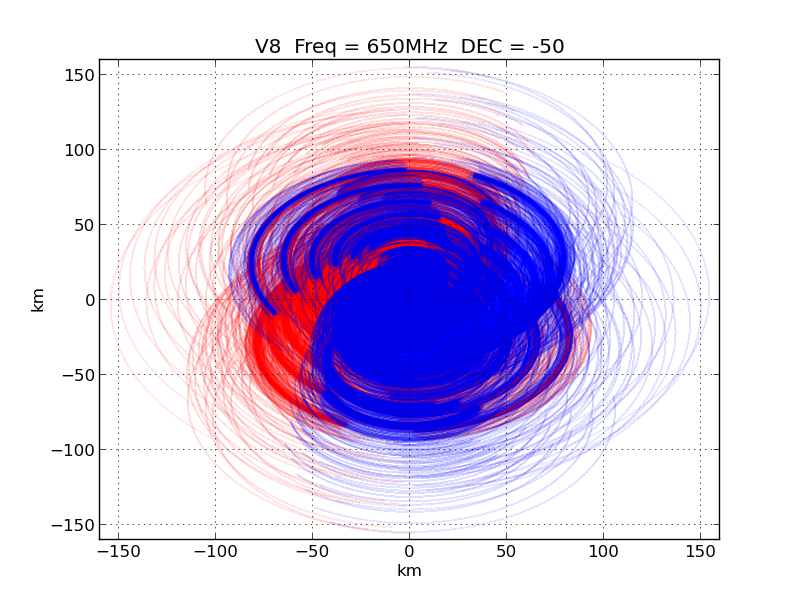
\includegraphics[width=0.150000\textwidth,trim= 0 .05cm 0 0.05cm]{{images/uvcov_-50SKA1V8}.png} &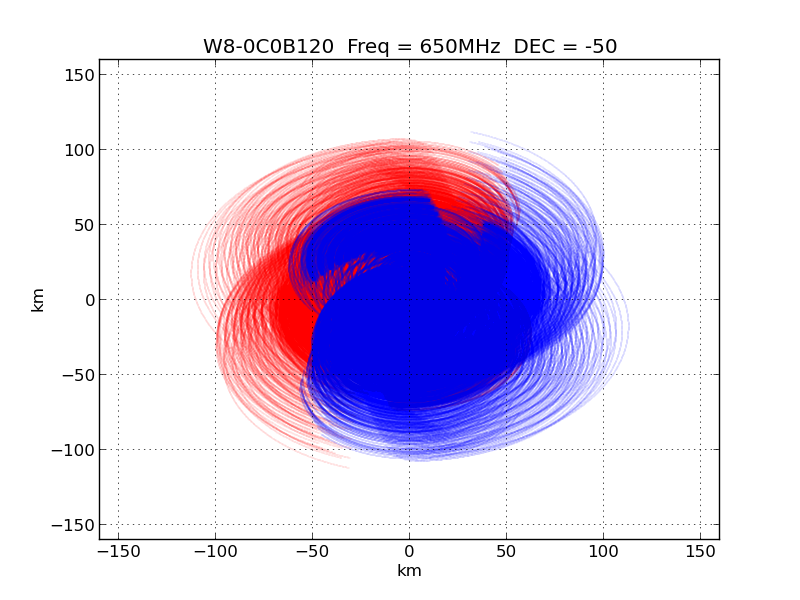
\includegraphics[width=0.150000\textwidth,trim= 0 .05cm 0 0.05cm]{{images/uvcov_-50SKA1W8-0C0B120}.png} &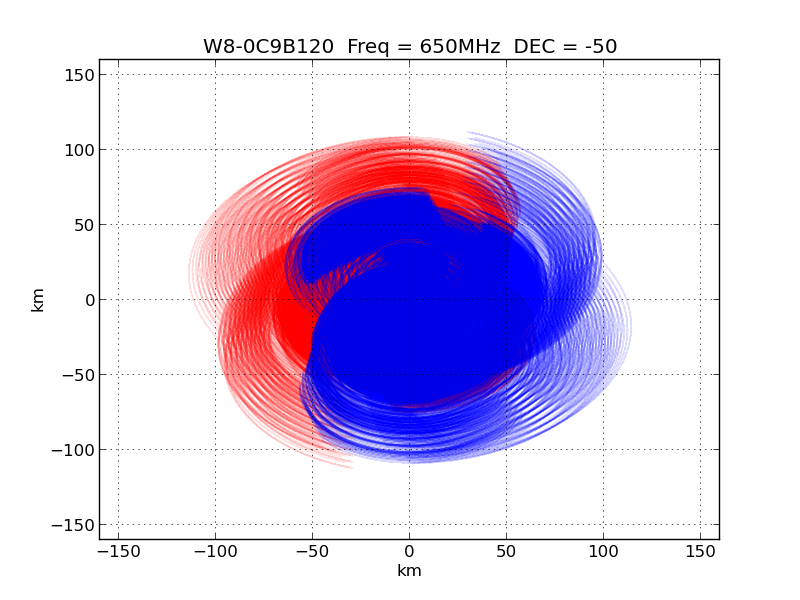
\includegraphics[width=0.150000\textwidth,trim= 0 .05cm 0 0.05cm]{{images/uvcov_-50SKA1W8-0C9B120}.png} &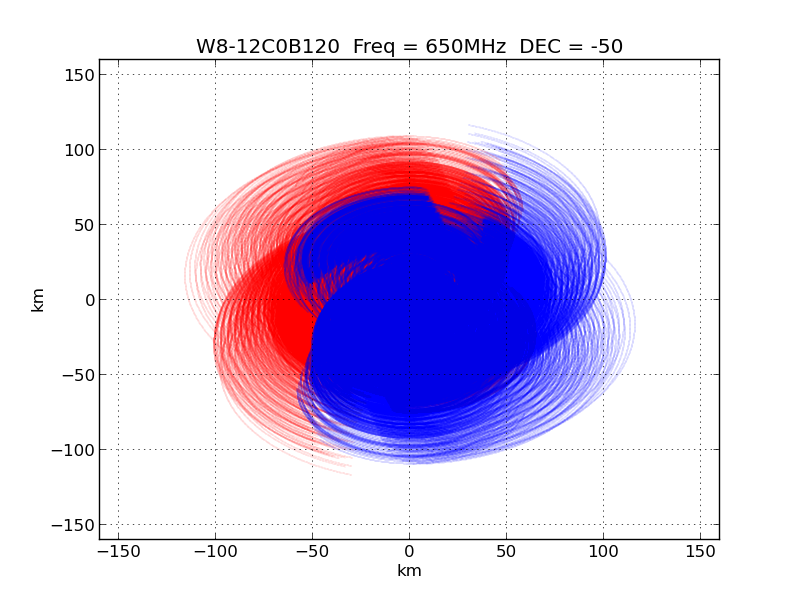
\includegraphics[width=0.150000\textwidth,trim= 0 .05cm 0 0.05cm]{{images/uvcov_-50SKA1W8-12C0B120}.png} &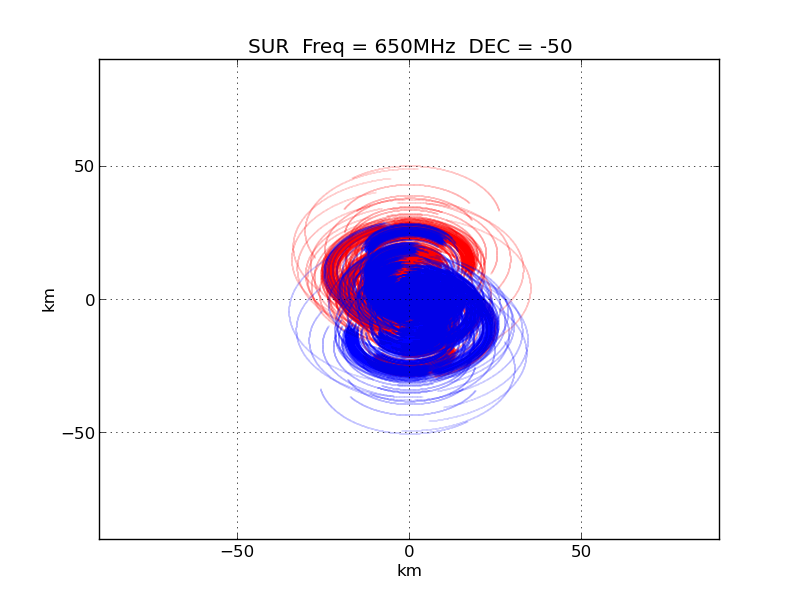
\includegraphics[width=0.150000\textwidth,trim= 0 .05cm 0 0.05cm]{{images/uvcov_-50SKASUR}.png} &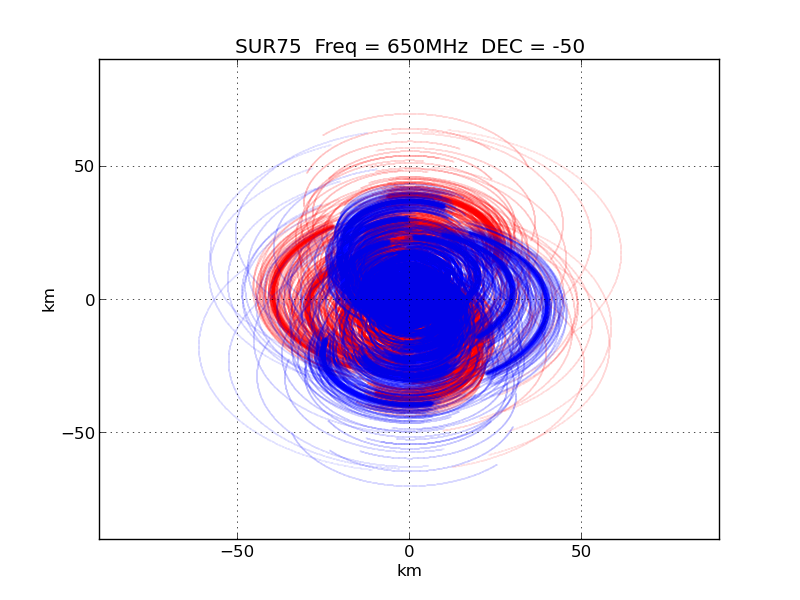
\includegraphics[width=0.150000\textwidth,trim= 0 .05cm 0 0.05cm]{{images/uvcov_-50SKASUR75}.png} 
 \\ \hfill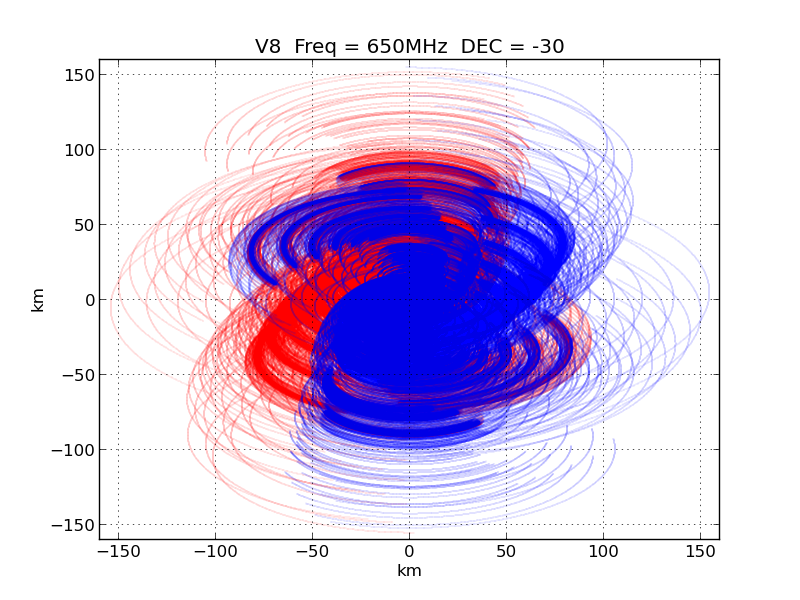
\includegraphics[width=0.150000\textwidth,trim= 0 .05cm 0 0.05cm]{{images/uvcov_-30SKA1V8}.png} &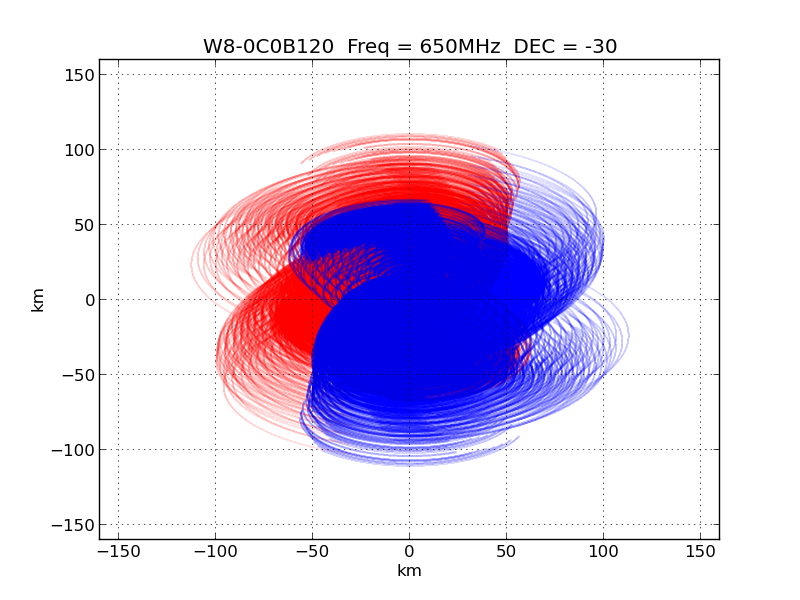
\includegraphics[width=0.150000\textwidth,trim= 0 .05cm 0 0.05cm]{{images/uvcov_-30SKA1W8-0C0B120}.png} &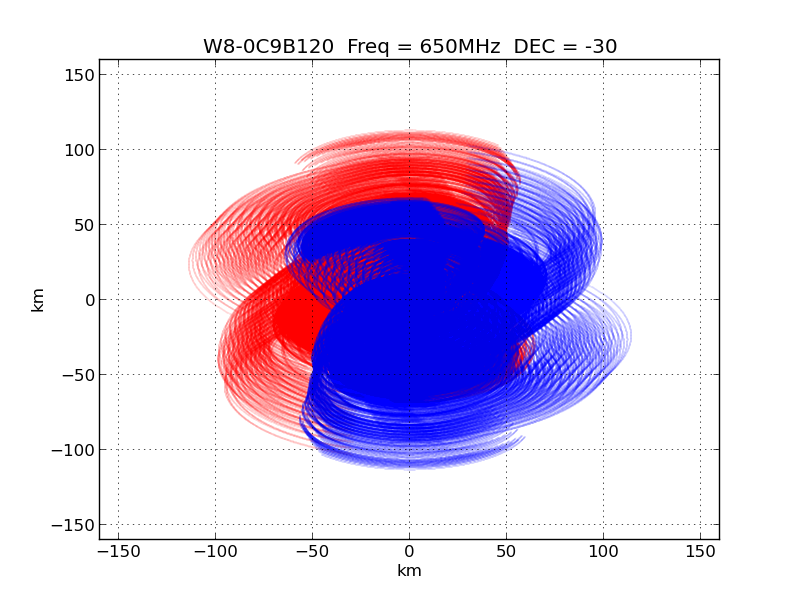
\includegraphics[width=0.150000\textwidth,trim= 0 .05cm 0 0.05cm]{{images/uvcov_-30SKA1W8-0C9B120}.png} &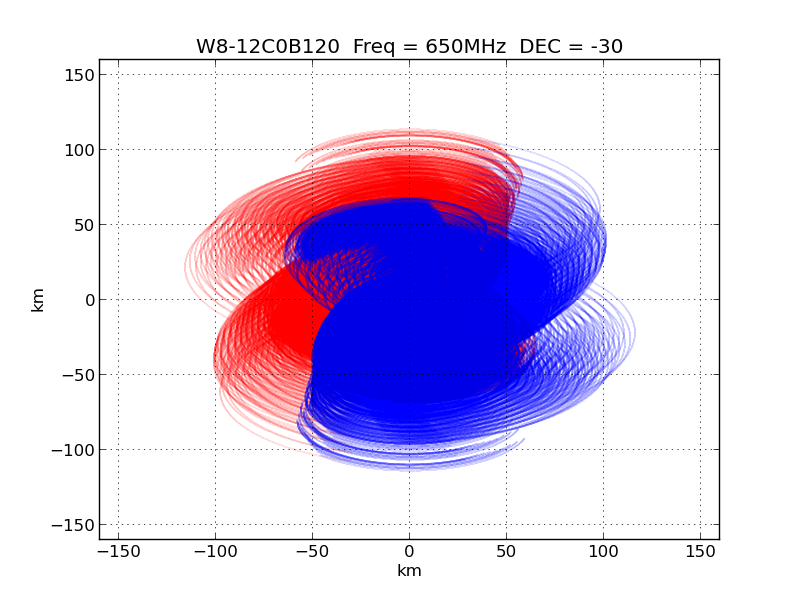
\includegraphics[width=0.150000\textwidth,trim= 0 .05cm 0 0.05cm]{{images/uvcov_-30SKA1W8-12C0B120}.png} &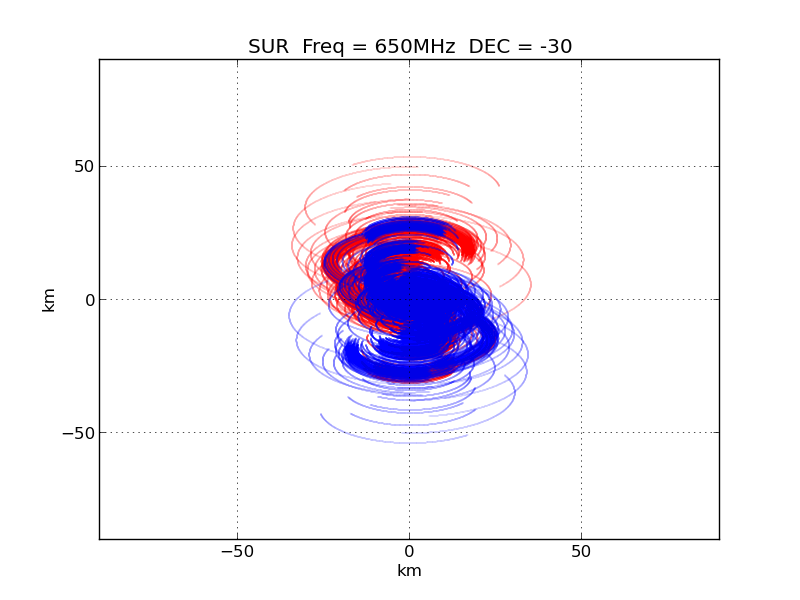
\includegraphics[width=0.150000\textwidth,trim= 0 .05cm 0 0.05cm]{{images/uvcov_-30SKASUR}.png} &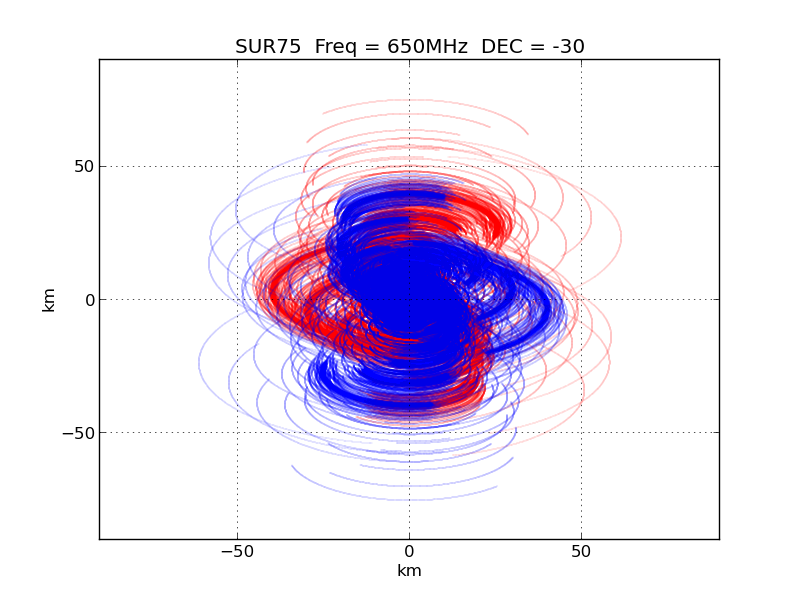
\includegraphics[width=0.150000\textwidth,trim= 0 .05cm 0 0.05cm]{{images/uvcov_-30SKASUR75}.png} 
 \\ \hfill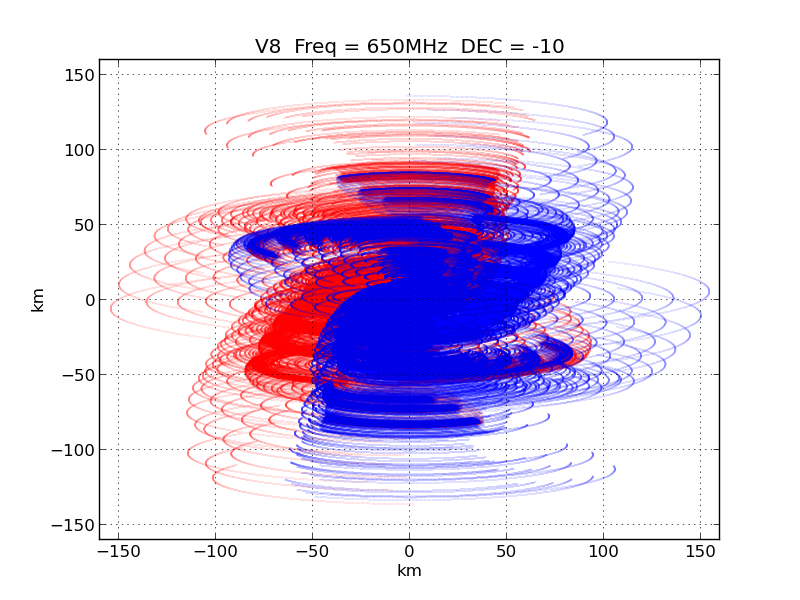
\includegraphics[width=0.150000\textwidth,trim= 0 .05cm 0 0.05cm]{{images/uvcov_-10SKA1V8}.png} &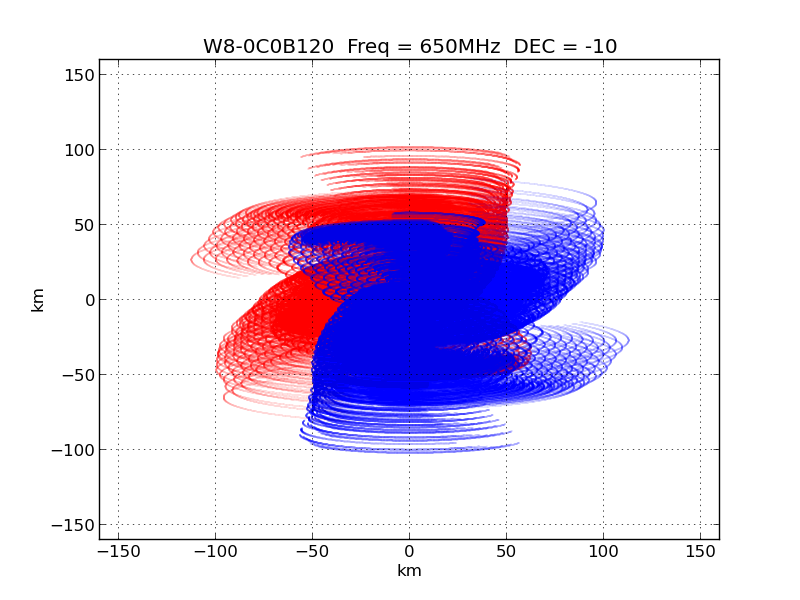
\includegraphics[width=0.150000\textwidth,trim= 0 .05cm 0 0.05cm]{{images/uvcov_-10SKA1W8-0C0B120}.png} &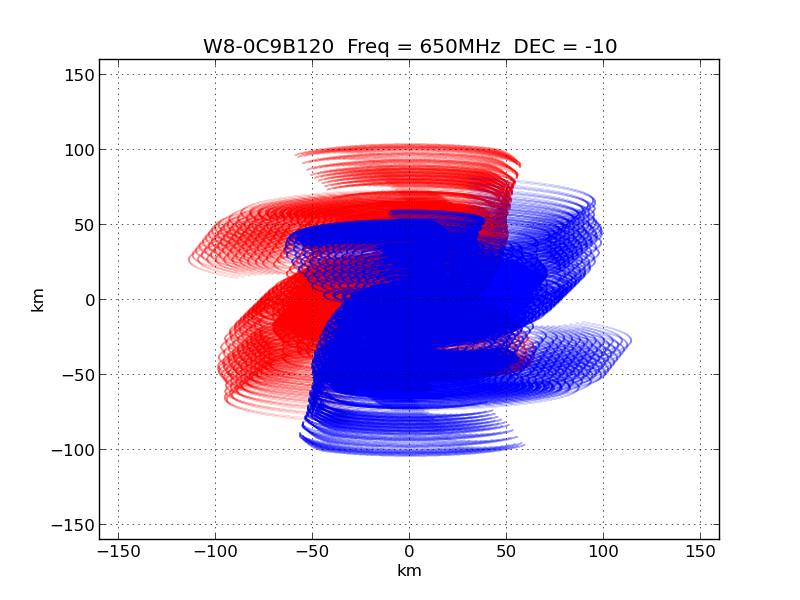
\includegraphics[width=0.150000\textwidth,trim= 0 .05cm 0 0.05cm]{{images/uvcov_-10SKA1W8-0C9B120}.png} &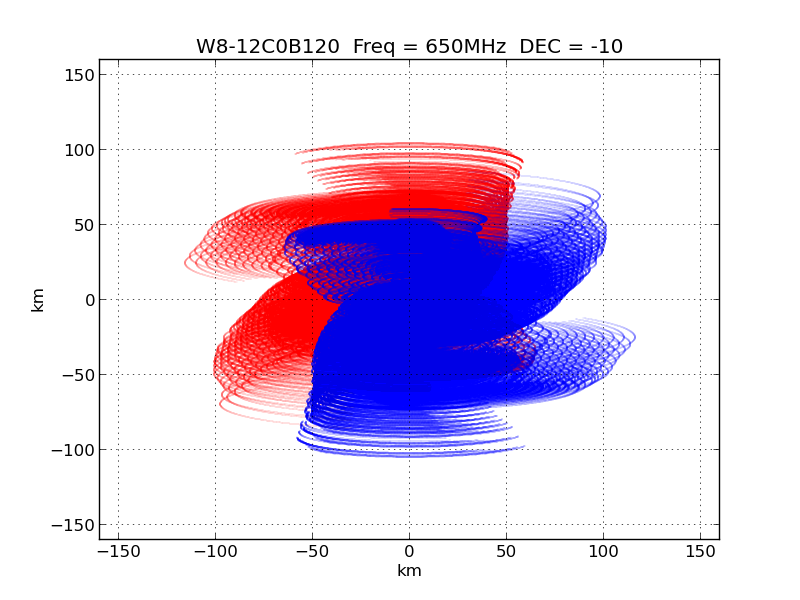
\includegraphics[width=0.150000\textwidth,trim= 0 .05cm 0 0.05cm]{{images/uvcov_-10SKA1W8-12C0B120}.png} &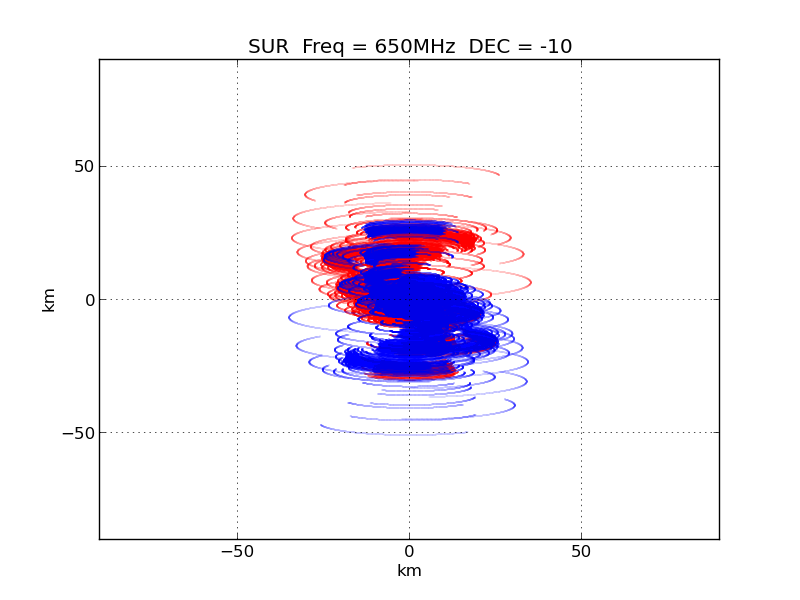
\includegraphics[width=0.150000\textwidth,trim= 0 .05cm 0 0.05cm]{{images/uvcov_-10SKASUR}.png} &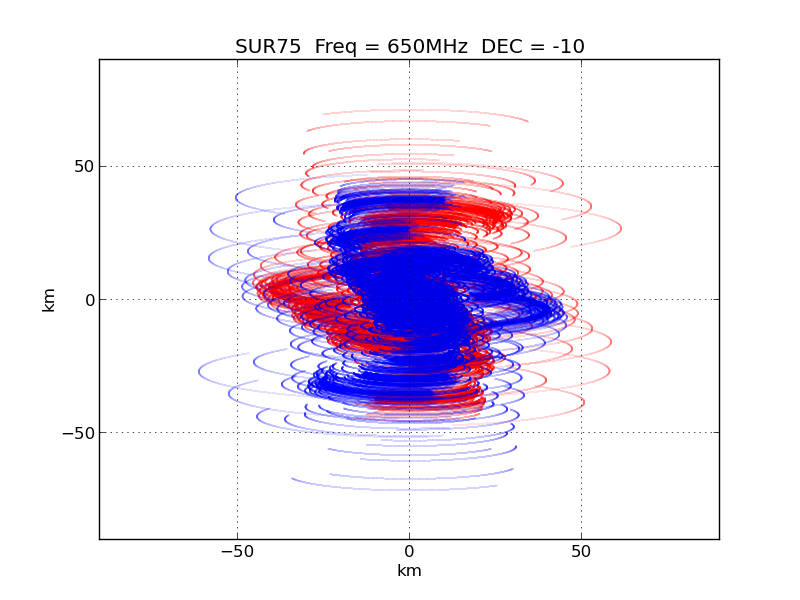
\includegraphics[width=0.150000\textwidth,trim= 0 .05cm 0 0.05cm]{{images/uvcov_-10SKASUR75}.png} 
 \\ \hfill\end{tabular}}
 \caption{UV-Coverage for 8-hr tracks at 650MHz (50MHz bandwidth) at declinations -50,-30,-10 for the different layouts. Blue
indicates uv-points, red indicates conjugate uv-points. The vertical lines separate SKA1-MID and SKA
survey layouts.}\label{fig:uvcov}
\end{figure}

\section{The Experiment}\label{sec:exp}
Our aim is to investigate the scale-dependent sensitivity of the layouts described in the previous section.
We use the \texttt{makems} tool to make simulated measurement sets (MS) of 8hr tracks with a 60s integration time for
declinations -50, -30 and -10 degrees, at frequencies of 650, 800, 1000 and 1400MHz, with a single 50MHz channel. The expected rms noise
per real and imaginary part for each visibility is calculated as 
\begin{equation}
\sigma_{\text{vis}} = \frac{\text{SEFD}}{\sqrt{2\Delta t\Delta \nu}}.
\end{equation}
We use the baseline design's SEFD values for the SKA and legacy dishes. The noise for visibilities corresponding to baselines
between SKA and legacy dishes is calculated using $\text{SEFD}_{\text{MIX}}=\sqrt{\text{SEFD}_{\text{SKA}} \times
\text{SEFD}_{\text{LEGACY}}}$. The MS is then filled with random Gaussian noise using the computed value of the noise for a
given integration and bandwidth. We then use the (CASA-derived) \texttt{lwimager} tool to make dirty maps of
the PSF as well as dirty maps of the noise using various weighting and tapering schemes. Note that for uniform and
robust weighting, a crucial parameter is the size of the uv-bin over which weights are “uniformized”. By default this is
determined from the full image size, but \texttt{lwimager} allows one to uniformize the weights over bins corresponding
to a user-defined FoV instead. For these simulations uv-bins corresponding to a FoV of 10 arcmin were used. The
following metrics were generated:
\begin{itemize}
 \item PSF full width at half maximum (FWHM) size (mean of the FWHM dimensions). This was measured by making high-resolution
images of the PSF (0.05 arcsec resolution), and fitting a Gaussian to the PSF (Table \ref{tab:psf_mean-dec30}). A
catalog
of PSF
cross-sections (full uv-coverage) is provided in Appendix \ref{app:psf}.

 \item PSF symmetry (PSF size parameters are obtained as explained above). As a measure of PSF symmetry, we define 
$\text{PSF}_{sym}=1-\text{FWHM}_{min}/\text{FWHM}_{maj}$, then $\text{PSF}_{sym} = 0$ is perfect symmetry, and the symmetry
degenerates as $\text{PSF}_{sym}\,\,\, \rightarrow\,\,1$ (Table \ref{tab:psf_sym-dec30}).

 \item RMS pixel noise at different angular scales for 50kHz, 50MHz and 166MHz wide bands (Tables
\ref{tab:noise50k-dec30} -
\ref{tab:noise166-dec30}).

\item RMS PSF far sidelobe level. These were measured by making images of the PSF 1 degree across, and measuring
the rms levels beyond a radius of 30 arcmin.

 \item SNR for a 10$\mu$Jy source at 1000MHz with a spectral index of -0.7 after 8hrs for a 166MHz band (Table
\ref{tab:snr10-dec30}).
 
 \item Average SNR over frequencies 650, 800 and 1000MHz (166MHz band) after 8 hours, for a 10$\mu$Jy source at 1000MHz
with a
spectral index of -0.7. {$\overline{\text{SNR10}}=\sqrt{\frac{1}{3}(\text{SNR10}_{650}^2 + \text{SNR10}_{800}^2
+\text{SNR10}_{1000}^2})$} (Table \ref{tab:snravg-dec30}).

 \item Hours required to reach a mean SNR of 10 (Table \ref{tab:hours-dec30}).
 
 \item Survey Speed. These values are calculated using the FOV values in the SRD (band 1 for SKA1-MID and band 2 PAF FOV
for
SKASUR) and the values in Table \ref{tab:snr10-dec30}. Note that unlike the SKASUR FOV, the SKA1-MID FOV changes across
the band
(FOV$_{\text{Mid}}\sim \nu^{-2}$). $\text{SS}_\text{Freq} = \text{FOV}_\text{Freq}\times \text{SNR}^2$. 
% We consider band 1 for SKA-MID and band 2 for SKASUR. 
 \item Average survey speed. {$\overline{\text{SS}} =\sqrt{\frac{1}{3}(\text{SS}_{650}^2 + \text{SS}_{800}^2
+\text{SS}_{1000}^2})$} (Table \ref{tab:speed_avg-dec30}).
\end{itemize}
% \newpage
\section{Simulation Results}\label{sec:results}
\subsection{PSF and Noise Statistics}
% In appendix \ref{sec:band5} the above mentioned metrics are presented for a 2.5GHz band at 8, 12 and 13.8GHz, at a
% declination of -30 degrees.
Figure \ref{fig:full-psf_meam} shows the PSF sizes (FWHM) for the layouts under consideration as a function of frequency
for natural and robust-2 weighting as well as robust-2 weighting  with a 1$''$ Gaussian taper at a declination of -30
degrees. Note that for natural weighting the PSF is highly non-Gaussian (see appendix \ref{app:psf}) therefore the FWHM
size is not representative of the PSF size. The PSF sizes for the SKA1-MID layouts are similar for the other two
weighting schemes, while unsurprisingly, the SUR75 has a significantly smaller PSF compared to SUR. In the case of
SKA1-MID, this shows that a 120km maximum baseline layout has very similar resolving performance compared to a 150km
maximum baseline layout, given our optimizations for increased sensitivity at the longer baselines.

Figure~\ref{fig:full-psf_sym} shows a measure of the PSF symmetry for the different layouts. We note that our alternate 
layouts result in a less symmetric naturally-weighted PSF, but do not significantly change the uniformly-weighted PSF. 
Figures~\ref{fig:full-noise50} and \ref{fig:full-noise50k} show the expected rms noise, in $\mu$Jy/beam, as a function 
of frequency. Finally, Fig.~\ref{fig:full-sdl} shows the PSF far sidelobe level. We note that especially in the 
uniformly-weighted case, this is noticeably lower for our alternate layouts.

\begin{figure}[H]
%  %%% autogen
 \begin{tabular}{lll}
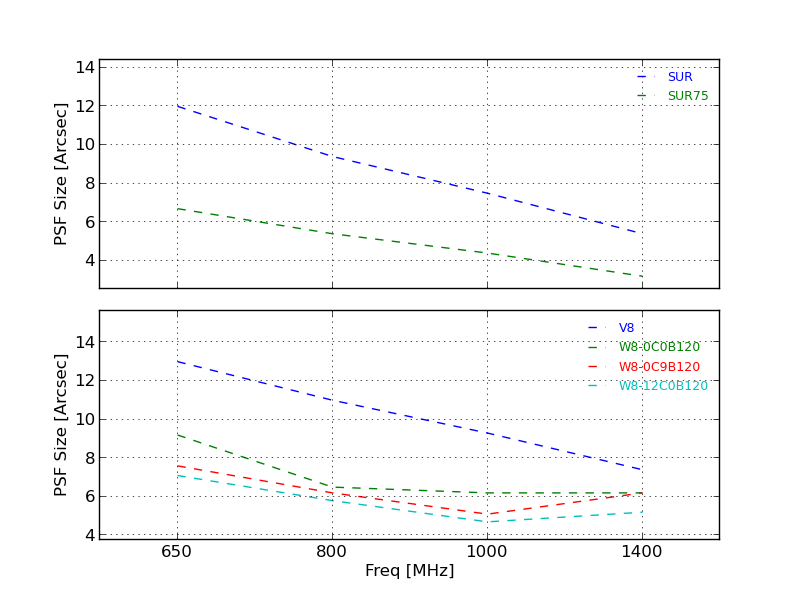
\includegraphics[width=0.300000\textwidth,trim= 0 .05cm 0 0.05cm]{{images/psf_mean-0_-10}.png} &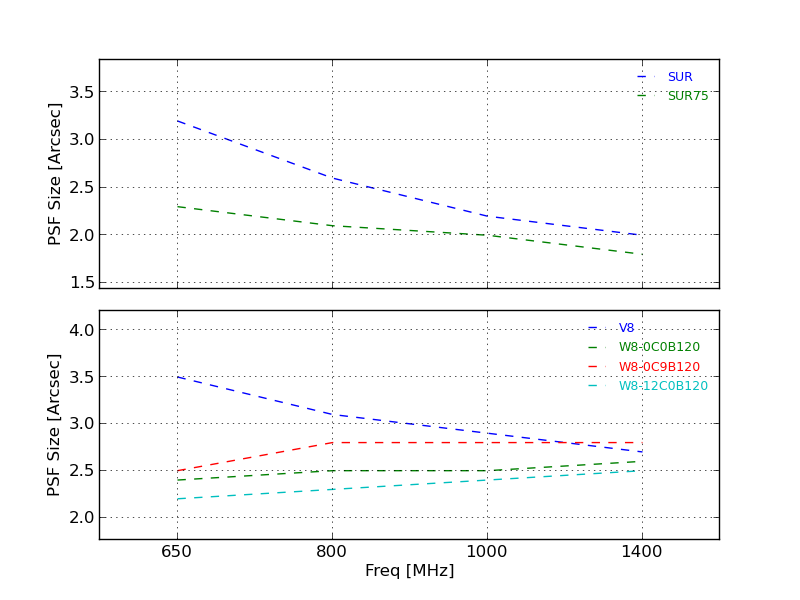
\includegraphics[width=0.300000\textwidth,trim= 0 .05cm 0 0.05cm]{{images/psf_mean-1_-10}.png} &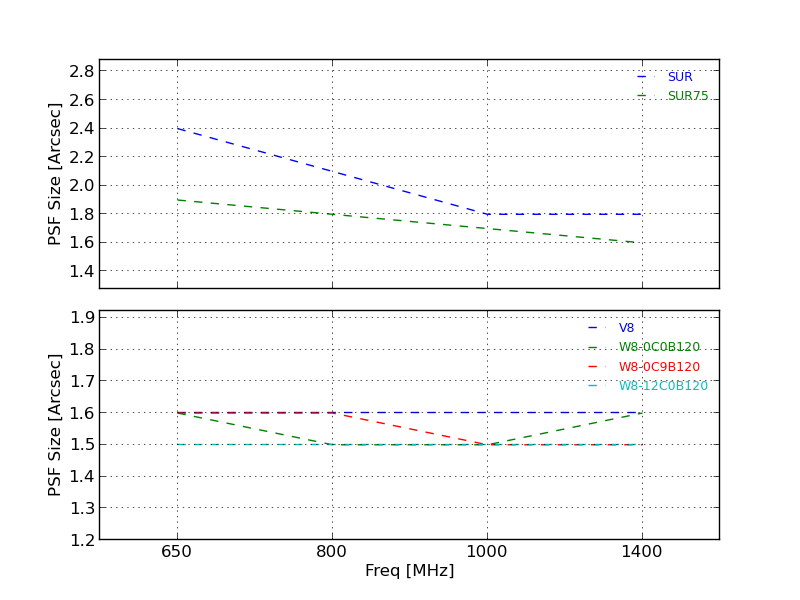
\includegraphics[width=0.300000\textwidth,trim= 0 .05cm 0 0.05cm]{{images/psf_mean-2_-10}.png} 
 \\ \hfill\end{tabular}
 %%% autogen
 \begin{tabular}{lll}
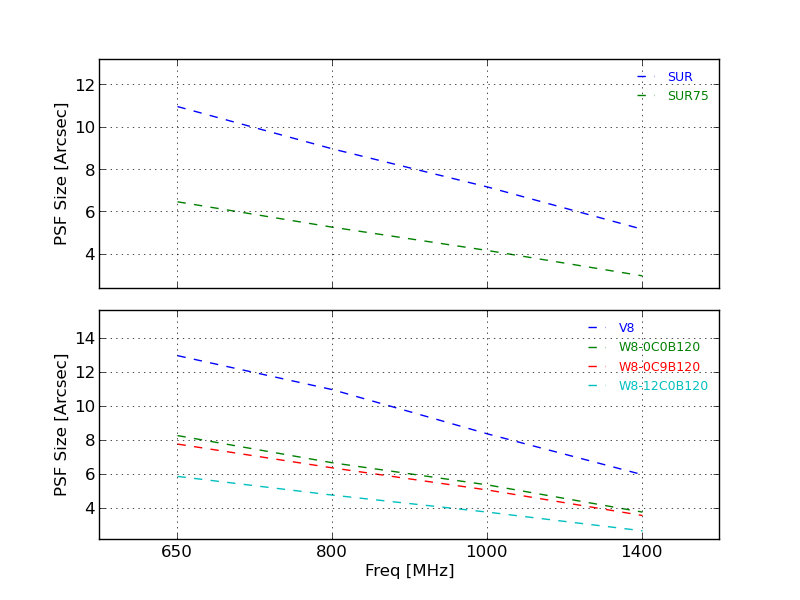
\includegraphics[width=0.300000\textwidth,trim= 0 .05cm 0 0.05cm]{{images/psf_mean-0_-30}.png} &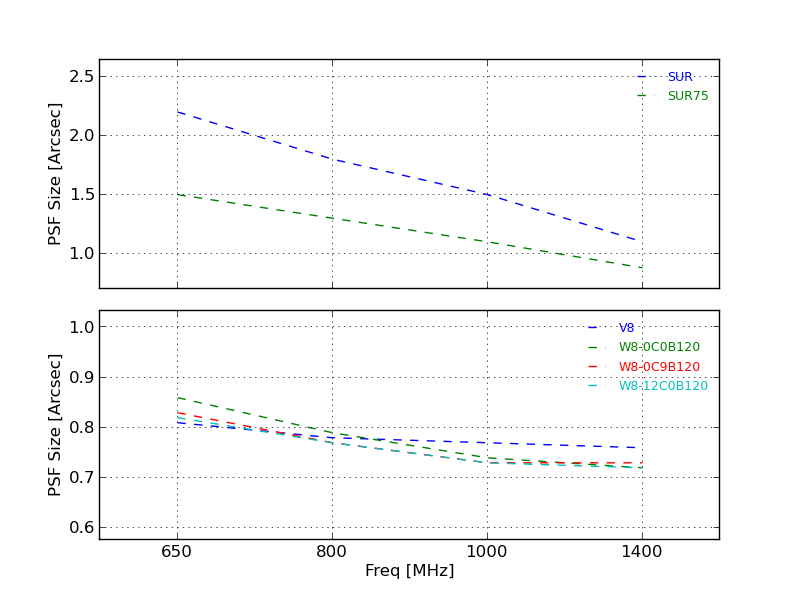
\includegraphics[width=0.300000\textwidth,trim= 0 .05cm 0 0.05cm]{{images/psf_mean-1_-30}.png} &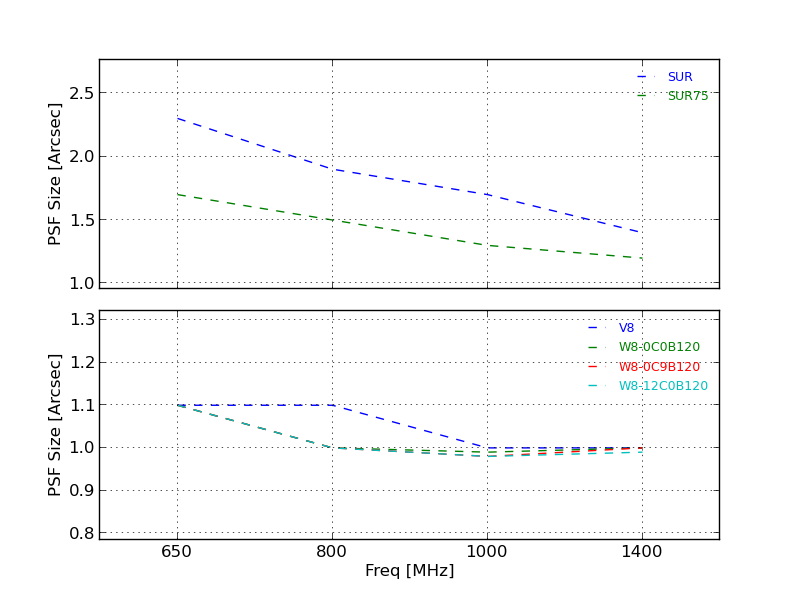
\includegraphics[width=0.300000\textwidth,trim= 0 .05cm 0 0.05cm]{{images/psf_mean-2_-30}.png} 
 \\ \hfill\end{tabular}
%  %%% autogen
 \begin{tabular}{lll}
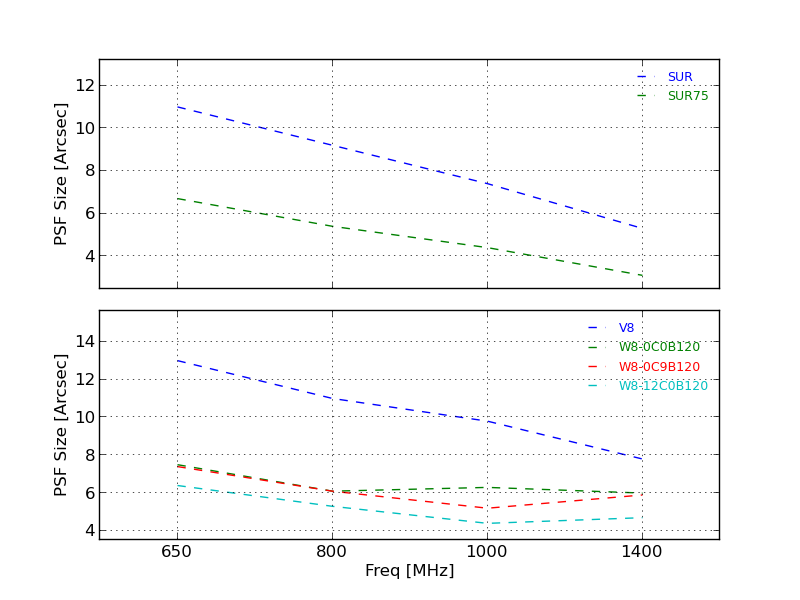
\includegraphics[width=0.300000\textwidth,trim= 0 .05cm 0 0.05cm]{{images/psf_mean-0_-50}.png} &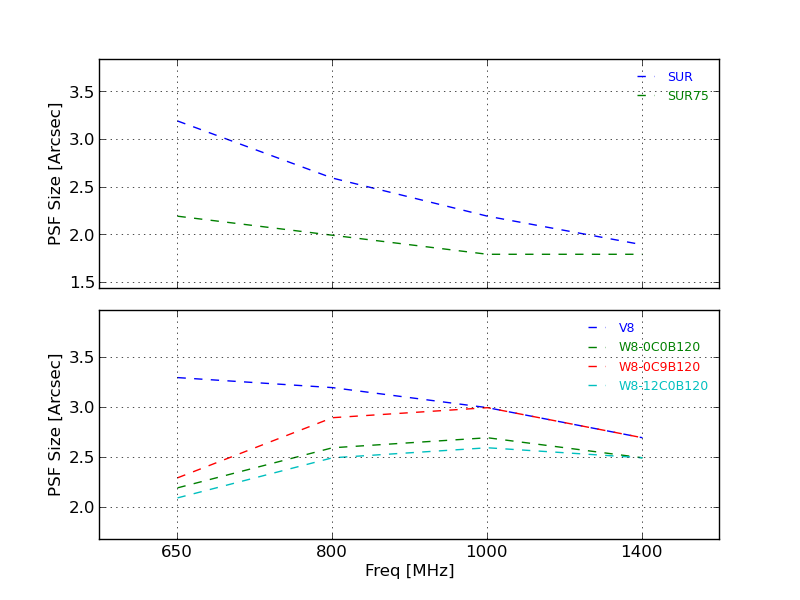
\includegraphics[width=0.300000\textwidth,trim= 0 .05cm 0 0.05cm]{{images/psf_mean-1_-50}.png} &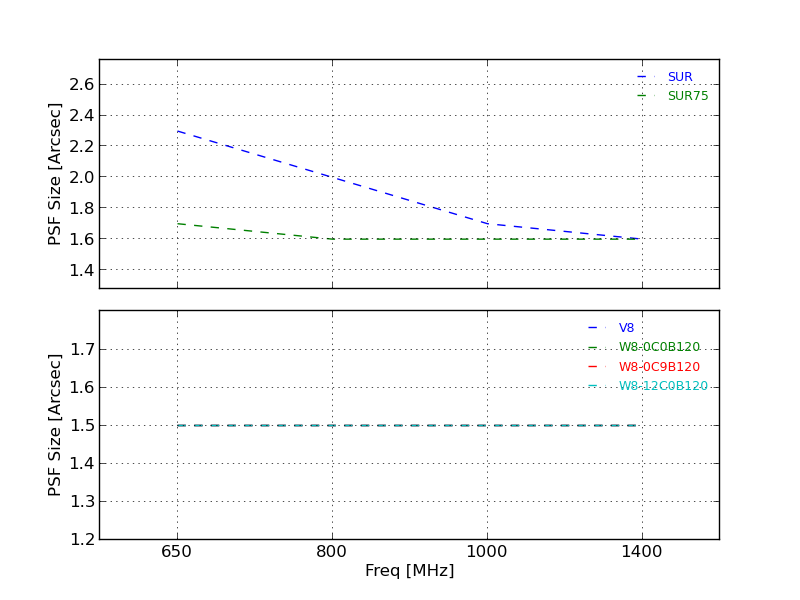
\includegraphics[width=0.300000\textwidth,trim= 0 .05cm 0 0.05cm]{{images/psf_mean-2_-50}.png} 
 \\ \hfill\end{tabular}
 \caption{PSF size as a function of frequency for the SKA survey layouts (top) and MID layouts (bottom).
This is done for natural (column 1) and robust-2 weighting (column 2) as well as robust-2 weighting  with a 1$''$
Gaussian taper (column 3) at a declination of -30 degrees.}\label{fig:full-psf_meam}
\end{figure}

\begin{figure}[H]
%  %%% autogen
 \begin{tabular}{lll}
\includegraphics[width=0.300000\textwidth,trim= 0 .05cm 0 0.05cm]{{images/psf_sym-0_-10}.png} &\includegraphics[width=0.300000\textwidth,trim= 0 .05cm 0 0.05cm]{{images/psf_sym-1_-10}.png} &\includegraphics[width=0.300000\textwidth,trim= 0 .05cm 0 0.05cm]{{images/psf_sym-2_-10}.png} 
 \\ \hfill\end{tabular}
 %%% autogen
 \begin{tabular}{lll}
\includegraphics[width=0.300000\textwidth,trim= 0 .05cm 0 0.05cm]{{images/psf_sym-0_-30}.png} &\includegraphics[width=0.300000\textwidth,trim= 0 .05cm 0 0.05cm]{{images/psf_sym-1_-30}.png} &\includegraphics[width=0.300000\textwidth,trim= 0 .05cm 0 0.05cm]{{images/psf_sym-2_-30}.png} 
 \\ \hfill\end{tabular}
%  %%% autogen
 \begin{tabular}{lll}
\includegraphics[width=0.300000\textwidth,trim= 0 .05cm 0 0.05cm]{{images/psf_sym-0_-50}.png} &\includegraphics[width=0.300000\textwidth,trim= 0 .05cm 0 0.05cm]{{images/psf_sym-1_-50}.png} &\includegraphics[width=0.300000\textwidth,trim= 0 .05cm 0 0.05cm]{{images/psf_sym-2_-50}.png} 
 \\ \hfill\end{tabular}
 \caption{PSF symmetry as a function of frequency for the SKA survey layouts (top) and MID layouts (bottom).
This is done for natural (column 1) and robust-2 weighting (column 2) as well as robust-2 weighting  with a 1$''$
Gaussian taper (column 3) at a declination of -30 degrees.}\label{fig:full-psf_sym}
\end{figure}

\begin{figure}[H]
%  %%% autogen
 \begin{tabular}{lll}
\includegraphics[width=0.300000\textwidth,trim= 0 .05cm 0 0.05cm]{{images/noise50-0_-10}.png} &\includegraphics[width=0.300000\textwidth,trim= 0 .05cm 0 0.05cm]{{images/noise50-1_-10}.png} &\includegraphics[width=0.300000\textwidth,trim= 0 .05cm 0 0.05cm]{{images/noise50-2_-10}.png} 
 \\ \hfill\end{tabular}
 %%% autogen
 \begin{tabular}{lll}
\includegraphics[width=0.300000\textwidth,trim= 0 .05cm 0 0.05cm]{{images/noise50-0_-30}.png} &\includegraphics[width=0.300000\textwidth,trim= 0 .05cm 0 0.05cm]{{images/noise50-1_-30}.png} &\includegraphics[width=0.300000\textwidth,trim= 0 .05cm 0 0.05cm]{{images/noise50-2_-30}.png} 
 \\ \hfill\end{tabular}
%  %%% autogen
 \begin{tabular}{lll}
\includegraphics[width=0.300000\textwidth,trim= 0 .05cm 0 0.05cm]{{images/noise50-0_-50}.png} &\includegraphics[width=0.300000\textwidth,trim= 0 .05cm 0 0.05cm]{{images/noise50-1_-50}.png} &\includegraphics[width=0.300000\textwidth,trim= 0 .05cm 0 0.05cm]{{images/noise50-2_-50}.png} 
 \\ \hfill\end{tabular}
 \caption{Noise for a 50MHz wide band and an 8 hour synthesis, as a function of frequency,
for the SKA survey layouts (top) and MID layouts (bottom).
This is done for natural (column 1) and robust-2 weighting (column 2) as well as robust-2 weighting  with a 1$''$
Gaussian taper (column 3) at a declination of -30 degrees.}\label{fig:full-noise50}
\end{figure}

\begin{figure}[H]
%  %%% autogen
 \begin{tabular}{lll}
\includegraphics[width=0.300000\textwidth,trim= 0 .05cm 0 0.05cm]{{images/noise50k-0_-10}.png} &\includegraphics[width=0.300000\textwidth,trim= 0 .05cm 0 0.05cm]{{images/noise50k-1_-10}.png} &\includegraphics[width=0.300000\textwidth,trim= 0 .05cm 0 0.05cm]{{images/noise50k-2_-10}.png} 
 \\ \hfill\end{tabular}
 %%% autogen
 \begin{tabular}{lll}
\includegraphics[width=0.300000\textwidth,trim= 0 .05cm 0 0.05cm]{{images/noise50k-0_-30}.png} &\includegraphics[width=0.300000\textwidth,trim= 0 .05cm 0 0.05cm]{{images/noise50k-1_-30}.png} &\includegraphics[width=0.300000\textwidth,trim= 0 .05cm 0 0.05cm]{{images/noise50k-2_-30}.png} 
 \\ \hfill\end{tabular}
%  %%% autogen
 \begin{tabular}{lll}
\includegraphics[width=0.300000\textwidth,trim= 0 .05cm 0 0.05cm]{{images/noise50k-0_-50}.png} &\includegraphics[width=0.300000\textwidth,trim= 0 .05cm 0 0.05cm]{{images/noise50k-1_-50}.png} &\includegraphics[width=0.300000\textwidth,trim= 0 .05cm 0 0.05cm]{{images/noise50k-2_-50}.png} 
 \\ \hfill\end{tabular}
 \caption{Noise for a 50kHz wide band as a function of frequency for the SKA survey layouts (top) and MID layouts
(bottom). This is done for natural (column 1) and robust-2 weighting (column 2) as well as robust-2 weighting  with a
1$''$ Gaussian taper (column 3) at a declination of -30 degrees.}\label{fig:full-noise50k}
\end{figure}

\begin{figure}[H]
%  %%% autogen
 \begin{tabular}{lll}
\includegraphics[width=0.300000\textwidth,trim= 0 .05cm 0 0.05cm]{{images/sdl-0_-10}.png} &\includegraphics[width=0.300000\textwidth,trim= 0 .05cm 0 0.05cm]{{images/sdl-1_-10}.png} &\includegraphics[width=0.300000\textwidth,trim= 0 .05cm 0 0.05cm]{{images/sdl-2_-10}.png} 
 \\ \hfill\end{tabular}
 %%% autogen
 \begin{tabular}{lll}
\includegraphics[width=0.300000\textwidth,trim= 0 .05cm 0 0.05cm]{{images/sdl-0_-30}.png} &\includegraphics[width=0.300000\textwidth,trim= 0 .05cm 0 0.05cm]{{images/sdl-1_-30}.png} &\includegraphics[width=0.300000\textwidth,trim= 0 .05cm 0 0.05cm]{{images/sdl-2_-30}.png} 
 \\ \hfill\end{tabular}
%  %%% autogen
 \begin{tabular}{lll}
\includegraphics[width=0.300000\textwidth,trim= 0 .05cm 0 0.05cm]{{images/sdl-0_-50}.png} &\includegraphics[width=0.300000\textwidth,trim= 0 .05cm 0 0.05cm]{{images/sdl-1_-50}.png} &\includegraphics[width=0.300000\textwidth,trim= 0 .05cm 0 0.05cm]{{images/sdl-2_-50}.png} 
 \\ \hfill\end{tabular}
 \caption{PSF far sidelobe level as a function of frequency for the SKA survey layouts (top) and MID layouts (bottom).
This is done for natural (column 1) and robust-2 weighting (column 2) as well as robust-2 weighting  with a 1$''$
Gaussian taper (column 3) at a declination of -30 degrees.}\label{fig:full-sdl}
\end{figure}

%===========================================================Performance Stats===============================================
\begin{landscape}
\subsection{Scale dependent PSF and Noise Statistics}
In this section we only present the scale dependent PSF and noise statics at declination -30 degrees, statics for
declinations -10 and -50 can be found in Appendix \ref{app:all_decs}. These metrics are generated at different angular
scales, this is done by applying an inner-taper\footnote{The weights for the taper are generated using a Butterworth
function.} to taper out baselines that do not fall within a given resolution range, i.e., we only consider uv-points
that correspond to a given resolution. A table showing which resolution ranges are associated with the different resolution bins
is included on each page to facilitate the reading of the tables in this section.
 \begin{table}[H]
  \begin{tabular}{|l|ccccccccc|}\hline
  resbin & 1 & 2 & 3 & 4 & 5 & 6 & 7 & 8 & 9 \\\hline
  Resolution [arcsec] & 0.4-1 & 0.4-2 & 1-2 & 2-3 & 3-4 & 3-10 & 10-60 & 10-100 & 600-3600 \\\hline
  \end{tabular}
 \end{table}

 % Auto generated table
 \begin{table}[!htp]
 \renewcommand\tabcolsep{2.8pt} \tiny{
\subfloat{\begin{tabular}{|l|ccccccccc||ccccccccc||ccccccccc||ccccccccc|} 
 \tabularnewline \cline{2-37} \multicolumn{1}{c}{ }  & \multicolumn{9}{c}{650MHz} & \multicolumn{9}{c}{800MHz} & \multicolumn{9}{c}{1000MHz} & \multicolumn{9}{c}{1400MHz} \tabularnewline \cline{1-37} 
 resbin & 1 & 2 & 3 & 4 & 5 & 6 & 7 & 8 & 9 & 1 & 2 & 3 & 4 & 5 & 6 & 7 & 8 & 9 & 1 & 2 & 3 & 4 & 5 & 6 & 7 & 8 & 9 & 1 & 2 & 3 & 4 & 5 & 6 & 7 & 8 & 9  \tabularnewline \hline
V8 & 0.7 \cellcolor{blue!18.00} & 0.9 \cellcolor{red!18.00} & 1.3 \cellcolor{green!24.25} & 2.4 \cellcolor{orange!27.20} & 3.3 \cellcolor{purple!31.02} & 4.9 \cellcolor{blue!22.66} & 20.1 \cellcolor{red!53.42} & 25.0 \cellcolor{green!50.51} & 814.6 \cellcolor{orange!18.00} & 0.6 \cellcolor{blue!18.00} & 0.8 \cellcolor{red!18.00} & 1.4 \cellcolor{green!27.48} & 2.3 \cellcolor{orange!36.01} & 3.3 \cellcolor{purple!18.00} & 5.1 \cellcolor{blue!27.55} & 19.6 \cellcolor{red!50.23} & 24.6 \cellcolor{green!48.63} & 791.7 \cellcolor{orange!18.16} & 0.6 \cellcolor{blue!18.00} & 0.8 \cellcolor{red!22.12} & 1.3 \cellcolor{green!31.78} & 2.3 \cellcolor{orange!28.93} & 3.4 \cellcolor{purple!40.21} & 5.3 \cellcolor{blue!42.86} & 20.8 \cellcolor{red!48.40} & 26.1 \cellcolor{green!48.34} & 776.2 \cellcolor{orange!18.00} & 0.6 \cellcolor{blue!24.94} & 0.8 \cellcolor{red!29.75} & 1.3 \cellcolor{green!43.02} & 2.3 \cellcolor{orange!21.30} & 3.3 \cellcolor{purple!32.37} & 5.2 \cellcolor{blue!42.37} & 21.6 \cellcolor{red!50.95} & 26.1 \cellcolor{green!51.42} & 716.2 \cellcolor{orange!19.57}\\ \hline 
W8-0C0B120 & 0.8 \cellcolor{blue!26.58} & 1.0 \cellcolor{red!23.21} & 1.2 \cellcolor{green!19.04} & 2.3 \cellcolor{orange!20.66} & 3.3 \cellcolor{purple!18.00} & 4.9 \cellcolor{blue!18.00} & 20.9 \cellcolor{red!60.00} & 27.5 \cellcolor{green!60.00} & 814.6 \cellcolor{orange!18.00} & 0.7 \cellcolor{blue!30.10} & 0.9 \cellcolor{red!22.30} & 1.3 \cellcolor{green!19.57} & 2.3 \cellcolor{orange!18.00} & 3.4 \cellcolor{purple!51.29} & 4.9 \cellcolor{blue!18.17} & 20.7 \cellcolor{red!60.00} & 27.5 \cellcolor{green!60.00} & 791.7 \cellcolor{orange!18.16} & 0.6 \cellcolor{blue!23.24} & 0.8 \cellcolor{red!21.40} & 1.3 \cellcolor{green!28.95} & 2.4 \cellcolor{orange!53.54} & 3.3 \cellcolor{purple!18.00} & 4.9 \cellcolor{blue!18.70} & 22.5 \cellcolor{red!60.00} & 29.6 \cellcolor{green!60.00} & 776.2 \cellcolor{orange!18.00} & 0.5 \cellcolor{blue!21.12} & 0.6 \cellcolor{red!20.68} & 1.3 \cellcolor{green!19.03} & 2.4 \cellcolor{orange!34.78} & 3.3 \cellcolor{purple!38.51} & 5.3 \cellcolor{blue!48.08} & 23.4 \cellcolor{red!60.00} & 28.8 \cellcolor{green!60.00} & 716.2 \cellcolor{orange!19.57}\\ \hline 
W8-0C9B120 & 0.8 \cellcolor{blue!26.00} & 1.0 \cellcolor{red!20.18} & 1.2 \cellcolor{green!18.00} & 2.3 \cellcolor{orange!26.19} & 3.4 \cellcolor{purple!39.48} & 5.0 \cellcolor{blue!27.00} & 19.9 \cellcolor{red!51.96} & 24.7 \cellcolor{green!49.29} & 815.3 \cellcolor{orange!18.08} & 0.7 \cellcolor{blue!27.14} & 0.8 \cellcolor{red!18.84} & 1.3 \cellcolor{green!19.24} & 2.3 \cellcolor{orange!23.67} & 3.4 \cellcolor{purple!30.48} & 5.1 \cellcolor{blue!30.16} & 19.4 \cellcolor{red!48.89} & 24.3 \cellcolor{green!47.29} & 790.8 \cellcolor{orange!18.00} & 0.6 \cellcolor{blue!20.19} & 0.7 \cellcolor{red!18.00} & 1.3 \cellcolor{green!18.00} & 2.3 \cellcolor{orange!18.00} & 3.4 \cellcolor{purple!60.00} & 5.2 \cellcolor{blue!40.20} & 20.7 \cellcolor{red!47.84} & 25.8 \cellcolor{green!47.62} & 776.2 \cellcolor{orange!18.02} & 0.5 \cellcolor{blue!18.00} & 0.6 \cellcolor{red!18.00} & 1.3 \cellcolor{green!46.53} & 2.4 \cellcolor{orange!60.00} & 3.3 \cellcolor{purple!33.40} & 5.2 \cellcolor{blue!42.72} & 21.7 \cellcolor{red!51.43} & 26.3 \cellcolor{green!52.14} & 714.5 \cellcolor{orange!18.00}\\ \hline 
W8-12C0B120 & 0.8 \cellcolor{blue!25.79} & 1.0 \cellcolor{red!22.25} & 1.2 \cellcolor{green!18.46} & 2.3 \cellcolor{orange!18.00} & 3.3 \cellcolor{purple!19.04} & 4.9 \cellcolor{blue!20.13} & 20.9 \cellcolor{red!59.61} & 27.1 \cellcolor{green!58.36} & 814.6 \cellcolor{orange!18.00} & 0.7 \cellcolor{blue!29.01} & 0.9 \cellcolor{red!21.12} & 1.3 \cellcolor{green!18.00} & 2.3 \cellcolor{orange!18.61} & 3.5 \cellcolor{purple!60.00} & 4.9 \cellcolor{blue!18.00} & 20.5 \cellcolor{red!57.94} & 26.8 \cellcolor{green!57.34} & 791.7 \cellcolor{orange!18.16} & 0.6 \cellcolor{blue!22.33} & 0.7 \cellcolor{red!20.09} & 1.3 \cellcolor{green!20.21} & 2.4 \cellcolor{orange!60.00} & 3.3 \cellcolor{purple!22.32} & 4.9 \cellcolor{blue!18.00} & 22.2 \cellcolor{red!58.13} & 28.9 \cellcolor{green!57.68} & 776.2 \cellcolor{orange!18.00} & 0.5 \cellcolor{blue!20.63} & 0.6 \cellcolor{red!19.36} & 1.3 \cellcolor{green!18.00} & 2.3 \cellcolor{orange!18.00} & 3.3 \cellcolor{purple!18.00} & 5.3 \cellcolor{blue!46.74} & 23.0 \cellcolor{red!58.11} & 28.2 \cellcolor{green!58.05} & 716.2 \cellcolor{orange!19.57}\\ \hline 
SUR & 1.3 \cellcolor{blue!60.00} & 2.0 \cellcolor{red!60.00} & 1.9 \cellcolor{green!60.00} & 2.5 \cellcolor{orange!60.00} & 3.4 \cellcolor{purple!60.00} & 5.3 \cellcolor{blue!45.41} & 18.9 \cellcolor{red!44.10} & 19.8 \cellcolor{green!30.98} & 1097 \cellcolor{orange!51.63} & 1.0 \cellcolor{blue!60.00} & 1.7 \cellcolor{red!60.00} & 1.6 \cellcolor{green!60.00} & 2.3 \cellcolor{orange!29.74} & 3.4 \cellcolor{purple!32.71} & 5.4 \cellcolor{blue!47.82} & 17.5 \cellcolor{red!31.95} & 18.2 \cellcolor{green!23.46} & 973.7 \cellcolor{orange!51.64} & 1.0 \cellcolor{blue!60.00} & 1.4 \cellcolor{red!60.00} & 1.4 \cellcolor{green!60.00} & 2.4 \cellcolor{orange!44.01} & 3.3 \cellcolor{purple!23.24} & 5.5 \cellcolor{blue!60.00} & 16.4 \cellcolor{red!18.00} & 16.9 \cellcolor{green!18.00} & 903.9 \cellcolor{orange!52.04} & 0.9 \cellcolor{blue!60.00} & 1.2 \cellcolor{red!60.00} & 1.4 \cellcolor{green!60.00} & 2.4 \cellcolor{orange!48.43} & 3.3 \cellcolor{purple!39.03} & 5.5 \cellcolor{blue!60.00} & 15.3 \cellcolor{red!18.00} & 15.6 \cellcolor{green!18.00} & 751.3 \cellcolor{orange!52.99}\\ \hline 
SUR75 & 1.0 \cellcolor{blue!36.45} & 1.5 \cellcolor{red!41.66} & 1.5 \cellcolor{green!32.79} & 2.4 \cellcolor{orange!29.92} & 3.3 \cellcolor{purple!29.98} & 5.6 \cellcolor{blue!60.00} & 15.5 \cellcolor{red!18.00} & 16.4 \cellcolor{green!18.00} & 1167 \cellcolor{orange!60.00} & 1.0 \cellcolor{blue!53.31} & 1.3 \cellcolor{red!42.93} & 1.4 \cellcolor{green!30.71} & 2.4 \cellcolor{orange!60.00} & 3.4 \cellcolor{purple!39.68} & 5.6 \cellcolor{blue!60.00} & 15.9 \cellcolor{red!18.00} & 16.8 \cellcolor{green!18.00} & 1019 \cellcolor{orange!60.00} & 0.8 \cellcolor{blue!41.98} & 1.2 \cellcolor{red!43.83} & 1.3 \cellcolor{green!32.77} & 2.4 \cellcolor{orange!37.96} & 3.4 \cellcolor{purple!53.85} & 5.3 \cellcolor{blue!44.70} & 16.6 \cellcolor{red!19.26} & 17.4 \cellcolor{green!19.78} & 933.8 \cellcolor{orange!60.00} & 0.7 \cellcolor{blue!39.41} & 0.9 \cellcolor{red!43.60} & 1.3 \cellcolor{green!46.20} & 2.4 \cellcolor{orange!58.96} & 3.4 \cellcolor{purple!60.00} & 4.8 \cellcolor{blue!18.00} & 17.1 \cellcolor{red!27.52} & 17.8 \cellcolor{green!25.00} & 758.7 \cellcolor{orange!60.00}\tabularnewline \hline 
\end{tabular}}\hfill 

\caption{FWHM PSF sizes (in arcsec) for the different layouts at different angular scales. These values are generated at 650, 800 and 1000MHz for angular scales \{0.4-1, 0.4-2, 1-2, 2-3, 3-4, 3-10, 10-60, 10-100, 600-3600\} arcsec and are labelled {\it resbin} \{1, 2, 3, 4, 5, 6, 7, 8, 9\} respectively. This is done for natural weighting at declination -30 degrees. For each column the intensity of the colour increases with the value.}\label{tab:psf_mean-dec30}}
 \end{table}
 % Auto generated table
 \begin{table}[!htp]
 \renewcommand\tabcolsep{2.8pt} \tiny{
\subfloat{\begin{tabular}{|l|ccccccccc||ccccccccc||ccccccccc||ccccccccc|} 
 \tabularnewline \cline{2-37} \multicolumn{1}{c}{ }  & \multicolumn{9}{c}{650MHz} & \multicolumn{9}{c}{800MHz} & \multicolumn{9}{c}{1000MHz} & \multicolumn{9}{c}{1400MHz} \tabularnewline \cline{1-37} 
 resbin & 1 & 2 & 3 & 4 & 5 & 6 & 7 & 8 & 9 & 1 & 2 & 3 & 4 & 5 & 6 & 7 & 8 & 9 & 1 & 2 & 3 & 4 & 5 & 6 & 7 & 8 & 9 & 1 & 2 & 3 & 4 & 5 & 6 & 7 & 8 & 9  \tabularnewline \hline
V8 & 0.2 \cellcolor{blue!18.86} & 0.1 \cellcolor{red!20.47} & 0.05 \cellcolor{green!20.80} & 0.07 \cellcolor{orange!20.33} & 0.07 \cellcolor{purple!46.00} & 0.08 \cellcolor{blue!55.33} & 0.03 \cellcolor{red!25.41} & 0.03 \cellcolor{green!23.25} & 0.01 \cellcolor{orange!19.00} & 0.1 \cellcolor{blue!20.10} & 0.1 \cellcolor{red!20.80} & 0.07 \cellcolor{green!23.25} & 0.05 \cellcolor{orange!29.05} & 0.08 \cellcolor{purple!18.00} & 0.07 \cellcolor{blue!54.00} & 0.01 \cellcolor{red!18.00} & 0.01 \cellcolor{green!18.00} & 0.01 \cellcolor{orange!18.00} & 0.07 \cellcolor{blue!18.00} & 0.08 \cellcolor{red!18.00} & 0.1 \cellcolor{green!22.20} & 0.07 \cellcolor{orange!39.00} & 0.1 \cellcolor{purple!28.50} & 0.06 \cellcolor{blue!53.00} & 0.02 \cellcolor{red!22.20} & 0.02 \cellcolor{green!18.00} & 0.03 \cellcolor{orange!18.00} & 0.07 \cellcolor{blue!18.00} & 0.08 \cellcolor{red!18.00} & 0.08 \cellcolor{green!25.00} & 0.1 \cellcolor{orange!36.67} & 0.07 \cellcolor{purple!47.40} & 0.01 \cellcolor{blue!18.00} & 0.01 \cellcolor{red!25.00} & 0.01 \cellcolor{green!18.00} & 0.02 \cellcolor{orange!21.00}\\ \hline 
W8-0C0B120 & 0.1 \cellcolor{blue!18.00} & 0.1 \cellcolor{red!18.00} & 0.06 \cellcolor{green!21.73} & 0.07 \cellcolor{orange!20.33} & 0.01 \cellcolor{purple!18.00} & 0.07 \cellcolor{blue!50.67} & 0.05 \cellcolor{red!30.35} & 0.04 \cellcolor{green!25.88} & 0.01 \cellcolor{orange!19.00} & 0.1 \cellcolor{blue!19.05} & 0.1 \cellcolor{red!18.00} & 0.02 \cellcolor{green!18.00} & 0.00 \cellcolor{orange!18.00} & 0.09 \cellcolor{purple!22.20} & 0.08 \cellcolor{blue!60.00} & 0.03 \cellcolor{red!24.46} & 0.02 \cellcolor{green!21.00} & 0.01 \cellcolor{orange!18.00} & 0.1 \cellcolor{blue!22.10} & 0.1 \cellcolor{red!22.50} & 0.08 \cellcolor{green!19.40} & 0.05 \cellcolor{orange!32.00} & 0.1 \cellcolor{purple!49.50} & 0.07 \cellcolor{blue!60.00} & 0.02 \cellcolor{red!22.20} & 0.02 \cellcolor{green!18.00} & 0.03 \cellcolor{orange!18.00} & 0.09 \cellcolor{blue!20.21} & 0.1 \cellcolor{red!21.82} & 0.07 \cellcolor{green!21.50} & 0.1 \cellcolor{orange!60.00} & 0.01 \cellcolor{purple!22.20} & 0.03 \cellcolor{blue!25.00} & 0.00 \cellcolor{red!18.00} & 0.01 \cellcolor{green!18.00} & 0.02 \cellcolor{orange!21.00}\\ \hline 
W8-0C9B120 & 0.2 \cellcolor{blue!18.86} & 0.1 \cellcolor{red!19.24} & 0.02 \cellcolor{green!18.00} & 0.07 \cellcolor{orange!20.33} & 0.06 \cellcolor{purple!41.33} & 0.07 \cellcolor{blue!50.67} & 0.00 \cellcolor{red!18.00} & 0.01 \cellcolor{green!18.00} & 0.00 \cellcolor{orange!18.00} & 0.1 \cellcolor{blue!19.05} & 0.1 \cellcolor{red!19.40} & 0.06 \cellcolor{green!22.20} & 0.05 \cellcolor{orange!29.05} & 0.1 \cellcolor{purple!26.40} & 0.06 \cellcolor{blue!48.00} & 0.03 \cellcolor{red!24.46} & 0.04 \cellcolor{green!27.00} & 0.01 \cellcolor{orange!18.00} & 0.1 \cellcolor{blue!23.12} & 0.1 \cellcolor{red!24.00} & 0.08 \cellcolor{green!19.40} & 0.07 \cellcolor{orange!39.00} & 0.1 \cellcolor{purple!39.00} & 0.05 \cellcolor{blue!46.00} & 0.06 \cellcolor{red!39.00} & 0.06 \cellcolor{green!34.80} & 0.03 \cellcolor{orange!18.00} & 0.08 \cellcolor{blue!19.11} & 0.08 \cellcolor{red!18.00} & 0.08 \cellcolor{green!25.00} & 0.06 \cellcolor{orange!18.00} & 0.05 \cellcolor{purple!39.00} & 0.02 \cellcolor{blue!21.50} & 0.03 \cellcolor{red!39.00} & 0.02 \cellcolor{green!25.00} & 0.02 \cellcolor{orange!21.00}\\ \hline 
W8-12C0B120 & 0.1 \cellcolor{blue!18.00} & 0.1 \cellcolor{red!18.00} & 0.06 \cellcolor{green!21.73} & 0.06 \cellcolor{orange!18.00} & 0.01 \cellcolor{purple!18.00} & 0.07 \cellcolor{blue!50.67} & 0.05 \cellcolor{red!30.35} & 0.04 \cellcolor{green!25.88} & 0.01 \cellcolor{orange!19.00} & 0.1 \cellcolor{blue!18.00} & 0.1 \cellcolor{red!18.00} & 0.03 \cellcolor{green!19.05} & 0.01 \cellcolor{orange!20.21} & 0.1 \cellcolor{purple!30.60} & 0.08 \cellcolor{blue!60.00} & 0.02 \cellcolor{red!21.23} & 0.01 \cellcolor{green!18.00} & 0.01 \cellcolor{orange!18.00} & 0.1 \cellcolor{blue!21.07} & 0.1 \cellcolor{red!21.00} & 0.07 \cellcolor{green!18.00} & 0.05 \cellcolor{orange!32.00} & 0.1 \cellcolor{purple!60.00} & 0.06 \cellcolor{blue!53.00} & 0.01 \cellcolor{red!18.00} & 0.02 \cellcolor{green!18.00} & 0.03 \cellcolor{orange!18.00} & 0.1 \cellcolor{blue!21.32} & 0.1 \cellcolor{red!21.82} & 0.06 \cellcolor{green!18.00} & 0.1 \cellcolor{orange!60.00} & 0.03 \cellcolor{purple!30.60} & 0.01 \cellcolor{blue!18.00} & 0.00 \cellcolor{red!18.00} & 0.01 \cellcolor{green!18.00} & 0.02 \cellcolor{orange!21.00}\\ \hline 
SUR & 0.6 \cellcolor{blue!60.00} & 0.5 \cellcolor{red!60.00} & 0.5 \cellcolor{green!60.00} & 0.2 \cellcolor{orange!53.00} & 0.1 \cellcolor{purple!60.00} & 0.09 \cellcolor{blue!60.00} & 0.2 \cellcolor{red!60.00} & 0.2 \cellcolor{green!60.00} & 0.4 \cellcolor{orange!55.00} & 0.5 \cellcolor{blue!60.00} & 0.4 \cellcolor{red!60.00} & 0.4 \cellcolor{green!60.00} & 0.06 \cellcolor{orange!31.26} & 0.2 \cellcolor{purple!60.00} & 0.06 \cellcolor{blue!48.00} & 0.1 \cellcolor{red!60.00} & 0.1 \cellcolor{green!60.00} & 0.3 \cellcolor{orange!52.12} & 0.5 \cellcolor{blue!60.00} & 0.4 \cellcolor{red!60.00} & 0.4 \cellcolor{green!60.00} & 0.1 \cellcolor{orange!60.00} & 0.1 \cellcolor{purple!49.50} & 0.03 \cellcolor{blue!32.00} & 0.1 \cellcolor{red!60.00} & 0.1 \cellcolor{green!60.00} & 0.2 \cellcolor{orange!42.82} & 0.5 \cellcolor{blue!60.00} & 0.3 \cellcolor{red!60.00} & 0.09 \cellcolor{green!28.50} & 0.1 \cellcolor{orange!50.67} & 0.00 \cellcolor{purple!18.00} & 0.1 \cellcolor{blue!60.00} & 0.05 \cellcolor{red!53.00} & 0.05 \cellcolor{green!46.00} & 0.01 \cellcolor{orange!18.00}\\ \hline 
SUR75 & 0.4 \cellcolor{blue!37.71} & 0.3 \cellcolor{red!40.24} & 0.3 \cellcolor{green!43.20} & 0.2 \cellcolor{orange!60.00} & 0.02 \cellcolor{purple!22.67} & 0.00 \cellcolor{blue!18.00} & 0.06 \cellcolor{red!32.82} & 0.07 \cellcolor{green!33.75} & 0.4 \cellcolor{orange!60.00} & 0.4 \cellcolor{blue!46.35} & 0.3 \cellcolor{red!43.20} & 0.2 \cellcolor{green!39.00} & 0.2 \cellcolor{orange!60.00} & 0.08 \cellcolor{purple!18.00} & 0.01 \cellcolor{blue!18.00} & 0.07 \cellcolor{red!37.38} & 0.08 \cellcolor{green!39.00} & 0.3 \cellcolor{orange!60.00} & 0.3 \cellcolor{blue!45.66} & 0.3 \cellcolor{red!48.00} & 0.2 \cellcolor{green!36.20} & 0.01 \cellcolor{orange!18.00} & 0.09 \cellcolor{purple!18.00} & 0.01 \cellcolor{blue!18.00} & 0.05 \cellcolor{red!34.80} & 0.06 \cellcolor{green!34.80} & 0.2 \cellcolor{orange!60.00} & 0.3 \cellcolor{blue!41.21} & 0.3 \cellcolor{red!54.27} & 0.2 \cellcolor{green!60.00} & 0.07 \cellcolor{orange!22.67} & 0.1 \cellcolor{purple!60.00} & 0.07 \cellcolor{blue!39.00} & 0.06 \cellcolor{red!60.00} & 0.07 \cellcolor{green!60.00} & 0.1 \cellcolor{orange!60.00}\tabularnewline \hline 
\end{tabular}}\hfill 

\caption{PSF symmetry (see \autoref{sec:exp})  for the different layouts at different angular scales. These values are generated at 650, 800 and 1000MHz for angular scales \{0.4-1, 0.4-2, 1-2, 2-3, 3-4, 3-10, 10-60, 10-100, 600-3600\} arcsec and are labelled {\it resbin} \{1, 2, 3, 4, 5, 6, 7, 8, 9\} respectively. This is done for natural weighting at declinations -10, -30 and -50 degrees. For each column the intensity of the colour increases with the value.}\label{tab:psf_sym-dec30}}
 \end{table}
 % Auto generated table
 \begin{table}[!htp]
 \renewcommand\tabcolsep{2.8pt} \tiny{
\subfloat{\begin{tabular}{|l|ccccccccc||ccccccccc||ccccccccc||ccccccccc|} 
 \tabularnewline \cline{2-37} \multicolumn{1}{c}{ }  & \multicolumn{9}{c}{650MHz} & \multicolumn{9}{c}{800MHz} & \multicolumn{9}{c}{1000MHz} & \multicolumn{9}{c}{1400MHz} \tabularnewline \cline{1-37} 
 resbin & 1 & 2 & 3 & 4 & 5 & 6 & 7 & 8 & 9 & 1 & 2 & 3 & 4 & 5 & 6 & 7 & 8 & 9 & 1 & 2 & 3 & 4 & 5 & 6 & 7 & 8 & 9 & 1 & 2 & 3 & 4 & 5 & 6 & 7 & 8 & 9  \tabularnewline \hline
V8 & 110 \cellcolor{blue!18.21} & 79.0 \cellcolor{red!19.90} & 120 \cellcolor{green!21.59} & 150 \cellcolor{orange!19.02} & 180 \cellcolor{purple!18.00} & 89.0 \cellcolor{blue!18.00} & 67.0 \cellcolor{red!18.00} & 56.0 \cellcolor{green!18.00} & 310 \cellcolor{orange!18.17} & 100 \cellcolor{blue!18.43} & 73.0 \cellcolor{red!19.84} & 110 \cellcolor{green!20.11} & 150 \cellcolor{orange!18.00} & 180 \cellcolor{purple!18.00} & 86.0 \cellcolor{blue!18.00} & 66.0 \cellcolor{red!18.00} & 56.0 \cellcolor{green!18.00} & 370 \cellcolor{orange!18.00} & 97.0 \cellcolor{blue!20.23} & 72.0 \cellcolor{red!21.65} & 110 \cellcolor{green!18.00} & 150 \cellcolor{orange!18.00} & 180 \cellcolor{purple!20.10} & 84.0 \cellcolor{blue!18.00} & 68.0 \cellcolor{red!18.00} & 59.0 \cellcolor{green!18.00} & 480 \cellcolor{orange!18.00} & 58.0 \cellcolor{blue!20.44} & 45.0 \cellcolor{red!20.55} & 70.0 \cellcolor{green!18.00} & 93.0 \cellcolor{orange!18.73} & 110 \cellcolor{purple!18.00} & 52.0 \cellcolor{blue!18.00} & 42.0 \cellcolor{red!18.00} & 38.0 \cellcolor{green!18.00} & 440 \cellcolor{orange!18.00}\\ \hline 
W8-0C0B120 & 99.0 \cellcolor{blue!18.12} & 66.0 \cellcolor{red!18.60} & 84.0 \cellcolor{green!18.51} & 140 \cellcolor{orange!18.00} & 210 \cellcolor{purple!20.93} & 98.0 \cellcolor{blue!20.21} & 75.0 \cellcolor{red!20.53} & 61.0 \cellcolor{green!19.57} & 300 \cellcolor{orange!18.00} & 82.0 \cellcolor{blue!18.14} & 63.0 \cellcolor{red!18.61} & 95.0 \cellcolor{green!18.44} & 160 \cellcolor{orange!19.20} & 200 \cellcolor{purple!20.05} & 96.0 \cellcolor{blue!20.73} & 72.0 \cellcolor{red!19.54} & 60.0 \cellcolor{green!19.02} & 370 \cellcolor{orange!18.00} & 74.0 \cellcolor{blue!18.58} & 61.0 \cellcolor{red!19.14} & 110 \cellcolor{green!18.00} & 170 \cellcolor{orange!22.42} & 180 \cellcolor{purple!20.10} & 96.0 \cellcolor{blue!24.63} & 71.0 \cellcolor{red!18.83} & 60.0 \cellcolor{green!18.28} & 480 \cellcolor{orange!18.00} & 44.0 \cellcolor{blue!18.54} & 37.0 \cellcolor{red!18.51} & 72.0 \cellcolor{green!18.44} & 90.0 \cellcolor{orange!18.18} & 140 \cellcolor{purple!23.25} & 62.0 \cellcolor{blue!22.29} & 43.0 \cellcolor{red!18.19} & 38.0 \cellcolor{green!18.00} & 440 \cellcolor{orange!18.00}\\ \hline 
W8-0C9B120 & 84.0 \cellcolor{blue!18.00} & 63.0 \cellcolor{red!18.30} & 92.0 \cellcolor{green!19.20} & 160 \cellcolor{orange!20.05} & 200 \cellcolor{purple!19.95} & 95.0 \cellcolor{blue!19.47} & 71.0 \cellcolor{red!19.26} & 62.0 \cellcolor{green!19.88} & 300 \cellcolor{orange!18.00} & 76.0 \cellcolor{blue!18.05} & 62.0 \cellcolor{red!18.49} & 110 \cellcolor{green!20.11} & 170 \cellcolor{orange!20.40} & 200 \cellcolor{purple!20.05} & 92.0 \cellcolor{blue!19.64} & 72.0 \cellcolor{red!19.54} & 63.0 \cellcolor{green!19.79} & 370 \cellcolor{orange!18.00} & 70.0 \cellcolor{blue!18.29} & 60.0 \cellcolor{red!18.91} & 120 \cellcolor{green!20.80} & 170 \cellcolor{orange!22.42} & 190 \cellcolor{purple!22.20} & 89.0 \cellcolor{blue!20.76} & 73.0 \cellcolor{red!19.38} & 64.0 \cellcolor{green!19.39} & 490 \cellcolor{orange!18.14} & 45.0 \cellcolor{blue!18.68} & 38.0 \cellcolor{red!18.76} & 77.0 \cellcolor{green!19.55} & 99.0 \cellcolor{orange!19.82} & 120 \cellcolor{purple!19.75} & 54.0 \cellcolor{blue!18.86} & 46.0 \cellcolor{red!18.77} & 41.0 \cellcolor{green!18.57} & 450 \cellcolor{orange!18.12}\\ \hline 
W8-12C0B120 & 87.0 \cellcolor{blue!18.02} & 60.0 \cellcolor{red!18.00} & 78.0 \cellcolor{green!18.00} & 140 \cellcolor{orange!18.00} & 210 \cellcolor{purple!20.93} & 94.0 \cellcolor{blue!19.23} & 73.0 \cellcolor{red!19.89} & 61.0 \cellcolor{green!19.57} & 300 \cellcolor{orange!18.00} & 73.0 \cellcolor{blue!18.00} & 58.0 \cellcolor{red!18.00} & 91.0 \cellcolor{green!18.00} & 160 \cellcolor{orange!19.20} & 190 \cellcolor{purple!19.02} & 93.0 \cellcolor{blue!19.91} & 71.0 \cellcolor{red!19.28} & 60.0 \cellcolor{green!19.02} & 370 \cellcolor{orange!18.00} & 66.0 \cellcolor{blue!18.00} & 56.0 \cellcolor{red!18.00} & 110 \cellcolor{green!18.00} & 170 \cellcolor{orange!22.42} & 170 \cellcolor{purple!18.00} & 92.0 \cellcolor{blue!22.42} & 72.0 \cellcolor{red!19.11} & 61.0 \cellcolor{green!18.56} & 480 \cellcolor{orange!18.00} & 40.0 \cellcolor{blue!18.00} & 35.0 \cellcolor{red!18.00} & 70.0 \cellcolor{green!18.00} & 89.0 \cellcolor{orange!18.00} & 140 \cellcolor{purple!23.25} & 60.0 \cellcolor{blue!21.43} & 43.0 \cellcolor{red!18.19} & 38.0 \cellcolor{green!18.00} & 440 \cellcolor{orange!18.00}\\ \hline 
SUR & 5300 \cellcolor{blue!60.00} & 480 \cellcolor{red!60.00} & 570 \cellcolor{green!60.00} & 550 \cellcolor{orange!60.00} & 610 \cellcolor{purple!60.00} & 260 \cellcolor{blue!60.00} & 170 \cellcolor{red!50.53} & 170 \cellcolor{green!53.73} & 2800 \cellcolor{orange!60.00} & 2700 \cellcolor{blue!60.00} & 400 \cellcolor{red!60.00} & 470 \cellcolor{green!60.00} & 500 \cellcolor{orange!60.00} & 590 \cellcolor{purple!60.00} & 240 \cellcolor{blue!60.00} & 180 \cellcolor{red!47.20} & 170 \cellcolor{green!47.20} & 3000 \cellcolor{orange!60.00} & 650 \cellcolor{blue!60.00} & 240 \cellcolor{red!60.00} & 260 \cellcolor{green!60.00} & 340 \cellcolor{orange!60.00} & 370 \cellcolor{purple!60.00} & 160 \cellcolor{blue!60.00} & 150 \cellcolor{red!40.66} & 150 \cellcolor{green!43.31} & 3500 \cellcolor{orange!60.00} & 350 \cellcolor{blue!60.00} & 200 \cellcolor{red!60.00} & 260 \cellcolor{green!60.00} & 320 \cellcolor{orange!60.00} & 350 \cellcolor{purple!60.00} & 140 \cellcolor{blue!55.71} & 180 \cellcolor{red!44.59} & 170 \cellcolor{green!42.97} & 3800 \cellcolor{orange!60.00}\\ \hline 
SUR75 & 1300 \cellcolor{blue!27.79} & 320 \cellcolor{red!44.00} & 370 \cellcolor{green!42.93} & 440 \cellcolor{orange!48.73} & 560 \cellcolor{purple!55.12} & 210 \cellcolor{blue!47.72} & 200 \cellcolor{red!60.00} & 190 \cellcolor{green!60.00} & 2700 \cellcolor{orange!58.32} & 640 \cellcolor{blue!27.07} & 290 \cellcolor{red!46.49} & 350 \cellcolor{green!46.70} & 460 \cellcolor{orange!55.20} & 560 \cellcolor{purple!56.93} & 200 \cellcolor{blue!49.09} & 230 \cellcolor{red!60.00} & 220 \cellcolor{green!60.00} & 2800 \cellcolor{orange!56.81} & 300 \cellcolor{blue!34.83} & 180 \cellcolor{red!46.30} & 230 \cellcolor{green!51.60} & 310 \cellcolor{orange!53.37} & 310 \cellcolor{purple!47.40} & 140 \cellcolor{blue!48.95} & 220 \cellcolor{red!60.00} & 210 \cellcolor{green!60.00} & 3100 \cellcolor{orange!54.44} & 240 \cellcolor{blue!45.10} & 160 \cellcolor{red!49.82} & 240 \cellcolor{green!55.58} & 270 \cellcolor{orange!50.91} & 290 \cellcolor{purple!49.50} & 150 \cellcolor{blue!60.00} & 260 \cellcolor{red!60.00} & 260 \cellcolor{green!60.00} & 3300 \cellcolor{orange!53.75}\tabularnewline \hline 
\end{tabular}}\hfill 

\caption{Noise (in $\mu$Jy/Beam) for a 50kHz band after an 8hr synthesis with a 60s integration for the different layouts at different angular scales. These values are generated at 650, 800 and 1000 MHz, at angular scales \{0.4-1, 0.4-2, 1-2, 2-3, 3-4, 3-10, 10-60, 10-100, 600-3600\} arcsec and are labelled {\it resbin} \{1, 2, 3, 4, 5, 6, 7, 8, 9\} respectively. This is done for natural weighting at declination -30 degrees. For each column the intensity of the colour increases with the value.}\label{tab:noise50k-dec30}}
 \end{table}
\end{landscape}
\begin{landscape}
 \begin{table}[H]
  \begin{tabular}{|lccccccccc|}\hline
  resbin & 1 & 2 & 3 & 4 & 5 & 6 & 7 & 8 & 9 \\\hline
  Resolution [arcsec] & 0.4-1 & 0.4-2 & 1-2 & 2-3 & 3-4 & 3-10 & 10-60 & 10-100 & 600-3600 \\\hline
  \end{tabular}
 \end{table}
 % Auto generated table
 \begin{table}[!htp]
 \renewcommand\tabcolsep{2.8pt} \tiny{
\subfloat{\begin{tabular}{|l|ccccccccc||ccccccccc||ccccccccc||ccccccccc|} 
 \tabularnewline \cline{2-37} \multicolumn{1}{c}{ }  & \multicolumn{9}{c}{650MHz} & \multicolumn{9}{c}{800MHz} & \multicolumn{9}{c}{1000MHz} & \multicolumn{9}{c}{1400MHz} \tabularnewline \cline{1-37} 
 resbin & 1 & 2 & 3 & 4 & 5 & 6 & 7 & 8 & 9 & 1 & 2 & 3 & 4 & 5 & 6 & 7 & 8 & 9 & 1 & 2 & 3 & 4 & 5 & 6 & 7 & 8 & 9 & 1 & 2 & 3 & 4 & 5 & 6 & 7 & 8 & 9  \tabularnewline \hline
V8 & 3.5 \cellcolor{blue!18.20} & 2.5 \cellcolor{red!19.92} & 3.6 \cellcolor{green!20.98} & 4.6 \cellcolor{orange!18.67} & 5.7 \cellcolor{purple!18.00} & 2.8 \cellcolor{blue!18.00} & 2.1 \cellcolor{red!18.00} & 1.8 \cellcolor{green!18.00} & 9.7 \cellcolor{orange!18.05} & 3.2 \cellcolor{blue!18.45} & 2.3 \cellcolor{red!19.88} & 3.5 \cellcolor{green!20.08} & 4.8 \cellcolor{orange!18.00} & 5.7 \cellcolor{purple!18.00} & 2.7 \cellcolor{blue!18.00} & 2.1 \cellcolor{red!18.00} & 1.8 \cellcolor{green!18.00} & 12.0 \cellcolor{orange!18.00} & 3.1 \cellcolor{blue!20.35} & 2.3 \cellcolor{red!21.68} & 3.6 \cellcolor{green!20.47} & 4.8 \cellcolor{orange!18.00} & 5.7 \cellcolor{purple!21.09} & 2.7 \cellcolor{blue!18.00} & 2.2 \cellcolor{red!18.00} & 1.9 \cellcolor{green!18.00} & 15.0 \cellcolor{orange!18.00} & 1.8 \cellcolor{blue!20.16} & 1.4 \cellcolor{red!20.42} & 2.2 \cellcolor{green!18.00} & 2.9 \cellcolor{orange!18.58} & 3.6 \cellcolor{purple!18.00} & 1.6 \cellcolor{blue!18.00} & 1.3 \cellcolor{red!18.00} & 1.2 \cellcolor{green!18.00} & 14.0 \cellcolor{orange!18.00}\\ \hline 
W8-0C0B120 & 3.1 \cellcolor{blue!18.10} & 2.1 \cellcolor{red!18.64} & 2.7 \cellcolor{green!18.54} & 4.5 \cellcolor{orange!18.33} & 6.6 \cellcolor{purple!20.84} & 3.1 \cellcolor{blue!20.33} & 2.4 \cellcolor{red!20.93} & 1.9 \cellcolor{green!18.98} & 9.6 \cellcolor{orange!18.00} & 2.6 \cellcolor{blue!18.15} & 2.0 \cellcolor{red!18.75} & 3.0 \cellcolor{green!18.35} & 5.0 \cellcolor{orange!18.75} & 6.2 \cellcolor{purple!19.58} & 3.0 \cellcolor{blue!20.57} & 2.3 \cellcolor{red!19.68} & 1.9 \cellcolor{green!18.82} & 12.0 \cellcolor{orange!18.00} & 2.4 \cellcolor{blue!18.70} & 1.9 \cellcolor{red!18.74} & 3.4 \cellcolor{green!18.82} & 5.4 \cellcolor{orange!22.06} & 5.5 \cellcolor{purple!19.85} & 3.0 \cellcolor{blue!23.48} & 2.3 \cellcolor{red!18.89} & 1.9 \cellcolor{green!18.00} & 15.0 \cellcolor{orange!18.00} & 1.4 \cellcolor{blue!18.43} & 1.2 \cellcolor{red!18.81} & 2.3 \cellcolor{green!18.69} & 2.9 \cellcolor{orange!18.58} & 4.4 \cellcolor{purple!22.54} & 2.0 \cellcolor{blue!23.42} & 1.4 \cellcolor{red!18.60} & 1.2 \cellcolor{green!18.00} & 14.0 \cellcolor{orange!18.00}\\ \hline 
W8-0C9B120 & 2.7 \cellcolor{blue!18.00} & 2.0 \cellcolor{red!18.32} & 2.9 \cellcolor{green!19.08} & 5.1 \cellcolor{orange!20.33} & 6.2 \cellcolor{purple!19.58} & 3.0 \cellcolor{blue!19.56} & 2.3 \cellcolor{red!19.95} & 1.9 \cellcolor{green!18.98} & 9.6 \cellcolor{orange!18.00} & 2.4 \cellcolor{blue!18.05} & 2.0 \cellcolor{red!18.75} & 3.4 \cellcolor{green!19.74} & 5.4 \cellcolor{orange!20.25} & 6.2 \cellcolor{purple!19.58} & 2.9 \cellcolor{blue!19.71} & 2.3 \cellcolor{red!19.68} & 2.0 \cellcolor{green!19.65} & 12.0 \cellcolor{orange!18.00} & 2.2 \cellcolor{blue!18.23} & 1.9 \cellcolor{red!18.74} & 3.7 \cellcolor{green!21.29} & 5.3 \cellcolor{orange!21.39} & 5.9 \cellcolor{purple!22.32} & 2.8 \cellcolor{blue!19.83} & 2.3 \cellcolor{red!18.89} & 2.0 \cellcolor{green!18.88} & 15.0 \cellcolor{orange!18.00} & 1.4 \cellcolor{blue!18.43} & 1.2 \cellcolor{red!18.81} & 2.4 \cellcolor{green!19.38} & 3.1 \cellcolor{orange!19.75} & 3.8 \cellcolor{purple!19.14} & 1.7 \cellcolor{blue!19.35} & 1.4 \cellcolor{red!18.60} & 1.3 \cellcolor{green!18.60} & 14.0 \cellcolor{orange!18.00}\\ \hline 
W8-12C0B120 & 2.8 \cellcolor{blue!18.03} & 1.9 \cellcolor{red!18.00} & 2.5 \cellcolor{green!18.00} & 4.4 \cellcolor{orange!18.00} & 6.6 \cellcolor{purple!20.84} & 3.0 \cellcolor{blue!19.56} & 2.3 \cellcolor{red!19.95} & 1.9 \cellcolor{green!18.98} & 9.6 \cellcolor{orange!18.00} & 2.3 \cellcolor{blue!18.00} & 1.8 \cellcolor{red!18.00} & 2.9 \cellcolor{green!18.00} & 5.1 \cellcolor{orange!19.12} & 5.9 \cellcolor{purple!18.63} & 2.9 \cellcolor{blue!19.71} & 2.3 \cellcolor{red!19.68} & 1.9 \cellcolor{green!18.82} & 12.0 \cellcolor{orange!18.00} & 2.1 \cellcolor{blue!18.00} & 1.8 \cellcolor{red!18.00} & 3.3 \cellcolor{green!18.00} & 5.3 \cellcolor{orange!21.39} & 5.2 \cellcolor{purple!18.00} & 2.9 \cellcolor{blue!21.65} & 2.3 \cellcolor{red!18.89} & 1.9 \cellcolor{green!18.00} & 15.0 \cellcolor{orange!18.00} & 1.3 \cellcolor{blue!18.00} & 1.1 \cellcolor{red!18.00} & 2.2 \cellcolor{green!18.00} & 2.8 \cellcolor{orange!18.00} & 4.4 \cellcolor{purple!22.54} & 1.9 \cellcolor{blue!22.06} & 1.4 \cellcolor{red!18.60} & 1.2 \cellcolor{green!18.00} & 14.0 \cellcolor{orange!18.00}\\ \hline 
SUR & 170 \cellcolor{blue!60.00} & 15.0 \cellcolor{red!60.00} & 18.0 \cellcolor{green!60.00} & 17.0 \cellcolor{orange!60.00} & 19.0 \cellcolor{purple!60.00} & 8.2 \cellcolor{blue!60.00} & 5.4 \cellcolor{red!50.23} & 5.2 \cellcolor{green!51.21} & 90.0 \cellcolor{orange!60.00} & 86.0 \cellcolor{blue!60.00} & 13.0 \cellcolor{red!60.00} & 15.0 \cellcolor{green!60.00} & 16.0 \cellcolor{orange!60.00} & 19.0 \cellcolor{purple!60.00} & 7.6 \cellcolor{blue!60.00} & 5.6 \cellcolor{red!47.40} & 5.5 \cellcolor{green!48.47} & 96.0 \cellcolor{orange!60.00} & 20.0 \cellcolor{blue!60.00} & 7.5 \cellcolor{red!60.00} & 8.4 \cellcolor{green!60.00} & 11.0 \cellcolor{orange!60.00} & 12.0 \cellcolor{purple!60.00} & 5.0 \cellcolor{blue!60.00} & 4.7 \cellcolor{red!40.34} & 4.7 \cellcolor{green!42.50} & 110 \cellcolor{orange!60.00} & 11.0 \cellcolor{blue!60.00} & 6.3 \cellcolor{red!60.00} & 8.3 \cellcolor{green!60.00} & 10.0 \cellcolor{orange!60.00} & 11.0 \cellcolor{purple!60.00} & 4.6 \cellcolor{blue!58.65} & 5.5 \cellcolor{red!43.20} & 5.5 \cellcolor{green!43.80} & 120 \cellcolor{orange!60.00}\\ \hline 
SUR75 & 42.0 \cellcolor{blue!27.87} & 10.0 \cellcolor{red!43.97} & 12.0 \cellcolor{green!43.74} & 14.0 \cellcolor{orange!50.00} & 18.0 \cellcolor{purple!56.84} & 6.8 \cellcolor{blue!49.11} & 6.4 \cellcolor{red!60.00} & 6.1 \cellcolor{green!60.00} & 85.0 \cellcolor{orange!57.39} & 20.0 \cellcolor{blue!26.88} & 9.2 \cellcolor{red!45.75} & 11.0 \cellcolor{green!46.12} & 15.0 \cellcolor{orange!56.25} & 18.0 \cellcolor{purple!56.84} & 6.4 \cellcolor{blue!49.71} & 7.1 \cellcolor{red!60.00} & 6.9 \cellcolor{green!60.00} & 89.0 \cellcolor{orange!56.50} & 9.5 \cellcolor{blue!35.36} & 5.6 \cellcolor{red!46.00} & 7.3 \cellcolor{green!50.94} & 9.9 \cellcolor{orange!52.55} & 9.8 \cellcolor{purple!46.41} & 4.4 \cellcolor{blue!49.04} & 6.9 \cellcolor{red!60.00} & 6.7 \cellcolor{green!60.00} & 97.0 \cellcolor{orange!54.25} & 7.4 \cellcolor{blue!44.41} & 5.2 \cellcolor{red!51.12} & 7.5 \cellcolor{green!54.49} & 8.4 \cellcolor{orange!50.67} & 9.3 \cellcolor{purple!50.35} & 4.7 \cellcolor{blue!60.00} & 8.3 \cellcolor{red!60.00} & 8.2 \cellcolor{green!60.00} & 100 \cellcolor{orange!52.08}\tabularnewline \hline 
\end{tabular}}\hfill 

\caption{Noise (in $\mu$Jy/Beam) for a 50MHz band after an 8hr synthesis with a 60s integration for the different layouts at different angular scales. These values are generated at 650, 800 and 1000 MHz, at angular scales \{0.4-1, 0.4-2, 1-2, 2-3, 3-4, 3-10, 10-60, 10-100, 600-3600\} arcsec and are labelled {\it resbin} \{1, 2, 3, 4, 5, 6, 7, 8, 9\} respectively. This is done for natural weighting at declination -30 degrees. For each column the intensity of the colour increases with the value.}\label{tab:noise50-dec30}}
 \end{table}
 % Auto generated table
 \begin{table}[!htp]
 \renewcommand\tabcolsep{2.8pt} \tiny{
\subfloat{\begin{tabular}{|l|ccccccccc||ccccccccc||ccccccccc||ccccccccc|} 
 \tabularnewline \cline{2-37} \multicolumn{1}{c}{ }  & \multicolumn{9}{c}{650MHz} & \multicolumn{9}{c}{800MHz} & \multicolumn{9}{c}{1000MHz} & \multicolumn{9}{c}{1400MHz} \tabularnewline \cline{1-37} 
 resbin & 1 & 2 & 3 & 4 & 5 & 6 & 7 & 8 & 9 & 1 & 2 & 3 & 4 & 5 & 6 & 7 & 8 & 9 & 1 & 2 & 3 & 4 & 5 & 6 & 7 & 8 & 9 & 1 & 2 & 3 & 4 & 5 & 6 & 7 & 8 & 9  \tabularnewline \hline
V8 & 1.9 \cellcolor{blue!18.19} & 1.4 \cellcolor{red!20.30} & 2.0 \cellcolor{green!21.42} & 2.5 \cellcolor{orange!18.59} & 3.1 \cellcolor{purple!18.00} & 1.5 \cellcolor{blue!18.00} & 1.2 \cellcolor{red!18.00} & 1.0 \cellcolor{green!18.00} & 5.3 \cellcolor{orange!18.00} & 1.7 \cellcolor{blue!18.37} & 1.3 \cellcolor{red!20.10} & 1.9 \cellcolor{green!19.94} & 2.6 \cellcolor{orange!18.00} & 3.1 \cellcolor{purple!18.00} & 1.5 \cellcolor{blue!18.00} & 1.2 \cellcolor{red!18.00} & 1.0 \cellcolor{green!18.00} & 6.5 \cellcolor{orange!18.09} & 1.7 \cellcolor{blue!20.55} & 1.3 \cellcolor{red!22.43} & 2.0 \cellcolor{green!21.00} & 2.7 \cellcolor{orange!18.00} & 3.1 \cellcolor{purple!20.33} & 1.5 \cellcolor{blue!18.00} & 1.2 \cellcolor{red!18.00} & 1.0 \cellcolor{green!18.00} & 8.3 \cellcolor{orange!18.00} & 1.0 \cellcolor{blue!20.33} & 0.8 \cellcolor{red!20.61} & 1.2 \cellcolor{green!18.00} & 1.6 \cellcolor{orange!19.05} & 2.0 \cellcolor{purple!18.00} & 0.9 \cellcolor{blue!18.00} & 0.7 \cellcolor{red!18.00} & 0.7 \cellcolor{green!18.00} & 7.6 \cellcolor{orange!18.00}\\ \hline 
W8-0C0B120 & 1.7 \cellcolor{blue!18.09} & 1.2 \cellcolor{red!19.15} & 1.5 \cellcolor{green!18.98} & 2.4 \cellcolor{orange!18.00} & 3.6 \cellcolor{purple!20.66} & 1.7 \cellcolor{blue!20.80} & 1.3 \cellcolor{red!19.83} & 1.1 \cellcolor{green!20.17} & 5.3 \cellcolor{orange!18.00} & 1.4 \cellcolor{blue!18.09} & 1.1 \cellcolor{red!18.70} & 1.7 \cellcolor{green!18.65} & 2.7 \cellcolor{orange!18.69} & 3.4 \cellcolor{purple!19.83} & 1.7 \cellcolor{blue!21.23} & 1.2 \cellcolor{red!18.00} & 1.0 \cellcolor{green!18.30} & 6.4 \cellcolor{orange!18.00} & 1.3 \cellcolor{blue!18.85} & 1.1 \cellcolor{red!19.74} & 1.9 \cellcolor{green!19.50} & 3.0 \cellcolor{orange!21.94} & 3.0 \cellcolor{purple!19.17} & 1.7 \cellcolor{blue!25.00} & 1.2 \cellcolor{red!18.00} & 1.0 \cellcolor{green!18.00} & 8.4 \cellcolor{orange!18.08} & 0.8 \cellcolor{blue!18.47} & 0.6 \cellcolor{red!18.58} & 1.2 \cellcolor{green!18.00} & 1.6 \cellcolor{orange!19.05} & 2.4 \cellcolor{purple!22.10} & 1.1 \cellcolor{blue!22.94} & 0.8 \cellcolor{red!18.22} & 0.7 \cellcolor{green!18.11} & 7.6 \cellcolor{orange!18.00}\\ \hline 
W8-0C9B120 & 1.5 \cellcolor{blue!18.00} & 1.1 \cellcolor{red!18.58} & 1.6 \cellcolor{green!19.47} & 2.8 \cellcolor{orange!20.37} & 3.4 \cellcolor{purple!19.59} & 1.6 \cellcolor{blue!19.40} & 1.2 \cellcolor{red!18.00} & 1.1 \cellcolor{green!20.17} & 5.3 \cellcolor{orange!18.00} & 1.3 \cellcolor{blue!18.00} & 1.1 \cellcolor{red!18.70} & 1.9 \cellcolor{green!19.94} & 3.0 \cellcolor{orange!20.75} & 3.4 \cellcolor{purple!19.83} & 1.6 \cellcolor{blue!19.62} & 1.3 \cellcolor{red!19.56} & 1.1 \cellcolor{green!19.79} & 6.5 \cellcolor{orange!18.09} & 1.2 \cellcolor{blue!18.42} & 1.0 \cellcolor{red!18.40} & 2.0 \cellcolor{green!21.00} & 2.9 \cellcolor{orange!20.62} & 3.3 \cellcolor{purple!22.67} & 1.5 \cellcolor{blue!18.00} & 1.3 \cellcolor{red!19.62} & 1.1 \cellcolor{green!19.56} & 8.4 \cellcolor{orange!18.08} & 0.8 \cellcolor{blue!18.62} & 0.7 \cellcolor{red!18.87} & 1.3 \cellcolor{green!19.27} & 1.7 \cellcolor{orange!20.10} & 2.1 \cellcolor{purple!19.02} & 0.9 \cellcolor{blue!18.99} & 0.8 \cellcolor{red!18.65} & 0.7 \cellcolor{green!18.65} & 7.8 \cellcolor{orange!18.14}\\ \hline 
W8-12C0B120 & 1.5 \cellcolor{blue!18.00} & 1.0 \cellcolor{red!18.00} & 1.3 \cellcolor{green!18.00} & 2.4 \cellcolor{orange!18.00} & 3.6 \cellcolor{purple!20.66} & 1.6 \cellcolor{blue!19.40} & 1.3 \cellcolor{red!19.83} & 1.1 \cellcolor{green!20.17} & 5.3 \cellcolor{orange!18.00} & 1.3 \cellcolor{blue!18.00} & 1.0 \cellcolor{red!18.00} & 1.6 \cellcolor{green!18.00} & 2.8 \cellcolor{orange!19.38} & 3.2 \cellcolor{purple!18.61} & 1.6 \cellcolor{blue!19.62} & 1.2 \cellcolor{red!18.00} & 1.0 \cellcolor{green!18.30} & 6.4 \cellcolor{orange!18.00} & 1.1 \cellcolor{blue!18.00} & 1.0 \cellcolor{red!18.00} & 1.8 \cellcolor{green!18.00} & 2.9 \cellcolor{orange!20.62} & 2.9 \cellcolor{purple!18.00} & 1.6 \cellcolor{blue!21.50} & 1.2 \cellcolor{red!18.00} & 1.1 \cellcolor{green!19.56} & 8.3 \cellcolor{orange!18.00} & 0.7 \cellcolor{blue!18.00} & 0.6 \cellcolor{red!18.00} & 1.2 \cellcolor{green!18.00} & 1.5 \cellcolor{orange!18.00} & 2.4 \cellcolor{purple!22.10} & 1.0 \cellcolor{blue!20.47} & 0.8 \cellcolor{red!18.22} & 0.7 \cellcolor{green!18.22} & 7.6 \cellcolor{orange!18.00}\\ \hline 
SUR & 91.0 \cellcolor{blue!60.00} & 8.3 \cellcolor{red!60.00} & 9.9 \cellcolor{green!60.00} & 9.5 \cellcolor{orange!60.00} & 11.0 \cellcolor{purple!60.00} & 4.5 \cellcolor{blue!60.00} & 3.0 \cellcolor{red!50.87} & 2.9 \cellcolor{green!52.76} & 49.0 \cellcolor{orange!60.00} & 47.0 \cellcolor{blue!60.00} & 7.0 \cellcolor{red!60.00} & 8.1 \cellcolor{green!60.00} & 8.7 \cellcolor{orange!60.00} & 10.0 \cellcolor{purple!60.00} & 4.1 \cellcolor{blue!60.00} & 3.1 \cellcolor{red!47.56} & 3.0 \cellcolor{green!48.09} & 53.0 \cellcolor{orange!60.00} & 11.0 \cellcolor{blue!60.00} & 4.1 \cellcolor{red!60.00} & 4.6 \cellcolor{green!60.00} & 5.9 \cellcolor{orange!60.00} & 6.5 \cellcolor{purple!60.00} & 2.7 \cellcolor{blue!60.00} & 2.6 \cellcolor{red!40.62} & 2.6 \cellcolor{green!42.89} & 60.0 \cellcolor{orange!60.00} & 6.1 \cellcolor{blue!60.00} & 3.5 \cellcolor{red!60.00} & 4.5 \cellcolor{green!60.00} & 5.5 \cellcolor{orange!60.00} & 6.1 \cellcolor{purple!60.00} & 2.5 \cellcolor{blue!57.53} & 3.0 \cellcolor{red!42.64} & 3.0 \cellcolor{green!43.64} & 66.0 \cellcolor{orange!60.00}\\ \hline 
SUR75 & 23.0 \cellcolor{blue!28.09} & 5.6 \cellcolor{red!44.47} & 6.4 \cellcolor{green!42.91} & 7.7 \cellcolor{orange!49.35} & 9.8 \cellcolor{purple!53.62} & 3.7 \cellcolor{blue!48.80} & 3.5 \cellcolor{red!60.00} & 3.3 \cellcolor{green!60.00} & 47.0 \cellcolor{orange!58.08} & 11.0 \cellcolor{blue!26.91} & 5.0 \cellcolor{red!46.00} & 6.1 \cellcolor{green!47.08} & 8.0 \cellcolor{orange!55.18} & 9.8 \cellcolor{purple!58.78} & 3.5 \cellcolor{blue!50.31} & 3.9 \cellcolor{red!60.00} & 3.8 \cellcolor{green!60.00} & 49.0 \cellcolor{orange!56.39} & 5.2 \cellcolor{blue!35.39} & 3.1 \cellcolor{red!46.58} & 4.0 \cellcolor{green!51.00} & 5.4 \cellcolor{orange!53.44} & 5.4 \cellcolor{purple!47.17} & 2.4 \cellcolor{blue!49.50} & 3.8 \cellcolor{red!60.00} & 3.7 \cellcolor{green!60.00} & 53.0 \cellcolor{orange!54.31} & 4.1 \cellcolor{blue!44.44} & 2.8 \cellcolor{red!49.86} & 4.1 \cellcolor{green!54.91} & 4.6 \cellcolor{orange!50.55} & 5.1 \cellcolor{purple!49.76} & 2.6 \cellcolor{blue!60.00} & 4.6 \cellcolor{red!60.00} & 4.5 \cellcolor{green!60.00} & 58.0 \cellcolor{orange!54.25}\tabularnewline \hline 
\end{tabular}}\hfill 

\caption{Noise (in $\mu$Jy/Beam) for a 166MHz band after an 8hr synthesis with a 60s integration for the different layouts at different angular scales. These values are generated at 650, 800 and 1000 MHz, at angular scales \{0.4-1, 0.4-2, 1-2, 2-3, 3-4, 3-10, 10-60, 10-100, 600-3600\} arcsec and are labelled {\it resbin} \{1, 2, 3, 4, 5, 6, 7, 8, 9\} respectively. This is done for natural weighting at declination -30 degrees. For each column the intensity of the colour increases with the value.}\label{tab:noise166-dec30}}
 \end{table}
 % Auto generated table
 \begin{table}[!htp]
 \renewcommand\tabcolsep{2.8pt} \tiny{
\subfloat{\begin{tabular}{|l|ccccccccc||ccccccccc||ccccccccc||ccccccccc|} 
 \tabularnewline \cline{2-37} \multicolumn{1}{c}{ }  & \multicolumn{9}{c}{650MHz} & \multicolumn{9}{c}{800MHz} & \multicolumn{9}{c}{1000MHz} & \multicolumn{9}{c}{1400MHz} \tabularnewline \cline{1-37} 
 resbin & 1 & 2 & 3 & 4 & 5 & 6 & 7 & 8 & 9 & 1 & 2 & 3 & 4 & 5 & 6 & 7 & 8 & 9 & 1 & 2 & 3 & 4 & 5 & 6 & 7 & 8 & 9 & 1 & 2 & 3 & 4 & 5 & 6 & 7 & 8 & 9  \tabularnewline \hline
V8 & 7.0 \cellcolor{blue!49.56} & 9.9 \cellcolor{red!48.44} & 6.8 \cellcolor{green!44.22} & 5.3 \cellcolor{orange!56.52} & 4.3 \cellcolor{purple!60.00} & 8.8 \cellcolor{blue!60.00} & 11.7 \cellcolor{red!60.00} & 13.8 \cellcolor{green!60.00} & 2.5 \cellcolor{orange!59.45} & 6.7 \cellcolor{blue!48.27} & 9.2 \cellcolor{red!49.59} & 6.0 \cellcolor{green!50.29} & 4.4 \cellcolor{orange!60.00} & 3.7 \cellcolor{purple!60.00} & 7.8 \cellcolor{blue!60.00} & 10.2 \cellcolor{red!60.00} & 11.9 \cellcolor{green!60.00} & 1.8 \cellcolor{orange!59.74} & 5.9 \cellcolor{blue!44.91} & 8.0 \cellcolor{red!47.71} & 5.1 \cellcolor{green!54.92} & 3.8 \cellcolor{orange!60.00} & 3.2 \cellcolor{purple!54.34} & 6.8 \cellcolor{blue!60.00} & 8.4 \cellcolor{red!60.00} & 9.8 \cellcolor{green!60.00} & 1.2 \cellcolor{orange!60.00} & 7.8 \cellcolor{blue!45.43} & 10.2 \cellcolor{red!48.44} & 6.5 \cellcolor{green!60.00} & 4.9 \cellcolor{orange!57.39} & 4.0 \cellcolor{purple!60.00} & 8.8 \cellcolor{blue!60.00} & 10.8 \cellcolor{red!60.00} & 12.1 \cellcolor{green!60.00} & 1.0 \cellcolor{orange!60.00}\\ \hline 
W8-0C0B120 & 7.8 \cellcolor{blue!53.42} & 11.7 \cellcolor{red!55.31} & 9.2 \cellcolor{green!56.16} & 5.5 \cellcolor{orange!58.71} & 3.7 \cellcolor{purple!52.19} & 8.0 \cellcolor{blue!53.92} & 10.4 \cellcolor{red!53.30} & 12.8 \cellcolor{green!55.50} & 2.6 \cellcolor{orange!59.82} & 8.2 \cellcolor{blue!55.19} & 10.7 \cellcolor{red!56.12} & 7.1 \cellcolor{green!57.68} & 4.3 \cellcolor{orange!57.55} & 3.4 \cellcolor{purple!54.95} & 7.0 \cellcolor{blue!53.41} & 9.4 \cellcolor{red!55.44} & 11.3 \cellcolor{green!56.87} & 1.8 \cellcolor{orange!60.00} & 7.7 \cellcolor{blue!54.65} & 9.4 \cellcolor{red!55.51} & 5.3 \cellcolor{green!57.97} & 3.4 \cellcolor{orange!51.96} & 3.3 \cellcolor{purple!55.87} & 6.0 \cellcolor{blue!49.24} & 8.1 \cellcolor{red!57.53} & 9.6 \cellcolor{green!59.29} & 1.2 \cellcolor{orange!60.00} & 10.4 \cellcolor{blue!56.14} & 12.3 \cellcolor{red!56.72} & 6.4 \cellcolor{green!58.94} & 5.0 \cellcolor{orange!58.86} & 3.2 \cellcolor{purple!48.67} & 7.3 \cellcolor{blue!49.26} & 10.6 \cellcolor{red!59.03} & 12.0 \cellcolor{green!59.68} & 1.0 \cellcolor{orange!59.54}\\ \hline 
W8-0C9B120 & 9.3 \cellcolor{blue!60.00} & 12.4 \cellcolor{red!57.64} & 8.5 \cellcolor{green!52.57} & 4.8 \cellcolor{orange!51.56} & 4.0 \cellcolor{purple!55.26} & 8.2 \cellcolor{blue!55.73} & 10.9 \cellcolor{red!55.77} & 12.6 \cellcolor{green!54.89} & 2.6 \cellcolor{orange!59.82} & 8.9 \cellcolor{blue!58.32} & 10.9 \cellcolor{red!56.84} & 6.2 \cellcolor{green!51.84} & 4.0 \cellcolor{orange!53.48} & 3.4 \cellcolor{purple!55.28} & 7.3 \cellcolor{blue!56.28} & 9.3 \cellcolor{red!55.20} & 10.7 \cellcolor{green!54.21} & 1.8 \cellcolor{orange!59.47} & 8.2 \cellcolor{blue!57.27} & 9.7 \cellcolor{red!56.79} & 4.9 \cellcolor{green!52.39} & 3.4 \cellcolor{orange!53.17} & 3.1 \cellcolor{purple!51.30} & 6.5 \cellcolor{blue!55.67} & 7.9 \cellcolor{red!56.36} & 9.1 \cellcolor{green!55.83} & 1.2 \cellcolor{orange!59.59} & 10.1 \cellcolor{blue!55.13} & 12.0 \cellcolor{red!55.49} & 5.9 \cellcolor{green!54.87} & 4.6 \cellcolor{orange!53.76} & 3.8 \cellcolor{purple!57.64} & 8.4 \cellcolor{blue!57.48} & 10.0 \cellcolor{red!56.24} & 11.2 \cellcolor{green!56.11} & 1.0 \cellcolor{orange!58.63}\\ \hline 
W8-12C0B120 & 8.9 \cellcolor{blue!58.34} & 13.0 \cellcolor{red!60.00} & 10.0 \cellcolor{green!60.00} & 5.7 \cellcolor{orange!60.00} & 3.7 \cellcolor{purple!52.19} & 8.2 \cellcolor{blue!56.02} & 10.7 \cellcolor{red!54.48} & 12.9 \cellcolor{green!55.92} & 2.6 \cellcolor{orange!60.00} & 9.2 \cellcolor{blue!60.00} & 11.6 \cellcolor{red!60.00} & 7.4 \cellcolor{green!60.00} & 4.2 \cellcolor{orange!56.60} & 3.6 \cellcolor{purple!58.37} & 7.2 \cellcolor{blue!55.35} & 9.4 \cellcolor{red!55.73} & 11.2 \cellcolor{green!56.30} & 1.8 \cellcolor{orange!60.00} & 8.7 \cellcolor{blue!60.00} & 10.3 \cellcolor{red!60.00} & 5.5 \cellcolor{green!60.00} & 3.5 \cellcolor{orange!53.57} & 3.5 \cellcolor{purple!60.00} & 6.3 \cellcolor{blue!52.39} & 8.0 \cellcolor{red!57.16} & 9.4 \cellcolor{green!58.21} & 1.2 \cellcolor{orange!60.00} & 11.3 \cellcolor{blue!60.00} & 13.2 \cellcolor{red!60.00} & 6.5 \cellcolor{green!59.91} & 5.1 \cellcolor{orange!60.00} & 3.3 \cellcolor{purple!49.46} & 7.6 \cellcolor{blue!51.63} & 10.5 \cellcolor{red!58.70} & 11.8 \cellcolor{green!58.82} & 1.0 \cellcolor{orange!60.00}\\ \hline 
SUR & 0.1 \cellcolor{blue!18.00} & 1.6 \cellcolor{red!18.00} & 1.4 \cellcolor{green!18.00} & 1.4 \cellcolor{orange!18.00} & 1.3 \cellcolor{purple!18.00} & 3.0 \cellcolor{blue!18.00} & 4.5 \cellcolor{red!21.64} & 4.7 \cellcolor{green!20.83} & 0.3 \cellcolor{orange!18.00} & 0.2 \cellcolor{blue!18.00} & 1.7 \cellcolor{red!18.00} & 1.4 \cellcolor{green!18.00} & 1.4 \cellcolor{orange!18.00} & 1.1 \cellcolor{purple!18.00} & 2.8 \cellcolor{blue!18.00} & 3.8 \cellcolor{red!22.74} & 3.9 \cellcolor{green!21.84} & 0.2 \cellcolor{orange!18.00} & 0.9 \cellcolor{blue!18.00} & 2.4 \cellcolor{red!18.00} & 2.2 \cellcolor{green!18.00} & 1.7 \cellcolor{orange!18.00} & 1.5 \cellcolor{purple!18.00} & 3.6 \cellcolor{blue!18.00} & 3.9 \cellcolor{red!26.73} & 3.9 \cellcolor{green!25.21} & 0.2 \cellcolor{orange!18.00} & 1.3 \cellcolor{blue!18.00} & 2.3 \cellcolor{red!18.00} & 1.7 \cellcolor{green!18.00} & 1.4 \cellcolor{orange!18.00} & 1.3 \cellcolor{purple!18.00} & 3.1 \cellcolor{blue!18.37} & 2.6 \cellcolor{red!22.04} & 2.6 \cellcolor{green!21.45} & 0.1 \cellcolor{orange!18.00}\\ \hline 
SUR75 & 0.6 \cellcolor{blue!20.02} & 2.4 \cellcolor{red!20.92} & 2.1 \cellcolor{green!21.59} & 1.8 \cellcolor{orange!21.28} & 1.4 \cellcolor{purple!19.26} & 3.6 \cellcolor{blue!22.56} & 3.9 \cellcolor{red!18.00} & 4.0 \cellcolor{green!18.00} & 0.3 \cellcolor{orange!18.37} & 1.0 \cellcolor{blue!21.69} & 2.3 \cellcolor{red!20.74} & 1.9 \cellcolor{green!21.52} & 1.5 \cellcolor{orange!19.50} & 1.2 \cellcolor{purple!18.98} & 3.3 \cellcolor{blue!22.31} & 3.0 \cellcolor{red!18.00} & 3.1 \cellcolor{green!18.00} & 0.2 \cellcolor{orange!18.52} & 1.9 \cellcolor{blue!23.46} & 3.2 \cellcolor{red!22.33} & 2.5 \cellcolor{green!21.93} & 1.9 \cellcolor{orange!21.42} & 1.9 \cellcolor{purple!24.75} & 4.1 \cellcolor{blue!24.04} & 2.7 \cellcolor{red!18.00} & 2.7 \cellcolor{green!18.00} & 0.2 \cellcolor{orange!18.82} & 1.9 \cellcolor{blue!20.69} & 2.8 \cellcolor{red!19.93} & 1.9 \cellcolor{green!19.59} & 1.7 \cellcolor{orange!21.06} & 1.6 \cellcolor{purple!21.93} & 3.1 \cellcolor{blue!18.00} & 1.7 \cellcolor{red!18.00} & 1.8 \cellcolor{green!18.00} & 0.1 \cellcolor{orange!18.91}\tabularnewline \hline 
\end{tabular}}\hfill 

\caption{SNR after 8 hours relative to a 10$\mu$Jy source at 1000Hz (166 MHz band) with a spectral  index of -0.7 for the different layouts. These values are generated at 650, 800 and 1000 MHz, at angular scales \{0.4-1, 0.4-2, 1-2, 2-3, 3-4, 3-10, 10-60, 10-100, 600-3600\} arcsec and are labelled {\it resbin} \{1, 2, 3, 4, 5, 6, 7, 8, 9\} respectively. This is done for natural weighting at declination -30 degrees. For each column the intensity of the colour increases with the value.}\label{tab:snr10-dec30}}
 \end{table}
\end{landscape}
 \begin{table}[H]
  \begin{tabular}{|lccccccccc|}\hline
  resbin & 1 & 2 & 3 & 4 & 5 & 6 & 7 & 8 & 9 \\\hline
  Resolution [arcsec] & 0.4-1 & 0.4-2 & 1-2 & 2-3 & 3-4 & 3-10 & 10-60 & 10-100 & 600-3600 \\\hline
  \end{tabular}
 \end{table}
% Auto generated table
 \begin{table}[!htp]
 \renewcommand\tabcolsep{2.8pt} \tiny{
\subfloat{\begin{tabular}{|l|ccccccccc|} \hline 
 resbin & 1 & 2 & 3 & 4 & 5 & 6 & 7 & 8 & 9 \tabularnewline \hline
V8 & 6.9 \cellcolor{blue!47.11} & 9.3 \cellcolor{red!48.55} & 6.1 \cellcolor{green!49.77} & 4.6 \cellcolor{orange!59.35} & 3.8 \cellcolor{purple!60.00} & 8.1 \cellcolor{blue!60.00} & 10.3 \cellcolor{red!60.00} & 12.0 \cellcolor{green!60.00} & 1.8 \cellcolor{orange!59.73}\\ \hline 
W8-0C0B120 & 8.6 \cellcolor{blue!55.27} & 11.1 \cellcolor{red!55.95} & 7.1 \cellcolor{green!57.12} & 4.6 \cellcolor{orange!59.08} & 3.4 \cellcolor{purple!53.45} & 7.1 \cellcolor{blue!51.63} & 9.7 \cellcolor{red!56.27} & 11.5 \cellcolor{green!57.66} & 1.8 \cellcolor{orange!60.00}\\ \hline 
W8-0C9B120 & 9.2 \cellcolor{blue!57.90} & 11.3 \cellcolor{red!56.66} & 6.5 \cellcolor{green!52.65} & 4.2 \cellcolor{orange!54.11} & 3.6 \cellcolor{purple!56.14} & 7.7 \cellcolor{blue!56.33} & 9.6 \cellcolor{red!55.82} & 11.0 \cellcolor{green!55.19} & 1.8 \cellcolor{orange!59.73}\\ \hline 
W8-12C0B120 & 9.6 \cellcolor{blue!60.00} & 12.1 \cellcolor{red!60.00} & 7.5 \cellcolor{green!60.00} & 4.7 \cellcolor{orange!60.00} & 3.5 \cellcolor{purple!55.30} & 7.4 \cellcolor{blue!53.94} & 9.7 \cellcolor{red!56.50} & 11.4 \cellcolor{green!57.20} & 1.8 \cellcolor{orange!60.00}\\ \hline 
SUR & 0.8 \cellcolor{blue!18.00} & 2.0 \cellcolor{red!18.00} & 1.7 \cellcolor{green!18.00} & 1.5 \cellcolor{orange!18.00} & 1.3 \cellcolor{purple!18.00} & 3.2 \cellcolor{blue!18.00} & 3.8 \cellcolor{red!22.80} & 3.9 \cellcolor{green!21.92} & 0.2 \cellcolor{orange!18.00}\\ \hline 
SUR75 & 1.5 \cellcolor{blue!21.29} & 2.7 \cellcolor{red!20.84} & 2.1 \cellcolor{green!20.95} & 1.7 \cellcolor{orange!20.88} & 1.5 \cellcolor{purple!21.36} & 3.6 \cellcolor{blue!21.33} & 2.9 \cellcolor{red!18.00} & 3.0 \cellcolor{green!18.00} & 0.2 \cellcolor{orange!18.54}\tabularnewline \hline 
\end{tabular}}\hfill \\

\caption{SNR after 8 hours relative to a 10$\mu$Jy source at 1000Hz (166 MHz band) with a spectral index of -0.7 averaged over 650,800 and 1000MHz, for the different layouts at different angular scales. These values are generated for angular scales \{0.4-1, 0.4-2, 1-2, 2-3, 3-4, 3-10, 10-60, 10-100, 600-3600\} arcsec and are labelled {\it resbin} \{1, 2, 3, 4, 5, 6, 7, 8, 9\} respectively. This is done for natural weighting at declination -30 degrees. For each column the intensity of the colour increases with the value.}\label{tab:snravg-dec30}}
 \end{table}
% Auto generated table
 \begin{table}[!htp]
 \renewcommand\tabcolsep{2.8pt} \tiny{
\subfloat{\begin{tabular}{|l|ccccccccc|} \hline 
 resbin & 1 & 2 & 3 & 4 & 5 & 6 & 7 & 8 & 9 \tabularnewline \hline
V8 & 16.8 \cellcolor{blue!18.27} & 9.2 \cellcolor{red!18.82} & 21.3 \cellcolor{green!19.17} & 37.1 \cellcolor{orange!18.09} & 54.8 \cellcolor{purple!18.00} & 12.2 \cellcolor{blue!18.00} & 7.5 \cellcolor{red!18.00} & 5.6 \cellcolor{green!18.00} & 261.2 \cellcolor{orange!18.01}\\ \hline 
W8-0C0B120 & 10.8 \cellcolor{blue!18.07} & 6.5 \cellcolor{red!18.22} & 15.7 \cellcolor{green!18.26} & 37.5 \cellcolor{orange!18.14} & 68.1 \cellcolor{purple!19.38} & 15.8 \cellcolor{blue!20.23} & 8.5 \cellcolor{red!18.51} & 6.0 \cellcolor{green!18.25} & 259.3 \cellcolor{orange!18.00}\\ \hline 
W8-0C9B120 & 9.5 \cellcolor{blue!18.03} & 6.3 \cellcolor{red!18.18} & 18.8 \cellcolor{green!18.77} & 44.6 \cellcolor{orange!19.05} & 62.1 \cellcolor{purple!18.76} & 13.7 \cellcolor{blue!18.88} & 8.7 \cellcolor{red!18.57} & 6.7 \cellcolor{green!18.55} & 262.4 \cellcolor{orange!18.01}\\ \hline 
W8-12C0B120 & 8.7 \cellcolor{blue!18.00} & 5.5 \cellcolor{red!18.00} & 14.1 \cellcolor{green!18.00} & 36.4 \cellcolor{orange!18.00} & 63.8 \cellcolor{purple!18.94} & 14.7 \cellcolor{blue!19.53} & 8.5 \cellcolor{red!18.47} & 6.2 \cellcolor{green!18.30} & 258.2 \cellcolor{orange!18.00}\\ \hline 
SUR & 1260 \cellcolor{blue!60.00} & 194.3 \cellcolor{red!60.00} & 273.4 \cellcolor{green!60.00} & 365.4 \cellcolor{orange!60.00} & 456.5 \cellcolor{purple!60.00} & 79.8 \cellcolor{blue!60.00} & 56.5 \cellcolor{red!41.62} & 53.9 \cellcolor{green!42.54} & 1.926e+04 \cellcolor{orange!60.00}\\ \hline 
SUR75 & 362.3 \cellcolor{blue!29.87} & 108.8 \cellcolor{red!40.99} & 177.3 \cellcolor{green!44.45} & 276.8 \cellcolor{orange!48.69} & 347.9 \cellcolor{purple!48.65} & 63.3 \cellcolor{blue!49.71} & 94.6 \cellcolor{red!60.00} & 88.2 \cellcolor{green!60.00} & 1.637e+04 \cellcolor{orange!53.61}\tabularnewline \hline 
\end{tabular}}\hfill \\

\caption{The hours required to reach a mean SNR of 10 (average over 650,800 and 1000MHz), relative to a 10$\mu$Jy source at 1000MHz with a spectral index of -0.7 for the different layouts at different angular scales. These values are generated for angular scales \{0.4-1, 0.4-2, 1-2, 2-3, 3-4, 3-10, 10-60, 10-100, 600-3600\} arcsec and are labelled {\it resbin} \{1, 2, 3, 4, 5, 6, 7, 8, 9\} respectively. This is done for natural weighting at declination -30 degrees. For each column the intensity of the colour increases with the value.}\label{tab:hours-dec30}}
 \end{table}
\begin{landscape}
 \begin{table}[H]
  \begin{tabular}{|lccccccccc|}\hline
  resbin & 1 & 2 & 3 & 4 & 5 & 6 & 7 & 8 & 9 \\\hline
  Resolution [arcsec] & 0.4-1 & 0.4-2 & 1-2 & 2-3 & 3-4 & 3-10 & 10-60 & 10-100 & 600-3600 \\\hline
  \end{tabular}
 \end{table}
 % Auto generated table
 \begin{table}[!htp]
 \renewcommand\tabcolsep{2.8pt} \tiny{
\subfloat{\begin{tabular}{|l|ccccccccc||ccccccccc||ccccccccc||ccccccccc|} 
 \tabularnewline \cline{2-37} \multicolumn{1}{c}{ }  & \multicolumn{9}{c}{650MHz} & \multicolumn{9}{c}{800MHz} & \multicolumn{9}{c}{1000MHz} & \multicolumn{9}{c}{1400MHz} \tabularnewline \cline{1-37} 
 resbin & 1 & 2 & 3 & 4 & 5 & 6 & 7 & 8 & 9 & 1 & 2 & 3 & 4 & 5 & 6 & 7 & 8 & 9 & 1 & 2 & 3 & 4 & 5 & 6 & 7 & 8 & 9 & 1 & 2 & 3 & 4 & 5 & 6 & 7 & 8 & 9  \tabularnewline \hline
V8 & 72.7 \cellcolor{blue!41.95} & 3.2 \cellcolor{red!39.19} & 2.0 \cellcolor{green!31.33} & 1.4 \cellcolor{orange!37.89} & 1.2 \cellcolor{purple!44.73} & 0.9 \cellcolor{blue!27.00} & 0.8 \cellcolor{red!26.84} & 1.1 \cellcolor{green!33.00} & 11.4 \cellcolor{orange!55.62} & 43.6 \cellcolor{blue!39.91} & 1.8 \cellcolor{red!34.80} & 1.1 \cellcolor{green!20.80} & 0.6 \cellcolor{orange!26.00} & 0.6 \cellcolor{purple!27.00} & 0.5 \cellcolor{blue!21.43} & 0.4 \cellcolor{red!22.28} & 0.6 \cellcolor{green!26.40} & 4.0 \cellcolor{orange!60.00} & 21.8 \cellcolor{blue!26.08} & 0.9 \cellcolor{red!18.00} & 0.5 \cellcolor{green!18.89} & 0.3 \cellcolor{orange!19.58} & 0.3 \cellcolor{purple!18.45} & 0.2 \cellcolor{blue!19.07} & 0.2 \cellcolor{red!19.11} & 0.2 \cellcolor{green!19.69} & 1.1 \cellcolor{orange!60.00} & 19.1 \cellcolor{blue!18.00} & 0.7 \cellcolor{red!18.00} & 0.4 \cellcolor{green!20.33} & 0.3 \cellcolor{orange!18.92} & 0.2 \cellcolor{purple!19.92} & 0.2 \cellcolor{blue!20.09} & 0.2 \cellcolor{red!20.96} & 0.2 \cellcolor{green!21.87} & 0.4 \cellcolor{orange!60.00}\\ \hline 
W8-0C0B120 & 90.9 \cellcolor{blue!47.97} & 4.4 \cellcolor{red!50.54} & 3.8 \cellcolor{green!53.33} & 1.5 \cellcolor{orange!46.74} & 1.0 \cellcolor{purple!18.00} & 0.7 \cellcolor{blue!18.00} & 0.7 \cellcolor{red!18.00} & 1.0 \cellcolor{green!21.00} & 12.5 \cellcolor{orange!60.00} & 65.5 \cellcolor{blue!51.12} & 2.4 \cellcolor{red!47.40} & 1.5 \cellcolor{green!41.80} & 0.6 \cellcolor{orange!22.00} & 0.5 \cellcolor{purple!18.00} & 0.4 \cellcolor{blue!18.00} & 0.4 \cellcolor{red!18.25} & 0.5 \cellcolor{green!23.60} & 4.0 \cellcolor{orange!60.00} & 37.3 \cellcolor{blue!39.81} & 1.2 \cellcolor{red!22.89} & 0.5 \cellcolor{green!19.34} & 0.2 \cellcolor{orange!18.00} & 0.3 \cellcolor{purple!18.68} & 0.2 \cellcolor{blue!18.00} & 0.2 \cellcolor{red!18.37} & 0.2 \cellcolor{green!19.50} & 1.1 \cellcolor{orange!59.14} & 34.5 \cellcolor{blue!33.52} & 1.1 \cellcolor{red!24.87} & 0.4 \cellcolor{green!19.56} & 0.3 \cellcolor{orange!19.38} & 0.2 \cellcolor{purple!18.00} & 0.1 \cellcolor{blue!18.00} & 0.1 \cellcolor{red!19.98} & 0.2 \cellcolor{green!21.87} & 0.4 \cellcolor{orange!56.50}\\ \hline 
W8-0C9B120 & 127.3 \cellcolor{blue!60.00} & 5.0 \cellcolor{red!56.22} & 3.2 \cellcolor{green!46.67} & 1.2 \cellcolor{orange!20.21} & 1.0 \cellcolor{purple!25.64} & 0.8 \cellcolor{blue!21.00} & 0.7 \cellcolor{red!20.21} & 1.0 \cellcolor{green!18.00} & 12.5 \cellcolor{orange!60.00} & 76.4 \cellcolor{blue!56.73} & 2.6 \cellcolor{red!51.60} & 1.1 \cellcolor{green!25.00} & 0.5 \cellcolor{orange!18.00} & 0.5 \cellcolor{purple!21.00} & 0.4 \cellcolor{blue!19.43} & 0.4 \cellcolor{red!18.00} & 0.4 \cellcolor{green!18.00} & 4.0 \cellcolor{orange!60.00} & 41.8 \cellcolor{blue!43.85} & 1.3 \cellcolor{red!23.75} & 0.4 \cellcolor{green!18.00} & 0.2 \cellcolor{orange!18.24} & 0.3 \cellcolor{purple!18.00} & 0.2 \cellcolor{blue!18.61} & 0.2 \cellcolor{red!18.00} & 0.2 \cellcolor{green!18.00} & 1.1 \cellcolor{orange!57.43} & 32.7 \cellcolor{blue!31.70} & 1.0 \cellcolor{red!24.06} & 0.3 \cellcolor{green!18.00} & 0.2 \cellcolor{orange!18.00} & 0.2 \cellcolor{purple!19.50} & 0.2 \cellcolor{blue!19.57} & 0.1 \cellcolor{red!18.00} & 0.2 \cellcolor{green!18.00} & 0.4 \cellcolor{orange!53.00}\\ \hline 
W8-12C0B120 & 118.2 \cellcolor{blue!56.99} & 5.4 \cellcolor{red!60.00} & 4.3 \cellcolor{green!60.00} & 1.6 \cellcolor{orange!51.16} & 1.0 \cellcolor{purple!18.00} & 0.8 \cellcolor{blue!21.00} & 0.7 \cellcolor{red!18.00} & 1.0 \cellcolor{green!21.00} & 12.5 \cellcolor{orange!60.00} & 82.7 \cellcolor{blue!60.00} & 3.0 \cellcolor{red!60.00} & 1.6 \cellcolor{green!48.80} & 0.6 \cellcolor{orange!22.00} & 0.6 \cellcolor{purple!24.00} & 0.4 \cellcolor{blue!18.86} & 0.4 \cellcolor{red!18.50} & 0.5 \cellcolor{green!20.80} & 4.0 \cellcolor{orange!60.00} & 47.3 \cellcolor{blue!48.69} & 1.5 \cellcolor{red!26.34} & 0.6 \cellcolor{green!20.23} & 0.2 \cellcolor{orange!18.32} & 0.3 \cellcolor{purple!19.36} & 0.2 \cellcolor{blue!18.31} & 0.2 \cellcolor{red!18.19} & 0.2 \cellcolor{green!18.94} & 1.1 \cellcolor{orange!59.14} & 40.9 \cellcolor{blue!39.91} & 1.2 \cellcolor{red!28.10} & 0.4 \cellcolor{green!20.33} & 0.3 \cellcolor{orange!19.75} & 0.2 \cellcolor{purple!18.11} & 0.1 \cellcolor{blue!18.26} & 0.1 \cellcolor{red!19.98} & 0.2 \cellcolor{green!20.76} & 0.4 \cellcolor{orange!60.00}\\ \hline 
SUR & 0.4 \cellcolor{blue!18.00} & 1.0 \cellcolor{red!18.00} & 0.9 \cellcolor{green!18.00} & 1.1 \cellcolor{orange!18.00} & 1.2 \cellcolor{purple!44.73} & 1.1 \cellcolor{blue!36.00} & 1.4 \cellcolor{red!60.00} & 1.5 \cellcolor{green!60.00} & 1.6 \cellcolor{orange!18.00} & 1.0 \cellcolor{blue!18.00} & 1.0 \cellcolor{red!18.00} & 1.0 \cellcolor{green!18.00} & 1.0 \cellcolor{orange!50.00} & 1.0 \cellcolor{purple!54.00} & 1.0 \cellcolor{blue!42.86} & 1.0 \cellcolor{red!60.00} & 1.0 \cellcolor{green!60.00} & 1.0 \cellcolor{orange!18.00} & 12.7 \cellcolor{blue!18.00} & 2.2 \cellcolor{red!36.99} & 2.3 \cellcolor{green!48.83} & 1.5 \cellcolor{orange!52.11} & 1.8 \cellcolor{purple!45.62} & 1.7 \cellcolor{blue!50.84} & 1.0 \cellcolor{red!60.00} & 1.0 \cellcolor{green!60.00} & 0.6 \cellcolor{orange!18.00} & 27.3 \cellcolor{blue!26.22} & 1.9 \cellcolor{red!41.02} & 1.5 \cellcolor{green!50.67} & 1.1 \cellcolor{orange!45.26} & 1.2 \cellcolor{purple!46.11} & 1.3 \cellcolor{blue!60.00} & 0.5 \cellcolor{red!60.00} & 0.4 \cellcolor{green!60.00} & 0.3 \cellcolor{orange!18.00}\\ \hline 
SUR75 & 5.6 \cellcolor{blue!19.74} & 2.2 \cellcolor{red!29.73} & 2.2 \cellcolor{green!33.33} & 1.7 \cellcolor{orange!60.00} & 1.4 \cellcolor{purple!60.00} & 1.7 \cellcolor{blue!60.00} & 1.0 \cellcolor{red!37.89} & 1.1 \cellcolor{green!27.00} & 1.7 \cellcolor{orange!18.44} & 18.2 \cellcolor{blue!26.83} & 1.9 \cellcolor{red!37.74} & 1.8 \cellcolor{green!60.00} & 1.2 \cellcolor{orange!60.00} & 1.1 \cellcolor{purple!60.00} & 1.4 \cellcolor{blue!60.00} & 0.6 \cellcolor{red!34.85} & 0.6 \cellcolor{green!32.00} & 1.1 \cellcolor{orange!19.92} & 60.0 \cellcolor{blue!60.00} & 3.8 \cellcolor{red!60.00} & 3.0 \cellcolor{green!60.00} & 1.8 \cellcolor{orange!60.00} & 2.6 \cellcolor{purple!60.00} & 2.1 \cellcolor{blue!60.00} & 0.5 \cellcolor{red!34.10} & 0.5 \cellcolor{green!31.88} & 0.7 \cellcolor{orange!29.14} & 60.9 \cellcolor{blue!60.00} & 2.8 \cellcolor{red!60.00} & 1.8 \cellcolor{green!60.00} & 1.6 \cellcolor{orange!60.00} & 1.8 \cellcolor{purple!60.00} & 1.2 \cellcolor{blue!57.39} & 0.2 \cellcolor{red!27.39} & 0.2 \cellcolor{green!24.63} & 0.4 \cellcolor{orange!46.00}\tabularnewline \hline 
\end{tabular}}\hfill 

\caption{Relative (w.r.t SUR at 800MHz) survey speeds for the different layouts, calculated using the FOV (using PAF FOV for SKASUR) values given in the SRD \cite{srd} and the values in table \ref{tab:snr10-dec30}. These values are generated at 650, 800 and 1000MHz for angular scales \{0.4-1, 0.4-2, 1-2, 2-3, 3-4, 3-10, 10-60, 10-100, 600-3600\} arcsec and are labelled {\it resbin} \{1, 2, 3, 4, 5, 6, 7, 8, 9\} respectively at declination -30 degrees. For each column the intensity of the colour increases with the value.}\label{tab:speed-dec30}}
 \end{table}
% Auto generated table
 \begin{table}[!htp]
 \renewcommand\tabcolsep{2.8pt} \tiny{
\subfloat{\begin{tabular}{|l|ccccccccc|} \hline 
 resbin & 1 & 2 & 3 & 4 & 5 & 6 & 7 & 8 & 9 \tabularnewline \hline
V8 & 2.9 \cellcolor{blue!37.20} & 1.2 \cellcolor{red!26.71} & 0.8 \cellcolor{green!18.00} & 0.7 \cellcolor{orange!24.56} & 0.5 \cellcolor{purple!22.34} & 0.4 \cellcolor{blue!21.46} & 0.5 \cellcolor{red!25.41} & 0.6 \cellcolor{green!27.69} & 6.4 \cellcolor{orange!58.26}\\ \hline 
W8-0C0B120 & 4.0 \cellcolor{blue!48.60} & 1.7 \cellcolor{red!44.63} & 1.3 \cellcolor{green!47.59} & 0.7 \cellcolor{orange!25.88} & 0.4 \cellcolor{purple!18.00} & 0.3 \cellcolor{blue!18.00} & 0.4 \cellcolor{red!18.00} & 0.5 \cellcolor{green!18.00} & 6.5 \cellcolor{orange!59.13}\\ \hline 
W8-0C9B120 & 5.1 \cellcolor{blue!60.00} & 1.9 \cellcolor{red!54.88} & 1.1 \cellcolor{green!36.14} & 0.5 \cellcolor{orange!18.00} & 0.5 \cellcolor{purple!19.45} & 0.4 \cellcolor{blue!19.24} & 0.4 \cellcolor{red!20.47} & 0.5 \cellcolor{green!18.00} & 6.5 \cellcolor{orange!59.13}\\ \hline 
W8-12C0B120 & 5.1 \cellcolor{blue!59.40} & 2.1 \cellcolor{red!60.00} & 1.6 \cellcolor{green!60.00} & 0.7 \cellcolor{orange!27.19} & 0.4 \cellcolor{purple!18.00} & 0.4 \cellcolor{blue!18.99} & 0.4 \cellcolor{red!20.47} & 0.6 \cellcolor{green!21.23} & 6.6 \cellcolor{orange!60.00}\\ \hline 
SUR & 1.0 \cellcolor{blue!18.00} & 1.0 \cellcolor{red!18.00} & 1.0 \cellcolor{green!29.45} & 1.0 \cellcolor{orange!42.94} & 1.0 \cellcolor{purple!44.07} & 1.0 \cellcolor{blue!47.65} & 1.0 \cellcolor{red!60.00} & 1.0 \cellcolor{green!60.00} & 1.0 \cellcolor{orange!18.00}\\ \hline 
SUR75 & 2.8 \cellcolor{blue!36.60} & 1.8 \cellcolor{red!49.76} & 1.5 \cellcolor{green!55.23} & 1.3 \cellcolor{orange!60.00} & 1.3 \cellcolor{purple!60.00} & 1.3 \cellcolor{blue!60.00} & 0.6 \cellcolor{red!35.29} & 0.6 \cellcolor{green!27.69} & 1.1 \cellcolor{orange!19.04}\tabularnewline \hline 
\end{tabular}}\hfill \\

\caption{Relative (w.r.t SUR) average survey speeds for the different layouts, calculated using the FOV (PAF FOV for SKASUR) values given in the SRD \cite{srd} and the values in table \ref{tab:snr10-dec30}. These values are generated for angular scales \{0.4-1, 0.4-2, 1-2, 2-3, 3-4, 3-10, 10-60, 10-100, 600-3600\} arcsec and are labelled {\it resbin} \{1, 2, 3, 4, 5, 6, 7, 8, 9\} respectively. This is done for natural weighting at declination -30 degrees. For each column the intensity of the colour increases with the value.}\label{tab:speed_avg-dec30}}
 \end{table}
\end{landscape}
%===============================================================================================================
\newpage
\section{Conclusions}\label{sec:conclusion}
The metrics we have used suggest that the science goals (at least those listed in the SRD in addition to cosmology with weak
lensing and H{\sc i} surveys) can be met by a layout which covers significantly less space compared to the baseline layout. The
W8-0C0B120 layout performs better at smaller angular scales, with an over 20\% improvement in terms of the noise properties and a
40\% improvement in survey speed, without compromising the larger scales. Moreover, the SKA1-MID performance can be
further enhanced (by about 80\%) by adding a handful of dishes to the spiral arms, as can be seen with the W8-12C0B120
layout.

Bringing in the dishes from the longer baselines translates to a greater sensitivity on the relevant (to the
science goals of SKA1-MID) smaller scales, as can be seen in Tables \ref{tab:noise50k-dec30}--\ref{tab:hours-dec30}. Even
more encouraging is the fact that this doesn't compromise the size or the symmetry of the PSF as seen in Tables
\ref{tab:psf_mean-dec30} and \ref{tab:psf_sym-dec30}, as well as in Appendix \ref{app:psf}.  

In comparison to the SUR baseline design configurations, we find that all SKA1-MID configurations significantly out 
perform SKA-SUR in terms of sensitivity and survey speed at $<$1GHz for high-resolution imaging.  We note, however that 
SKA-SUR outperforms SKA1-MID in terms of survey speed at $>$1GHz, and for low-$z$ HI this may be important. For continuum 
science and high-$z$ HI, such gains are offset by the much more favourable survey speed offered by the proposed SKA1-MID 
configuration at $<$1GHz. Furthermore, we note that the deep-field cases considered by both continuum and HI SWGs naturally 
benefit more from the high-sensitivity SKA1-MID, and therefore maximising sensitivity on the scale of interest is key.

% In comparison to the
% SUR baseline design configurations we find that all SKA-MID configurations significantly out perform SKA-SUR in
% terms of sensitivity and survey speed. Our proposed SKA1-MID configuration even outperforms 
% the ``unofficial'' SKA-SUR configuration with longer (75km) baselines in terms of survey speed by a factor of
% $\sim 1.4$. 

{\bf We proffer the W8-0C0B120 configuration as a solution which allows for weak lensing, H{\sc i}
and continuum source morphology characterisation for galaxy evolution studies, as well as the other science cases detailed in the
SRD. We do note that such a configuration also needs to be analysed by other SWGs, in particular the H{\sc i}
SWG.}

% In light of this, we request that the project office analyses the
% numbers used for the various figures in the various documentation
% purporting to the relative sensitivities and survey speeds for
% SKA1-MID and SKA-SUR.

\begin{thebibliography}{99}
 \bibitem{bd} \url{http://www.skatelescope.org/wp-content/uploads/2013/05/SKA-TEL-SKO-DD-001-1_BaselineDesign1.pdf}
 \bibitem{srd}
\url{https://www.skatelescope.org/wp-content/uploads/2014/03/SKA-TEL_SCI-SKO-SRQ-001-1_Level_0_Requirements-1.pdf}
 \bibitem{rb} R. Braun, 2012, arXiv:1208.6352 
 \bibitem{wnj} S.J. Winjholds \& A. van der Veen 2008, arXiv:1003.2307
 \bibitem{meqtrees} {Noordam, J. E., \& Smirnov, O. M. 2010, A\&A, 524, A61}
 \bibitem{cs-ska} R. Norris, and SPARCS collaboration, Radio Continuum Surveys with Square Kilometre Array
Pathfinders, PASA 30 (2013) 20, [arXiv:1210.7521]
 \bibitem{mrs1} A. Dabbech, D. Mary, and C. Ferrari, Astronomical image deconvolution using sparse priors: an
analysis-by-synthesis approach, Proc. IEEE Int. Conf. Acoustics, Speech and Signal Process (2012)
pp. 3665--3668, Kyoto, Japan, March 25-30
 \bibitem{mrs2} A. Dabbech, C. Ferrari, D. Mary, E. Slezak, and O. Smirnov, MORESANE: MOdel REconstruction by
Sythesis-ANalysis Estimators -- Deconvolution algorithm for radio interferometric imaging, in prep. (2014)
 \bibitem{ferrari} C. Ferrari {\it et al.},2014, \url{http://skacontinuum.pbworks.com/w/file/81462575/Ferrari.pdf}
 \bibitem{purify} R.E. Carrillo, J.D. McEwen, Y. Wiaux, 2013, arXiv:1307.4370
 \bibitem{resolve} H. Junklewitz, M.A. Bell, T. En\ss lin, 2014, arXiv:1401.4711



\end{thebibliography}
\pagebreak
\appendix
\section{PSF cross-sections}\label{app:psf}
\begin{figure}[H]
 \tiny{%auto gen
\begin{tabular}{ccccc}
\includegraphics[width=0.180000\textwidth,trim= 0 .05cm 0 0.05cm]{{images/SKA1REF2_8h60s_dec-30_650MHz_1ch-natural-psf.fits}.png} &\includegraphics[width=0.180000\textwidth,trim= 0 .05cm 0 0.05cm]{{images/SKA1W9-12A54B90_8h60s_dec-30_650MHz_1ch-natural-psf.fits}.png} &\includegraphics[width=0.180000\textwidth,trim= 0 .05cm 0 0.05cm]{{images/SKA1W9-12A60B100_8h60s_dec-30_650MHz_1ch-natural-psf.fits}.png} &\includegraphics[width=0.180000\textwidth,trim= 0 .05cm 0 0.05cm]{{images/SKA1W9-12A72B120_8h60s_dec-30_650MHz_1ch-natural-psf.fits}.png} &\includegraphics[width=0.180000\textwidth,trim= 0 .05cm 0 0.05cm]{{images/SKA1W9-12A80B133_8h60s_dec-30_650MHz_1ch-natural-psf.fits}.png} \\
\includegraphics[width=0.180000\textwidth,trim= 0 .05cm 0 0.05cm]{{images/SKA1REF2_8h60s_dec-30_650MHz_1ch-uniform,fov=10-psf.fits}.png} &\includegraphics[width=0.180000\textwidth,trim= 0 .05cm 0 0.05cm]{{images/SKA1W9-12A54B90_8h60s_dec-30_650MHz_1ch-uniform,fov=10-psf.fits}.png} &\includegraphics[width=0.180000\textwidth,trim= 0 .05cm 0 0.05cm]{{images/SKA1W9-12A60B100_8h60s_dec-30_650MHz_1ch-uniform,fov=10-psf.fits}.png} &\includegraphics[width=0.180000\textwidth,trim= 0 .05cm 0 0.05cm]{{images/SKA1W9-12A72B120_8h60s_dec-30_650MHz_1ch-uniform,fov=10-psf.fits}.png} &\includegraphics[width=0.180000\textwidth,trim= 0 .05cm 0 0.05cm]{{images/SKA1W9-12A80B133_8h60s_dec-30_650MHz_1ch-uniform,fov=10-psf.fits}.png} \\
\includegraphics[width=0.180000\textwidth,trim= 0 .05cm 0 0.05cm]{{images/SKA1REF2_8h60s_dec-30_650MHz_1ch-uniform,fov=10,taper=1-psf.fits}.png} &\includegraphics[width=0.180000\textwidth,trim= 0 .05cm 0 0.05cm]{{images/SKA1W9-12A54B90_8h60s_dec-30_650MHz_1ch-uniform,fov=10,taper=1-psf.fits}.png} &\includegraphics[width=0.180000\textwidth,trim= 0 .05cm 0 0.05cm]{{images/SKA1W9-12A60B100_8h60s_dec-30_650MHz_1ch-uniform,fov=10,taper=1-psf.fits}.png} &\includegraphics[width=0.180000\textwidth,trim= 0 .05cm 0 0.05cm]{{images/SKA1W9-12A72B120_8h60s_dec-30_650MHz_1ch-uniform,fov=10,taper=1-psf.fits}.png} &\includegraphics[width=0.180000\textwidth,trim= 0 .05cm 0 0.05cm]{{images/SKA1W9-12A80B133_8h60s_dec-30_650MHz_1ch-uniform,fov=10,taper=1-psf.fits}.png} 
\end{tabular}}
 \caption{PSF cross-sections at Dec=-30 deg, Freq=650MHz for the different layouts. Row 1 and 2 are for natural and
robust-2
weighting respectively, and row
3 is for robust-2 weighting with a 1 arcsec Gaussian taper. The blue and green curves are cross-sections along $l$ and $m$
respectively, and the horizontal line marks the FWHM. FWHM parameters are included in the plot.}
\end{figure}
\begin{figure}[H]
 \tiny{%%% autogen
 \begin{tabular}{ccc}
\includegraphics[width=0.300000\textwidth,trim= 0 .05cm 0 0.05cm]{{images/SKA1REF2_8h60s_dec-30_800MHz_1ch-natural-psf.fits}.png} &\includegraphics[width=0.300000\textwidth,trim= 0 .05cm 0 0.05cm]{{images/SKA1W9-12A72B120_8h60s_dec-30_800MHz_1ch-natural-psf.fits}.png} &\includegraphics[width=0.300000\textwidth,trim= 0 .05cm 0 0.05cm]{{images/SKA1W9-0A72B120_8h60s_dec-30_800MHz_1ch-natural-psf.fits}.png} 
 \\\includegraphics[width=0.300000\textwidth,trim= 0 .05cm 0 0.05cm]{{images/SKA1REF2_8h60s_dec-30_800MHz_1ch-briggs,robust=-2,fov=10-psf.fits}.png} &\includegraphics[width=0.300000\textwidth,trim= 0 .05cm 0 0.05cm]{{images/SKA1W9-12A72B120_8h60s_dec-30_800MHz_1ch-briggs,robust=-2,fov=10-psf.fits}.png} &\includegraphics[width=0.300000\textwidth,trim= 0 .05cm 0 0.05cm]{{images/SKA1W9-0A72B120_8h60s_dec-30_800MHz_1ch-briggs,robust=-2,fov=10-psf.fits}.png} 
 \\\includegraphics[width=0.300000\textwidth,trim= 0 .05cm 0 0.05cm]{{images/SKA1REF2_8h60s_dec-30_800MHz_1ch-briggs,robust=-2,fov=10,taper=1-psf.fits}.png} &\includegraphics[width=0.300000\textwidth,trim= 0 .05cm 0 0.05cm]{{images/SKA1W9-12A72B120_8h60s_dec-30_800MHz_1ch-briggs,robust=-2,fov=10,taper=1-psf.fits}.png} &\includegraphics[width=0.300000\textwidth,trim= 0 .05cm 0 0.05cm]{{images/SKA1W9-0A72B120_8h60s_dec-30_800MHz_1ch-briggs,robust=-2,fov=10,taper=1-psf.fits}.png} 
 \\\end{tabular}}
 \caption{PSF cross-sections at Dec=-30 deg, Freq=800MHz. Row 1 and 2 are for natural and robust-2 weighting
respectively, and 
row
3 is for robust-2 weighting with a 1 arcsec Gaussian taper. The blue and green curves are cross-sections along $l$ and $m$
respectively, and the horizontal line marks the FWHM. FWHM parameters are included in the plot.}
\end{figure}
\begin{figure}[H]
 \tiny{%%% autogen
 \begin{tabular}{lll||ll}
\includegraphics[width=0.180000\textwidth,trim= 0 .05cm 0 0.05cm]{{images/SKA1REF2_8h60s_dec-30_1000MHz_1ch-natural-psf.fits}.png} &\includegraphics[width=0.180000\textwidth,trim= 0 .05cm 0 0.05cm]{{images/SKA1W9-12A72B120_8h60s_dec-30_1000MHz_1ch-natural-psf.fits}.png} &\includegraphics[width=0.180000\textwidth,trim= 0 .05cm 0 0.05cm]{{images/SKA1W9-0A72B120_8h60s_dec-30_1000MHz_1ch-natural-psf.fits}.png} &\includegraphics[width=0.180000\textwidth,trim= 0 .05cm 0 0.05cm]{{images/SKASUR1_8h60s_dec-30_1000MHz_1ch-natural-psf.fits}.png} &\includegraphics[width=0.180000\textwidth,trim= 0 .05cm 0 0.05cm]{{images/SKASUR_8h60s_dec-30_1000MHz_1ch-natural-psf.fits}.png} 
 \\ \hfill\includegraphics[width=0.180000\textwidth,trim= 0 .05cm 0 0.05cm]{{images/SKA1REF2_8h60s_dec-30_1000MHz_1ch-briggs,robust=-2,fov=10-psf.fits}.png} &\includegraphics[width=0.180000\textwidth,trim= 0 .05cm 0 0.05cm]{{images/SKA1W9-12A72B120_8h60s_dec-30_1000MHz_1ch-briggs,robust=-2,fov=10-psf.fits}.png} &\includegraphics[width=0.180000\textwidth,trim= 0 .05cm 0 0.05cm]{{images/SKA1W9-0A72B120_8h60s_dec-30_1000MHz_1ch-briggs,robust=-2,fov=10-psf.fits}.png} &\includegraphics[width=0.180000\textwidth,trim= 0 .05cm 0 0.05cm]{{images/SKASUR1_8h60s_dec-30_1000MHz_1ch-briggs,robust=-2,fov=10-psf.fits}.png} &\includegraphics[width=0.180000\textwidth,trim= 0 .05cm 0 0.05cm]{{images/SKASUR_8h60s_dec-30_1000MHz_1ch-briggs,robust=-2,fov=10-psf.fits}.png} 
 \\ \hfill\includegraphics[width=0.180000\textwidth,trim= 0 .05cm 0 0.05cm]{{images/SKA1REF2_8h60s_dec-30_1000MHz_1ch-briggs,robust=-2,fov=10,taper=1-psf.fits}.png} &\includegraphics[width=0.180000\textwidth,trim= 0 .05cm 0 0.05cm]{{images/SKA1W9-12A72B120_8h60s_dec-30_1000MHz_1ch-briggs,robust=-2,fov=10,taper=1-psf.fits}.png} &\includegraphics[width=0.180000\textwidth,trim= 0 .05cm 0 0.05cm]{{images/SKA1W9-0A72B120_8h60s_dec-30_1000MHz_1ch-briggs,robust=-2,fov=10,taper=1-psf.fits}.png} &\includegraphics[width=0.180000\textwidth,trim= 0 .05cm 0 0.05cm]{{images/SKASUR1_8h60s_dec-30_1000MHz_1ch-briggs,robust=-2,fov=10,taper=1-psf.fits}.png} &\includegraphics[width=0.180000\textwidth,trim= 0 .05cm 0 0.05cm]{{images/SKASUR_8h60s_dec-30_1000MHz_1ch-briggs,robust=-2,fov=10,taper=1-psf.fits}.png} 
 \\ \hfill\end{tabular}}
 \caption{PSF cross-sections at Dec=-30 deg, Freq=1000MHz. Row 1 and 2 are for natural and robust-2 weighting
respectively, and
row
3 is for robust-2 weighting with a 1 arcsec Gaussian taper. The blue and green curves are cross-sections along $l$ and $m$
respectively, and the horizontal line marks the FWHM. FWHM parameters are included in the plot.}
\end{figure}
\begin{figure}[H]
 \tiny{%%% autogen
 \begin{tabular}{llllll}
\includegraphics[width=0.150000\textwidth,trim= 0 .05cm 0 0.05cm]{{images/SKA1V8_8h60s_dec-30_1400MHz_50MHz1ch-natural-psf}.png} &\includegraphics[width=0.150000\textwidth,trim= 0 .05cm 0 0.05cm]{{images/SKA1W8-0C0B120_8h60s_dec-30_1400MHz_50MHz1ch-natural-psf}.png} &\includegraphics[width=0.150000\textwidth,trim= 0 .05cm 0 0.05cm]{{images/SKA1W8-0C9B120_8h60s_dec-30_1400MHz_50MHz1ch-natural-psf}.png} &\includegraphics[width=0.150000\textwidth,trim= 0 .05cm 0 0.05cm]{{images/SKA1W8-12C0B120_8h60s_dec-30_1400MHz_50MHz1ch-natural-psf}.png} &\includegraphics[width=0.150000\textwidth,trim= 0 .05cm 0 0.05cm]{{images/SKASUR_8h60s_dec-30_1400MHz_50MHz1ch-natural-psf}.png} &\includegraphics[width=0.150000\textwidth,trim= 0 .05cm 0 0.05cm]{{images/SKASUR75_8h60s_dec-30_1400MHz_50MHz1ch-natural-psf}.png} 
 \\ \hfill\includegraphics[width=0.150000\textwidth,trim= 0 .05cm 0 0.05cm]{{images/SKA1V8_8h60s_dec-30_1400MHz_50MHz1ch-briggs,robust=-2,fov=10-psf}.png} &\includegraphics[width=0.150000\textwidth,trim= 0 .05cm 0 0.05cm]{{images/SKA1W8-0C0B120_8h60s_dec-30_1400MHz_50MHz1ch-briggs,robust=-2,fov=10-psf}.png} &\includegraphics[width=0.150000\textwidth,trim= 0 .05cm 0 0.05cm]{{images/SKA1W8-0C9B120_8h60s_dec-30_1400MHz_50MHz1ch-briggs,robust=-2,fov=10-psf}.png} &\includegraphics[width=0.150000\textwidth,trim= 0 .05cm 0 0.05cm]{{images/SKA1W8-12C0B120_8h60s_dec-30_1400MHz_50MHz1ch-briggs,robust=-2,fov=10-psf}.png} &\includegraphics[width=0.150000\textwidth,trim= 0 .05cm 0 0.05cm]{{images/SKASUR_8h60s_dec-30_1400MHz_50MHz1ch-briggs,robust=-2,fov=10-psf}.png} &\includegraphics[width=0.150000\textwidth,trim= 0 .05cm 0 0.05cm]{{images/SKASUR75_8h60s_dec-30_1400MHz_50MHz1ch-briggs,robust=-2,fov=10-psf}.png} 
 \\ \hfill\includegraphics[width=0.150000\textwidth,trim= 0 .05cm 0 0.05cm]{{images/SKA1V8_8h60s_dec-30_1400MHz_50MHz1ch-briggs,robust=-2,fov=10,taper=1-psf}.png} &\includegraphics[width=0.150000\textwidth,trim= 0 .05cm 0 0.05cm]{{images/SKA1W8-0C0B120_8h60s_dec-30_1400MHz_50MHz1ch-briggs,robust=-2,fov=10,taper=1-psf}.png} &\includegraphics[width=0.150000\textwidth,trim= 0 .05cm 0 0.05cm]{{images/SKA1W8-0C9B120_8h60s_dec-30_1400MHz_50MHz1ch-briggs,robust=-2,fov=10,taper=1-psf}.png} &\includegraphics[width=0.150000\textwidth,trim= 0 .05cm 0 0.05cm]{{images/SKA1W8-12C0B120_8h60s_dec-30_1400MHz_50MHz1ch-briggs,robust=-2,fov=10,taper=1-psf}.png} &\includegraphics[width=0.150000\textwidth,trim= 0 .05cm 0 0.05cm]{{images/SKASUR_8h60s_dec-30_1400MHz_50MHz1ch-briggs,robust=-2,fov=10,taper=1-psf}.png} &\includegraphics[width=0.150000\textwidth,trim= 0 .05cm 0 0.05cm]{{images/SKASUR75_8h60s_dec-30_1400MHz_50MHz1ch-briggs,robust=-2,fov=10,taper=1-psf}.png} 
 \\ \hfill\end{tabular}}
 \caption{PSF cross-sections at Dec=-30 deg, Freq=1400MHz. Row 1 and 2 are for natural and robust-2 weighting
respectively, and row 3 is for robust-2 weighting with a 1 arcsec Gaussian taper. The blue and green curves are
cross-sections along $l$ and $m$ respectively, and the horizontal line marks the FWHM. FWHM parameters are included in
the plot.}
\end{figure}
\section{Scale Dependent Sensitivity Statistics}\label{app:all_decs}
%=========================================================PerformanceStats====================================
\begin{landscape}
 \begin{table}[H]
  \begin{tabular}{|lccccccccc|}\hline
  resbin & 1 & 2 & 3 & 4 & 5 & 6 & 7 & 8 & 9 \\\hline
  Resolution [arcsec] & 0.4-1 & 0.4-2 & 1-2 & 2-3 & 3-4 & 3-10 & 10-60 & 10-100 & 600-3600 \\\hline
  \end{tabular}
 \end{table}
% Auto generated table
 \begin{table}[!htp]
 \tiny{
\subfloat[DEC=-10, natural weighting]{\begin{tabular}{|lcccccc||cccccc||cccccc|} 
 \tabularnewline \cline{2-19} \multicolumn{1}{c}{ } & \multicolumn{6}{|c}{650MHz}  & \multicolumn{6}{c}{800MHz}  & \multicolumn{6}{c|}{1000MHz} \tabularnewline \cline{1-19} 
 resbin  &1 & 2 & 3 & 4 & 5 & 6 & 1 & 2 & 3 & 4 & 5 & 6 & 1 & 2 & 3 & 4 & 5 & 6 \tabularnewline \hline
REF2 & 0.7 \cellcolor{blue!18.00} & 0.9 \cellcolor{red!18.00} & 1.3 \cellcolor{green!25.68} & 2.3 \cellcolor{orange!18.00} & 3.4 \cellcolor{purple!37.14} & 803.1 \cellcolor{blue!18.14} & 0.6 \cellcolor{blue!18.00} & 0.8 \cellcolor{red!18.00} & 1.3 \cellcolor{green!24.45} & 2.4 \cellcolor{orange!30.38} & 3.3 \cellcolor{purple!30.62} & 792.3 \cellcolor{blue!18.00} & 0.6 \cellcolor{blue!18.00} & 0.8 \cellcolor{red!22.38} & 1.3 \cellcolor{green!27.03} & 2.3 \cellcolor{orange!44.61} & 3.3 \cellcolor{purple!18.68} & 777.1 \cellcolor{blue!18.00}\\ \hline 
W9-12A72B120 & 0.8 \cellcolor{blue!28.22} & 1.0 \cellcolor{red!21.58} & 1.2 \cellcolor{green!18.76} & 2.3 \cellcolor{orange!21.81} & 3.3 \cellcolor{purple!23.03} & 804.3 \cellcolor{blue!18.33} & 0.7 \cellcolor{blue!28.95} & 0.8 \cellcolor{red!19.73} & 1.3 \cellcolor{green!18.48} & 2.3 \cellcolor{orange!28.40} & 3.3 \cellcolor{purple!19.67} & 800.6 \cellcolor{blue!19.80} & 0.6 \cellcolor{blue!19.91} & 0.7 \cellcolor{red!18.60} & 1.3 \cellcolor{green!22.53} & 2.3 \cellcolor{orange!38.89} & 3.3 \cellcolor{purple!18.00} & 788.1 \cellcolor{blue!20.70}\\ \hline 
W9-0A72B120 & 0.8 \cellcolor{blue!28.53} & 1.0 \cellcolor{red!21.33} & 1.2 \cellcolor{green!18.00} & 2.3 \cellcolor{orange!21.38} & 3.3 \cellcolor{purple!25.95} & 802.2 \cellcolor{blue!18.00} & 0.7 \cellcolor{blue!29.13} & 0.8 \cellcolor{red!19.32} & 1.3 \cellcolor{green!18.00} & 2.4 \cellcolor{orange!35.33} & 3.3 \cellcolor{purple!18.00} & 796.6 \cellcolor{blue!18.95} & 0.6 \cellcolor{blue!19.67} & 0.7 \cellcolor{red!18.00} & 1.3 \cellcolor{green!18.00} & 2.3 \cellcolor{orange!18.00} & 3.3 \cellcolor{purple!20.37} & 787.5 \cellcolor{blue!20.55}\\ \hline 
SKASUR & 1.2 \cellcolor{blue!60.00} & 1.9 \cellcolor{red!60.00} & 1.9 \cellcolor{green!60.00} & 2.5 \cellcolor{orange!60.00} & 3.4 \cellcolor{purple!60.00} & 1029 \cellcolor{blue!53.34} & 1.0 \cellcolor{blue!60.00} & 1.7 \cellcolor{red!60.00} & 1.6 \cellcolor{green!60.00} & 2.3 \cellcolor{orange!18.00} & 3.4 \cellcolor{purple!60.00} & 943.3 \cellcolor{blue!51.04} & 1.0 \cellcolor{blue!60.00} & 1.4 \cellcolor{red!60.00} & 1.4 \cellcolor{green!60.00} & 2.4 \cellcolor{orange!60.00} & 3.4 \cellcolor{purple!60.00} & 914.7 \cellcolor{blue!51.71}\\ \hline 
RB-A40B75 & 0.9 \cellcolor{blue!38.79} & 1.5 \cellcolor{red!42.54} & 1.5 \cellcolor{green!34.23} & 2.4 \cellcolor{orange!26.46} & 3.3 \cellcolor{purple!18.00} & 1072 \cellcolor{blue!60.00} & 0.9 \cellcolor{blue!52.88} & 1.3 \cellcolor{red!42.55} & 1.4 \cellcolor{green!28.09} & 2.4 \cellcolor{orange!60.00} & 3.4 \cellcolor{purple!40.09} & 984.2 \cellcolor{blue!60.00} & 0.8 \cellcolor{blue!46.83} & 1.2 \cellcolor{red!43.76} & 1.3 \cellcolor{green!31.70} & 2.3 \cellcolor{orange!46.59} & 3.4 \cellcolor{purple!52.93} & 948.6 \cellcolor{blue!60.00}\tabularnewline \hline 
\end{tabular}}\hfill 
\subfloat[DEC=-30, natural weighting]{\begin{tabular}{|lcccccc||cccccc||cccccc|} 
 \tabularnewline \cline{2-19} \multicolumn{1}{c}{ } & \multicolumn{6}{|c}{650MHz}  & \multicolumn{6}{c}{800MHz}  & \multicolumn{6}{c|}{1000MHz} \tabularnewline \cline{1-19} 
 resbin  &1 & 2 & 3 & 4 & 5 & 6 & 1 & 2 & 3 & 4 & 5 & 6 & 1 & 2 & 3 & 4 & 5 & 6 \tabularnewline \hline
REF2 & 0.6 \cellcolor{blue!18.00} & 0.9 \cellcolor{red!18.00} & 1.3 \cellcolor{green!25.96} & 2.3 \cellcolor{orange!18.00} & 3.4 \cellcolor{purple!51.10} & 797.3 \cellcolor{blue!18.00} & 0.6 \cellcolor{blue!18.00} & 0.8 \cellcolor{red!18.00} & 1.3 \cellcolor{green!22.90} & 2.4 \cellcolor{orange!35.14} & 3.3 \cellcolor{purple!34.60} & 790.6 \cellcolor{blue!18.00} & 0.6 \cellcolor{blue!18.00} & 0.8 \cellcolor{red!23.35} & 1.3 \cellcolor{green!29.12} & 2.4 \cellcolor{orange!58.92} & 3.3 \cellcolor{purple!18.00} & 770 \cellcolor{blue!18.00}\\ \hline 
W9-12A72B120 & 0.8 \cellcolor{blue!26.95} & 0.9 \cellcolor{red!21.12} & 1.2 \cellcolor{green!18.81} & 2.4 \cellcolor{orange!26.15} & 3.4 \cellcolor{purple!30.16} & 800.3 \cellcolor{blue!18.34} & 0.7 \cellcolor{blue!27.13} & 0.8 \cellcolor{red!19.02} & 1.3 \cellcolor{green!18.22} & 2.3 \cellcolor{orange!18.00} & 3.3 \cellcolor{purple!21.49} & 799.6 \cellcolor{blue!19.66} & 0.6 \cellcolor{blue!18.39} & 0.7 \cellcolor{red!18.62} & 1.3 \cellcolor{green!26.07} & 2.4 \cellcolor{orange!39.93} & 3.3 \cellcolor{purple!18.57} & 779.7 \cellcolor{blue!20.47}\\ \hline 
W9-0A72B120 & 0.8 \cellcolor{blue!27.22} & 0.9 \cellcolor{red!20.86} & 1.2 \cellcolor{green!18.00} & 2.4 \cellcolor{orange!19.68} & 3.3 \cellcolor{purple!18.00} & 798.1 \cellcolor{blue!18.09} & 0.7 \cellcolor{blue!27.23} & 0.8 \cellcolor{red!18.59} & 1.3 \cellcolor{green!18.00} & 2.3 \cellcolor{orange!32.72} & 3.3 \cellcolor{purple!18.00} & 795.5 \cellcolor{blue!18.91} & 0.6 \cellcolor{blue!18.18} & 0.7 \cellcolor{red!18.00} & 1.3 \cellcolor{green!18.00} & 2.3 \cellcolor{orange!18.00} & 3.4 \cellcolor{purple!52.17} & 778.6 \cellcolor{blue!20.18}\\ \hline 
SKASUR & 1.3 \cellcolor{blue!60.00} & 2.0 \cellcolor{red!60.00} & 1.9 \cellcolor{green!60.00} & 2.5 \cellcolor{orange!60.00} & 3.4 \cellcolor{purple!60.00} & 1097 \cellcolor{blue!52.02} & 1.0 \cellcolor{blue!60.00} & 1.7 \cellcolor{red!60.00} & 1.6 \cellcolor{green!60.00} & 2.3 \cellcolor{orange!23.91} & 3.4 \cellcolor{purple!50.69} & 973.7 \cellcolor{blue!51.65} & 1.0 \cellcolor{blue!60.00} & 1.4 \cellcolor{red!60.00} & 1.4 \cellcolor{green!60.00} & 2.4 \cellcolor{orange!60.00} & 3.3 \cellcolor{purple!24.87} & 903.9 \cellcolor{blue!52.34}\\ \hline 
RB-A40B75 & 1.0 \cellcolor{blue!38.07} & 1.5 \cellcolor{red!42.49} & 1.5 \cellcolor{green!33.58} & 2.4 \cellcolor{orange!23.20} & 3.3 \cellcolor{purple!19.19} & 1167 \cellcolor{blue!60.00} & 1.0 \cellcolor{blue!53.46} & 1.3 \cellcolor{red!43.30} & 1.4 \cellcolor{green!29.37} & 2.4 \cellcolor{orange!60.00} & 3.4 \cellcolor{purple!60.00} & 1019 \cellcolor{blue!60.00} & 0.8 \cellcolor{blue!41.66} & 1.2 \cellcolor{red!44.33} & 1.3 \cellcolor{green!32.25} & 2.4 \cellcolor{orange!48.73} & 3.4 \cellcolor{purple!60.00} & 933.8 \cellcolor{blue!60.00}\tabularnewline \hline 
\end{tabular}}\hfill 
\subfloat[DEC=-50, natural weighting]{\begin{tabular}{|lcccccc||cccccc||cccccc|} 
 \tabularnewline \cline{2-19} \multicolumn{1}{c}{ } & \multicolumn{6}{|c}{650MHz}  & \multicolumn{6}{c}{800MHz}  & \multicolumn{6}{c|}{1000MHz} \tabularnewline \cline{1-19} 
 resbin  &1 & 2 & 3 & 4 & 5 & 6 & 1 & 2 & 3 & 4 & 5 & 6 & 1 & 2 & 3 & 4 & 5 & 6 \tabularnewline \hline
REF2 & 0.7 \cellcolor{blue!18.00} & 0.9 \cellcolor{red!18.00} & 1.3 \cellcolor{green!25.64} & 2.3 \cellcolor{orange!18.00} & 3.3 \cellcolor{purple!31.43} & 799.8 \cellcolor{blue!18.03} & 0.6 \cellcolor{blue!18.00} & 0.8 \cellcolor{red!18.00} & 1.3 \cellcolor{green!24.17} & 2.4 \cellcolor{orange!50.88} & 3.3 \cellcolor{purple!42.20} & 789.6 \cellcolor{blue!18.00} & 0.6 \cellcolor{blue!18.00} & 0.8 \cellcolor{red!22.66} & 1.3 \cellcolor{green!23.82} & 2.4 \cellcolor{orange!37.12} & 3.3 \cellcolor{purple!18.00} & 776.9 \cellcolor{blue!18.00}\\ \hline 
W9-12A72B120 & 0.8 \cellcolor{blue!25.53} & 1.0 \cellcolor{red!21.17} & 1.2 \cellcolor{green!18.74} & 2.4 \cellcolor{orange!22.24} & 3.3 \cellcolor{purple!18.00} & 801.5 \cellcolor{blue!18.32} & 0.7 \cellcolor{blue!27.14} & 0.8 \cellcolor{red!19.21} & 1.3 \cellcolor{green!18.37} & 2.3 \cellcolor{orange!18.00} & 3.3 \cellcolor{purple!18.00} & 795.8 \cellcolor{blue!19.40} & 0.6 \cellcolor{blue!19.20} & 0.7 \cellcolor{red!18.58} & 1.3 \cellcolor{green!22.62} & 2.3 \cellcolor{orange!27.45} & 3.3 \cellcolor{purple!18.46} & 784.2 \cellcolor{blue!19.79}\\ \hline 
W9-0A72B120 & 0.8 \cellcolor{blue!25.76} & 0.9 \cellcolor{red!20.92} & 1.2 \cellcolor{green!18.00} & 2.3 \cellcolor{orange!18.22} & 3.4 \cellcolor{purple!33.51} & 799.6 \cellcolor{blue!18.00} & 0.7 \cellcolor{blue!27.29} & 0.8 \cellcolor{red!18.80} & 1.3 \cellcolor{green!18.00} & 2.4 \cellcolor{orange!29.61} & 3.3 \cellcolor{purple!21.28} & 791 \cellcolor{blue!18.32} & 0.6 \cellcolor{blue!18.95} & 0.7 \cellcolor{red!18.00} & 1.3 \cellcolor{green!18.00} & 2.3 \cellcolor{orange!18.00} & 3.4 \cellcolor{purple!35.79} & 780.1 \cellcolor{blue!18.78}\\ \hline 
SKASUR & 1.4 \cellcolor{blue!60.00} & 2.0 \cellcolor{red!60.00} & 1.9 \cellcolor{green!60.00} & 2.4 \cellcolor{orange!60.00} & 3.4 \cellcolor{purple!60.00} & 1031 \cellcolor{blue!56.75} & 1.1 \cellcolor{blue!60.00} & 1.7 \cellcolor{red!60.00} & 1.6 \cellcolor{green!60.00} & 2.4 \cellcolor{orange!60.00} & 3.3 \cellcolor{purple!23.82} & 962.8 \cellcolor{blue!57.04} & 1.0 \cellcolor{blue!60.00} & 1.5 \cellcolor{red!60.00} & 1.4 \cellcolor{green!60.00} & 2.4 \cellcolor{orange!42.06} & 3.4 \cellcolor{purple!45.89} & 936.8 \cellcolor{blue!57.19}\\ \hline 
RB-A40B75 & 0.9 \cellcolor{blue!32.92} & 1.5 \cellcolor{red!43.02} & 1.5 \cellcolor{green!35.09} & 2.4 \cellcolor{orange!25.47} & 3.4 \cellcolor{purple!54.75} & 1051 \cellcolor{blue!60.00} & 0.9 \cellcolor{blue!47.15} & 1.3 \cellcolor{red!43.49} & 1.4 \cellcolor{green!30.06} & 2.4 \cellcolor{orange!53.09} & 3.4 \cellcolor{purple!60.00} & 975.9 \cellcolor{blue!60.00} & 0.8 \cellcolor{blue!44.36} & 1.2 \cellcolor{red!43.43} & 1.3 \cellcolor{green!21.94} & 2.4 \cellcolor{orange!60.00} & 3.4 \cellcolor{purple!60.00} & 948.3 \cellcolor{blue!60.00}\tabularnewline \hline 
\end{tabular}}\hfill 

\caption{FWHM PSF sizes (in arcsec) for the different layouts at different angular scales. These values are generated at 650, 800 and 1000MHz for angular scales \{0.4-1, 0.4-2, 1-2, 2-3, 3-4, 600-3600\} arcsec and are labelled {\it resbin} \{1, 2, 3, 4, 5, 6\} respectively. This is done for natural weighting at declinations -10, -30 and -50 degrees. For each column the intensity of the colour increases with the value.}\label{tab:psf_mean-new}}
 \end{table} 
\end{landscape}
\begin{landscape}
 \begin{table}[H]
  \begin{tabular}{|lccccccccc|}\hline
  resbin & 1 & 2 & 3 & 4 & 5 & 6 & 7 & 8 & 9 \\\hline
  Resolution [arcsec] & 0.4-1 & 0.4-2 & 1-2 & 2-3 & 3-4 & 3-10 & 10-60 & 10-100 & 600-3600 \\\hline
  \end{tabular}
 \end{table}
 % Auto generated table
 \begin{table}[!htp]
 \tiny{
\subfloat[DEC=-10, natural weighting]{\begin{tabular}{|lcccccc||cccccc||cccccc|} 
 \tabularnewline \cline{2-19} \multicolumn{1}{c}{ } & \multicolumn{6}{|c}{650MHz}  & \multicolumn{6}{c}{800MHz}  & \multicolumn{6}{c|}{1000MHz} \tabularnewline \cline{1-19} 
 resbin  &1 & 2 & 3 & 4 & 5 & 6 & 1 & 2 & 3 & 4 & 5 & 6 & 1 & 2 & 3 & 4 & 5 & 6 \tabularnewline \hline
REF2 & 0.05 \cellcolor{blue!18.00} & 0.05 \cellcolor{red!18.00} & 0.02 \cellcolor{green!18.00} & 0.04 \cellcolor{orange!18.00} & 0.07 \cellcolor{purple!39.00} & 0.00 \cellcolor{blue!18.00} & 0.06 \cellcolor{blue!18.00} & 0.06 \cellcolor{red!19.27} & 0.06 \cellcolor{green!19.24} & 0.02 \cellcolor{orange!20.33} & 0.06 \cellcolor{purple!26.40} & 0.03 \cellcolor{blue!19.68} & 0.06 \cellcolor{blue!19.27} & 0.05 \cellcolor{red!18.00} & 0.02 \cellcolor{green!18.00} & 0.05 \cellcolor{orange!24.00} & 0.01 \cellcolor{purple!18.00} & 0.02 \cellcolor{blue!19.75}\\ \hline 
W9-12A72B120 & 0.05 \cellcolor{blue!18.00} & 0.05 \cellcolor{red!18.00} & 0.03 \cellcolor{green!19.05} & 0.05 \cellcolor{orange!19.83} & 0.06 \cellcolor{purple!32.00} & 0.02 \cellcolor{blue!20.55} & 0.06 \cellcolor{blue!18.00} & 0.05 \cellcolor{red!18.00} & 0.05 \cellcolor{green!18.00} & 0.01 \cellcolor{orange!18.00} & 0.06 \cellcolor{purple!26.40} & 0.02 \cellcolor{blue!18.00} & 0.05 \cellcolor{blue!18.00} & 0.05 \cellcolor{red!18.00} & 0.03 \cellcolor{green!19.24} & 0.06 \cellcolor{orange!30.00} & 0.03 \cellcolor{purple!21.65} & 0.01 \cellcolor{blue!18.00}\\ \hline 
W9-0A72B120 & 0.05 \cellcolor{blue!18.00} & 0.05 \cellcolor{red!18.00} & 0.03 \cellcolor{green!19.05} & 0.07 \cellcolor{orange!23.48} & 0.04 \cellcolor{purple!18.00} & 0.03 \cellcolor{blue!21.82} & 0.06 \cellcolor{blue!18.00} & 0.05 \cellcolor{red!18.00} & 0.05 \cellcolor{green!18.00} & 0.01 \cellcolor{orange!18.00} & 0.06 \cellcolor{purple!26.40} & 0.03 \cellcolor{blue!19.68} & 0.05 \cellcolor{blue!18.00} & 0.05 \cellcolor{red!18.00} & 0.03 \cellcolor{green!19.24} & 0.04 \cellcolor{orange!18.00} & 0.04 \cellcolor{purple!23.48} & 0.02 \cellcolor{blue!19.75}\\ \hline 
SKASUR & 0.6 \cellcolor{blue!60.00} & 0.4 \cellcolor{red!60.00} & 0.4 \cellcolor{green!60.00} & 0.3 \cellcolor{orange!60.00} & 0.06 \cellcolor{purple!32.00} & 0.3 \cellcolor{blue!56.18} & 0.5 \cellcolor{blue!60.00} & 0.4 \cellcolor{red!60.00} & 0.4 \cellcolor{green!60.00} & 0.1 \cellcolor{orange!50.67} & 0.2 \cellcolor{purple!60.00} & 0.2 \cellcolor{blue!51.60} & 0.4 \cellcolor{blue!60.00} & 0.3 \cellcolor{red!60.00} & 0.4 \cellcolor{green!60.00} & 0.1 \cellcolor{orange!60.00} & 0.2 \cellcolor{purple!60.00} & 0.2 \cellcolor{blue!44.25}\\ \hline 
RB-A40B75 & 0.3 \cellcolor{blue!38.59} & 0.3 \cellcolor{red!43.67} & 0.3 \cellcolor{green!44.25} & 0.2 \cellcolor{orange!41.74} & 0.1 \cellcolor{purple!60.00} & 0.3 \cellcolor{blue!60.00} & 0.3 \cellcolor{blue!42.00} & 0.2 \cellcolor{red!43.45} & 0.2 \cellcolor{green!41.47} & 0.2 \cellcolor{orange!60.00} & 0.02 \cellcolor{purple!18.00} & 0.3 \cellcolor{blue!60.00} & 0.3 \cellcolor{blue!51.09} & 0.2 \cellcolor{red!46.00} & 0.2 \cellcolor{green!37.76} & 0.06 \cellcolor{orange!30.00} & 0.1 \cellcolor{purple!34.43} & 0.2 \cellcolor{blue!60.00}\tabularnewline \hline 
\end{tabular}}\hfill 
\subfloat[DEC=-30, natural weighting]{\begin{tabular}{|lcccccc||cccccc||cccccc|} 
 \tabularnewline \cline{2-19} \multicolumn{1}{c}{ } & \multicolumn{6}{|c}{650MHz}  & \multicolumn{6}{c}{800MHz}  & \multicolumn{6}{c|}{1000MHz} \tabularnewline \cline{1-19} 
 resbin  &1 & 2 & 3 & 4 & 5 & 6 & 1 & 2 & 3 & 4 & 5 & 6 & 1 & 2 & 3 & 4 & 5 & 6 \tabularnewline \hline
REF2 & 0.1 \cellcolor{blue!18.00} & 0.1 \cellcolor{red!18.00} & 0.07 \cellcolor{green!24.26} & 0.08 \cellcolor{orange!26.40} & 0.06 \cellcolor{purple!39.00} & 0.02 \cellcolor{blue!18.00} & 0.09 \cellcolor{blue!18.00} & 0.09 \cellcolor{red!18.00} & 0.08 \cellcolor{green!26.00} & 0.06 \cellcolor{orange!18.00} & 0.08 \cellcolor{purple!25.00} & 0.03 \cellcolor{blue!19.35} & 0.07 \cellcolor{blue!18.00} & 0.07 \cellcolor{red!18.00} & 0.07 \cellcolor{green!19.35} & 0.07 \cellcolor{orange!39.00} & 0.05 \cellcolor{purple!30.60} & 0.04 \cellcolor{blue!24.72}\\ \hline 
W9-12A72B120 & 0.2 \cellcolor{blue!20.47} & 0.1 \cellcolor{red!18.00} & 0.01 \cellcolor{green!18.89} & 0.05 \cellcolor{orange!20.10} & 0.06 \cellcolor{purple!39.00} & 0.02 \cellcolor{blue!18.00} & 0.1 \cellcolor{blue!21.91} & 0.1 \cellcolor{red!20.62} & 0.00 \cellcolor{green!18.00} & 0.07 \cellcolor{orange!21.23} & 0.06 \cellcolor{purple!18.00} & 0.02 \cellcolor{blue!18.00} & 0.1 \cellcolor{blue!22.10} & 0.1 \cellcolor{red!23.79} & 0.06 \cellcolor{green!18.00} & 0.05 \cellcolor{orange!32.00} & 0.02 \cellcolor{purple!18.00} & 0.02 \cellcolor{blue!21.36}\\ \hline 
W9-0A72B120 & 0.2 \cellcolor{blue!20.47} & 0.1 \cellcolor{red!18.00} & 0.00 \cellcolor{green!18.00} & 0.04 \cellcolor{orange!18.00} & 0.08 \cellcolor{purple!49.50} & 0.03 \cellcolor{blue!19.05} & 0.1 \cellcolor{blue!21.91} & 0.1 \cellcolor{red!20.62} & 0.02 \cellcolor{green!20.00} & 0.07 \cellcolor{orange!21.23} & 0.07 \cellcolor{purple!21.50} & 0.03 \cellcolor{blue!19.35} & 0.1 \cellcolor{blue!23.12} & 0.1 \cellcolor{red!23.79} & 0.07 \cellcolor{green!19.35} & 0.08 \cellcolor{orange!42.50} & 0.02 \cellcolor{purple!18.00} & 0.00 \cellcolor{blue!18.00}\\ \hline 
SKASUR & 0.6 \cellcolor{blue!60.00} & 0.5 \cellcolor{red!60.00} & 0.5 \cellcolor{green!60.00} & 0.2 \cellcolor{orange!53.70} & 0.1 \cellcolor{purple!60.00} & 0.4 \cellcolor{blue!54.75} & 0.5 \cellcolor{blue!60.00} & 0.4 \cellcolor{red!60.00} & 0.4 \cellcolor{green!60.00} & 0.06 \cellcolor{orange!18.00} & 0.2 \cellcolor{purple!60.00} & 0.3 \cellcolor{blue!51.87} & 0.5 \cellcolor{blue!60.00} & 0.4 \cellcolor{red!60.00} & 0.4 \cellcolor{green!60.00} & 0.1 \cellcolor{orange!60.00} & 0.1 \cellcolor{purple!60.00} & 0.2 \cellcolor{blue!44.88}\\ \hline 
RB-A40B75 & 0.4 \cellcolor{blue!38.59} & 0.3 \cellcolor{red!39.64} & 0.3 \cellcolor{green!43.91} & 0.2 \cellcolor{orange!60.00} & 0.02 \cellcolor{purple!18.00} & 0.4 \cellcolor{blue!60.00} & 0.4 \cellcolor{blue!47.30} & 0.3 \cellcolor{red!44.25} & 0.2 \cellcolor{green!40.00} & 0.2 \cellcolor{orange!60.00} & 0.08 \cellcolor{purple!25.00} & 0.3 \cellcolor{blue!60.00} & 0.3 \cellcolor{blue!45.66} & 0.3 \cellcolor{red!48.41} & 0.2 \cellcolor{green!36.97} & 0.01 \cellcolor{orange!18.00} & 0.09 \cellcolor{purple!47.40} & 0.2 \cellcolor{blue!60.00}\tabularnewline \hline 
\end{tabular}}\hfill 
\subfloat[DEC=-50, natural weighting]{\begin{tabular}{|lcccccc||cccccc||cccccc|} 
 \tabularnewline \cline{2-19} \multicolumn{1}{c}{ } & \multicolumn{6}{|c}{650MHz}  & \multicolumn{6}{c}{800MHz}  & \multicolumn{6}{c|}{1000MHz} \tabularnewline \cline{1-19} 
 resbin  &1 & 2 & 3 & 4 & 5 & 6 & 1 & 2 & 3 & 4 & 5 & 6 & 1 & 2 & 3 & 4 & 5 & 6 \tabularnewline \hline
REF2 & 0.1 \cellcolor{blue!18.00} & 0.1 \cellcolor{red!18.00} & 0.04 \cellcolor{green!20.93} & 0.06 \cellcolor{orange!24.46} & 0.02 \cellcolor{purple!18.00} & 0.02 \cellcolor{blue!19.68} & 0.1 \cellcolor{blue!18.00} & 0.1 \cellcolor{red!19.68} & 0.07 \cellcolor{green!26.40} & 0.07 \cellcolor{orange!48.00} & 0.08 \cellcolor{purple!49.50} & 0.03 \cellcolor{blue!18.00} & 0.05 \cellcolor{blue!18.00} & 0.06 \cellcolor{red!18.00} & 0.07 \cellcolor{green!21.23} & 0.05 \cellcolor{orange!30.00} & 0.04 \cellcolor{purple!23.60} & 0.02 \cellcolor{blue!20.00}\\ \hline 
W9-12A72B120 & 0.1 \cellcolor{blue!20.29} & 0.1 \cellcolor{red!18.00} & 0.01 \cellcolor{green!18.00} & 0.05 \cellcolor{orange!21.23} & 0.02 \cellcolor{purple!18.00} & 0.01 \cellcolor{blue!18.00} & 0.1 \cellcolor{blue!18.00} & 0.09 \cellcolor{red!18.00} & 0.00 \cellcolor{green!18.00} & 0.05 \cellcolor{orange!36.00} & 0.06 \cellcolor{purple!28.50} & 0.05 \cellcolor{blue!22.94} & 0.09 \cellcolor{blue!22.67} & 0.09 \cellcolor{red!23.25} & 0.06 \cellcolor{green!19.62} & 0.03 \cellcolor{orange!18.00} & 0.02 \cellcolor{purple!18.00} & 0.01 \cellcolor{blue!18.00}\\ \hline 
W9-0A72B120 & 0.1 \cellcolor{blue!20.29} & 0.1 \cellcolor{red!18.00} & 0.01 \cellcolor{green!18.00} & 0.04 \cellcolor{orange!18.00} & 0.05 \cellcolor{purple!39.00} & 0.03 \cellcolor{blue!21.36} & 0.1 \cellcolor{blue!18.00} & 0.09 \cellcolor{red!18.00} & 0.01 \cellcolor{green!19.20} & 0.03 \cellcolor{orange!24.00} & 0.09 \cellcolor{purple!60.00} & 0.06 \cellcolor{blue!25.41} & 0.09 \cellcolor{blue!22.67} & 0.09 \cellcolor{red!23.25} & 0.05 \cellcolor{green!18.00} & 0.05 \cellcolor{orange!30.00} & 0.05 \cellcolor{purple!26.40} & 0.01 \cellcolor{blue!18.00}\\ \hline 
SKASUR & 0.7 \cellcolor{blue!60.00} & 0.4 \cellcolor{red!60.00} & 0.4 \cellcolor{green!60.00} & 0.1 \cellcolor{orange!50.31} & 0.06 \cellcolor{purple!46.00} & 0.2 \cellcolor{blue!54.96} & 0.5 \cellcolor{blue!60.00} & 0.3 \cellcolor{red!60.00} & 0.3 \cellcolor{green!60.00} & 0.09 \cellcolor{orange!60.00} & 0.05 \cellcolor{purple!18.00} & 0.2 \cellcolor{blue!57.53} & 0.4 \cellcolor{blue!60.00} & 0.3 \cellcolor{red!60.00} & 0.3 \cellcolor{green!60.00} & 0.06 \cellcolor{orange!36.00} & 0.2 \cellcolor{purple!60.00} & 0.2 \cellcolor{blue!50.00}\\ \hline 
RB-A40B75 & 0.3 \cellcolor{blue!32.51} & 0.3 \cellcolor{red!41.80} & 0.3 \cellcolor{green!42.42} & 0.2 \cellcolor{orange!60.00} & 0.08 \cellcolor{purple!60.00} & 0.3 \cellcolor{blue!60.00} & 0.2 \cellcolor{blue!32.34} & 0.3 \cellcolor{red!46.56} & 0.3 \cellcolor{green!49.20} & 0.02 \cellcolor{orange!18.00} & 0.05 \cellcolor{purple!18.00} & 0.2 \cellcolor{blue!60.00} & 0.2 \cellcolor{blue!41.33} & 0.2 \cellcolor{red!51.25} & 0.2 \cellcolor{green!47.08} & 0.1 \cellcolor{orange!60.00} & 0.04 \cellcolor{purple!23.60} & 0.2 \cellcolor{blue!60.00}\tabularnewline \hline 
\end{tabular}}\hfill 

\caption{PSF symmetry (see \autoref{sec:exp})  for the different layouts at different angular scales. These values are generated at 650, 800 and 1000MHz for angular scales \{0.4-1, 0.4-2, 1-2, 2-3, 3-4, 600-3600\} arcsec and are labelled {\it resbin} \{1, 2, 3, 4, 5, 6\} respectively. This is done for natural weighting at declinations -10, -30 and -50 degrees. For each column the intensity of the colour increases with the value.}\label{tab:psf_sym-new}}
 \end{table}
\end{landscape}
\begin{landscape}
 \begin{table}[H]
  \begin{tabular}{|lccccccccc|}\hline
  resbin & 1 & 2 & 3 & 4 & 5 & 6 & 7 & 8 & 9 \\\hline
  Resolution [arcsec] & 0.4-1 & 0.4-2 & 1-2 & 2-3 & 3-4 & 3-10 & 10-60 & 10-100 & 600-3600 \\\hline
  \end{tabular}
 \end{table}
 % Auto generated table
 \begin{table}[!htp]
 \renewcommand\tabcolsep{2.8pt} \tiny{
\subfloat[DEC=-10, natural weighting]{\begin{tabular}{|l|ccccccccc||ccccccccc||ccccccccc||ccccccccc|} 
 \tabularnewline \cline{2-37} \multicolumn{1}{c}{ }  & \multicolumn{9}{c}{650MHz} & \multicolumn{9}{c}{800MHz} & \multicolumn{9}{c}{1000MHz} & \multicolumn{9}{c}{1400MHz} \tabularnewline \cline{1-37} 
 resbin & 1 & 2 & 3 & 4 & 5 & 6 & 7 & 8 & 9 & 1 & 2 & 3 & 4 & 5 & 6 & 7 & 8 & 9 & 1 & 2 & 3 & 4 & 5 & 6 & 7 & 8 & 9 & 1 & 2 & 3 & 4 & 5 & 6 & 7 & 8 & 9  \tabularnewline \hline
V8 & 110 \cellcolor{blue!18.16} & 79.0 \cellcolor{red!20.09} & 110 \cellcolor{green!20.95} & 150 \cellcolor{orange!20.21} & 190 \cellcolor{purple!18.00} & 88.0 \cellcolor{blue!18.00} & 66.0 \cellcolor{red!18.00} & 56.0 \cellcolor{green!18.00} & 290 \cellcolor{orange!18.00} & 100 \cellcolor{blue!18.42} & 73.0 \cellcolor{red!20.02} & 110 \cellcolor{green!20.59} & 150 \cellcolor{orange!18.00} & 180 \cellcolor{purple!18.00} & 86.0 \cellcolor{blue!18.00} & 67.0 \cellcolor{red!18.00} & 57.0 \cellcolor{green!18.00} & 350 \cellcolor{orange!18.00} & 96.0 \cellcolor{blue!19.78} & 70.0 \cellcolor{red!21.38} & 110 \cellcolor{green!20.62} & 150 \cellcolor{orange!18.00} & 180 \cellcolor{purple!21.50} & 84.0 \cellcolor{blue!18.00} & 67.0 \cellcolor{red!18.00} & 59.0 \cellcolor{green!18.00} & 450 \cellcolor{orange!18.00} & 58.0 \cellcolor{blue!20.36} & 43.0 \cellcolor{red!20.15} & 68.0 \cellcolor{green!18.00} & 91.0 \cellcolor{orange!18.83} & 110 \cellcolor{purple!18.00} & 52.0 \cellcolor{blue!18.00} & 41.0 \cellcolor{red!18.00} & 37.0 \cellcolor{green!18.00} & 400 \cellcolor{orange!18.00}\\ \hline 
W8-0C0B120 & 110 \cellcolor{blue!18.16} & 66.0 \cellcolor{red!18.73} & 83.0 \cellcolor{green!18.61} & 140 \cellcolor{orange!19.11} & 200 \cellcolor{purple!18.98} & 97.0 \cellcolor{blue!20.08} & 75.0 \cellcolor{red!20.82} & 61.0 \cellcolor{green!19.57} & 290 \cellcolor{orange!18.00} & 83.0 \cellcolor{blue!18.15} & 63.0 \cellcolor{red!18.76} & 95.0 \cellcolor{green!18.90} & 160 \cellcolor{orange!19.20} & 200 \cellcolor{purple!19.87} & 96.0 \cellcolor{blue!20.56} & 73.0 \cellcolor{red!19.65} & 61.0 \cellcolor{green!19.10} & 350 \cellcolor{orange!18.00} & 76.0 \cellcolor{blue!18.55} & 62.0 \cellcolor{red!19.45} & 110 \cellcolor{green!20.62} & 170 \cellcolor{orange!22.20} & 170 \cellcolor{purple!19.75} & 93.0 \cellcolor{blue!22.97} & 72.0 \cellcolor{red!19.47} & 60.0 \cellcolor{green!18.30} & 450 \cellcolor{orange!18.00} & 44.0 \cellcolor{blue!18.52} & 37.0 \cellcolor{red!18.72} & 72.0 \cellcolor{green!18.83} & 91.0 \cellcolor{orange!18.83} & 140 \cellcolor{purple!23.04} & 61.0 \cellcolor{blue!21.86} & 44.0 \cellcolor{red!18.60} & 38.0 \cellcolor{green!18.20} & 410 \cellcolor{orange!18.13}\\ \hline 
W8-0C9B120 & 95.0 \cellcolor{blue!18.04} & 67.0 \cellcolor{red!18.84} & 87.0 \cellcolor{green!18.95} & 160 \cellcolor{orange!21.32} & 200 \cellcolor{purple!18.98} & 94.0 \cellcolor{blue!19.38} & 72.0 \cellcolor{red!19.88} & 62.0 \cellcolor{green!19.88} & 290 \cellcolor{orange!18.00} & 78.0 \cellcolor{blue!18.08} & 61.0 \cellcolor{red!18.50} & 110 \cellcolor{green!20.59} & 160 \cellcolor{orange!19.20} & 200 \cellcolor{purple!19.87} & 93.0 \cellcolor{blue!19.79} & 71.0 \cellcolor{red!19.10} & 61.0 \cellcolor{green!19.10} & 360 \cellcolor{orange!18.16} & 72.0 \cellcolor{blue!18.31} & 60.0 \cellcolor{red!18.97} & 110 \cellcolor{green!20.62} & 170 \cellcolor{orange!22.20} & 190 \cellcolor{purple!23.25} & 90.0 \cellcolor{blue!21.32} & 73.0 \cellcolor{red!19.76} & 64.0 \cellcolor{green!19.49} & 460 \cellcolor{orange!18.15} & 45.0 \cellcolor{blue!18.66} & 38.0 \cellcolor{red!18.95} & 76.0 \cellcolor{green!19.66} & 97.0 \cellcolor{orange!19.82} & 120 \cellcolor{purple!19.68} & 55.0 \cellcolor{blue!19.29} & 46.0 \cellcolor{red!19.00} & 40.0 \cellcolor{green!18.59} & 420 \cellcolor{orange!18.25}\\ \hline 
W8-12C0B120 & 90.0 \cellcolor{blue!18.00} & 59.0 \cellcolor{red!18.00} & 76.0 \cellcolor{green!18.00} & 130 \cellcolor{orange!18.00} & 200 \cellcolor{purple!18.98} & 93.0 \cellcolor{blue!19.15} & 74.0 \cellcolor{red!20.51} & 61.0 \cellcolor{green!19.57} & 290 \cellcolor{orange!18.00} & 73.0 \cellcolor{blue!18.00} & 57.0 \cellcolor{red!18.00} & 87.0 \cellcolor{green!18.00} & 150 \cellcolor{orange!18.00} & 190 \cellcolor{purple!18.93} & 93.0 \cellcolor{blue!19.79} & 72.0 \cellcolor{red!19.37} & 61.0 \cellcolor{green!19.10} & 360 \cellcolor{orange!18.16} & 67.0 \cellcolor{blue!18.00} & 56.0 \cellcolor{red!18.00} & 100 \cellcolor{green!18.00} & 160 \cellcolor{orange!20.10} & 160 \cellcolor{purple!18.00} & 91.0 \cellcolor{blue!21.87} & 72.0 \cellcolor{red!19.47} & 62.0 \cellcolor{green!18.89} & 450 \cellcolor{orange!18.00} & 40.0 \cellcolor{blue!18.00} & 34.0 \cellcolor{red!18.00} & 68.0 \cellcolor{green!18.00} & 86.0 \cellcolor{orange!18.00} & 130 \cellcolor{purple!21.36} & 59.0 \cellcolor{blue!21.00} & 44.0 \cellcolor{red!18.60} & 39.0 \cellcolor{green!18.39} & 410 \cellcolor{orange!18.13}\\ \hline 
SUR & 5200 \cellcolor{blue!60.00} & 460 \cellcolor{red!60.00} & 560 \cellcolor{green!60.00} & 510 \cellcolor{orange!60.00} & 620 \cellcolor{purple!60.00} & 270 \cellcolor{blue!60.00} & 170 \cellcolor{red!50.60} & 160 \cellcolor{green!50.60} & 2600 \cellcolor{orange!60.00} & 2800 \cellcolor{blue!60.00} & 390 \cellcolor{red!60.00} & 460 \cellcolor{green!60.00} & 500 \cellcolor{orange!60.00} & 630 \cellcolor{purple!60.00} & 250 \cellcolor{blue!60.00} & 180 \cellcolor{red!49.02} & 170 \cellcolor{green!49.02} & 2900 \cellcolor{orange!60.00} & 750 \cellcolor{blue!60.00} & 230 \cellcolor{red!60.00} & 260 \cellcolor{green!60.00} & 350 \cellcolor{orange!60.00} & 400 \cellcolor{purple!60.00} & 160 \cellcolor{blue!60.00} & 150 \cellcolor{red!42.38} & 140 \cellcolor{green!42.13} & 3300 \cellcolor{orange!60.00} & 360 \cellcolor{blue!60.00} & 210 \cellcolor{red!60.00} & 270 \cellcolor{green!60.00} & 340 \cellcolor{orange!60.00} & 360 \cellcolor{purple!60.00} & 150 \cellcolor{blue!60.00} & 170 \cellcolor{red!43.92} & 170 \cellcolor{green!44.23} & 3700 \cellcolor{orange!60.00}\\ \hline 
SUR75 & 1500 \cellcolor{blue!29.59} & 330 \cellcolor{red!46.38} & 370 \cellcolor{green!43.51} & 460 \cellcolor{orange!54.47} & 540 \cellcolor{purple!52.19} & 220 \cellcolor{blue!48.46} & 200 \cellcolor{red!60.00} & 190 \cellcolor{green!60.00} & 2500 \cellcolor{orange!58.18} & 650 \cellcolor{blue!26.89} & 300 \cellcolor{red!48.65} & 350 \cellcolor{green!47.61} & 440 \cellcolor{orange!52.80} & 540 \cellcolor{purple!51.60} & 210 \cellcolor{blue!49.76} & 220 \cellcolor{red!60.00} & 210 \cellcolor{green!60.00} & 2700 \cellcolor{orange!56.71} & 300 \cellcolor{blue!32.33} & 180 \cellcolor{red!47.93} & 240 \cellcolor{green!54.75} & 310 \cellcolor{orange!51.60} & 320 \cellcolor{purple!46.00} & 140 \cellcolor{blue!48.95} & 210 \cellcolor{red!60.00} & 200 \cellcolor{green!60.00} & 2900 \cellcolor{orange!54.11} & 230 \cellcolor{blue!42.94} & 160 \cellcolor{red!48.07} & 240 \cellcolor{green!53.76} & 270 \cellcolor{orange!48.43} & 310 \cellcolor{purple!51.60} & 150 \cellcolor{blue!60.00} & 250 \cellcolor{red!60.00} & 250 \cellcolor{green!60.00} & 3200 \cellcolor{orange!53.64}\tabularnewline \hline 
\end{tabular}}\hfill 
\subfloat[DEC=-30, natural weighting]{\begin{tabular}{|l|ccccccccc||ccccccccc||ccccccccc||ccccccccc|} 
 \tabularnewline \cline{2-37} \multicolumn{1}{c}{ }  & \multicolumn{9}{c}{650MHz} & \multicolumn{9}{c}{800MHz} & \multicolumn{9}{c}{1000MHz} & \multicolumn{9}{c}{1400MHz} \tabularnewline \cline{1-37} 
 resbin & 1 & 2 & 3 & 4 & 5 & 6 & 7 & 8 & 9 & 1 & 2 & 3 & 4 & 5 & 6 & 7 & 8 & 9 & 1 & 2 & 3 & 4 & 5 & 6 & 7 & 8 & 9 & 1 & 2 & 3 & 4 & 5 & 6 & 7 & 8 & 9  \tabularnewline \hline
V8 & 110 \cellcolor{blue!18.21} & 79.0 \cellcolor{red!19.90} & 120 \cellcolor{green!21.59} & 150 \cellcolor{orange!19.02} & 180 \cellcolor{purple!18.00} & 89.0 \cellcolor{blue!18.00} & 67.0 \cellcolor{red!18.00} & 56.0 \cellcolor{green!18.00} & 310 \cellcolor{orange!18.17} & 100 \cellcolor{blue!18.43} & 73.0 \cellcolor{red!19.84} & 110 \cellcolor{green!20.11} & 150 \cellcolor{orange!18.00} & 180 \cellcolor{purple!18.00} & 86.0 \cellcolor{blue!18.00} & 66.0 \cellcolor{red!18.00} & 56.0 \cellcolor{green!18.00} & 370 \cellcolor{orange!18.00} & 97.0 \cellcolor{blue!20.23} & 72.0 \cellcolor{red!21.65} & 110 \cellcolor{green!18.00} & 150 \cellcolor{orange!18.00} & 180 \cellcolor{purple!20.10} & 84.0 \cellcolor{blue!18.00} & 68.0 \cellcolor{red!18.00} & 59.0 \cellcolor{green!18.00} & 480 \cellcolor{orange!18.00} & 58.0 \cellcolor{blue!20.44} & 45.0 \cellcolor{red!20.55} & 70.0 \cellcolor{green!18.00} & 93.0 \cellcolor{orange!18.73} & 110 \cellcolor{purple!18.00} & 52.0 \cellcolor{blue!18.00} & 42.0 \cellcolor{red!18.00} & 38.0 \cellcolor{green!18.00} & 440 \cellcolor{orange!18.00}\\ \hline 
W8-0C0B120 & 99.0 \cellcolor{blue!18.12} & 66.0 \cellcolor{red!18.60} & 84.0 \cellcolor{green!18.51} & 140 \cellcolor{orange!18.00} & 210 \cellcolor{purple!20.93} & 98.0 \cellcolor{blue!20.21} & 75.0 \cellcolor{red!20.53} & 61.0 \cellcolor{green!19.57} & 300 \cellcolor{orange!18.00} & 82.0 \cellcolor{blue!18.14} & 63.0 \cellcolor{red!18.61} & 95.0 \cellcolor{green!18.44} & 160 \cellcolor{orange!19.20} & 200 \cellcolor{purple!20.05} & 96.0 \cellcolor{blue!20.73} & 72.0 \cellcolor{red!19.54} & 60.0 \cellcolor{green!19.02} & 370 \cellcolor{orange!18.00} & 74.0 \cellcolor{blue!18.58} & 61.0 \cellcolor{red!19.14} & 110 \cellcolor{green!18.00} & 170 \cellcolor{orange!22.42} & 180 \cellcolor{purple!20.10} & 96.0 \cellcolor{blue!24.63} & 71.0 \cellcolor{red!18.83} & 60.0 \cellcolor{green!18.28} & 480 \cellcolor{orange!18.00} & 44.0 \cellcolor{blue!18.54} & 37.0 \cellcolor{red!18.51} & 72.0 \cellcolor{green!18.44} & 90.0 \cellcolor{orange!18.18} & 140 \cellcolor{purple!23.25} & 62.0 \cellcolor{blue!22.29} & 43.0 \cellcolor{red!18.19} & 38.0 \cellcolor{green!18.00} & 440 \cellcolor{orange!18.00}\\ \hline 
W8-0C9B120 & 84.0 \cellcolor{blue!18.00} & 63.0 \cellcolor{red!18.30} & 92.0 \cellcolor{green!19.20} & 160 \cellcolor{orange!20.05} & 200 \cellcolor{purple!19.95} & 95.0 \cellcolor{blue!19.47} & 71.0 \cellcolor{red!19.26} & 62.0 \cellcolor{green!19.88} & 300 \cellcolor{orange!18.00} & 76.0 \cellcolor{blue!18.05} & 62.0 \cellcolor{red!18.49} & 110 \cellcolor{green!20.11} & 170 \cellcolor{orange!20.40} & 200 \cellcolor{purple!20.05} & 92.0 \cellcolor{blue!19.64} & 72.0 \cellcolor{red!19.54} & 63.0 \cellcolor{green!19.79} & 370 \cellcolor{orange!18.00} & 70.0 \cellcolor{blue!18.29} & 60.0 \cellcolor{red!18.91} & 120 \cellcolor{green!20.80} & 170 \cellcolor{orange!22.42} & 190 \cellcolor{purple!22.20} & 89.0 \cellcolor{blue!20.76} & 73.0 \cellcolor{red!19.38} & 64.0 \cellcolor{green!19.39} & 490 \cellcolor{orange!18.14} & 45.0 \cellcolor{blue!18.68} & 38.0 \cellcolor{red!18.76} & 77.0 \cellcolor{green!19.55} & 99.0 \cellcolor{orange!19.82} & 120 \cellcolor{purple!19.75} & 54.0 \cellcolor{blue!18.86} & 46.0 \cellcolor{red!18.77} & 41.0 \cellcolor{green!18.57} & 450 \cellcolor{orange!18.12}\\ \hline 
W8-12C0B120 & 87.0 \cellcolor{blue!18.02} & 60.0 \cellcolor{red!18.00} & 78.0 \cellcolor{green!18.00} & 140 \cellcolor{orange!18.00} & 210 \cellcolor{purple!20.93} & 94.0 \cellcolor{blue!19.23} & 73.0 \cellcolor{red!19.89} & 61.0 \cellcolor{green!19.57} & 300 \cellcolor{orange!18.00} & 73.0 \cellcolor{blue!18.00} & 58.0 \cellcolor{red!18.00} & 91.0 \cellcolor{green!18.00} & 160 \cellcolor{orange!19.20} & 190 \cellcolor{purple!19.02} & 93.0 \cellcolor{blue!19.91} & 71.0 \cellcolor{red!19.28} & 60.0 \cellcolor{green!19.02} & 370 \cellcolor{orange!18.00} & 66.0 \cellcolor{blue!18.00} & 56.0 \cellcolor{red!18.00} & 110 \cellcolor{green!18.00} & 170 \cellcolor{orange!22.42} & 170 \cellcolor{purple!18.00} & 92.0 \cellcolor{blue!22.42} & 72.0 \cellcolor{red!19.11} & 61.0 \cellcolor{green!18.56} & 480 \cellcolor{orange!18.00} & 40.0 \cellcolor{blue!18.00} & 35.0 \cellcolor{red!18.00} & 70.0 \cellcolor{green!18.00} & 89.0 \cellcolor{orange!18.00} & 140 \cellcolor{purple!23.25} & 60.0 \cellcolor{blue!21.43} & 43.0 \cellcolor{red!18.19} & 38.0 \cellcolor{green!18.00} & 440 \cellcolor{orange!18.00}\\ \hline 
SUR & 5300 \cellcolor{blue!60.00} & 480 \cellcolor{red!60.00} & 570 \cellcolor{green!60.00} & 550 \cellcolor{orange!60.00} & 610 \cellcolor{purple!60.00} & 260 \cellcolor{blue!60.00} & 170 \cellcolor{red!50.53} & 170 \cellcolor{green!53.73} & 2800 \cellcolor{orange!60.00} & 2700 \cellcolor{blue!60.00} & 400 \cellcolor{red!60.00} & 470 \cellcolor{green!60.00} & 500 \cellcolor{orange!60.00} & 590 \cellcolor{purple!60.00} & 240 \cellcolor{blue!60.00} & 180 \cellcolor{red!47.20} & 170 \cellcolor{green!47.20} & 3000 \cellcolor{orange!60.00} & 650 \cellcolor{blue!60.00} & 240 \cellcolor{red!60.00} & 260 \cellcolor{green!60.00} & 340 \cellcolor{orange!60.00} & 370 \cellcolor{purple!60.00} & 160 \cellcolor{blue!60.00} & 150 \cellcolor{red!40.66} & 150 \cellcolor{green!43.31} & 3500 \cellcolor{orange!60.00} & 350 \cellcolor{blue!60.00} & 200 \cellcolor{red!60.00} & 260 \cellcolor{green!60.00} & 320 \cellcolor{orange!60.00} & 350 \cellcolor{purple!60.00} & 140 \cellcolor{blue!55.71} & 180 \cellcolor{red!44.59} & 170 \cellcolor{green!42.97} & 3800 \cellcolor{orange!60.00}\\ \hline 
SUR75 & 1300 \cellcolor{blue!27.79} & 320 \cellcolor{red!44.00} & 370 \cellcolor{green!42.93} & 440 \cellcolor{orange!48.73} & 560 \cellcolor{purple!55.12} & 210 \cellcolor{blue!47.72} & 200 \cellcolor{red!60.00} & 190 \cellcolor{green!60.00} & 2700 \cellcolor{orange!58.32} & 640 \cellcolor{blue!27.07} & 290 \cellcolor{red!46.49} & 350 \cellcolor{green!46.70} & 460 \cellcolor{orange!55.20} & 560 \cellcolor{purple!56.93} & 200 \cellcolor{blue!49.09} & 230 \cellcolor{red!60.00} & 220 \cellcolor{green!60.00} & 2800 \cellcolor{orange!56.81} & 300 \cellcolor{blue!34.83} & 180 \cellcolor{red!46.30} & 230 \cellcolor{green!51.60} & 310 \cellcolor{orange!53.37} & 310 \cellcolor{purple!47.40} & 140 \cellcolor{blue!48.95} & 220 \cellcolor{red!60.00} & 210 \cellcolor{green!60.00} & 3100 \cellcolor{orange!54.44} & 240 \cellcolor{blue!45.10} & 160 \cellcolor{red!49.82} & 240 \cellcolor{green!55.58} & 270 \cellcolor{orange!50.91} & 290 \cellcolor{purple!49.50} & 150 \cellcolor{blue!60.00} & 260 \cellcolor{red!60.00} & 260 \cellcolor{green!60.00} & 3300 \cellcolor{orange!53.75}\tabularnewline \hline 
\end{tabular}}\hfill 
\subfloat[DEC=-50, natural weighting]{\begin{tabular}{|l|ccccccccc||ccccccccc||ccccccccc||ccccccccc|} 
 \tabularnewline \cline{2-37} \multicolumn{1}{c}{ }  & \multicolumn{9}{c}{650MHz} & \multicolumn{9}{c}{800MHz} & \multicolumn{9}{c}{1000MHz} & \multicolumn{9}{c}{1400MHz} \tabularnewline \cline{1-37} 
 resbin & 1 & 2 & 3 & 4 & 5 & 6 & 7 & 8 & 9 & 1 & 2 & 3 & 4 & 5 & 6 & 7 & 8 & 9 & 1 & 2 & 3 & 4 & 5 & 6 & 7 & 8 & 9 & 1 & 2 & 3 & 4 & 5 & 6 & 7 & 8 & 9  \tabularnewline \hline
V8 & 110 \cellcolor{blue!18.14} & 78.0 \cellcolor{red!19.80} & 110 \cellcolor{green!20.55} & 150 \cellcolor{orange!20.05} & 180 \cellcolor{purple!18.00} & 88.0 \cellcolor{blue!18.00} & 66.0 \cellcolor{red!18.00} & 56.0 \cellcolor{green!18.00} & 300 \cellcolor{orange!18.00} & 99.0 \cellcolor{blue!18.35} & 74.0 \cellcolor{red!19.96} & 110 \cellcolor{green!20.05} & 150 \cellcolor{orange!18.00} & 190 \cellcolor{purple!18.00} & 86.0 \cellcolor{blue!18.00} & 66.0 \cellcolor{red!18.00} & 56.0 \cellcolor{green!18.00} & 370 \cellcolor{orange!18.15} & 96.0 \cellcolor{blue!19.54} & 72.0 \cellcolor{red!21.44} & 110 \cellcolor{green!20.47} & 150 \cellcolor{orange!18.00} & 180 \cellcolor{purple!22.00} & 83.0 \cellcolor{blue!18.00} & 67.0 \cellcolor{red!18.00} & 58.0 \cellcolor{green!18.00} & 480 \cellcolor{orange!18.13} & 58.0 \cellcolor{blue!20.22} & 43.0 \cellcolor{red!20.04} & 69.0 \cellcolor{green!18.00} & 92.0 \cellcolor{orange!18.57} & 110 \cellcolor{purple!18.00} & 51.0 \cellcolor{blue!18.00} & 42.0 \cellcolor{red!18.00} & 37.0 \cellcolor{green!18.00} & 430 \cellcolor{orange!18.00}\\ \hline 
W8-0C0B120 & 100 \cellcolor{blue!18.08} & 65.0 \cellcolor{red!18.50} & 83.0 \cellcolor{green!18.46} & 140 \cellcolor{orange!19.02} & 200 \cellcolor{purple!20.10} & 99.0 \cellcolor{blue!20.69} & 75.0 \cellcolor{red!20.82} & 61.0 \cellcolor{green!19.46} & 300 \cellcolor{orange!18.00} & 80.0 \cellcolor{blue!18.09} & 62.0 \cellcolor{red!18.49} & 95.0 \cellcolor{green!18.51} & 160 \cellcolor{orange!19.27} & 200 \cellcolor{purple!19.17} & 95.0 \cellcolor{blue!20.45} & 73.0 \cellcolor{red!19.79} & 61.0 \cellcolor{green!19.28} & 360 \cellcolor{orange!18.00} & 73.0 \cellcolor{blue!18.32} & 60.0 \cellcolor{red!18.69} & 110 \cellcolor{green!20.47} & 180 \cellcolor{orange!25.00} & 170 \cellcolor{purple!20.00} & 94.0 \cellcolor{blue!24.00} & 73.0 \cellcolor{red!19.76} & 61.0 \cellcolor{green!18.83} & 470 \cellcolor{orange!18.00} & 44.0 \cellcolor{blue!18.49} & 37.0 \cellcolor{red!18.51} & 72.0 \cellcolor{green!18.66} & 92.0 \cellcolor{orange!18.57} & 130 \cellcolor{purple!21.50} & 60.0 \cellcolor{blue!21.82} & 44.0 \cellcolor{red!18.39} & 38.0 \cellcolor{green!18.19} & 430 \cellcolor{orange!18.00}\\ \hline 
W8-0C9B120 & 86.0 \cellcolor{blue!18.00} & 63.0 \cellcolor{red!18.30} & 90.0 \cellcolor{green!19.01} & 160 \cellcolor{orange!21.07} & 200 \cellcolor{purple!20.10} & 94.0 \cellcolor{blue!19.47} & 72.0 \cellcolor{red!19.88} & 61.0 \cellcolor{green!19.46} & 310 \cellcolor{orange!18.16} & 76.0 \cellcolor{blue!18.04} & 63.0 \cellcolor{red!18.61} & 110 \cellcolor{green!20.05} & 170 \cellcolor{orange!20.55} & 200 \cellcolor{purple!19.17} & 92.0 \cellcolor{blue!19.64} & 72.0 \cellcolor{red!19.54} & 62.0 \cellcolor{green!19.54} & 370 \cellcolor{orange!18.15} & 71.0 \cellcolor{blue!18.21} & 61.0 \cellcolor{red!18.92} & 120 \cellcolor{green!22.94} & 170 \cellcolor{orange!22.67} & 190 \cellcolor{purple!24.00} & 89.0 \cellcolor{blue!21.27} & 72.0 \cellcolor{red!19.47} & 63.0 \cellcolor{green!19.38} & 480 \cellcolor{orange!18.13} & 45.0 \cellcolor{blue!18.62} & 38.0 \cellcolor{red!18.76} & 76.0 \cellcolor{green!19.54} & 97.0 \cellcolor{orange!19.52} & 120 \cellcolor{purple!19.75} & 54.0 \cellcolor{blue!19.27} & 46.0 \cellcolor{red!18.77} & 40.0 \cellcolor{green!18.57} & 440 \cellcolor{orange!18.11}\\ \hline 
W8-12C0B120 & 90.0 \cellcolor{blue!18.02} & 60.0 \cellcolor{red!18.00} & 77.0 \cellcolor{green!18.00} & 130 \cellcolor{orange!18.00} & 210 \cellcolor{purple!21.15} & 94.0 \cellcolor{blue!19.47} & 73.0 \cellcolor{red!20.19} & 60.0 \cellcolor{green!19.17} & 310 \cellcolor{orange!18.16} & 73.0 \cellcolor{blue!18.00} & 58.0 \cellcolor{red!18.00} & 90.0 \cellcolor{green!18.00} & 160 \cellcolor{orange!19.27} & 190 \cellcolor{purple!18.00} & 93.0 \cellcolor{blue!19.91} & 73.0 \cellcolor{red!19.79} & 60.0 \cellcolor{green!19.02} & 370 \cellcolor{orange!18.15} & 67.0 \cellcolor{blue!18.00} & 57.0 \cellcolor{red!18.00} & 100 \cellcolor{green!18.00} & 170 \cellcolor{orange!22.67} & 160 \cellcolor{purple!18.00} & 91.0 \cellcolor{blue!22.36} & 71.0 \cellcolor{red!19.17} & 61.0 \cellcolor{green!18.83} & 470 \cellcolor{orange!18.00} & 40.0 \cellcolor{blue!18.00} & 35.0 \cellcolor{red!18.00} & 71.0 \cellcolor{green!18.44} & 89.0 \cellcolor{orange!18.00} & 140 \cellcolor{purple!23.25} & 59.0 \cellcolor{blue!21.39} & 43.0 \cellcolor{red!18.19} & 38.0 \cellcolor{green!18.19} & 430 \cellcolor{orange!18.00}\\ \hline 
SUR & 7100 \cellcolor{blue!60.00} & 480 \cellcolor{red!60.00} & 620 \cellcolor{green!60.00} & 540 \cellcolor{orange!60.00} & 580 \cellcolor{purple!60.00} & 260 \cellcolor{blue!60.00} & 170 \cellcolor{red!50.60} & 160 \cellcolor{green!48.33} & 2900 \cellcolor{orange!60.00} & 3200 \cellcolor{blue!60.00} & 400 \cellcolor{red!60.00} & 500 \cellcolor{green!60.00} & 480 \cellcolor{orange!60.00} & 550 \cellcolor{purple!60.00} & 240 \cellcolor{blue!60.00} & 180 \cellcolor{red!47.20} & 170 \cellcolor{green!47.20} & 3100 \cellcolor{orange!60.00} & 860 \cellcolor{blue!60.00} & 240 \cellcolor{red!60.00} & 270 \cellcolor{green!60.00} & 330 \cellcolor{orange!60.00} & 370 \cellcolor{purple!60.00} & 160 \cellcolor{blue!60.00} & 150 \cellcolor{red!42.38} & 150 \cellcolor{green!43.42} & 3600 \cellcolor{orange!60.00} & 380 \cellcolor{blue!60.00} & 200 \cellcolor{red!60.00} & 260 \cellcolor{green!60.00} & 310 \cellcolor{orange!60.00} & 350 \cellcolor{purple!60.00} & 150 \cellcolor{blue!60.00} & 180 \cellcolor{red!44.59} & 170 \cellcolor{green!43.05} & 4100 \cellcolor{orange!60.00}\\ \hline 
SUR75 & 1600 \cellcolor{blue!27.07} & 330 \cellcolor{red!45.00} & 370 \cellcolor{green!40.66} & 470 \cellcolor{orange!52.83} & 550 \cellcolor{purple!56.85} & 210 \cellcolor{blue!47.79} & 200 \cellcolor{red!60.00} & 200 \cellcolor{green!60.00} & 2700 \cellcolor{orange!56.77} & 710 \cellcolor{blue!26.56} & 300 \cellcolor{red!47.72} & 350 \cellcolor{green!44.63} & 470 \cellcolor{orange!58.73} & 510 \cellcolor{purple!55.33} & 200 \cellcolor{blue!49.09} & 230 \cellcolor{red!60.00} & 220 \cellcolor{green!60.00} & 2900 \cellcolor{orange!56.93} & 320 \cellcolor{blue!31.40} & 190 \cellcolor{red!48.52} & 230 \cellcolor{green!50.12} & 310 \cellcolor{orange!55.33} & 300 \cellcolor{purple!46.00} & 140 \cellcolor{blue!49.09} & 210 \cellcolor{red!60.00} & 210 \cellcolor{green!60.00} & 3300 \cellcolor{orange!55.97} & 240 \cellcolor{blue!42.71} & 160 \cellcolor{red!49.82} & 240 \cellcolor{green!55.60} & 260 \cellcolor{orange!50.50} & 300 \cellcolor{purple!51.25} & 150 \cellcolor{blue!60.00} & 260 \cellcolor{red!60.00} & 260 \cellcolor{green!60.00} & 3400 \cellcolor{orange!51.99}\tabularnewline \hline 
\end{tabular}}\hfill 

\caption{Noise (in $\mu$Jy) for a 50kHz band after an 8hr synthesis with a 60s integration for the different layouts at different angular scales. These values are generated at 650, 800 and 1000 MHz, at angular scales \{0.4-1, 0.4-2, 1-2, 2-3, 3-4, 3-10, 10-60, 10-100, 600-3600\} arcsec and are labelled {\it resbin} \{1, 2, 3, 4, 5, 6, 7, 8, 9\} respectively. This is done for natural weighting at declinations -10, -30 and -50 degrees. For each column the intensity of the colour increases with the value.}\label{tab:noise50k-new}}
 \end{table}
\end{landscape}
\begin{landscape}
 \begin{table}[H]
  \begin{tabular}{|lccccccccc|}\hline
  resbin & 1 & 2 & 3 & 4 & 5 & 6 & 7 & 8 & 9 \\\hline
  Resolution [arcsec] & 0.4-1 & 0.4-2 & 1-2 & 2-3 & 3-4 & 3-10 & 10-60 & 10-100 & 600-3600 \\\hline
  \end{tabular}
 \end{table}
 % Auto generated table
 \begin{table}[!htp]
 \tiny{
\subfloat[DEC=-10, natural weighting]{\begin{tabular}{|lcccccc||cccccc||cccccc|} 
 \tabularnewline \cline{2-19} \multicolumn{1}{c}{ } & \multicolumn{6}{|c}{650MHz}  & \multicolumn{6}{c}{800MHz}  & \multicolumn{6}{c|}{1000MHz} \tabularnewline \cline{1-19} 
 resbin  &1 & 2 & 3 & 4 & 5 & 6 & 1 & 2 & 3 & 4 & 5 & 6 & 1 & 2 & 3 & 4 & 5 & 6 \tabularnewline \hline
REF2 & 3.5 \cellcolor{blue!18.24} & 2.5 \cellcolor{red!20.08} & 3.6 \cellcolor{green!20.73} & 4.8 \cellcolor{orange!19.01} & 5.7 \cellcolor{purple!18.29} & 12.0 \cellcolor{blue!18.00} & 3.1 \cellcolor{blue!18.42} & 2.4 \cellcolor{red!20.47} & 3.6 \cellcolor{green!19.93} & 4.9 \cellcolor{orange!19.11} & 5.7 \cellcolor{purple!18.00} & 15.0 \cellcolor{blue!18.00} & 3.1 \cellcolor{blue!20.01} & 2.4 \cellcolor{red!23.07} & 3.7 \cellcolor{green!20.57} & 4.9 \cellcolor{orange!19.97} & 5.8 \cellcolor{purple!18.00} & 20.0 \cellcolor{blue!18.00}\\ \hline 
W9-12A72B120 & 2.6 \cellcolor{blue!18.00} & 1.9 \cellcolor{red!18.00} & 2.6 \cellcolor{green!18.00} & 4.5 \cellcolor{orange!18.00} & 5.6 \cellcolor{purple!18.00} & 14.0 \cellcolor{blue!19.09} & 2.2 \cellcolor{blue!18.00} & 1.8 \cellcolor{red!18.00} & 3.1 \cellcolor{green!18.00} & 4.6 \cellcolor{orange!18.00} & 5.9 \cellcolor{purple!18.59} & 17.0 \cellcolor{blue!19.01} & 2.0 \cellcolor{blue!18.00} & 1.7 \cellcolor{red!18.00} & 3.4 \cellcolor{green!18.00} & 4.6 \cellcolor{orange!18.00} & 6.3 \cellcolor{purple!20.92} & 22.0 \cellcolor{blue!18.93}\\ \hline 
W9-0A72B120 & 2.8 \cellcolor{blue!18.05} & 2.0 \cellcolor{red!18.35} & 2.8 \cellcolor{green!18.55} & 5.2 \cellcolor{orange!20.35} & 6.1 \cellcolor{purple!19.46} & 14.0 \cellcolor{blue!19.09} & 2.4 \cellcolor{blue!18.09} & 2.0 \cellcolor{red!18.82} & 3.5 \cellcolor{green!19.54} & 5.1 \cellcolor{orange!19.84} & 6.5 \cellcolor{purple!20.35} & 17.0 \cellcolor{blue!19.01} & 2.2 \cellcolor{blue!18.37} & 1.9 \cellcolor{red!19.45} & 3.9 \cellcolor{green!22.29} & 5.2 \cellcolor{orange!21.94} & 7.5 \cellcolor{purple!27.92} & 22.0 \cellcolor{blue!18.93}\\ \hline 
SKASUR & 160 \cellcolor{blue!60.00} & 14.0 \cellcolor{red!60.00} & 18.0 \cellcolor{green!60.00} & 17.0 \cellcolor{orange!60.00} & 20.0 \cellcolor{purple!60.00} & 89.0 \cellcolor{blue!60.00} & 93.0 \cellcolor{blue!60.00} & 12.0 \cellcolor{red!60.00} & 14.0 \cellcolor{green!60.00} & 16.0 \cellcolor{orange!60.00} & 20.0 \cellcolor{purple!60.00} & 98.0 \cellcolor{blue!60.00} & 25.0 \cellcolor{blue!60.00} & 7.5 \cellcolor{red!60.00} & 8.3 \cellcolor{green!60.00} & 11.0 \cellcolor{orange!60.00} & 13.0 \cellcolor{purple!60.00} & 110 \cellcolor{blue!60.00}\\ \hline 
RB-A40B75 & 49.0 \cellcolor{blue!30.38} & 11.0 \cellcolor{red!49.59} & 12.0 \cellcolor{green!43.64} & 14.0 \cellcolor{orange!49.92} & 17.0 \cellcolor{purple!51.25} & 80.0 \cellcolor{blue!55.09} & 22.0 \cellcolor{blue!27.16} & 9.5 \cellcolor{red!49.71} & 11.0 \cellcolor{green!48.44} & 14.0 \cellcolor{orange!52.63} & 17.0 \cellcolor{purple!51.19} & 86.0 \cellcolor{blue!53.93} & 10.0 \cellcolor{blue!32.61} & 5.9 \cellcolor{red!48.41} & 7.5 \cellcolor{green!53.14} & 9.8 \cellcolor{orange!52.12} & 10.0 \cellcolor{purple!42.50} & 96.0 \cellcolor{blue!53.47}\tabularnewline \hline 
\end{tabular}}\hfill 
\subfloat[DEC=-30, natural weighting]{\begin{tabular}{|lcccccc||cccccc||cccccc|} 
 \tabularnewline \cline{2-19} \multicolumn{1}{c}{ } & \multicolumn{6}{|c}{650MHz}  & \multicolumn{6}{c}{800MHz}  & \multicolumn{6}{c|}{1000MHz} \tabularnewline \cline{1-19} 
 resbin  &1 & 2 & 3 & 4 & 5 & 6 & 1 & 2 & 3 & 4 & 5 & 6 & 1 & 2 & 3 & 4 & 5 & 6 \tabularnewline \hline
REF2 & 3.4 \cellcolor{blue!18.21} & 2.4 \cellcolor{red!19.77} & 3.6 \cellcolor{green!20.47} & 4.7 \cellcolor{orange!18.31} & 5.8 \cellcolor{purple!18.32} & 13.0 \cellcolor{blue!18.00} & 3.1 \cellcolor{blue!18.43} & 2.4 \cellcolor{red!20.25} & 3.6 \cellcolor{green!19.08} & 5.0 \cellcolor{orange!19.47} & 5.8 \cellcolor{purple!18.00} & 17.0 \cellcolor{blue!18.00} & 3.1 \cellcolor{blue!20.43} & 2.4 \cellcolor{red!22.90} & 3.8 \cellcolor{green!21.23} & 5.0 \cellcolor{orange!19.35} & 5.8 \cellcolor{purple!18.00} & 22.0 \cellcolor{blue!18.00}\\ \hline 
W9-12A72B120 & 2.5 \cellcolor{blue!18.00} & 1.8 \cellcolor{red!18.00} & 2.7 \cellcolor{green!18.00} & 4.6 \cellcolor{orange!18.00} & 5.7 \cellcolor{purple!18.00} & 14.0 \cellcolor{blue!18.52} & 2.2 \cellcolor{blue!18.00} & 1.8 \cellcolor{red!18.00} & 3.3 \cellcolor{green!18.00} & 4.6 \cellcolor{orange!18.00} & 5.9 \cellcolor{purple!18.32} & 18.0 \cellcolor{blue!18.51} & 2.0 \cellcolor{blue!18.00} & 1.7 \cellcolor{red!18.00} & 3.4 \cellcolor{green!18.00} & 4.8 \cellcolor{orange!18.00} & 6.7 \cellcolor{purple!24.10} & 23.0 \cellcolor{blue!18.48}\\ \hline 
W9-0A72B120 & 2.6 \cellcolor{blue!18.02} & 2.0 \cellcolor{red!18.59} & 3.0 \cellcolor{green!18.82} & 5.4 \cellcolor{orange!20.51} & 6.2 \cellcolor{purple!19.58} & 15.0 \cellcolor{blue!19.05} & 2.3 \cellcolor{blue!18.05} & 2.0 \cellcolor{red!18.75} & 3.7 \cellcolor{green!19.44} & 5.2 \cellcolor{orange!20.21} & 6.5 \cellcolor{purple!20.23} & 18.0 \cellcolor{blue!18.51} & 2.2 \cellcolor{blue!18.44} & 1.9 \cellcolor{red!19.40} & 3.9 \cellcolor{green!22.04} & 5.3 \cellcolor{orange!21.39} & 7.3 \cellcolor{purple!28.16} & 23.0 \cellcolor{blue!18.48}\\ \hline 
SKASUR & 180 \cellcolor{blue!60.00} & 16.0 \cellcolor{red!60.00} & 18.0 \cellcolor{green!60.00} & 18.0 \cellcolor{orange!60.00} & 19.0 \cellcolor{purple!60.00} & 93.0 \cellcolor{blue!60.00} & 90.0 \cellcolor{blue!60.00} & 13.0 \cellcolor{red!60.00} & 15.0 \cellcolor{green!60.00} & 16.0 \cellcolor{orange!60.00} & 19.0 \cellcolor{purple!60.00} & 100 \cellcolor{blue!60.00} & 21.0 \cellcolor{blue!60.00} & 7.7 \cellcolor{red!60.00} & 8.6 \cellcolor{green!60.00} & 11.0 \cellcolor{orange!60.00} & 12.0 \cellcolor{purple!60.00} & 110 \cellcolor{blue!60.00}\\ \hline 
RB-A40B75 & 45.0 \cellcolor{blue!28.06} & 11.0 \cellcolor{red!45.21} & 12.0 \cellcolor{green!43.53} & 14.0 \cellcolor{orange!47.46} & 18.0 \cellcolor{purple!56.84} & 84.0 \cellcolor{blue!55.27} & 20.0 \cellcolor{blue!26.51} & 9.2 \cellcolor{red!45.75} & 11.0 \cellcolor{green!45.64} & 15.0 \cellcolor{orange!56.32} & 18.0 \cellcolor{purple!56.82} & 90.0 \cellcolor{blue!54.94} & 10.0 \cellcolor{blue!35.68} & 5.9 \cellcolor{red!47.40} & 7.5 \cellcolor{green!51.12} & 9.9 \cellcolor{orange!52.55} & 10.0 \cellcolor{purple!46.45} & 96.0 \cellcolor{blue!53.32}\tabularnewline \hline 
\end{tabular}}\hfill 
\subfloat[DEC=-50, natural weighting]{\begin{tabular}{|lcccccc||cccccc||cccccc|} 
 \tabularnewline \cline{2-19} \multicolumn{1}{c}{ } & \multicolumn{6}{|c}{650MHz}  & \multicolumn{6}{c}{800MHz}  & \multicolumn{6}{c|}{1000MHz} \tabularnewline \cline{1-19} 
 resbin  &1 & 2 & 3 & 4 & 5 & 6 & 1 & 2 & 3 & 4 & 5 & 6 & 1 & 2 & 3 & 4 & 5 & 6 \tabularnewline \hline
REF2 & 3.4 \cellcolor{blue!18.16} & 2.4 \cellcolor{red!19.77} & 3.7 \cellcolor{green!20.43} & 4.8 \cellcolor{orange!18.68} & 5.8 \cellcolor{purple!18.68} & 13.0 \cellcolor{blue!18.00} & 3.1 \cellcolor{blue!18.35} & 2.3 \cellcolor{red!19.88} & 3.6 \cellcolor{green!19.31} & 4.9 \cellcolor{orange!19.21} & 5.9 \cellcolor{purple!18.00} & 17.0 \cellcolor{blue!18.00} & 3.1 \cellcolor{blue!19.62} & 2.3 \cellcolor{red!21.62} & 3.7 \cellcolor{green!19.58} & 5.0 \cellcolor{orange!18.82} & 5.9 \cellcolor{purple!18.00} & 22.0 \cellcolor{blue!18.00}\\ \hline 
W9-12A72B120 & 2.5 \cellcolor{blue!18.00} & 1.8 \cellcolor{red!18.00} & 2.7 \cellcolor{green!18.00} & 4.6 \cellcolor{orange!18.00} & 5.6 \cellcolor{purple!18.00} & 14.0 \cellcolor{blue!18.52} & 2.2 \cellcolor{blue!18.00} & 1.8 \cellcolor{red!18.00} & 3.2 \cellcolor{green!18.00} & 4.6 \cellcolor{orange!18.00} & 5.9 \cellcolor{purple!18.00} & 18.0 \cellcolor{blue!18.51} & 2.1 \cellcolor{blue!18.00} & 1.8 \cellcolor{red!18.00} & 3.5 \cellcolor{green!18.00} & 4.9 \cellcolor{orange!18.00} & 6.6 \cellcolor{purple!22.82} & 23.0 \cellcolor{blue!18.43}\\ \hline 
W9-0A72B120 & 2.6 \cellcolor{blue!18.02} & 1.9 \cellcolor{red!18.30} & 2.9 \cellcolor{green!18.49} & 5.2 \cellcolor{orange!20.03} & 6.2 \cellcolor{purple!20.03} & 14.0 \cellcolor{blue!18.52} & 2.3 \cellcolor{blue!18.04} & 1.9 \cellcolor{red!18.38} & 3.7 \cellcolor{green!19.64} & 5.3 \cellcolor{orange!20.83} & 6.4 \cellcolor{purple!19.74} & 18.0 \cellcolor{blue!18.51} & 2.2 \cellcolor{blue!18.16} & 1.9 \cellcolor{red!18.72} & 3.9 \cellcolor{green!21.17} & 5.4 \cellcolor{orange!22.12} & 7.5 \cellcolor{purple!29.02} & 23.0 \cellcolor{blue!18.43}\\ \hline 
SKASUR & 240 \cellcolor{blue!60.00} & 16.0 \cellcolor{red!60.00} & 20.0 \cellcolor{green!60.00} & 17.0 \cellcolor{orange!60.00} & 18.0 \cellcolor{purple!60.00} & 94.0 \cellcolor{blue!60.00} & 110 \cellcolor{blue!60.00} & 13.0 \cellcolor{red!60.00} & 16.0 \cellcolor{green!60.00} & 15.0 \cellcolor{orange!60.00} & 18.0 \cellcolor{purple!60.00} & 100 \cellcolor{blue!60.00} & 28.0 \cellcolor{blue!60.00} & 7.6 \cellcolor{red!60.00} & 8.8 \cellcolor{green!60.00} & 10.0 \cellcolor{orange!60.00} & 12.0 \cellcolor{purple!60.00} & 120 \cellcolor{blue!60.00}\\ \hline 
RB-A40B75 & 53.0 \cellcolor{blue!26.93} & 11.0 \cellcolor{red!45.21} & 12.0 \cellcolor{green!40.58} & 15.0 \cellcolor{orange!53.23} & 17.0 \cellcolor{purple!56.61} & 84.0 \cellcolor{blue!54.81} & 22.0 \cellcolor{blue!25.71} & 9.6 \cellcolor{red!47.25} & 11.0 \cellcolor{green!43.59} & 15.0 \cellcolor{orange!60.00} & 17.0 \cellcolor{purple!56.53} & 94.0 \cellcolor{blue!56.96} & 10.0 \cellcolor{blue!30.81} & 6.0 \cellcolor{red!48.41} & 7.4 \cellcolor{green!48.91} & 9.6 \cellcolor{orange!56.71} & 9.4 \cellcolor{purple!42.10} & 100 \cellcolor{blue!51.43}\tabularnewline \hline 
\end{tabular}}\hfill 

\caption{Noise (in $\mu$Jy) for a 50MHz band after an 8hr synthesis with a 60s integration for the different layouts at different angular scales. These values are generated at 650, 800 and 1000 MHz, at angular scales \{0.4-1, 0.4-2, 1-2, 2-3, 3-4, 600-3600\} arcsec and are labelled {\it resbin} \{1, 2, 3, 4, 5, 6\} respectively. This is done for natural weighting at declinations -10, -30 and -50 degrees. For each column the intensity of the colour increases with the value.}\label{tab:noise50-new}}
 \end{table}
\end{landscape}
\begin{landscape}
 \begin{table}[H]
  \begin{tabular}{|lccccccccc|}\hline
  resbin & 1 & 2 & 3 & 4 & 5 & 6 & 7 & 8 & 9 \\\hline
  Resolution [arcsec] & 0.4-1 & 0.4-2 & 1-2 & 2-3 & 3-4 & 3-10 & 10-60 & 10-100 & 600-3600 \\\hline
  \end{tabular}
 \end{table}
% Auto generated table
 \begin{table}[!htp]
 \tiny{
\subfloat[DEC=-10, natural weighting]{\begin{tabular}{|lcccccc||cccccc||cccccc|} 
 \tabularnewline \cline{2-19} \multicolumn{1}{c}{ } & \multicolumn{6}{|c}{650MHz}  & \multicolumn{6}{c}{800MHz}  & \multicolumn{6}{c|}{1000MHz} \tabularnewline \cline{1-19} 
 resbin  &1 & 2 & 3 & 4 & 5 & 6 & 1 & 2 & 3 & 4 & 5 & 6 & 1 & 2 & 3 & 4 & 5 & 6 \tabularnewline \hline
REF2 & 1.9 \cellcolor{blue!18.24} & 1.4 \cellcolor{red!20.47} & 2.0 \cellcolor{green!21.00} & 2.6 \cellcolor{orange!18.63} & 3.1 \cellcolor{purple!18.00} & 6.8 \cellcolor{blue!18.00} & 1.7 \cellcolor{blue!18.42} & 1.3 \cellcolor{red!20.24} & 2.0 \cellcolor{green!20.03} & 2.7 \cellcolor{orange!19.35} & 3.1 \cellcolor{purple!18.00} & 8.5 \cellcolor{blue!18.00} & 1.7 \cellcolor{blue!20.12} & 1.3 \cellcolor{red!22.67} & 2.1 \cellcolor{green!21.11} & 2.7 \cellcolor{orange!19.17} & 3.2 \cellcolor{purple!18.00} & 11.0 \cellcolor{blue!18.00}\\ \hline 
W9-12A72B120 & 1.4 \cellcolor{blue!18.00} & 1.0 \cellcolor{red!18.00} & 1.4 \cellcolor{green!18.00} & 2.5 \cellcolor{orange!18.00} & 3.1 \cellcolor{purple!18.00} & 7.5 \cellcolor{blue!18.70} & 1.2 \cellcolor{blue!18.00} & 1.0 \cellcolor{red!18.00} & 1.7 \cellcolor{green!18.00} & 2.5 \cellcolor{orange!18.00} & 3.2 \cellcolor{purple!18.53} & 9.3 \cellcolor{blue!18.74} & 1.1 \cellcolor{blue!18.00} & 0.9 \cellcolor{red!18.00} & 1.9 \cellcolor{green!18.00} & 2.6 \cellcolor{orange!18.00} & 3.5 \cellcolor{purple!21.41} & 12.0 \cellcolor{blue!18.86}\\ \hline 
W9-0A72B120 & 1.5 \cellcolor{blue!18.05} & 1.1 \cellcolor{red!18.62} & 1.5 \cellcolor{green!18.50} & 2.8 \cellcolor{orange!19.88} & 3.4 \cellcolor{purple!19.59} & 7.6 \cellcolor{blue!18.80} & 1.3 \cellcolor{blue!18.08} & 1.1 \cellcolor{red!18.80} & 1.9 \cellcolor{green!19.35} & 2.8 \cellcolor{orange!20.03} & 3.6 \cellcolor{purple!20.66} & 9.5 \cellcolor{blue!18.92} & 1.2 \cellcolor{blue!18.35} & 1.0 \cellcolor{red!18.67} & 2.1 \cellcolor{green!21.11} & 2.9 \cellcolor{orange!21.50} & 4.1 \cellcolor{purple!28.22} & 12.0 \cellcolor{blue!18.86}\\ \hline 
SKASUR & 90.0 \cellcolor{blue!60.00} & 7.8 \cellcolor{red!60.00} & 9.8 \cellcolor{green!60.00} & 9.2 \cellcolor{orange!60.00} & 11.0 \cellcolor{purple!60.00} & 49.0 \cellcolor{blue!60.00} & 51.0 \cellcolor{blue!60.00} & 6.8 \cellcolor{red!60.00} & 7.9 \cellcolor{green!60.00} & 8.7 \cellcolor{orange!60.00} & 11.0 \cellcolor{purple!60.00} & 54.0 \cellcolor{blue!60.00} & 13.0 \cellcolor{blue!60.00} & 4.1 \cellcolor{red!60.00} & 4.6 \cellcolor{green!60.00} & 6.2 \cellcolor{orange!60.00} & 6.9 \cellcolor{purple!60.00} & 60.0 \cellcolor{blue!60.00}\\ \hline 
RB-A40B75 & 27.0 \cellcolor{blue!30.14} & 5.8 \cellcolor{red!47.65} & 6.6 \cellcolor{green!44.00} & 7.8 \cellcolor{orange!51.22} & 9.3 \cellcolor{purple!50.96} & 44.0 \cellcolor{blue!55.02} & 12.0 \cellcolor{blue!27.11} & 5.2 \cellcolor{red!48.43} & 6.1 \cellcolor{green!47.81} & 7.6 \cellcolor{orange!52.55} & 9.5 \cellcolor{purple!52.03} & 47.0 \cellcolor{blue!53.54} & 5.6 \cellcolor{blue!33.88} & 3.3 \cellcolor{red!49.33} & 4.1 \cellcolor{green!52.22} & 5.4 \cellcolor{orange!50.67} & 5.7 \cellcolor{purple!46.38} & 52.0 \cellcolor{blue!53.14}\tabularnewline \hline 
\end{tabular}}\hfill 
\subfloat[DEC=-30, natural weighting]{\begin{tabular}{|lcccccc||cccccc||cccccc|} 
 \tabularnewline \cline{2-19} \multicolumn{1}{c}{ } & \multicolumn{6}{|c}{650MHz}  & \multicolumn{6}{c}{800MHz}  & \multicolumn{6}{c|}{1000MHz} \tabularnewline \cline{1-19} 
 resbin  &1 & 2 & 3 & 4 & 5 & 6 & 1 & 2 & 3 & 4 & 5 & 6 & 1 & 2 & 3 & 4 & 5 & 6 \tabularnewline \hline
REF2 & 1.9 \cellcolor{blue!18.26} & 1.3 \cellcolor{red!19.62} & 2.0 \cellcolor{green!20.47} & 2.6 \cellcolor{orange!18.58} & 3.2 \cellcolor{purple!18.61} & 7.2 \cellcolor{blue!18.00} & 1.7 \cellcolor{blue!18.44} & 1.3 \cellcolor{red!20.13} & 2.0 \cellcolor{green!19.33} & 2.7 \cellcolor{orange!19.35} & 3.2 \cellcolor{purple!18.00} & 9.1 \cellcolor{blue!18.00} & 1.7 \cellcolor{blue!20.55} & 1.3 \cellcolor{red!22.52} & 2.1 \cellcolor{green!21.00} & 2.7 \cellcolor{orange!18.00} & 3.2 \cellcolor{purple!18.00} & 12.0 \cellcolor{blue!18.00}\\ \hline 
W9-12A72B120 & 1.3 \cellcolor{blue!18.00} & 1.0 \cellcolor{red!18.00} & 1.5 \cellcolor{green!18.00} & 2.5 \cellcolor{orange!18.00} & 3.1 \cellcolor{purple!18.00} & 7.9 \cellcolor{blue!18.67} & 1.2 \cellcolor{blue!18.00} & 1.0 \cellcolor{red!18.00} & 1.8 \cellcolor{green!18.00} & 2.5 \cellcolor{orange!18.00} & 3.2 \cellcolor{purple!18.00} & 9.9 \cellcolor{blue!18.73} & 1.1 \cellcolor{blue!18.00} & 0.9 \cellcolor{red!18.00} & 1.9 \cellcolor{green!18.00} & 2.7 \cellcolor{orange!18.00} & 3.7 \cellcolor{purple!24.36} & 13.0 \cellcolor{blue!18.84}\\ \hline 
W9-0A72B120 & 1.4 \cellcolor{blue!18.04} & 1.1 \cellcolor{red!18.54} & 1.6 \cellcolor{green!18.49} & 2.9 \cellcolor{orange!20.33} & 3.4 \cellcolor{purple!19.83} & 8.0 \cellcolor{blue!18.77} & 1.3 \cellcolor{blue!18.09} & 1.1 \cellcolor{red!18.76} & 2.1 \cellcolor{green!20.00} & 2.9 \cellcolor{orange!20.71} & 3.5 \cellcolor{purple!19.85} & 10.0 \cellcolor{blue!18.82} & 1.2 \cellcolor{blue!18.42} & 1.0 \cellcolor{red!18.65} & 2.1 \cellcolor{green!21.00} & 2.9 \cellcolor{orange!20.71} & 4.0 \cellcolor{purple!28.18} & 13.0 \cellcolor{blue!18.84}\\ \hline 
SKASUR & 100 \cellcolor{blue!60.00} & 8.8 \cellcolor{red!60.00} & 10.0 \cellcolor{green!60.00} & 9.7 \cellcolor{orange!60.00} & 10.0 \cellcolor{purple!60.00} & 51.0 \cellcolor{blue!60.00} & 49.0 \cellcolor{blue!60.00} & 7.1 \cellcolor{red!60.00} & 8.1 \cellcolor{green!60.00} & 8.7 \cellcolor{orange!60.00} & 10.0 \cellcolor{purple!60.00} & 55.0 \cellcolor{blue!60.00} & 11.0 \cellcolor{blue!60.00} & 4.2 \cellcolor{red!60.00} & 4.7 \cellcolor{green!60.00} & 5.8 \cellcolor{orange!60.00} & 6.5 \cellcolor{purple!60.00} & 62.0 \cellcolor{blue!60.00}\\ \hline 
RB-A40B75 & 25.0 \cellcolor{blue!28.09} & 5.8 \cellcolor{red!43.85} & 6.5 \cellcolor{green!42.71} & 7.7 \cellcolor{orange!48.33} & 9.8 \cellcolor{purple!58.78} & 46.0 \cellcolor{blue!55.21} & 11.0 \cellcolor{blue!26.61} & 5.1 \cellcolor{red!46.25} & 6.0 \cellcolor{green!46.00} & 8.0 \cellcolor{orange!55.26} & 9.7 \cellcolor{purple!58.15} & 50.0 \cellcolor{blue!55.42} & 5.5 \cellcolor{blue!36.67} & 3.2 \cellcolor{red!47.08} & 4.1 \cellcolor{green!51.00} & 5.5 \cellcolor{orange!55.94} & 5.5 \cellcolor{purple!47.27} & 52.0 \cellcolor{blue!51.60}\tabularnewline \hline 
\end{tabular}}\hfill 
\subfloat[DEC=-50, natural weighting]{\begin{tabular}{|lcccccc||cccccc||cccccc|} 
 \tabularnewline \cline{2-19} \multicolumn{1}{c}{ } & \multicolumn{6}{|c}{650MHz}  & \multicolumn{6}{c}{800MHz}  & \multicolumn{6}{c|}{1000MHz} \tabularnewline \cline{1-19} 
 resbin  &1 & 2 & 3 & 4 & 5 & 6 & 1 & 2 & 3 & 4 & 5 & 6 & 1 & 2 & 3 & 4 & 5 & 6 \tabularnewline \hline
REF2 & 1.9 \cellcolor{blue!18.16} & 1.3 \cellcolor{red!19.62} & 2.0 \cellcolor{green!20.21} & 2.6 \cellcolor{orange!18.62} & 3.2 \cellcolor{purple!18.62} & 7.1 \cellcolor{blue!18.00} & 1.7 \cellcolor{blue!18.36} & 1.3 \cellcolor{red!20.06} & 2.0 \cellcolor{green!19.20} & 2.7 \cellcolor{orange!19.45} & 3.2 \cellcolor{purple!18.00} & 9.1 \cellcolor{blue!18.00} & 1.7 \cellcolor{blue!19.81} & 1.3 \cellcolor{red!22.29} & 2.0 \cellcolor{green!19.45} & 2.7 \cellcolor{orange!18.00} & 3.3 \cellcolor{purple!18.00} & 12.0 \cellcolor{blue!18.00}\\ \hline 
W9-12A72B120 & 1.4 \cellcolor{blue!18.00} & 1.0 \cellcolor{red!18.00} & 1.5 \cellcolor{green!18.00} & 2.5 \cellcolor{orange!18.00} & 3.1 \cellcolor{purple!18.00} & 7.8 \cellcolor{blue!18.67} & 1.2 \cellcolor{blue!18.00} & 1.0 \cellcolor{red!18.00} & 1.8 \cellcolor{green!18.00} & 2.5 \cellcolor{orange!18.00} & 3.2 \cellcolor{purple!18.00} & 9.7 \cellcolor{blue!18.53} & 1.1 \cellcolor{blue!18.00} & 1.0 \cellcolor{red!18.00} & 1.9 \cellcolor{green!18.00} & 2.7 \cellcolor{orange!18.00} & 3.6 \cellcolor{purple!21.82} & 12.0 \cellcolor{blue!18.00}\\ \hline 
W9-0A72B120 & 1.4 \cellcolor{blue!18.00} & 1.1 \cellcolor{red!18.54} & 1.6 \cellcolor{green!18.44} & 2.9 \cellcolor{orange!20.47} & 3.4 \cellcolor{purple!19.85} & 7.9 \cellcolor{blue!18.77} & 1.3 \cellcolor{blue!18.07} & 1.1 \cellcolor{red!18.73} & 2.0 \cellcolor{green!19.20} & 2.9 \cellcolor{orange!20.90} & 3.5 \cellcolor{purple!19.97} & 9.7 \cellcolor{blue!18.53} & 1.2 \cellcolor{blue!18.30} & 1.0 \cellcolor{red!18.39} & 2.1 \cellcolor{green!20.90} & 2.9 \cellcolor{orange!20.90} & 4.1 \cellcolor{purple!28.18} & 13.0 \cellcolor{blue!18.79}\\ \hline 
SKASUR & 130 \cellcolor{blue!60.00} & 8.8 \cellcolor{red!60.00} & 11.0 \cellcolor{green!60.00} & 9.3 \cellcolor{orange!60.00} & 9.9 \cellcolor{purple!60.00} & 51.0 \cellcolor{blue!60.00} & 59.0 \cellcolor{blue!60.00} & 7.3 \cellcolor{red!60.00} & 8.8 \cellcolor{green!60.00} & 8.3 \cellcolor{orange!60.00} & 9.6 \cellcolor{purple!60.00} & 57.0 \cellcolor{blue!60.00} & 15.0 \cellcolor{blue!60.00} & 4.2 \cellcolor{red!60.00} & 4.8 \cellcolor{green!60.00} & 5.6 \cellcolor{orange!60.00} & 6.6 \cellcolor{purple!60.00} & 65.0 \cellcolor{blue!60.00}\\ \hline 
RB-A40B75 & 29.0 \cellcolor{blue!27.01} & 5.8 \cellcolor{red!43.85} & 6.6 \cellcolor{green!40.55} & 8.1 \cellcolor{orange!52.59} & 9.4 \cellcolor{purple!56.91} & 46.0 \cellcolor{blue!55.22} & 12.0 \cellcolor{blue!25.85} & 5.3 \cellcolor{red!46.69} & 6.0 \cellcolor{green!43.20} & 8.2 \cellcolor{orange!59.28} & 9.1 \cellcolor{purple!56.72} & 52.0 \cellcolor{blue!55.62} & 5.7 \cellcolor{blue!31.90} & 3.3 \cellcolor{red!48.30} & 4.1 \cellcolor{green!49.86} & 5.3 \cellcolor{orange!55.66} & 5.2 \cellcolor{purple!42.18} & 55.0 \cellcolor{blue!52.08}\tabularnewline \hline 
\end{tabular}}\hfill 

\caption{Noise (in $\mu$Jy) for a 166MHz band after an 8hr synthesis with a 60s integration for the different layouts at different angular scales. These values are generated at 650, 800 and 1000 MHz, at angular scales \{0.4-1, 0.4-2, 1-2, 2-3, 3-4, 600-3600\} arcsec and are labelled {\it resbin} \{1, 2, 3, 4, 5, 6\} respectively. This is done for natural weighting at declinations -10, -30 and -50 degrees. For each column the intensity of the colour increases with the value.}\label{tab:noise166-new}}
 \end{table}
\end{landscape}
\begin{landscape}
 \begin{table}[H]
  \begin{tabular}{|lccccccccc|}\hline
  resbin & 1 & 2 & 3 & 4 & 5 & 6 & 7 & 8 & 9 \\\hline
  Resolution [arcsec] & 0.4-1 & 0.4-2 & 1-2 & 2-3 & 3-4 & 3-10 & 10-60 & 10-100 & 600-3600 \\\hline
  \end{tabular}
 \end{table}
 % Auto generated table
 \begin{table}[!htp]
 \renewcommand\tabcolsep{2.8pt} \tiny{
\subfloat[DEC=-10, natural weighting]{\begin{tabular}{|l|ccccccccc||ccccccccc||ccccccccc||ccccccccc|} 
 \tabularnewline \cline{2-37} \multicolumn{1}{c}{ }  & \multicolumn{9}{c}{650MHz} & \multicolumn{9}{c}{800MHz} & \multicolumn{9}{c}{1000MHz} & \multicolumn{9}{c}{1400MHz} \tabularnewline \cline{1-37} 
 resbin & 1 & 2 & 3 & 4 & 5 & 6 & 7 & 8 & 9 & 1 & 2 & 3 & 4 & 5 & 6 & 7 & 8 & 9 & 1 & 2 & 3 & 4 & 5 & 6 & 7 & 8 & 9 & 1 & 2 & 3 & 4 & 5 & 6 & 7 & 8 & 9  \tabularnewline \hline
V8 & 6.8 \cellcolor{blue!50.81} & 9.8 \cellcolor{red!48.03} & 6.9 \cellcolor{green!44.32} & 5.3 \cellcolor{orange!54.36} & 4.2 \cellcolor{purple!60.00} & 8.9 \cellcolor{blue!60.00} & 11.7 \cellcolor{red!60.00} & 13.9 \cellcolor{green!60.00} & 2.7 \cellcolor{orange!60.00} & 6.7 \cellcolor{blue!48.16} & 9.2 \cellcolor{red!49.04} & 5.9 \cellcolor{green!47.77} & 4.6 \cellcolor{orange!60.00} & 3.8 \cellcolor{purple!60.00} & 7.8 \cellcolor{blue!60.00} & 10.1 \cellcolor{red!60.00} & 11.8 \cellcolor{green!60.00} & 1.9 \cellcolor{orange!59.75} & 6.0 \cellcolor{blue!46.23} & 8.2 \cellcolor{red!48.78} & 5.2 \cellcolor{green!52.59} & 3.8 \cellcolor{orange!60.00} & 3.3 \cellcolor{purple!54.28} & 6.9 \cellcolor{blue!60.00} & 8.6 \cellcolor{red!60.00} & 9.8 \cellcolor{green!60.00} & 1.3 \cellcolor{orange!60.00} & 7.9 \cellcolor{blue!45.94} & 10.5 \cellcolor{red!49.40} & 6.7 \cellcolor{green!59.83} & 5.0 \cellcolor{orange!57.21} & 4.0 \cellcolor{purple!60.00} & 8.8 \cellcolor{blue!60.00} & 11.0 \cellcolor{red!60.00} & 12.3 \cellcolor{green!60.00} & 1.1 \cellcolor{orange!60.00}\\ \hline 
W8-0C0B120 & 7.4 \cellcolor{blue!53.87} & 11.8 \cellcolor{red!55.36} & 9.4 \cellcolor{green!56.15} & 5.5 \cellcolor{orange!56.08} & 3.9 \cellcolor{purple!55.59} & 8.0 \cellcolor{blue!54.15} & 10.4 \cellcolor{red!52.66} & 12.8 \cellcolor{green!55.29} & 2.7 \cellcolor{orange!59.82} & 8.2 \cellcolor{blue!55.16} & 10.7 \cellcolor{red!55.43} & 7.1 \cellcolor{green!55.70} & 4.3 \cellcolor{orange!56.10} & 3.4 \cellcolor{purple!54.27} & 7.0 \cellcolor{blue!53.16} & 9.2 \cellcolor{red!54.64} & 11.1 \cellcolor{green!56.65} & 1.9 \cellcolor{orange!60.00} & 7.6 \cellcolor{blue!54.93} & 9.3 \cellcolor{red!54.66} & 5.4 \cellcolor{green!54.94} & 3.3 \cellcolor{orange!51.21} & 3.4 \cellcolor{purple!56.25} & 6.2 \cellcolor{blue!51.24} & 8.0 \cellcolor{red!55.86} & 9.5 \cellcolor{green!58.54} & 1.3 \cellcolor{orange!60.00} & 10.4 \cellcolor{blue!56.30} & 12.3 \cellcolor{red!56.17} & 6.3 \cellcolor{green!56.80} & 5.0 \cellcolor{orange!57.43} & 3.4 \cellcolor{purple!50.31} & 7.5 \cellcolor{blue!50.40} & 10.4 \cellcolor{red!57.35} & 12.0 \cellcolor{green!58.56} & 1.1 \cellcolor{orange!59.58}\\ \hline 
W8-0C9B120 & 8.2 \cellcolor{blue!57.88} & 11.6 \cellcolor{red!54.44} & 8.9 \cellcolor{green!53.82} & 5.0 \cellcolor{orange!51.10} & 3.8 \cellcolor{purple!54.31} & 8.3 \cellcolor{blue!55.91} & 10.9 \cellcolor{red!55.45} & 12.6 \cellcolor{green!54.73} & 2.7 \cellcolor{orange!59.65} & 8.7 \cellcolor{blue!57.60} & 11.0 \cellcolor{red!56.47} & 6.4 \cellcolor{green!51.06} & 4.1 \cellcolor{orange!54.15} & 3.3 \cellcolor{purple!53.03} & 7.2 \cellcolor{blue!55.22} & 9.5 \cellcolor{red!56.25} & 11.0 \cellcolor{green!55.92} & 1.9 \cellcolor{orange!58.76} & 8.0 \cellcolor{blue!57.19} & 9.6 \cellcolor{red!55.99} & 5.0 \cellcolor{green!51.18} & 3.4 \cellcolor{orange!51.99} & 3.0 \cellcolor{purple!49.15} & 6.4 \cellcolor{blue!53.69} & 7.9 \cellcolor{red!55.42} & 9.0 \cellcolor{green!55.33} & 1.2 \cellcolor{orange!58.85} & 10.2 \cellcolor{blue!55.67} & 12.1 \cellcolor{red!55.49} & 6.0 \cellcolor{green!54.52} & 4.7 \cellcolor{orange!53.68} & 3.8 \cellcolor{purple!57.08} & 8.3 \cellcolor{blue!56.26} & 10.0 \cellcolor{red!55.52} & 11.5 \cellcolor{green!56.72} & 1.1 \cellcolor{orange!58.75}\\ \hline 
W8-12C0B120 & 8.7 \cellcolor{blue!60.00} & 13.1 \cellcolor{red!60.00} & 10.2 \cellcolor{green!60.00} & 5.9 \cellcolor{orange!60.00} & 4.0 \cellcolor{purple!56.44} & 8.4 \cellcolor{blue!56.62} & 10.6 \cellcolor{red!53.79} & 12.7 \cellcolor{green!54.90} & 2.7 \cellcolor{orange!59.65} & 9.2 \cellcolor{blue!60.00} & 11.8 \cellcolor{red!60.00} & 7.7 \cellcolor{green!60.00} & 4.4 \cellcolor{orange!58.31} & 3.6 \cellcolor{purple!56.75} & 7.3 \cellcolor{blue!55.55} & 9.4 \cellcolor{red!55.65} & 11.0 \cellcolor{green!56.16} & 1.9 \cellcolor{orange!59.01} & 8.6 \cellcolor{blue!60.00} & 10.3 \cellcolor{red!60.00} & 5.8 \cellcolor{green!60.00} & 3.5 \cellcolor{orange!54.33} & 3.6 \cellcolor{purple!60.00} & 6.4 \cellcolor{blue!53.30} & 8.0 \cellcolor{red!56.15} & 9.2 \cellcolor{green!56.72} & 1.3 \cellcolor{orange!59.62} & 11.2 \cellcolor{blue!60.00} & 13.3 \cellcolor{red!60.00} & 6.7 \cellcolor{green!60.00} & 5.3 \cellcolor{orange!60.00} & 3.4 \cellcolor{purple!50.46} & 7.7 \cellcolor{blue!51.86} & 10.3 \cellcolor{red!56.98} & 11.6 \cellcolor{green!56.96} & 1.1 \cellcolor{orange!59.58}\\ \hline 
SUR & 0.1 \cellcolor{blue!18.00} & 1.7 \cellcolor{red!18.00} & 1.4 \cellcolor{green!18.00} & 1.5 \cellcolor{orange!18.00} & 1.3 \cellcolor{purple!18.00} & 2.9 \cellcolor{blue!18.00} & 4.6 \cellcolor{red!21.64} & 4.8 \cellcolor{green!20.96} & 0.3 \cellcolor{orange!18.00} & 0.2 \cellcolor{blue!18.00} & 1.7 \cellcolor{red!18.00} & 1.5 \cellcolor{green!18.00} & 1.3 \cellcolor{orange!18.00} & 1.1 \cellcolor{purple!18.00} & 2.7 \cellcolor{blue!18.00} & 3.8 \cellcolor{red!22.59} & 3.9 \cellcolor{green!21.69} & 0.2 \cellcolor{orange!18.00} & 0.8 \cellcolor{blue!18.00} & 2.5 \cellcolor{red!18.00} & 2.2 \cellcolor{green!18.00} & 1.6 \cellcolor{orange!18.00} & 1.4 \cellcolor{purple!18.00} & 3.6 \cellcolor{blue!18.00} & 3.9 \cellcolor{red!26.36} & 4.0 \cellcolor{green!24.86} & 0.2 \cellcolor{orange!18.00} & 1.3 \cellcolor{blue!18.00} & 2.2 \cellcolor{red!18.00} & 1.7 \cellcolor{green!18.00} & 1.4 \cellcolor{orange!18.00} & 1.3 \cellcolor{purple!18.00} & 3.1 \cellcolor{blue!18.29} & 2.6 \cellcolor{red!21.89} & 2.7 \cellcolor{green!21.40} & 0.1 \cellcolor{orange!18.00}\\ \hline 
SUR75 & 0.5 \cellcolor{blue!19.78} & 2.4 \cellcolor{red!20.47} & 2.1 \cellcolor{green!21.37} & 1.7 \cellcolor{orange!19.82} & 1.4 \cellcolor{purple!20.56} & 3.5 \cellcolor{blue!22.30} & 3.9 \cellcolor{red!18.00} & 4.1 \cellcolor{green!18.00} & 0.3 \cellcolor{orange!18.18} & 1.0 \cellcolor{blue!21.76} & 2.2 \cellcolor{red!20.16} & 1.9 \cellcolor{green!20.96} & 1.5 \cellcolor{orange!20.60} & 1.2 \cellcolor{purple!20.48} & 3.3 \cellcolor{blue!22.53} & 3.1 \cellcolor{red!18.00} & 3.2 \cellcolor{green!18.00} & 0.2 \cellcolor{orange!18.49} & 1.9 \cellcolor{blue!24.10} & 3.2 \cellcolor{red!22.06} & 2.5 \cellcolor{green!20.71} & 1.9 \cellcolor{orange!22.88} & 1.8 \cellcolor{purple!25.10} & 4.1 \cellcolor{blue!23.67} & 2.8 \cellcolor{red!18.00} & 2.9 \cellcolor{green!18.00} & 0.2 \cellcolor{orange!18.76} & 2.0 \cellcolor{blue!20.95} & 2.8 \cellcolor{red!20.50} & 1.9 \cellcolor{green!19.86} & 1.7 \cellcolor{orange!21.43} & 1.5 \cellcolor{purple!21.23} & 3.1 \cellcolor{blue!18.00} & 1.8 \cellcolor{red!18.00} & 1.8 \cellcolor{green!18.00} & 0.1 \cellcolor{orange!18.83}\tabularnewline \hline 
\end{tabular}}\hfill 
\subfloat[DEC=-30, natural weighting]{\begin{tabular}{|l|ccccccccc||ccccccccc||ccccccccc||ccccccccc|} 
 \tabularnewline \cline{2-37} \multicolumn{1}{c}{ }  & \multicolumn{9}{c}{650MHz} & \multicolumn{9}{c}{800MHz} & \multicolumn{9}{c}{1000MHz} & \multicolumn{9}{c}{1400MHz} \tabularnewline \cline{1-37} 
 resbin & 1 & 2 & 3 & 4 & 5 & 6 & 7 & 8 & 9 & 1 & 2 & 3 & 4 & 5 & 6 & 7 & 8 & 9 & 1 & 2 & 3 & 4 & 5 & 6 & 7 & 8 & 9 & 1 & 2 & 3 & 4 & 5 & 6 & 7 & 8 & 9  \tabularnewline \hline
V8 & 7.0 \cellcolor{blue!49.56} & 9.9 \cellcolor{red!48.44} & 6.8 \cellcolor{green!44.22} & 5.3 \cellcolor{orange!56.52} & 4.3 \cellcolor{purple!60.00} & 8.8 \cellcolor{blue!60.00} & 11.7 \cellcolor{red!60.00} & 13.8 \cellcolor{green!60.00} & 2.5 \cellcolor{orange!59.45} & 6.7 \cellcolor{blue!48.27} & 9.2 \cellcolor{red!49.59} & 6.0 \cellcolor{green!50.29} & 4.4 \cellcolor{orange!60.00} & 3.7 \cellcolor{purple!60.00} & 7.8 \cellcolor{blue!60.00} & 10.2 \cellcolor{red!60.00} & 11.9 \cellcolor{green!60.00} & 1.8 \cellcolor{orange!59.74} & 5.9 \cellcolor{blue!44.91} & 8.0 \cellcolor{red!47.71} & 5.1 \cellcolor{green!54.92} & 3.8 \cellcolor{orange!60.00} & 3.2 \cellcolor{purple!54.34} & 6.8 \cellcolor{blue!60.00} & 8.4 \cellcolor{red!60.00} & 9.8 \cellcolor{green!60.00} & 1.2 \cellcolor{orange!60.00} & 7.8 \cellcolor{blue!45.43} & 10.2 \cellcolor{red!48.44} & 6.5 \cellcolor{green!60.00} & 4.9 \cellcolor{orange!57.39} & 4.0 \cellcolor{purple!60.00} & 8.8 \cellcolor{blue!60.00} & 10.8 \cellcolor{red!60.00} & 12.1 \cellcolor{green!60.00} & 1.0 \cellcolor{orange!60.00}\\ \hline 
W8-0C0B120 & 7.8 \cellcolor{blue!53.42} & 11.7 \cellcolor{red!55.31} & 9.2 \cellcolor{green!56.16} & 5.5 \cellcolor{orange!58.71} & 3.7 \cellcolor{purple!52.19} & 8.0 \cellcolor{blue!53.92} & 10.4 \cellcolor{red!53.30} & 12.8 \cellcolor{green!55.50} & 2.6 \cellcolor{orange!59.82} & 8.2 \cellcolor{blue!55.19} & 10.7 \cellcolor{red!56.12} & 7.1 \cellcolor{green!57.68} & 4.3 \cellcolor{orange!57.55} & 3.4 \cellcolor{purple!54.95} & 7.0 \cellcolor{blue!53.41} & 9.4 \cellcolor{red!55.44} & 11.3 \cellcolor{green!56.87} & 1.8 \cellcolor{orange!60.00} & 7.7 \cellcolor{blue!54.65} & 9.4 \cellcolor{red!55.51} & 5.3 \cellcolor{green!57.97} & 3.4 \cellcolor{orange!51.96} & 3.3 \cellcolor{purple!55.87} & 6.0 \cellcolor{blue!49.24} & 8.1 \cellcolor{red!57.53} & 9.6 \cellcolor{green!59.29} & 1.2 \cellcolor{orange!60.00} & 10.4 \cellcolor{blue!56.14} & 12.3 \cellcolor{red!56.72} & 6.4 \cellcolor{green!58.94} & 5.0 \cellcolor{orange!58.86} & 3.2 \cellcolor{purple!48.67} & 7.3 \cellcolor{blue!49.26} & 10.6 \cellcolor{red!59.03} & 12.0 \cellcolor{green!59.68} & 1.0 \cellcolor{orange!59.54}\\ \hline 
W8-0C9B120 & 9.3 \cellcolor{blue!60.00} & 12.4 \cellcolor{red!57.64} & 8.5 \cellcolor{green!52.57} & 4.8 \cellcolor{orange!51.56} & 4.0 \cellcolor{purple!55.26} & 8.2 \cellcolor{blue!55.73} & 10.9 \cellcolor{red!55.77} & 12.6 \cellcolor{green!54.89} & 2.6 \cellcolor{orange!59.82} & 8.9 \cellcolor{blue!58.32} & 10.9 \cellcolor{red!56.84} & 6.2 \cellcolor{green!51.84} & 4.0 \cellcolor{orange!53.48} & 3.4 \cellcolor{purple!55.28} & 7.3 \cellcolor{blue!56.28} & 9.3 \cellcolor{red!55.20} & 10.7 \cellcolor{green!54.21} & 1.8 \cellcolor{orange!59.47} & 8.2 \cellcolor{blue!57.27} & 9.7 \cellcolor{red!56.79} & 4.9 \cellcolor{green!52.39} & 3.4 \cellcolor{orange!53.17} & 3.1 \cellcolor{purple!51.30} & 6.5 \cellcolor{blue!55.67} & 7.9 \cellcolor{red!56.36} & 9.1 \cellcolor{green!55.83} & 1.2 \cellcolor{orange!59.59} & 10.1 \cellcolor{blue!55.13} & 12.0 \cellcolor{red!55.49} & 5.9 \cellcolor{green!54.87} & 4.6 \cellcolor{orange!53.76} & 3.8 \cellcolor{purple!57.64} & 8.4 \cellcolor{blue!57.48} & 10.0 \cellcolor{red!56.24} & 11.2 \cellcolor{green!56.11} & 1.0 \cellcolor{orange!58.63}\\ \hline 
W8-12C0B120 & 8.9 \cellcolor{blue!58.34} & 13.0 \cellcolor{red!60.00} & 10.0 \cellcolor{green!60.00} & 5.7 \cellcolor{orange!60.00} & 3.7 \cellcolor{purple!52.19} & 8.2 \cellcolor{blue!56.02} & 10.7 \cellcolor{red!54.48} & 12.9 \cellcolor{green!55.92} & 2.6 \cellcolor{orange!60.00} & 9.2 \cellcolor{blue!60.00} & 11.6 \cellcolor{red!60.00} & 7.4 \cellcolor{green!60.00} & 4.2 \cellcolor{orange!56.60} & 3.6 \cellcolor{purple!58.37} & 7.2 \cellcolor{blue!55.35} & 9.4 \cellcolor{red!55.73} & 11.2 \cellcolor{green!56.30} & 1.8 \cellcolor{orange!60.00} & 8.7 \cellcolor{blue!60.00} & 10.3 \cellcolor{red!60.00} & 5.5 \cellcolor{green!60.00} & 3.5 \cellcolor{orange!53.57} & 3.5 \cellcolor{purple!60.00} & 6.3 \cellcolor{blue!52.39} & 8.0 \cellcolor{red!57.16} & 9.4 \cellcolor{green!58.21} & 1.2 \cellcolor{orange!60.00} & 11.3 \cellcolor{blue!60.00} & 13.2 \cellcolor{red!60.00} & 6.5 \cellcolor{green!59.91} & 5.1 \cellcolor{orange!60.00} & 3.3 \cellcolor{purple!49.46} & 7.6 \cellcolor{blue!51.63} & 10.5 \cellcolor{red!58.70} & 11.8 \cellcolor{green!58.82} & 1.0 \cellcolor{orange!60.00}\\ \hline 
SUR & 0.1 \cellcolor{blue!18.00} & 1.6 \cellcolor{red!18.00} & 1.4 \cellcolor{green!18.00} & 1.4 \cellcolor{orange!18.00} & 1.3 \cellcolor{purple!18.00} & 3.0 \cellcolor{blue!18.00} & 4.5 \cellcolor{red!21.64} & 4.7 \cellcolor{green!20.83} & 0.3 \cellcolor{orange!18.00} & 0.2 \cellcolor{blue!18.00} & 1.7 \cellcolor{red!18.00} & 1.4 \cellcolor{green!18.00} & 1.4 \cellcolor{orange!18.00} & 1.1 \cellcolor{purple!18.00} & 2.8 \cellcolor{blue!18.00} & 3.8 \cellcolor{red!22.74} & 3.9 \cellcolor{green!21.84} & 0.2 \cellcolor{orange!18.00} & 0.9 \cellcolor{blue!18.00} & 2.4 \cellcolor{red!18.00} & 2.2 \cellcolor{green!18.00} & 1.7 \cellcolor{orange!18.00} & 1.5 \cellcolor{purple!18.00} & 3.6 \cellcolor{blue!18.00} & 3.9 \cellcolor{red!26.73} & 3.9 \cellcolor{green!25.21} & 0.2 \cellcolor{orange!18.00} & 1.3 \cellcolor{blue!18.00} & 2.3 \cellcolor{red!18.00} & 1.7 \cellcolor{green!18.00} & 1.4 \cellcolor{orange!18.00} & 1.3 \cellcolor{purple!18.00} & 3.1 \cellcolor{blue!18.37} & 2.6 \cellcolor{red!22.04} & 2.6 \cellcolor{green!21.45} & 0.1 \cellcolor{orange!18.00}\\ \hline 
SUR75 & 0.6 \cellcolor{blue!20.02} & 2.4 \cellcolor{red!20.92} & 2.1 \cellcolor{green!21.59} & 1.8 \cellcolor{orange!21.28} & 1.4 \cellcolor{purple!19.26} & 3.6 \cellcolor{blue!22.56} & 3.9 \cellcolor{red!18.00} & 4.0 \cellcolor{green!18.00} & 0.3 \cellcolor{orange!18.37} & 1.0 \cellcolor{blue!21.69} & 2.3 \cellcolor{red!20.74} & 1.9 \cellcolor{green!21.52} & 1.5 \cellcolor{orange!19.50} & 1.2 \cellcolor{purple!18.98} & 3.3 \cellcolor{blue!22.31} & 3.0 \cellcolor{red!18.00} & 3.1 \cellcolor{green!18.00} & 0.2 \cellcolor{orange!18.52} & 1.9 \cellcolor{blue!23.46} & 3.2 \cellcolor{red!22.33} & 2.5 \cellcolor{green!21.93} & 1.9 \cellcolor{orange!21.42} & 1.9 \cellcolor{purple!24.75} & 4.1 \cellcolor{blue!24.04} & 2.7 \cellcolor{red!18.00} & 2.7 \cellcolor{green!18.00} & 0.2 \cellcolor{orange!18.82} & 1.9 \cellcolor{blue!20.69} & 2.8 \cellcolor{red!19.93} & 1.9 \cellcolor{green!19.59} & 1.7 \cellcolor{orange!21.06} & 1.6 \cellcolor{purple!21.93} & 3.1 \cellcolor{blue!18.00} & 1.7 \cellcolor{red!18.00} & 1.8 \cellcolor{green!18.00} & 0.1 \cellcolor{orange!18.91}\tabularnewline \hline 
\end{tabular}}\hfill 
\subfloat[DEC=-50, natural weighting]{\begin{tabular}{|l|ccccccccc||ccccccccc||ccccccccc||ccccccccc|} 
 \tabularnewline \cline{2-37} \multicolumn{1}{c}{ }  & \multicolumn{9}{c}{650MHz} & \multicolumn{9}{c}{800MHz} & \multicolumn{9}{c}{1000MHz} & \multicolumn{9}{c}{1400MHz} \tabularnewline \cline{1-37} 
 resbin & 1 & 2 & 3 & 4 & 5 & 6 & 7 & 8 & 9 & 1 & 2 & 3 & 4 & 5 & 6 & 7 & 8 & 9 & 1 & 2 & 3 & 4 & 5 & 6 & 7 & 8 & 9 & 1 & 2 & 3 & 4 & 5 & 6 & 7 & 8 & 9  \tabularnewline \hline
V8 & 7.0 \cellcolor{blue!50.61} & 10.0 \cellcolor{red!48.67} & 6.9 \cellcolor{green!44.58} & 5.3 \cellcolor{orange!54.98} & 4.2 \cellcolor{purple!60.00} & 8.9 \cellcolor{blue!60.00} & 11.8 \cellcolor{red!60.00} & 13.8 \cellcolor{green!60.00} & 2.6 \cellcolor{orange!59.28} & 6.8 \cellcolor{blue!48.67} & 9.1 \cellcolor{red!49.28} & 5.9 \cellcolor{green!48.80} & 4.5 \cellcolor{orange!60.00} & 3.6 \cellcolor{purple!60.00} & 7.8 \cellcolor{blue!60.00} & 10.2 \cellcolor{red!60.00} & 12.0 \cellcolor{green!60.00} & 1.8 \cellcolor{orange!59.23} & 6.0 \cellcolor{blue!46.23} & 8.0 \cellcolor{red!48.02} & 5.1 \cellcolor{green!53.64} & 3.7 \cellcolor{orange!60.00} & 3.2 \cellcolor{purple!53.57} & 6.9 \cellcolor{blue!60.00} & 8.6 \cellcolor{red!60.00} & 9.9 \cellcolor{green!60.00} & 1.2 \cellcolor{orange!59.60} & 7.8 \cellcolor{blue!45.57} & 10.5 \cellcolor{red!49.70} & 6.6 \cellcolor{green!60.00} & 5.0 \cellcolor{orange!57.84} & 4.0 \cellcolor{purple!60.00} & 8.9 \cellcolor{blue!60.00} & 10.9 \cellcolor{red!60.00} & 12.2 \cellcolor{green!60.00} & 1.1 \cellcolor{orange!59.56}\\ \hline 
W8-0C0B120 & 7.7 \cellcolor{blue!53.72} & 12.1 \cellcolor{red!56.22} & 9.4 \cellcolor{green!56.45} & 5.7 \cellcolor{orange!58.84} & 3.8 \cellcolor{purple!53.79} & 7.9 \cellcolor{blue!53.07} & 10.4 \cellcolor{red!52.47} & 12.7 \cellcolor{green!55.11} & 2.6 \cellcolor{orange!60.00} & 8.4 \cellcolor{blue!55.79} & 10.9 \cellcolor{red!56.72} & 7.1 \cellcolor{green!57.13} & 4.2 \cellcolor{orange!55.47} & 3.4 \cellcolor{purple!56.13} & 7.1 \cellcolor{blue!53.53} & 9.2 \cellcolor{red!54.66} & 11.0 \cellcolor{green!55.54} & 1.9 \cellcolor{orange!60.00} & 7.8 \cellcolor{blue!55.88} & 9.5 \cellcolor{red!56.42} & 5.3 \cellcolor{green!56.64} & 3.3 \cellcolor{orange!49.93} & 3.3 \cellcolor{purple!55.93} & 6.1 \cellcolor{blue!49.96} & 7.9 \cellcolor{red!55.44} & 9.4 \cellcolor{green!57.00} & 1.2 \cellcolor{orange!60.00} & 10.4 \cellcolor{blue!56.58} & 12.4 \cellcolor{red!56.98} & 6.3 \cellcolor{green!57.40} & 5.0 \cellcolor{orange!58.07} & 3.4 \cellcolor{purple!49.92} & 7.6 \cellcolor{blue!50.77} & 10.3 \cellcolor{red!57.43} & 11.8 \cellcolor{green!58.43} & 1.1 \cellcolor{orange!59.56}\\ \hline 
W8-0C9B120 & 9.0 \cellcolor{blue!60.00} & 12.3 \cellcolor{red!57.14} & 8.6 \cellcolor{green!52.81} & 4.9 \cellcolor{orange!51.31} & 3.9 \cellcolor{purple!54.52} & 8.3 \cellcolor{blue!55.67} & 10.8 \cellcolor{red!54.61} & 12.7 \cellcolor{green!55.07} & 2.5 \cellcolor{orange!58.92} & 8.8 \cellcolor{blue!57.83} & 10.7 \cellcolor{red!56.09} & 6.2 \cellcolor{green!50.78} & 4.1 \cellcolor{orange!53.73} & 3.3 \cellcolor{purple!54.55} & 7.3 \cellcolor{blue!55.60} & 9.4 \cellcolor{red!55.37} & 10.9 \cellcolor{green!54.83} & 1.8 \cellcolor{orange!59.23} & 8.1 \cellcolor{blue!57.05} & 9.5 \cellcolor{red!56.15} & 4.9 \cellcolor{green!51.36} & 3.4 \cellcolor{orange!52.50} & 3.1 \cellcolor{purple!51.21} & 6.5 \cellcolor{blue!54.78} & 8.0 \cellcolor{red!55.73} & 9.1 \cellcolor{green!55.52} & 1.2 \cellcolor{orange!58.81} & 10.2 \cellcolor{blue!55.41} & 12.1 \cellcolor{red!55.82} & 6.0 \cellcolor{green!54.63} & 4.7 \cellcolor{orange!54.88} & 3.8 \cellcolor{purple!55.72} & 8.4 \cellcolor{blue!56.66} & 9.9 \cellcolor{red!55.51} & 11.3 \cellcolor{green!56.26} & 1.0 \cellcolor{orange!58.67}\\ \hline 
W8-12C0B120 & 8.7 \cellcolor{blue!58.40} & 13.1 \cellcolor{red!60.00} & 10.1 \cellcolor{green!60.00} & 5.8 \cellcolor{orange!60.00} & 3.8 \cellcolor{purple!53.22} & 8.2 \cellcolor{blue!55.60} & 10.6 \cellcolor{red!53.67} & 13.0 \cellcolor{green!56.30} & 2.5 \cellcolor{orange!59.10} & 9.3 \cellcolor{blue!60.00} & 11.7 \cellcolor{red!60.00} & 7.5 \cellcolor{green!60.00} & 4.3 \cellcolor{orange!56.27} & 3.6 \cellcolor{purple!59.12} & 7.3 \cellcolor{blue!55.10} & 9.3 \cellcolor{red!54.96} & 11.3 \cellcolor{green!56.73} & 1.8 \cellcolor{orange!59.23} & 8.6 \cellcolor{blue!60.00} & 10.2 \cellcolor{red!60.00} & 5.6 \cellcolor{green!60.00} & 3.4 \cellcolor{orange!52.07} & 3.5 \cellcolor{purple!60.00} & 6.3 \cellcolor{blue!52.17} & 8.1 \cellcolor{red!56.30} & 9.5 \cellcolor{green!57.70} & 1.2 \cellcolor{orange!60.00} & 11.3 \cellcolor{blue!60.00} & 13.1 \cellcolor{red!60.00} & 6.5 \cellcolor{green!58.70} & 5.1 \cellcolor{orange!60.00} & 3.3 \cellcolor{purple!48.39} & 7.7 \cellcolor{blue!51.57} & 10.5 \cellcolor{red!58.21} & 12.0 \cellcolor{green!59.16} & 1.1 \cellcolor{orange!60.00}\\ \hline 
SUR & 0.1 \cellcolor{blue!18.00} & 1.6 \cellcolor{red!18.00} & 1.3 \cellcolor{green!18.00} & 1.4 \cellcolor{orange!18.00} & 1.3 \cellcolor{purple!18.00} & 3.0 \cellcolor{blue!18.00} & 4.5 \cellcolor{red!21.87} & 4.7 \cellcolor{green!21.27} & 0.3 \cellcolor{orange!18.00} & 0.2 \cellcolor{blue!18.00} & 1.7 \cellcolor{red!18.00} & 1.4 \cellcolor{green!18.00} & 1.4 \cellcolor{orange!18.00} & 1.2 \cellcolor{purple!18.00} & 2.8 \cellcolor{blue!18.00} & 3.8 \cellcolor{red!22.52} & 3.9 \cellcolor{green!21.46} & 0.2 \cellcolor{orange!18.00} & 0.7 \cellcolor{blue!18.00} & 2.5 \cellcolor{red!18.00} & 2.1 \cellcolor{green!18.00} & 1.8 \cellcolor{orange!18.00} & 1.6 \cellcolor{purple!18.00} & 3.7 \cellcolor{blue!18.00} & 3.9 \cellcolor{red!26.68} & 3.9 \cellcolor{green!24.95} & 0.2 \cellcolor{orange!18.00} & 1.2 \cellcolor{blue!18.00} & 2.3 \cellcolor{red!18.00} & 1.8 \cellcolor{green!18.00} & 1.4 \cellcolor{orange!18.00} & 1.3 \cellcolor{purple!18.00} & 3.1 \cellcolor{blue!18.00} & 2.6 \cellcolor{red!21.85} & 2.6 \cellcolor{green!21.38} & 0.1 \cellcolor{orange!18.00}\\ \hline 
SUR75 & 0.5 \cellcolor{blue!19.79} & 2.3 \cellcolor{red!20.60} & 2.1 \cellcolor{green!21.97} & 1.6 \cellcolor{orange!20.03} & 1.4 \cellcolor{purple!19.01} & 3.7 \cellcolor{blue!22.84} & 3.8 \cellcolor{red!18.00} & 4.0 \cellcolor{green!18.00} & 0.3 \cellcolor{orange!18.36} & 0.9 \cellcolor{blue!21.38} & 2.2 \cellcolor{red!20.40} & 1.9 \cellcolor{green!22.03} & 1.4 \cellcolor{orange!18.53} & 1.3 \cellcolor{purple!19.58} & 3.4 \cellcolor{blue!23.15} & 3.0 \cellcolor{red!18.00} & 3.1 \cellcolor{green!18.00} & 0.2 \cellcolor{orange!18.51} & 1.8 \cellcolor{blue!23.91} & 3.1 \cellcolor{red!21.58} & 2.5 \cellcolor{green!22.20} & 1.9 \cellcolor{orange!20.36} & 1.9 \cellcolor{purple!26.36} & 4.2 \cellcolor{blue!24.26} & 2.7 \cellcolor{red!18.00} & 2.8 \cellcolor{green!18.00} & 0.2 \cellcolor{orange!18.79} & 1.9 \cellcolor{blue!21.00} & 2.8 \cellcolor{red!20.13} & 1.9 \cellcolor{green!19.56} & 1.8 \cellcolor{orange!21.41} & 1.5 \cellcolor{purple!21.36} & 3.1 \cellcolor{blue!18.07} & 1.8 \cellcolor{red!18.00} & 1.8 \cellcolor{green!18.00} & 0.1 \cellcolor{orange!18.88}\tabularnewline \hline 
\end{tabular}}\hfill 

\caption{SNR after 8 hours relative to a 10$\mu$Jy source at 1000Hz (166 MHz band) with a spectral  index of -0.7 for the different layouts. These values are generated at 650, 800 and 1000 MHz, at angular scales \{0.4-1, 0.4-2, 1-2, 2-3, 3-4, 3-10, 10-60, 10-100, 600-3600\} arcsec and are labelled {\it resbin} \{1, 2, 3, 4, 5, 6, 7, 8, 9\} respectively. This is done for natural weighting at declinations -10, -30 and -50 degrees. For each column the intensity of the colour increases with the value.}\label{tab:snr10-new}}
 \end{table}
\end{landscape}
% Auto generated table
 \begin{table}[!htp]
 \tiny{
\subfloat[DEC=-10, natural weighting]{\begin{tabular}{|lcccccc|} \hline 
 resbin & 1 & 2 & 3 & 4 & 5 & 6\tabularnewline \hline
REF2 & 6.6 \cellcolor{blue!46.83} & 8.9 \cellcolor{red!47.63} & 5.9 \cellcolor{green!49.06} & 4.4 \cellcolor{orange!56.25} & 3.8 \cellcolor{purple!60.00} & 1.5 \cellcolor{blue!60.00}\\ \hline 
W9-12A72B120 & 9.4 \cellcolor{blue!60.00} & 11.9 \cellcolor{red!60.00} & 7.4 \cellcolor{green!60.00} & 4.7 \cellcolor{orange!60.00} & 3.7 \cellcolor{purple!58.66} & 1.4 \cellcolor{blue!55.37}\\ \hline 
W9-0A72B120 & 8.8 \cellcolor{blue!57.27} & 11.0 \cellcolor{red!56.43} & 6.8 \cellcolor{green!55.27} & 4.2 \cellcolor{orange!52.63} & 3.3 \cellcolor{purple!52.10} & 1.3 \cellcolor{blue!55.04}\\ \hline 
SKASUR & 0.5 \cellcolor{blue!18.00} & 2.0 \cellcolor{red!18.00} & 1.7 \cellcolor{green!18.00} & 1.5 \cellcolor{orange!18.00} & 1.3 \cellcolor{purple!18.00} & 0.2 \cellcolor{blue!18.00}\\ \hline 
RB-A40B75 & 1.2 \cellcolor{blue!21.57} & 2.6 \cellcolor{red!20.51} & 2.1 \cellcolor{green!21.11} & 1.7 \cellcolor{orange!21.10} & 1.5 \cellcolor{purple!21.86} & 0.2 \cellcolor{blue!18.99}\tabularnewline \hline 
\end{tabular}}\hfill \\
\subfloat[DEC=-30, natural weighting]{\begin{tabular}{|lcccccc|} \hline 
 resbin & 1 & 2 & 3 & 4 & 5 & 6\tabularnewline \hline
REF2 & 6.6 \cellcolor{blue!46.26} & 9.0 \cellcolor{red!47.68} & 5.9 \cellcolor{green!49.80} & 4.5 \cellcolor{orange!57.34} & 3.7 \cellcolor{purple!60.00} & 1.4 \cellcolor{blue!60.00}\\ \hline 
W9-12A72B120 & 9.6 \cellcolor{blue!60.00} & 11.9 \cellcolor{red!60.00} & 7.2 \cellcolor{green!60.00} & 4.7 \cellcolor{orange!60.00} & 3.6 \cellcolor{purple!58.40} & 1.3 \cellcolor{blue!56.08}\\ \hline 
W9-0A72B120 & 9.0 \cellcolor{blue!57.04} & 11.0 \cellcolor{red!55.95} & 6.4 \cellcolor{green!54.14} & 4.1 \cellcolor{orange!52.29} & 3.3 \cellcolor{purple!53.06} & 1.3 \cellcolor{blue!55.37}\\ \hline 
SKASUR & 0.5 \cellcolor{blue!18.00} & 1.9 \cellcolor{red!18.00} & 1.7 \cellcolor{green!18.00} & 1.5 \cellcolor{orange!18.00} & 1.3 \cellcolor{purple!18.00} & 0.2 \cellcolor{blue!18.00}\\ \hline 
RB-A40B75 & 1.3 \cellcolor{blue!21.38} & 2.6 \cellcolor{red!20.96} & 2.2 \cellcolor{green!21.73} & 1.7 \cellcolor{orange!20.66} & 1.5 \cellcolor{purple!20.67} & 0.2 \cellcolor{blue!18.71}\tabularnewline \hline 
\end{tabular}}\hfill \\
\subfloat[DEC=-50, natural weighting]{\begin{tabular}{|lcccccc|} \hline 
 resbin & 1 & 2 & 3 & 4 & 5 & 6\tabularnewline \hline
REF2 & 6.7 \cellcolor{blue!46.99} & 9.1 \cellcolor{red!48.37} & 5.9 \cellcolor{green!50.06} & 4.4 \cellcolor{orange!57.25} & 3.7 \cellcolor{purple!60.00} & 1.4 \cellcolor{blue!60.00}\\ \hline 
W9-12A72B120 & 9.5 \cellcolor{blue!60.00} & 11.9 \cellcolor{red!60.00} & 7.2 \cellcolor{green!60.00} & 4.6 \cellcolor{orange!60.00} & 3.7 \cellcolor{purple!59.82} & 1.3 \cellcolor{blue!56.15}\\ \hline 
W9-0A72B120 & 9.0 \cellcolor{blue!57.92} & 11.1 \cellcolor{red!56.85} & 6.6 \cellcolor{green!55.22} & 4.1 \cellcolor{orange!52.43} & 3.3 \cellcolor{purple!53.58} & 1.3 \cellcolor{blue!55.80}\\ \hline 
SKASUR & 0.4 \cellcolor{blue!18.00} & 1.9 \cellcolor{red!18.00} & 1.6 \cellcolor{green!18.00} & 1.6 \cellcolor{orange!18.00} & 1.4 \cellcolor{purple!18.00} & 0.2 \cellcolor{blue!18.00}\\ \hline 
RB-A40B75 & 1.2 \cellcolor{blue!21.61} & 2.6 \cellcolor{red!20.86} & 2.2 \cellcolor{green!22.26} & 1.7 \cellcolor{orange!19.65} & 1.6 \cellcolor{purple!21.67} & 0.2 \cellcolor{blue!19.05}\tabularnewline \hline 
\end{tabular}}\hfill \\

\caption{SNR after 8 hours relative to a 10$\mu$Jy source at 1000Hz (166 MHz band) with a spectral index of -0.7 averaged over 650,800 and 1000MHz, for the different layouts at different angular scales. These values are generated for angular scales \{0.4-1, 0.4-2, 1-2, 2-3, 3-4, 600-3600\} arcsec and are labelled {\it resbin} \{1, 2, 3, 4, 5, 6\} respectively. This is done for natural weighting at declinations -10, -30 and -50 degrees. For each column the intensity of the colour increases with the value.}\label{tab:snravg-new}}
 \end{table}
% Auto generated table
 \begin{table}[!htp]
 \renewcommand\tabcolsep{2.8pt} \tiny{
\subfloat[DEC=-10, natural weighting]{\begin{tabular}{|l|ccccccccc|} \hline 
 resbin & 1 & 2 & 3 & 4 & 5 & 6 & 7 & 8 & 9 \tabularnewline \hline
V8 & 16.9 \cellcolor{blue!18.24} & 8.9 \cellcolor{red!18.79} & 20.8 \cellcolor{green!19.25} & 36.1 \cellcolor{orange!18.28} & 54.4 \cellcolor{purple!18.00} & 12.1 \cellcolor{blue!18.00} & 7.4 \cellcolor{red!18.00} & 5.5 \cellcolor{green!18.00} & 230.7 \cellcolor{orange!18.00}\\ \hline 
W8-0C0B120 & 11.2 \cellcolor{blue!18.07} & 6.5 \cellcolor{red!18.25} & 15.5 \cellcolor{green!18.37} & 37.7 \cellcolor{orange!18.48} & 64.3 \cellcolor{purple!18.94} & 15.3 \cellcolor{blue!19.95} & 8.8 \cellcolor{red!18.72} & 6.1 \cellcolor{green!18.33} & 231.2 \cellcolor{orange!18.00}\\ \hline 
W8-0C9B120 & 10.3 \cellcolor{blue!18.04} & 6.5 \cellcolor{red!18.25} & 17.6 \cellcolor{green!18.71} & 42.6 \cellcolor{orange!19.09} & 64.9 \cellcolor{purple!19.00} & 13.8 \cellcolor{blue!19.05} & 8.6 \cellcolor{red!18.64} & 6.5 \cellcolor{green!18.51} & 237.8 \cellcolor{orange!18.02}\\ \hline 
W8-12C0B120 & 8.9 \cellcolor{blue!18.00} & 5.4 \cellcolor{red!18.00} & 13.2 \cellcolor{green!18.00} & 33.8 \cellcolor{orange!18.00} & 60.7 \cellcolor{purple!18.60} & 14.3 \cellcolor{blue!19.35} & 8.6 \cellcolor{red!18.64} & 6.4 \cellcolor{green!18.46} & 234.5 \cellcolor{orange!18.01}\\ \hline 
SUR & 1399 \cellcolor{blue!60.00} & 192.3 \cellcolor{red!60.00} & 270.1 \cellcolor{green!60.00} & 373.1 \cellcolor{orange!60.00} & 497.5 \cellcolor{purple!60.00} & 82.6 \cellcolor{blue!60.00} & 55.0 \cellcolor{red!42.27} & 52.3 \cellcolor{green!43.09} & 1.692e+04 \cellcolor{orange!60.00}\\ \hline 
SUR75 & 362.4 \cellcolor{blue!28.68} & 110.2 \cellcolor{red!41.56} & 181.1 \cellcolor{green!45.45} & 274.6 \cellcolor{orange!47.80} & 354.1 \cellcolor{purple!46.41} & 65.0 \cellcolor{blue!49.52} & 89.8 \cellcolor{red!60.00} & 83.8 \cellcolor{green!60.00} & 1.502e+04 \cellcolor{orange!55.23}\tabularnewline \hline 
\end{tabular}}\hfill \\
\subfloat[DEC=-30, natural weighting]{\begin{tabular}{|l|ccccccccc|} \hline 
 resbin & 1 & 2 & 3 & 4 & 5 & 6 & 7 & 8 & 9 \tabularnewline \hline
V8 & 16.8 \cellcolor{blue!18.27} & 9.2 \cellcolor{red!18.82} & 21.3 \cellcolor{green!19.17} & 37.1 \cellcolor{orange!18.09} & 54.8 \cellcolor{purple!18.00} & 12.2 \cellcolor{blue!18.00} & 7.5 \cellcolor{red!18.00} & 5.6 \cellcolor{green!18.00} & 261.2 \cellcolor{orange!18.01}\\ \hline 
W8-0C0B120 & 10.8 \cellcolor{blue!18.07} & 6.5 \cellcolor{red!18.22} & 15.7 \cellcolor{green!18.26} & 37.5 \cellcolor{orange!18.14} & 68.1 \cellcolor{purple!19.38} & 15.8 \cellcolor{blue!20.23} & 8.5 \cellcolor{red!18.51} & 6.0 \cellcolor{green!18.25} & 259.3 \cellcolor{orange!18.00}\\ \hline 
W8-0C9B120 & 9.5 \cellcolor{blue!18.03} & 6.3 \cellcolor{red!18.18} & 18.8 \cellcolor{green!18.77} & 44.6 \cellcolor{orange!19.05} & 62.1 \cellcolor{purple!18.76} & 13.7 \cellcolor{blue!18.88} & 8.7 \cellcolor{red!18.57} & 6.7 \cellcolor{green!18.55} & 262.4 \cellcolor{orange!18.01}\\ \hline 
W8-12C0B120 & 8.7 \cellcolor{blue!18.00} & 5.5 \cellcolor{red!18.00} & 14.1 \cellcolor{green!18.00} & 36.4 \cellcolor{orange!18.00} & 63.8 \cellcolor{purple!18.94} & 14.7 \cellcolor{blue!19.53} & 8.5 \cellcolor{red!18.47} & 6.2 \cellcolor{green!18.30} & 258.2 \cellcolor{orange!18.00}\\ \hline 
SUR & 1260 \cellcolor{blue!60.00} & 194.3 \cellcolor{red!60.00} & 273.4 \cellcolor{green!60.00} & 365.4 \cellcolor{orange!60.00} & 456.5 \cellcolor{purple!60.00} & 79.8 \cellcolor{blue!60.00} & 56.5 \cellcolor{red!41.62} & 53.9 \cellcolor{green!42.54} & 1.926e+04 \cellcolor{orange!60.00}\\ \hline 
SUR75 & 362.3 \cellcolor{blue!29.87} & 108.8 \cellcolor{red!40.99} & 177.3 \cellcolor{green!44.45} & 276.8 \cellcolor{orange!48.69} & 347.9 \cellcolor{purple!48.65} & 63.3 \cellcolor{blue!49.71} & 94.6 \cellcolor{red!60.00} & 88.2 \cellcolor{green!60.00} & 1.637e+04 \cellcolor{orange!53.61}\tabularnewline \hline 
\end{tabular}}\hfill \\
\subfloat[DEC=-50, natural weighting]{\begin{tabular}{|l|ccccccccc|} \hline 
 resbin & 1 & 2 & 3 & 4 & 5 & 6 & 7 & 8 & 9 \tabularnewline \hline
V8 & 16.6 \cellcolor{blue!18.20} & 9.0 \cellcolor{red!18.79} & 21.2 \cellcolor{green!19.12} & 36.8 \cellcolor{orange!18.14} & 55.3 \cellcolor{purple!18.00} & 12.0 \cellcolor{blue!18.00} & 7.3 \cellcolor{red!18.00} & 5.5 \cellcolor{green!18.00} & 257.1 \cellcolor{orange!18.01}\\ \hline 
W8-0C0B120 & 10.7 \cellcolor{blue!18.05} & 6.3 \cellcolor{red!18.19} & 15.5 \cellcolor{green!18.26} & 37.5 \cellcolor{orange!18.24} & 65.7 \cellcolor{purple!19.16} & 15.4 \cellcolor{blue!20.11} & 8.8 \cellcolor{red!18.70} & 6.3 \cellcolor{green!18.39} & 250.7 \cellcolor{orange!18.00}\\ \hline 
W8-0C9B120 & 9.8 \cellcolor{blue!18.02} & 6.4 \cellcolor{red!18.20} & 18.6 \cellcolor{green!18.73} & 43.3 \cellcolor{orange!19.02} & 64.4 \cellcolor{purple!19.01} & 13.6 \cellcolor{blue!19.00} & 8.7 \cellcolor{red!18.66} & 6.5 \cellcolor{green!18.52} & 261.6 \cellcolor{orange!18.02}\\ \hline 
W8-12C0B120 & 8.8 \cellcolor{blue!18.00} & 5.5 \cellcolor{red!18.00} & 13.8 \cellcolor{green!18.00} & 35.8 \cellcolor{orange!18.00} & 63.7 \cellcolor{purple!18.94} & 14.6 \cellcolor{blue!19.58} & 8.5 \cellcolor{red!18.57} & 6.0 \cellcolor{green!18.27} & 257.5 \cellcolor{orange!18.01}\\ \hline 
SUR & 1641 \cellcolor{blue!60.00} & 191.8 \cellcolor{red!60.00} & 290.7 \cellcolor{green!60.00} & 344.7 \cellcolor{orange!60.00} & 431.8 \cellcolor{purple!60.00} & 79.7 \cellcolor{blue!60.00} & 56.4 \cellcolor{red!41.54} & 53.8 \cellcolor{green!42.41} & 2.038e+04 \cellcolor{orange!60.00}\\ \hline 
SUR75 & 398.1 \cellcolor{blue!28.02} & 113 \cellcolor{red!42.23} & 176.9 \cellcolor{green!42.74} & 281 \cellcolor{orange!51.34} & 326 \cellcolor{purple!48.20} & 61.1 \cellcolor{blue!48.47} & 94.9 \cellcolor{red!60.00} & 88.6 \cellcolor{green!60.00} & 1.703e+04 \cellcolor{orange!53.01}\tabularnewline \hline 
\end{tabular}}\hfill \\

\caption{The hours required to reach a mean SNR of 10 (average over 650,800 and 1000MHz), relative to a 10$\mu$Jy source at 1000MHz with a spectral index of -0.7 for the different layouts at different angular scales. These values are generated for angular scales \{0.4-1, 0.4-2, 1-2, 2-3, 3-4, 3-10, 10-60, 10-100, 600-3600\} arcsec and are labelled {\it resbin} \{1, 2, 3, 4, 5, 6, 7, 8, 9\} respectively. This is done for natural weighting at declinations -10, -30 and -50 degrees. For each column the intensity of the colour increases with the value.}\label{tab:hours-new}}
 \end{table}
\begin{landscape}
 \begin{table}[H]
  \begin{tabular}{|lccccccccc|}\hline
  resbin & 1 & 2 & 3 & 4 & 5 & 6 & 7 & 8 & 9 \\\hline
  Resolution [arcsec] & 0.4-1 & 0.4-2 & 1-2 & 2-3 & 3-4 & 3-10 & 10-60 & 10-100 & 600-3600 \\\hline
  \end{tabular}
 \end{table}
 % Auto generated table
 \begin{table}[!htp]
 \renewcommand\tabcolsep{2.8pt} \tiny{
\subfloat[DEC=-10, natural weighting]{\begin{tabular}{|l|ccccccccc||ccccccccc||ccccccccc||ccccccccc|} 
 \tabularnewline \cline{2-37} \multicolumn{1}{c}{ }  & \multicolumn{9}{c}{650MHz} & \multicolumn{9}{c}{800MHz} & \multicolumn{9}{c}{1000MHz} & \multicolumn{9}{c}{1400MHz} \tabularnewline \cline{1-37} 
 resbin & 1 & 2 & 3 & 4 & 5 & 6 & 7 & 8 & 9 & 1 & 2 & 3 & 4 & 5 & 6 & 7 & 8 & 9 & 1 & 2 & 3 & 4 & 5 & 6 & 7 & 8 & 9 & 1 & 2 & 3 & 4 & 5 & 6 & 7 & 8 & 9  \tabularnewline \hline
V8 & 68.2 \cellcolor{blue!44.20} & 3.0 \cellcolor{red!37.89} & 2.0 \cellcolor{green!31.38} & 1.4 \cellcolor{orange!32.82} & 1.4 \cellcolor{purple!33.00} & 1.0 \cellcolor{blue!25.64} & 0.8 \cellcolor{red!28.00} & 1.1 \cellcolor{green!32.00} & 12.5 \cellcolor{orange!60.00} & 43.6 \cellcolor{blue!40.16} & 1.7 \cellcolor{red!34.02} & 0.9 \cellcolor{green!18.00} & 0.7 \cellcolor{orange!24.72} & 0.7 \cellcolor{purple!25.88} & 0.5 \cellcolor{blue!22.26} & 0.4 \cellcolor{red!22.72} & 0.5 \cellcolor{green!23.60} & 4.2 \cellcolor{orange!60.00} & 22.7 \cellcolor{blue!28.89} & 0.9 \cellcolor{red!18.00} & 0.5 \cellcolor{green!18.45} & 0.3 \cellcolor{orange!19.64} & 0.4 \cellcolor{purple!18.89} & 0.2 \cellcolor{blue!18.92} & 0.2 \cellcolor{red!19.24} & 0.2 \cellcolor{green!19.79} & 1.1 \cellcolor{orange!60.00} & 20.0 \cellcolor{blue!18.00} & 0.7 \cellcolor{red!18.00} & 0.4 \cellcolor{green!19.58} & 0.3 \cellcolor{orange!19.09} & 0.3 \cellcolor{purple!19.87} & 0.2 \cellcolor{blue!19.84} & 0.2 \cellcolor{red!21.09} & 0.2 \cellcolor{green!21.50} & 0.5 \cellcolor{orange!60.00}\\ \hline 
W8-0C0B120 & 80.9 \cellcolor{blue!49.11} & 4.3 \cellcolor{red!50.79} & 3.6 \cellcolor{green!50.67} & 1.5 \cellcolor{orange!40.24} & 1.2 \cellcolor{purple!21.00} & 0.8 \cellcolor{blue!18.00} & 0.7 \cellcolor{red!18.00} & 0.9 \cellcolor{green!18.00} & 12.5 \cellcolor{orange!60.00} & 64.5 \cellcolor{blue!51.02} & 2.3 \cellcolor{red!47.01} & 1.4 \cellcolor{green!43.50} & 0.6 \cellcolor{orange!21.36} & 0.6 \cellcolor{purple!20.63} & 0.4 \cellcolor{blue!18.00} & 0.3 \cellcolor{red!18.00} & 0.5 \cellcolor{green!18.00} & 4.2 \cellcolor{orange!60.00} & 36.4 \cellcolor{blue!40.56} & 1.1 \cellcolor{red!22.08} & 0.5 \cellcolor{green!19.35} & 0.2 \cellcolor{orange!18.00} & 0.4 \cellcolor{purple!19.22} & 0.2 \cellcolor{blue!18.00} & 0.2 \cellcolor{red!18.18} & 0.2 \cellcolor{green!19.08} & 1.1 \cellcolor{orange!60.00} & 34.5 \cellcolor{blue!32.00} & 1.0 \cellcolor{red!23.62} & 0.4 \cellcolor{green!18.79} & 0.3 \cellcolor{orange!19.19} & 0.2 \cellcolor{purple!18.00} & 0.2 \cellcolor{blue!18.00} & 0.1 \cellcolor{red!19.33} & 0.2 \cellcolor{green!20.00} & 0.5 \cellcolor{orange!60.00}\\ \hline 
W8-0C9B120 & 100.0 \cellcolor{blue!56.49} & 4.2 \cellcolor{red!48.95} & 3.3 \cellcolor{green!47.56} & 1.2 \cellcolor{orange!18.00} & 1.1 \cellcolor{purple!18.00} & 0.8 \cellcolor{blue!18.00} & 0.7 \cellcolor{red!22.00} & 0.9 \cellcolor{green!18.00} & 12.5 \cellcolor{orange!60.00} & 73.6 \cellcolor{blue!55.75} & 2.5 \cellcolor{red!51.34} & 1.1 \cellcolor{green!28.50} & 0.6 \cellcolor{orange!18.00} & 0.6 \cellcolor{purple!18.00} & 0.4 \cellcolor{blue!19.22} & 0.4 \cellcolor{red!19.24} & 0.5 \cellcolor{green!18.00} & 4.0 \cellcolor{orange!57.24} & 40.0 \cellcolor{blue!43.67} & 1.2 \cellcolor{red!22.96} & 0.4 \cellcolor{green!18.00} & 0.2 \cellcolor{orange!18.15} & 0.3 \cellcolor{purple!18.00} & 0.2 \cellcolor{blue!18.31} & 0.2 \cellcolor{red!18.00} & 0.2 \cellcolor{green!18.00} & 1.1 \cellcolor{orange!60.00} & 33.6 \cellcolor{blue!31.12} & 1.0 \cellcolor{red!22.88} & 0.3 \cellcolor{green!18.00} & 0.2 \cellcolor{orange!18.00} & 0.2 \cellcolor{purple!19.28} & 0.2 \cellcolor{blue!19.05} & 0.1 \cellcolor{red!18.00} & 0.2 \cellcolor{green!18.00} & 0.4 \cellcolor{orange!55.06}\\ \hline 
W8-12C0B120 & 109.1 \cellcolor{blue!60.00} & 5.3 \cellcolor{red!60.00} & 4.4 \cellcolor{green!60.00} & 1.8 \cellcolor{orange!60.00} & 1.2 \cellcolor{purple!21.00} & 0.8 \cellcolor{blue!18.00} & 0.7 \cellcolor{red!20.00} & 0.9 \cellcolor{green!18.00} & 12.5 \cellcolor{orange!60.00} & 81.8 \cellcolor{blue!60.00} & 2.8 \cellcolor{red!60.00} & 1.6 \cellcolor{green!58.50} & 0.7 \cellcolor{orange!23.04} & 0.7 \cellcolor{purple!23.25} & 0.4 \cellcolor{blue!19.52} & 0.4 \cellcolor{red!18.75} & 0.5 \cellcolor{green!18.00} & 4.0 \cellcolor{orange!57.24} & 45.5 \cellcolor{blue!48.33} & 1.4 \cellcolor{red!25.88} & 0.6 \cellcolor{green!20.71} & 0.3 \cellcolor{orange!18.60} & 0.4 \cellcolor{purple!20.03} & 0.2 \cellcolor{blue!18.31} & 0.2 \cellcolor{red!18.18} & 0.2 \cellcolor{green!18.54} & 1.1 \cellcolor{orange!60.00} & 40.0 \cellcolor{blue!37.25} & 1.2 \cellcolor{red!27.00} & 0.4 \cellcolor{green!20.38} & 0.3 \cellcolor{orange!19.99} & 0.2 \cellcolor{purple!18.00} & 0.2 \cellcolor{blue!18.26} & 0.1 \cellcolor{red!18.88} & 0.2 \cellcolor{green!18.50} & 0.5 \cellcolor{orange!60.00}\\ \hline 
SUR & 0.4 \cellcolor{blue!18.00} & 1.0 \cellcolor{red!18.00} & 0.9 \cellcolor{green!18.00} & 1.3 \cellcolor{orange!20.47} & 1.4 \cellcolor{purple!33.00} & 1.2 \cellcolor{blue!33.27} & 1.5 \cellcolor{red!60.00} & 1.5 \cellcolor{green!60.00} & 1.7 \cellcolor{orange!18.00} & 1.0 \cellcolor{blue!18.00} & 1.0 \cellcolor{red!18.00} & 1.0 \cellcolor{green!21.00} & 1.0 \cellcolor{orange!41.52} & 1.0 \cellcolor{purple!41.62} & 1.0 \cellcolor{blue!41.74} & 1.0 \cellcolor{red!60.00} & 1.0 \cellcolor{green!60.00} & 1.0 \cellcolor{orange!18.00} & 10.0 \cellcolor{blue!18.00} & 2.1 \cellcolor{red!36.67} & 2.3 \cellcolor{green!50.52} & 1.5 \cellcolor{orange!48.09} & 1.8 \cellcolor{purple!42.94} & 1.8 \cellcolor{blue!50.80} & 1.1 \cellcolor{red!60.00} & 1.0 \cellcolor{green!60.00} & 0.6 \cellcolor{orange!18.00} & 26.4 \cellcolor{blue!24.12} & 1.6 \cellcolor{red!36.00} & 1.3 \cellcolor{green!48.11} & 1.0 \cellcolor{orange!43.12} & 1.4 \cellcolor{purple!47.17} & 1.4 \cellcolor{blue!60.00} & 0.5 \cellcolor{red!60.00} & 0.5 \cellcolor{green!60.00} & 0.3 \cellcolor{orange!18.00}\\ \hline 
SUR75 & 4.2 \cellcolor{blue!19.47} & 1.9 \cellcolor{red!26.84} & 2.0 \cellcolor{green!31.69} & 1.7 \cellcolor{orange!50.12} & 1.8 \cellcolor{purple!60.00} & 1.7 \cellcolor{blue!60.00} & 1.0 \cellcolor{red!38.00} & 1.1 \cellcolor{green!29.20} & 1.8 \cellcolor{orange!18.40} & 17.3 \cellcolor{blue!26.46} & 1.7 \cellcolor{red!34.02} & 1.7 \cellcolor{green!60.00} & 1.3 \cellcolor{orange!60.00} & 1.3 \cellcolor{purple!60.00} & 1.5 \cellcolor{blue!60.00} & 0.7 \cellcolor{red!37.63} & 0.6 \cellcolor{green!32.00} & 1.1 \cellcolor{orange!19.93} & 59.1 \cellcolor{blue!60.00} & 3.6 \cellcolor{red!60.00} & 2.8 \cellcolor{green!60.00} & 2.0 \cellcolor{orange!60.00} & 2.8 \cellcolor{purple!60.00} & 2.3 \cellcolor{blue!60.00} & 0.5 \cellcolor{red!35.19} & 0.5 \cellcolor{green!34.87} & 0.7 \cellcolor{orange!29.45} & 63.6 \cellcolor{blue!60.00} & 2.8 \cellcolor{red!60.00} & 1.7 \cellcolor{green!60.00} & 1.6 \cellcolor{orange!60.00} & 1.9 \cellcolor{purple!60.00} & 1.3 \cellcolor{blue!57.37} & 0.2 \cellcolor{red!28.17} & 0.2 \cellcolor{green!25.50} & 0.4 \cellcolor{orange!40.24}\tabularnewline \hline 
\end{tabular}}\hfill 
\subfloat[DEC=-30, natural weighting]{\begin{tabular}{|l|ccccccccc||ccccccccc||ccccccccc||ccccccccc|} 
 \tabularnewline \cline{2-37} \multicolumn{1}{c}{ }  & \multicolumn{9}{c}{650MHz} & \multicolumn{9}{c}{800MHz} & \multicolumn{9}{c}{1000MHz} & \multicolumn{9}{c}{1400MHz} \tabularnewline \cline{1-37} 
 resbin & 1 & 2 & 3 & 4 & 5 & 6 & 7 & 8 & 9 & 1 & 2 & 3 & 4 & 5 & 6 & 7 & 8 & 9 & 1 & 2 & 3 & 4 & 5 & 6 & 7 & 8 & 9 & 1 & 2 & 3 & 4 & 5 & 6 & 7 & 8 & 9  \tabularnewline \hline
V8 & 72.7 \cellcolor{blue!41.95} & 3.2 \cellcolor{red!39.19} & 2.0 \cellcolor{green!31.33} & 1.4 \cellcolor{orange!37.89} & 1.2 \cellcolor{purple!44.73} & 0.9 \cellcolor{blue!27.00} & 0.8 \cellcolor{red!26.84} & 1.1 \cellcolor{green!33.00} & 11.4 \cellcolor{orange!55.62} & 43.6 \cellcolor{blue!39.91} & 1.8 \cellcolor{red!34.80} & 1.1 \cellcolor{green!20.80} & 0.6 \cellcolor{orange!26.00} & 0.6 \cellcolor{purple!27.00} & 0.5 \cellcolor{blue!21.43} & 0.4 \cellcolor{red!22.28} & 0.6 \cellcolor{green!26.40} & 4.0 \cellcolor{orange!60.00} & 21.8 \cellcolor{blue!26.08} & 0.9 \cellcolor{red!18.00} & 0.5 \cellcolor{green!18.89} & 0.3 \cellcolor{orange!19.58} & 0.3 \cellcolor{purple!18.45} & 0.2 \cellcolor{blue!19.07} & 0.2 \cellcolor{red!19.11} & 0.2 \cellcolor{green!19.69} & 1.1 \cellcolor{orange!60.00} & 19.1 \cellcolor{blue!18.00} & 0.7 \cellcolor{red!18.00} & 0.4 \cellcolor{green!20.33} & 0.3 \cellcolor{orange!18.92} & 0.2 \cellcolor{purple!19.92} & 0.2 \cellcolor{blue!20.09} & 0.2 \cellcolor{red!20.96} & 0.2 \cellcolor{green!21.87} & 0.4 \cellcolor{orange!60.00}\\ \hline 
W8-0C0B120 & 90.9 \cellcolor{blue!47.97} & 4.4 \cellcolor{red!50.54} & 3.8 \cellcolor{green!53.33} & 1.5 \cellcolor{orange!46.74} & 1.0 \cellcolor{purple!18.00} & 0.7 \cellcolor{blue!18.00} & 0.7 \cellcolor{red!18.00} & 1.0 \cellcolor{green!21.00} & 12.5 \cellcolor{orange!60.00} & 65.5 \cellcolor{blue!51.12} & 2.4 \cellcolor{red!47.40} & 1.5 \cellcolor{green!41.80} & 0.6 \cellcolor{orange!22.00} & 0.5 \cellcolor{purple!18.00} & 0.4 \cellcolor{blue!18.00} & 0.4 \cellcolor{red!18.25} & 0.5 \cellcolor{green!23.60} & 4.0 \cellcolor{orange!60.00} & 37.3 \cellcolor{blue!39.81} & 1.2 \cellcolor{red!22.89} & 0.5 \cellcolor{green!19.34} & 0.2 \cellcolor{orange!18.00} & 0.3 \cellcolor{purple!18.68} & 0.2 \cellcolor{blue!18.00} & 0.2 \cellcolor{red!18.37} & 0.2 \cellcolor{green!19.50} & 1.1 \cellcolor{orange!59.14} & 34.5 \cellcolor{blue!33.52} & 1.1 \cellcolor{red!24.87} & 0.4 \cellcolor{green!19.56} & 0.3 \cellcolor{orange!19.38} & 0.2 \cellcolor{purple!18.00} & 0.1 \cellcolor{blue!18.00} & 0.1 \cellcolor{red!19.98} & 0.2 \cellcolor{green!21.87} & 0.4 \cellcolor{orange!56.50}\\ \hline 
W8-0C9B120 & 127.3 \cellcolor{blue!60.00} & 5.0 \cellcolor{red!56.22} & 3.2 \cellcolor{green!46.67} & 1.2 \cellcolor{orange!20.21} & 1.0 \cellcolor{purple!25.64} & 0.8 \cellcolor{blue!21.00} & 0.7 \cellcolor{red!20.21} & 1.0 \cellcolor{green!18.00} & 12.5 \cellcolor{orange!60.00} & 76.4 \cellcolor{blue!56.73} & 2.6 \cellcolor{red!51.60} & 1.1 \cellcolor{green!25.00} & 0.5 \cellcolor{orange!18.00} & 0.5 \cellcolor{purple!21.00} & 0.4 \cellcolor{blue!19.43} & 0.4 \cellcolor{red!18.00} & 0.4 \cellcolor{green!18.00} & 4.0 \cellcolor{orange!60.00} & 41.8 \cellcolor{blue!43.85} & 1.3 \cellcolor{red!23.75} & 0.4 \cellcolor{green!18.00} & 0.2 \cellcolor{orange!18.24} & 0.3 \cellcolor{purple!18.00} & 0.2 \cellcolor{blue!18.61} & 0.2 \cellcolor{red!18.00} & 0.2 \cellcolor{green!18.00} & 1.1 \cellcolor{orange!57.43} & 32.7 \cellcolor{blue!31.70} & 1.0 \cellcolor{red!24.06} & 0.3 \cellcolor{green!18.00} & 0.2 \cellcolor{orange!18.00} & 0.2 \cellcolor{purple!19.50} & 0.2 \cellcolor{blue!19.57} & 0.1 \cellcolor{red!18.00} & 0.2 \cellcolor{green!18.00} & 0.4 \cellcolor{orange!53.00}\\ \hline 
W8-12C0B120 & 118.2 \cellcolor{blue!56.99} & 5.4 \cellcolor{red!60.00} & 4.3 \cellcolor{green!60.00} & 1.6 \cellcolor{orange!51.16} & 1.0 \cellcolor{purple!18.00} & 0.8 \cellcolor{blue!21.00} & 0.7 \cellcolor{red!18.00} & 1.0 \cellcolor{green!21.00} & 12.5 \cellcolor{orange!60.00} & 82.7 \cellcolor{blue!60.00} & 3.0 \cellcolor{red!60.00} & 1.6 \cellcolor{green!48.80} & 0.6 \cellcolor{orange!22.00} & 0.6 \cellcolor{purple!24.00} & 0.4 \cellcolor{blue!18.86} & 0.4 \cellcolor{red!18.50} & 0.5 \cellcolor{green!20.80} & 4.0 \cellcolor{orange!60.00} & 47.3 \cellcolor{blue!48.69} & 1.5 \cellcolor{red!26.34} & 0.6 \cellcolor{green!20.23} & 0.2 \cellcolor{orange!18.32} & 0.3 \cellcolor{purple!19.36} & 0.2 \cellcolor{blue!18.31} & 0.2 \cellcolor{red!18.19} & 0.2 \cellcolor{green!18.94} & 1.1 \cellcolor{orange!59.14} & 40.9 \cellcolor{blue!39.91} & 1.2 \cellcolor{red!28.10} & 0.4 \cellcolor{green!20.33} & 0.3 \cellcolor{orange!19.75} & 0.2 \cellcolor{purple!18.11} & 0.1 \cellcolor{blue!18.26} & 0.1 \cellcolor{red!19.98} & 0.2 \cellcolor{green!20.76} & 0.4 \cellcolor{orange!60.00}\\ \hline 
SUR & 0.4 \cellcolor{blue!18.00} & 1.0 \cellcolor{red!18.00} & 0.9 \cellcolor{green!18.00} & 1.1 \cellcolor{orange!18.00} & 1.2 \cellcolor{purple!44.73} & 1.1 \cellcolor{blue!36.00} & 1.4 \cellcolor{red!60.00} & 1.5 \cellcolor{green!60.00} & 1.6 \cellcolor{orange!18.00} & 1.0 \cellcolor{blue!18.00} & 1.0 \cellcolor{red!18.00} & 1.0 \cellcolor{green!18.00} & 1.0 \cellcolor{orange!50.00} & 1.0 \cellcolor{purple!54.00} & 1.0 \cellcolor{blue!42.86} & 1.0 \cellcolor{red!60.00} & 1.0 \cellcolor{green!60.00} & 1.0 \cellcolor{orange!18.00} & 12.7 \cellcolor{blue!18.00} & 2.2 \cellcolor{red!36.99} & 2.3 \cellcolor{green!48.83} & 1.5 \cellcolor{orange!52.11} & 1.8 \cellcolor{purple!45.62} & 1.7 \cellcolor{blue!50.84} & 1.0 \cellcolor{red!60.00} & 1.0 \cellcolor{green!60.00} & 0.6 \cellcolor{orange!18.00} & 27.3 \cellcolor{blue!26.22} & 1.9 \cellcolor{red!41.02} & 1.5 \cellcolor{green!50.67} & 1.1 \cellcolor{orange!45.26} & 1.2 \cellcolor{purple!46.11} & 1.3 \cellcolor{blue!60.00} & 0.5 \cellcolor{red!60.00} & 0.4 \cellcolor{green!60.00} & 0.3 \cellcolor{orange!18.00}\\ \hline 
SUR75 & 5.6 \cellcolor{blue!19.74} & 2.2 \cellcolor{red!29.73} & 2.2 \cellcolor{green!33.33} & 1.7 \cellcolor{orange!60.00} & 1.4 \cellcolor{purple!60.00} & 1.7 \cellcolor{blue!60.00} & 1.0 \cellcolor{red!37.89} & 1.1 \cellcolor{green!27.00} & 1.7 \cellcolor{orange!18.44} & 18.2 \cellcolor{blue!26.83} & 1.9 \cellcolor{red!37.74} & 1.8 \cellcolor{green!60.00} & 1.2 \cellcolor{orange!60.00} & 1.1 \cellcolor{purple!60.00} & 1.4 \cellcolor{blue!60.00} & 0.6 \cellcolor{red!34.85} & 0.6 \cellcolor{green!32.00} & 1.1 \cellcolor{orange!19.92} & 60.0 \cellcolor{blue!60.00} & 3.8 \cellcolor{red!60.00} & 3.0 \cellcolor{green!60.00} & 1.8 \cellcolor{orange!60.00} & 2.6 \cellcolor{purple!60.00} & 2.1 \cellcolor{blue!60.00} & 0.5 \cellcolor{red!34.10} & 0.5 \cellcolor{green!31.88} & 0.7 \cellcolor{orange!29.14} & 60.9 \cellcolor{blue!60.00} & 2.8 \cellcolor{red!60.00} & 1.8 \cellcolor{green!60.00} & 1.6 \cellcolor{orange!60.00} & 1.8 \cellcolor{purple!60.00} & 1.2 \cellcolor{blue!57.39} & 0.2 \cellcolor{red!27.39} & 0.2 \cellcolor{green!24.63} & 0.4 \cellcolor{orange!46.00}\tabularnewline \hline 
\end{tabular}}\hfill 
\subfloat[DEC=-50, natural weighting]{\begin{tabular}{|l|ccccccccc||ccccccccc||ccccccccc||ccccccccc|} 
 \tabularnewline \cline{2-37} \multicolumn{1}{c}{ }  & \multicolumn{9}{c}{650MHz} & \multicolumn{9}{c}{800MHz} & \multicolumn{9}{c}{1000MHz} & \multicolumn{9}{c}{1400MHz} \tabularnewline \cline{1-37} 
 resbin & 1 & 2 & 3 & 4 & 5 & 6 & 7 & 8 & 9 & 1 & 2 & 3 & 4 & 5 & 6 & 7 & 8 & 9 & 1 & 2 & 3 & 4 & 5 & 6 & 7 & 8 & 9 & 1 & 2 & 3 & 4 & 5 & 6 & 7 & 8 & 9  \tabularnewline \hline
V8 & 97.6 \cellcolor{blue!43.82} & 3.1 \cellcolor{red!38.28} & 2.3 \cellcolor{green!32.49} & 1.3 \cellcolor{orange!37.76} & 1.1 \cellcolor{purple!37.38} & 0.9 \cellcolor{blue!26.40} & 0.9 \cellcolor{red!29.05} & 1.1 \cellcolor{green!33.00} & 13.4 \cellcolor{orange!60.00} & 61.0 \cellcolor{blue!40.65} & 1.7 \cellcolor{red!34.12} & 1.1 \cellcolor{green!22.80} & 0.6 \cellcolor{orange!26.84} & 0.5 \cellcolor{purple!22.42} & 0.5 \cellcolor{blue!21.23} & 0.4 \cellcolor{red!23.02} & 0.6 \cellcolor{green!24.00} & 4.4 \cellcolor{orange!58.54} & 30.5 \cellcolor{blue!32.22} & 0.9 \cellcolor{red!18.00} & 0.5 \cellcolor{green!18.45} & 0.3 \cellcolor{orange!19.63} & 0.3 \cellcolor{purple!18.35} & 0.2 \cellcolor{blue!19.04} & 0.2 \cellcolor{red!19.48} & 0.2 \cellcolor{green!19.88} & 1.2 \cellcolor{orange!60.00} & 25.6 \cellcolor{blue!18.00} & 0.7 \cellcolor{red!18.00} & 0.5 \cellcolor{green!19.56} & 0.2 \cellcolor{orange!18.80} & 0.2 \cellcolor{purple!20.09} & 0.2 \cellcolor{blue!20.24} & 0.2 \cellcolor{red!21.46} & 0.2 \cellcolor{green!21.92} & 0.5 \cellcolor{orange!60.00}\\ \hline 
W8-0C0B120 & 117.1 \cellcolor{blue!49.00} & 4.7 \cellcolor{red!52.76} & 4.2 \cellcolor{green!51.13} & 1.5 \cellcolor{orange!55.06} & 0.9 \cellcolor{purple!21.23} & 0.7 \cellcolor{blue!18.00} & 0.7 \cellcolor{red!18.00} & 1.0 \cellcolor{green!18.00} & 13.4 \cellcolor{orange!60.00} & 91.5 \cellcolor{blue!52.17} & 2.5 \cellcolor{red!51.52} & 1.6 \cellcolor{green!43.20} & 0.5 \cellcolor{orange!20.21} & 0.4 \cellcolor{purple!18.00} & 0.4 \cellcolor{blue!18.00} & 0.4 \cellcolor{red!18.00} & 0.5 \cellcolor{green!18.00} & 4.5 \cellcolor{orange!60.00} & 51.2 \cellcolor{blue!46.53} & 1.2 \cellcolor{red!24.00} & 0.6 \cellcolor{green!19.35} & 0.2 \cellcolor{orange!18.00} & 0.3 \cellcolor{purple!18.70} & 0.2 \cellcolor{blue!18.00} & 0.2 \cellcolor{red!18.00} & 0.2 \cellcolor{green!18.57} & 1.2 \cellcolor{orange!60.00} & 46.3 \cellcolor{blue!33.52} & 1.0 \cellcolor{red!23.62} & 0.4 \cellcolor{green!18.78} & 0.2 \cellcolor{orange!18.80} & 0.1 \cellcolor{purple!18.22} & 0.1 \cellcolor{blue!18.00} & 0.1 \cellcolor{red!18.99} & 0.2 \cellcolor{green!20.24} & 0.5 \cellcolor{orange!60.00}\\ \hline 
W8-0C9B120 & 158.5 \cellcolor{blue!60.00} & 4.9 \cellcolor{red!54.57} & 3.6 \cellcolor{green!45.21} & 1.1 \cellcolor{orange!22.94} & 0.9 \cellcolor{purple!21.23} & 0.8 \cellcolor{blue!20.80} & 0.8 \cellcolor{red!20.21} & 1.0 \cellcolor{green!18.00} & 12.2 \cellcolor{orange!55.67} & 101.2 \cellcolor{blue!55.85} & 2.4 \cellcolor{red!47.27} & 1.2 \cellcolor{green!27.60} & 0.5 \cellcolor{orange!18.00} & 0.4 \cellcolor{purple!18.00} & 0.4 \cellcolor{blue!18.81} & 0.4 \cellcolor{red!18.79} & 0.5 \cellcolor{green!18.00} & 4.3 \cellcolor{orange!57.08} & 54.9 \cellcolor{blue!49.06} & 1.2 \cellcolor{red!24.00} & 0.5 \cellcolor{green!18.00} & 0.2 \cellcolor{orange!18.37} & 0.2 \cellcolor{purple!18.00} & 0.2 \cellcolor{blue!18.44} & 0.2 \cellcolor{red!18.19} & 0.2 \cellcolor{green!18.00} & 1.2 \cellcolor{orange!57.71} & 43.9 \cellcolor{blue!31.70} & 1.0 \cellcolor{red!22.88} & 0.4 \cellcolor{green!18.00} & 0.2 \cellcolor{orange!18.00} & 0.2 \cellcolor{purple!19.32} & 0.2 \cellcolor{blue!19.40} & 0.1 \cellcolor{red!18.00} & 0.2 \cellcolor{green!18.00} & 0.5 \cellcolor{orange!55.06}\\ \hline 
W8-12C0B120 & 146.3 \cellcolor{blue!56.76} & 5.5 \cellcolor{red!60.00} & 5.2 \cellcolor{green!60.00} & 1.5 \cellcolor{orange!60.00} & 0.9 \cellcolor{purple!18.00} & 0.8 \cellcolor{blue!20.80} & 0.7 \cellcolor{red!18.00} & 1.0 \cellcolor{green!21.00} & 13.4 \cellcolor{orange!60.00} & 112.2 \cellcolor{blue!60.00} & 2.9 \cellcolor{red!60.00} & 1.8 \cellcolor{green!50.40} & 0.6 \cellcolor{orange!22.42} & 0.5 \cellcolor{purple!22.42} & 0.4 \cellcolor{blue!18.54} & 0.4 \cellcolor{red!18.53} & 0.5 \cellcolor{green!21.00} & 4.3 \cellcolor{orange!57.08} & 62.2 \cellcolor{blue!54.11} & 1.4 \cellcolor{red!27.00} & 0.7 \cellcolor{green!20.26} & 0.2 \cellcolor{orange!18.30} & 0.3 \cellcolor{purple!19.32} & 0.2 \cellcolor{blue!18.15} & 0.2 \cellcolor{red!18.37} & 0.2 \cellcolor{green!18.94} & 1.2 \cellcolor{orange!60.00} & 53.7 \cellcolor{blue!39.00} & 1.2 \cellcolor{red!26.25} & 0.5 \cellcolor{green!19.56} & 0.3 \cellcolor{orange!19.33} & 0.1 \cellcolor{purple!18.00} & 0.1 \cellcolor{blue!18.28} & 0.2 \cellcolor{red!19.98} & 0.2 \cellcolor{green!20.80} & 0.5 \cellcolor{orange!60.00}\\ \hline 
SUR & 0.3 \cellcolor{blue!18.00} & 0.9 \cellcolor{red!18.00} & 0.8 \cellcolor{green!18.00} & 1.1 \cellcolor{orange!18.00} & 1.2 \cellcolor{purple!47.08} & 1.2 \cellcolor{blue!37.60} & 1.5 \cellcolor{red!60.00} & 1.5 \cellcolor{green!60.00} & 1.6 \cellcolor{orange!18.00} & 1.0 \cellcolor{blue!18.00} & 1.0 \cellcolor{red!18.00} & 1.0 \cellcolor{green!18.00} & 1.0 \cellcolor{orange!55.58} & 1.0 \cellcolor{purple!51.16} & 1.0 \cellcolor{blue!41.15} & 1.0 \cellcolor{red!60.00} & 1.0 \cellcolor{green!60.00} & 1.0 \cellcolor{orange!18.00} & 9.9 \cellcolor{blue!18.00} & 2.2 \cellcolor{red!40.00} & 2.5 \cellcolor{green!47.35} & 1.6 \cellcolor{orange!54.07} & 1.6 \cellcolor{purple!43.31} & 1.7 \cellcolor{blue!49.65} & 1.1 \cellcolor{red!60.00} & 1.0 \cellcolor{green!60.00} & 0.5 \cellcolor{orange!18.00} & 31.7 \cellcolor{blue!22.57} & 1.8 \cellcolor{red!39.00} & 1.7 \cellcolor{green!50.67} & 1.1 \cellcolor{orange!44.90} & 1.1 \cellcolor{purple!47.91} & 1.2 \cellcolor{blue!60.00} & 0.5 \cellcolor{red!60.00} & 0.4 \cellcolor{green!60.00} & 0.3 \cellcolor{orange!18.00}\\ \hline 
SUR75 & 5.4 \cellcolor{blue!19.35} & 1.9 \cellcolor{red!27.23} & 2.4 \cellcolor{green!33.08} & 1.4 \cellcolor{orange!47.65} & 1.3 \cellcolor{purple!60.00} & 1.8 \cellcolor{blue!60.00} & 1.0 \cellcolor{red!35.68} & 1.0 \cellcolor{green!24.00} & 1.8 \cellcolor{orange!18.87} & 19.5 \cellcolor{blue!24.99} & 1.8 \cellcolor{red!34.97} & 2.1 \cellcolor{green!60.00} & 1.1 \cellcolor{orange!60.00} & 1.1 \cellcolor{purple!60.00} & 1.5 \cellcolor{blue!60.00} & 0.6 \cellcolor{red!36.23} & 0.6 \cellcolor{green!30.00} & 1.2 \cellcolor{orange!20.33} & 70.7 \cellcolor{blue!60.00} & 3.3 \cellcolor{red!60.00} & 3.3 \cellcolor{green!60.00} & 1.8 \cellcolor{orange!60.00} & 2.5 \cellcolor{purple!60.00} & 2.2 \cellcolor{blue!60.00} & 0.5 \cellcolor{red!34.10} & 0.5 \cellcolor{green!33.63} & 0.7 \cellcolor{orange!26.40} & 81.7 \cellcolor{blue!60.00} & 2.9 \cellcolor{red!60.00} & 2.0 \cellcolor{green!60.00} & 1.6 \cellcolor{orange!60.00} & 1.6 \cellcolor{purple!60.00} & 1.2 \cellcolor{blue!60.00} & 0.2 \cellcolor{red!27.88} & 0.2 \cellcolor{green!24.72} & 0.4 \cellcolor{orange!45.18}\tabularnewline \hline 
\end{tabular}}\hfill 

\caption{Relative (w.r.t SUR at 800MHz) survey speeds for the different layouts, calculated using the FOV (using PAF FOV for SKASUR) values given in the SRD \cite{srd} and the values in table \ref{tab:snr10-new}. These values are generated at 650, 800 and 1000MHz for angular scales \{0.4-1, 0.4-2, 1-2, 2-3, 3-4, 3-10, 10-60, 10-100, 600-3600\} arcsec and are labelled {\it resbin} \{1, 2, 3, 4, 5, 6, 7, 8, 9\} respectively at declinations -10, -30 and -50 degrees. For each column the intensity of the colour increases with the value.}\label{tab:speed-new}}
 \end{table}
\end{landscape}
% Auto generated table
 \begin{table}[!htp]
 \renewcommand\tabcolsep{2.8pt} \tiny{
\subfloat[DEC=-10, natural weighting]{\begin{tabular}{|l|ccccccccc|} \hline 
 resbin & 1 & 2 & 3 & 4 & 5 & 6 & 7 & 8 & 9 \tabularnewline \hline
V8 & 3.1 \cellcolor{blue!37.76} & 1.2 \cellcolor{red!25.85} & 0.8 \cellcolor{green!18.00} & 0.7 \cellcolor{orange!22.20} & 0.6 \cellcolor{purple!22.50} & 0.4 \cellcolor{blue!21.48} & 0.5 \cellcolor{red!25.00} & 0.6 \cellcolor{green!27.00} & 6.4 \cellcolor{orange!60.00}\\ \hline 
W8-0C0B120 & 4.2 \cellcolor{blue!47.65} & 1.8 \cellcolor{red!46.15} & 1.4 \cellcolor{green!47.49} & 0.7 \cellcolor{orange!23.60} & 0.5 \cellcolor{purple!19.50} & 0.3 \cellcolor{blue!18.00} & 0.4 \cellcolor{red!18.00} & 0.5 \cellcolor{green!18.00} & 6.3 \cellcolor{orange!59.21}\\ \hline 
W8-0C9B120 & 4.9 \cellcolor{blue!54.44} & 1.6 \cellcolor{red!41.54} & 1.2 \cellcolor{green!39.45} & 0.6 \cellcolor{orange!18.00} & 0.5 \cellcolor{purple!18.00} & 0.4 \cellcolor{blue!18.99} & 0.4 \cellcolor{red!20.33} & 0.5 \cellcolor{green!18.00} & 6.2 \cellcolor{orange!58.42}\\ \hline 
W8-12C0B120 & 5.5 \cellcolor{blue!60.00} & 2.2 \cellcolor{red!60.00} & 1.6 \cellcolor{green!60.00} & 0.8 \cellcolor{orange!29.20} & 0.5 \cellcolor{purple!19.50} & 0.4 \cellcolor{blue!19.24} & 0.4 \cellcolor{red!20.33} & 0.5 \cellcolor{green!18.00} & 6.3 \cellcolor{orange!59.21}\\ \hline 
SUR & 1.0 \cellcolor{blue!18.00} & 1.0 \cellcolor{red!18.00} & 1.0 \cellcolor{green!28.72} & 1.0 \cellcolor{orange!40.40} & 1.0 \cellcolor{purple!42.00} & 1.0 \cellcolor{blue!47.57} & 1.0 \cellcolor{red!60.00} & 1.0 \cellcolor{green!60.00} & 1.0 \cellcolor{orange!18.00}\\ \hline 
SUR75 & 3.3 \cellcolor{blue!39.00} & 1.8 \cellcolor{red!46.15} & 1.4 \cellcolor{green!50.17} & 1.4 \cellcolor{orange!60.00} & 1.4 \cellcolor{purple!60.00} & 1.3 \cellcolor{blue!60.00} & 0.6 \cellcolor{red!36.67} & 0.7 \cellcolor{green!30.00} & 1.1 \cellcolor{orange!18.87}\tabularnewline \hline 
\end{tabular}}\hfill \\
\subfloat[DEC=-30, natural weighting]{\begin{tabular}{|l|ccccccccc|} \hline 
 resbin & 1 & 2 & 3 & 4 & 5 & 6 & 7 & 8 & 9 \tabularnewline \hline
V8 & 2.9 \cellcolor{blue!37.20} & 1.2 \cellcolor{red!26.71} & 0.8 \cellcolor{green!18.00} & 0.7 \cellcolor{orange!24.56} & 0.5 \cellcolor{purple!22.34} & 0.4 \cellcolor{blue!21.46} & 0.5 \cellcolor{red!25.41} & 0.6 \cellcolor{green!27.69} & 6.4 \cellcolor{orange!58.26}\\ \hline 
W8-0C0B120 & 4.0 \cellcolor{blue!48.60} & 1.7 \cellcolor{red!44.63} & 1.3 \cellcolor{green!47.59} & 0.7 \cellcolor{orange!25.88} & 0.4 \cellcolor{purple!18.00} & 0.3 \cellcolor{blue!18.00} & 0.4 \cellcolor{red!18.00} & 0.5 \cellcolor{green!18.00} & 6.5 \cellcolor{orange!59.13}\\ \hline 
W8-0C9B120 & 5.1 \cellcolor{blue!60.00} & 1.9 \cellcolor{red!54.88} & 1.1 \cellcolor{green!36.14} & 0.5 \cellcolor{orange!18.00} & 0.5 \cellcolor{purple!19.45} & 0.4 \cellcolor{blue!19.24} & 0.4 \cellcolor{red!20.47} & 0.5 \cellcolor{green!18.00} & 6.5 \cellcolor{orange!59.13}\\ \hline 
W8-12C0B120 & 5.1 \cellcolor{blue!59.40} & 2.1 \cellcolor{red!60.00} & 1.6 \cellcolor{green!60.00} & 0.7 \cellcolor{orange!27.19} & 0.4 \cellcolor{purple!18.00} & 0.4 \cellcolor{blue!18.99} & 0.4 \cellcolor{red!20.47} & 0.6 \cellcolor{green!21.23} & 6.6 \cellcolor{orange!60.00}\\ \hline 
SUR & 1.0 \cellcolor{blue!18.00} & 1.0 \cellcolor{red!18.00} & 1.0 \cellcolor{green!29.45} & 1.0 \cellcolor{orange!42.94} & 1.0 \cellcolor{purple!44.07} & 1.0 \cellcolor{blue!47.65} & 1.0 \cellcolor{red!60.00} & 1.0 \cellcolor{green!60.00} & 1.0 \cellcolor{orange!18.00}\\ \hline 
SUR75 & 2.8 \cellcolor{blue!36.60} & 1.8 \cellcolor{red!49.76} & 1.5 \cellcolor{green!55.23} & 1.3 \cellcolor{orange!60.00} & 1.3 \cellcolor{purple!60.00} & 1.3 \cellcolor{blue!60.00} & 0.6 \cellcolor{red!35.29} & 0.6 \cellcolor{green!27.69} & 1.1 \cellcolor{orange!19.04}\tabularnewline \hline 
\end{tabular}}\hfill \\
\subfloat[DEC=-50, natural weighting]{\begin{tabular}{|l|ccccccccc|} \hline 
 resbin & 1 & 2 & 3 & 4 & 5 & 6 & 7 & 8 & 9 \tabularnewline \hline
V8 & 3.6 \cellcolor{blue!39.60} & 1.2 \cellcolor{red!26.92} & 0.8 \cellcolor{green!18.00} & 0.6 \cellcolor{orange!23.60} & 0.5 \cellcolor{purple!21.94} & 0.4 \cellcolor{blue!21.50} & 0.5 \cellcolor{red!25.41} & 0.6 \cellcolor{green!27.00} & 6.8 \cellcolor{orange!58.31}\\ \hline 
W8-0C0B120 & 4.8 \cellcolor{blue!49.80} & 1.8 \cellcolor{red!49.50} & 1.4 \cellcolor{green!48.13} & 0.7 \cellcolor{orange!26.40} & 0.4 \cellcolor{purple!18.00} & 0.3 \cellcolor{blue!18.00} & 0.4 \cellcolor{red!18.00} & 0.5 \cellcolor{green!18.00} & 7.1 \cellcolor{orange!60.00}\\ \hline 
W8-0C9B120 & 5.9 \cellcolor{blue!59.40} & 1.8 \cellcolor{red!49.50} & 1.2 \cellcolor{green!37.17} & 0.5 \cellcolor{orange!18.00} & 0.4 \cellcolor{purple!18.00} & 0.4 \cellcolor{blue!19.17} & 0.4 \cellcolor{red!20.47} & 0.5 \cellcolor{green!18.00} & 6.8 \cellcolor{orange!58.31}\\ \hline 
W8-12C0B120 & 6.0 \cellcolor{blue!60.00} & 2.0 \cellcolor{red!60.00} & 1.7 \cellcolor{green!60.00} & 0.7 \cellcolor{orange!29.20} & 0.4 \cellcolor{purple!18.00} & 0.4 \cellcolor{blue!18.93} & 0.4 \cellcolor{red!20.47} & 0.6 \cellcolor{green!21.00} & 6.8 \cellcolor{orange!58.31}\\ \hline 
SUR & 1.0 \cellcolor{blue!18.00} & 1.0 \cellcolor{red!18.00} & 1.0 \cellcolor{green!27.13} & 1.0 \cellcolor{orange!47.40} & 1.0 \cellcolor{purple!44.25} & 1.0 \cellcolor{blue!46.00} & 1.0 \cellcolor{red!60.00} & 1.0 \cellcolor{green!60.00} & 1.0 \cellcolor{orange!18.00}\\ \hline 
SUR75 & 3.2 \cellcolor{blue!36.60} & 1.6 \cellcolor{red!44.25} & 1.5 \cellcolor{green!53.61} & 1.2 \cellcolor{orange!60.00} & 1.4 \cellcolor{purple!60.00} & 1.3 \cellcolor{blue!60.00} & 0.6 \cellcolor{red!35.29} & 0.6 \cellcolor{green!27.00} & 1.2 \cellcolor{orange!19.18}\tabularnewline \hline 
\end{tabular}}\hfill \\

\caption{Relative (w.r.t SUR) average survey speeds for the different layouts, calculated using the FOV (PAF FOV for SKASUR) values given in the SRD \cite{srd} and the values in table \ref{tab:snr10-new}. These values are generated for angular scales \{0.4-1, 0.4-2, 1-2, 2-3, 3-4, 3-10, 10-60, 10-100, 600-3600\} arcsec and are labelled {\it resbin} \{1, 2, 3, 4, 5, 6, 7, 8, 9\} respectively. This is done for natural weighting at declinations -10, -30 and -50 degrees. For each column the intensity of the colour increases with the value.}\label{tab:speed_avg-new}}
 \end{table}
%===============================================================================================================
% \section{Band 5 Scale-Dependent Sensitivity}\label{sec:band5}
% The Tables below were generated using the BD's SEFD value of 528Jy for band 5. We make simulated measurement sets of 8hr tracks
% at a declination of -30 degrees at frequencies 8, 12 and 13.8GHz with a single 2.5GHz band and 60s integration time. MeerKAT do
% not have receivers at these frequencies, therefore the MeerKAT dishes were not considered for these simulations.
% % Auto generated table
 \begin{table}[!htp]
 \tiny{
\subfloat[DEC=-30, natural weighting]{\begin{tabular}{|lcccc||cccc||cccc|} 
 \tabularnewline \cline{2-13} \multicolumn{1}{c}{ } & \multicolumn{4}{|c}{8GHz}  & \multicolumn{4}{c}{12GHz}  & \multicolumn{4}{c|}{13.8GHz} \tabularnewline \cline{1-13} 
 resbin  &1 & 2 & 3 & 4  & 1 & 2 & 3 & 4  & 1 & 2 & 3 & 4 \tabularnewline \hline
SKA1REF2 & 0.04 \cellcolor{blue!18.00} & 0.07 \cellcolor{red!18.00} & 0.28 \cellcolor{green!60.00} & 1.86 \cellcolor{orange!60.00} & 0.04 \cellcolor{blue!18.00} & 0.07 \cellcolor{red!60.00} & 0.30 \cellcolor{green!48.19} & 1.91 \cellcolor{orange!60.00} & 0.04 \cellcolor{blue!18.00} & 0.07 \cellcolor{red!60.00} & 0.30 \cellcolor{green!43.31} & 2.08 \cellcolor{orange!60.00}\\ \hline 
SKA1W9-12A72B120 & 0.04 \cellcolor{blue!60.00} & 0.07 \cellcolor{red!60.00} & 0.24 \cellcolor{green!18.00} & 1.76 \cellcolor{orange!18.00} & 0.04 \cellcolor{blue!60.00} & 0.06 \cellcolor{red!22.42} & 0.27 \cellcolor{green!18.00} & 1.81 \cellcolor{orange!21.58} & 0.04 \cellcolor{blue!60.00} & 0.06 \cellcolor{red!23.04} & 0.28 \cellcolor{green!18.00} & 1.86 \cellcolor{orange!20.41}\\ \hline 
SKA1W9-0A72B120 & 0.04 \cellcolor{blue!39.00} & 0.07 \cellcolor{red!60.00} & 0.25 \cellcolor{green!34.45} & 1.77 \cellcolor{orange!18.52} & 0.04 \cellcolor{blue!60.00} & 0.06 \cellcolor{red!18.00} & 0.31 \cellcolor{green!60.00} & 1.80 \cellcolor{orange!18.00} & 0.04 \cellcolor{blue!60.00} & 0.06 \cellcolor{red!18.00} & 0.32 \cellcolor{green!60.00} & 1.85 \cellcolor{orange!18.00}\tabularnewline \hline 
\end{tabular}}\hfil 
\subfloat[DEC=-30, robust-2 weighting]{\begin{tabular}{|lcccc||cccc||cccc|} 
 \tabularnewline \cline{2-13} \multicolumn{1}{c}{ } & \multicolumn{4}{|c}{8GHz}  & \multicolumn{4}{c}{12GHz}  & \multicolumn{4}{c|}{13.8GHz} \tabularnewline \cline{1-13} 
 resbin  &1 & 2 & 3 & 4  & 1 & 2 & 3 & 4  & 1 & 2 & 3 & 4 \tabularnewline \hline
SKA1REF2 & 0.06 \cellcolor{blue!18.00} & 0.09 \cellcolor{red!60.00} & 0.12 \cellcolor{green!60.00} & 1.09 \cellcolor{orange!60.00} & 0.05 \cellcolor{blue!18.00} & 0.07 \cellcolor{red!60.00} & 0.12 \cellcolor{green!60.00} & 1.07 \cellcolor{orange!60.00} & 0.04 \cellcolor{blue!60.00} & 0.06 \cellcolor{red!60.00} & 0.12 \cellcolor{green!60.00} & 1.07 \cellcolor{orange!60.00}\\ \hline 
SKA1W9-12A72B120 & 0.06 \cellcolor{blue!60.00} & 0.08 \cellcolor{red!20.71} & 0.11 \cellcolor{green!18.00} & 1.07 \cellcolor{orange!18.00} & 0.05 \cellcolor{blue!49.50} & 0.06 \cellcolor{red!19.45} & 0.11 \cellcolor{green!18.00} & 1.05 \cellcolor{orange!18.00} & 0.04 \cellcolor{blue!18.00} & 0.06 \cellcolor{red!19.40} & 0.11 \cellcolor{green!18.00} & 1.05 \cellcolor{orange!20.00}\\ \hline 
SKA1W9-0A72B120 & 0.06 \cellcolor{blue!60.00} & 0.08 \cellcolor{red!18.00} & 0.11 \cellcolor{green!21.07} & 1.08 \cellcolor{orange!28.06} & 0.05 \cellcolor{blue!60.00} & 0.06 \cellcolor{red!18.00} & 0.12 \cellcolor{green!39.72} & 1.05 \cellcolor{orange!18.34} & 0.04 \cellcolor{blue!18.00} & 0.06 \cellcolor{red!18.00} & 0.12 \cellcolor{green!57.79} & 1.05 \cellcolor{orange!18.00}\tabularnewline \hline 
\end{tabular}}\hfil 

\caption{FWHM PSF sizes (in arcseconds) for the different layouts at different angular scales. These values are generated at 8, 12 and 13.8GHz, for angular scales \{0.04-0.05, 0.05-0.1, 0.1-1, 1-12\} arcsec and are labeled {\it resbin} \{1, 2, 3, 4\} respectively. This is done for natural weighting at a declination of -30 degrees. For each column, the intensity of the color increases with the value.}\label{tab:psf_mean}}
 \end{table}
% % Auto generated table
 \begin{table}[!htp]
 \tiny{
\subfloat[DEC=-30, natural weighting]{\begin{tabular}{|lcccc||cccc||cccc|} 
 \tabularnewline \cline{2-13} \multicolumn{1}{c}{ } & \multicolumn{4}{|c}{8GHz}  & \multicolumn{4}{c}{12GHz}  & \multicolumn{4}{c|}{13.8GHz} \tabularnewline \cline{1-13} 
 resbin  &1 & 2 & 3 & 4  & 1 & 2 & 3 & 4  & 1 & 2 & 3 & 4 \tabularnewline \hline
SKA1REF2 & 0.11 \cellcolor{blue!18.00} & 0.07 \cellcolor{red!18.00} & 0.10 \cellcolor{green!60.00} & 0.06 \cellcolor{orange!18.00} & 0.01 \cellcolor{blue!18.00} & 0.09 \cellcolor{red!60.00} & 0.09 \cellcolor{green!60.00} & 0.01 \cellcolor{orange!18.00} & 0.09 \cellcolor{blue!18.00} & 0.08 \cellcolor{red!60.00} & 0.09 \cellcolor{green!60.00} & 0.04 \cellcolor{orange!32.00}\\ \hline 
SKA1W9-12A72B120 & 0.13 \cellcolor{blue!60.00} & 0.12 \cellcolor{red!60.00} & 0.03 \cellcolor{green!18.00} & 0.13 \cellcolor{orange!60.00} & 0.16 \cellcolor{blue!57.38} & 0.05 \cellcolor{red!18.00} & 0.06 \cellcolor{green!28.50} & 0.08 \cellcolor{orange!60.00} & 0.11 \cellcolor{blue!60.00} & 0.02 \cellcolor{red!18.00} & 0.06 \cellcolor{green!34.80} & 0.03 \cellcolor{orange!18.00}\\ \hline 
SKA1W9-0A72B120 & 0.12 \cellcolor{blue!39.00} & 0.12 \cellcolor{red!60.00} & 0.03 \cellcolor{green!18.00} & 0.13 \cellcolor{orange!60.00} & 0.17 \cellcolor{blue!60.00} & 0.05 \cellcolor{red!18.00} & 0.05 \cellcolor{green!18.00} & 0.08 \cellcolor{orange!60.00} & 0.11 \cellcolor{blue!60.00} & 0.03 \cellcolor{red!25.00} & 0.04 \cellcolor{green!18.00} & 0.06 \cellcolor{orange!60.00}\tabularnewline \hline 
\end{tabular}}\hfil 
\subfloat[DEC=-30, robust-2 weighting]{\begin{tabular}{|lcccc||cccc||cccc|} 
 \tabularnewline \cline{2-13} \multicolumn{1}{c}{ } & \multicolumn{4}{|c}{8GHz}  & \multicolumn{4}{c}{12GHz}  & \multicolumn{4}{c|}{13.8GHz} \tabularnewline \cline{1-13} 
 resbin  &1 & 2 & 3 & 4  & 1 & 2 & 3 & 4  & 1 & 2 & 3 & 4 \tabularnewline \hline
SKA1REF2 & 0.02 \cellcolor{blue!60.00} & 0.03 \cellcolor{red!60.00} & 0.04 \cellcolor{green!60.00} & 0.00 \cellcolor{orange!18.00} & 0.01 \cellcolor{blue!18.00} & 0.03 \cellcolor{red!60.00} & 0.02 \cellcolor{green!60.00} & 0.02 \cellcolor{orange!18.00} & 0.03 \cellcolor{blue!60.00} & 0.04 \cellcolor{red!60.00} & 0.02 \cellcolor{green!60.00} & 0.00 \cellcolor{orange!18.00}\\ \hline 
SKA1W9-12A72B120 & 0.01 \cellcolor{blue!18.00} & 0.00 \cellcolor{red!18.00} & 0.02 \cellcolor{green!32.00} & 0.00 \cellcolor{orange!18.00} & 0.01 \cellcolor{blue!18.00} & 0.00 \cellcolor{red!18.00} & 0.00 \cellcolor{green!18.00} & 0.02 \cellcolor{orange!18.00} & 0.00 \cellcolor{blue!18.00} & 0.01 \cellcolor{red!28.50} & 0.01 \cellcolor{green!18.00} & 0.01 \cellcolor{orange!60.00}\\ \hline 
SKA1W9-0A72B120 & 0.02 \cellcolor{blue!60.00} & 0.00 \cellcolor{red!18.00} & 0.01 \cellcolor{green!18.00} & 0.00 \cellcolor{orange!18.00} & 0.01 \cellcolor{blue!18.00} & 0.00 \cellcolor{red!18.00} & 0.00 \cellcolor{green!18.00} & 0.02 \cellcolor{orange!18.00} & 0.00 \cellcolor{blue!18.00} & 0.00 \cellcolor{red!18.00} & 0.01 \cellcolor{green!18.00} & 0.01 \cellcolor{orange!60.00}\tabularnewline \hline 
\end{tabular}}\hfil 

\caption{PSF symmetry (see \autoref{sec:exp})  for the different layouts at different angular scales. These values are generated at 8, 12 and 13.8GHz, for angular scales \{0.04-0.05, 0.05-0.1, 0.1-1, 1-12\} arcsec and are labeled {\it resbin} \{1, 2, 3, 4\} respectively. This is done for natural weigthing at a declination of -30 degrees. For each column, the intensity of the color increases with the value.}\label{tab:psf_sym}}
 \end{table}
% % Auto generated table
 \begin{table}[!htp]
 \tiny{
\subfloat[DEC=-30, natural weighting]{\begin{tabular}{|lcccc||cccc||cccc|} 
 \tabularnewline \cline{2-13} \multicolumn{1}{c}{ } & \multicolumn{4}{|c}{8GHz}  & \multicolumn{4}{c}{12GHz}  & \multicolumn{4}{c|}{13.8GHz} \tabularnewline \cline{1-13} 
 resbin  &1 & 2 & 3 & 4  & 1 & 2 & 3 & 4  & 1 & 2 & 3 & 4 \tabularnewline \hline
SKA1REF2 & 0.90 \cellcolor{blue!18.00} & 0.49 \cellcolor{red!60.00} & 0.25 \cellcolor{green!39.00} & 0.29 \cellcolor{orange!18.00} & 0.91 \cellcolor{blue!60.00} & 0.48 \cellcolor{red!60.00} & 0.25 \cellcolor{green!18.00} & 0.32 \cellcolor{orange!18.00} & 0.85 \cellcolor{blue!60.00} & 0.48 \cellcolor{red!60.00} & 0.24 \cellcolor{green!18.00} & 0.35 \cellcolor{orange!18.00}\\ \hline 
SKA1W9-12A72B120 & 1.30 \cellcolor{blue!46.00} & 0.30 \cellcolor{red!18.00} & 0.24 \cellcolor{green!18.00} & 0.31 \cellcolor{orange!60.00} & 0.50 \cellcolor{blue!18.00} & 0.32 \cellcolor{red!18.00} & 0.25 \cellcolor{green!18.00} & 0.36 \cellcolor{orange!60.00} & 0.45 \cellcolor{blue!18.00} & 0.39 \cellcolor{red!18.00} & 0.25 \cellcolor{green!32.00} & 0.40 \cellcolor{orange!60.00}\\ \hline 
SKA1W9-0A72B120 & 1.50 \cellcolor{blue!60.00} & 0.32 \cellcolor{red!22.42} & 0.26 \cellcolor{green!60.00} & 0.31 \cellcolor{orange!60.00} & 0.54 \cellcolor{blue!22.10} & 0.35 \cellcolor{red!25.87} & 0.27 \cellcolor{green!60.00} & 0.36 \cellcolor{orange!60.00} & 0.48 \cellcolor{blue!21.15} & 0.43 \cellcolor{red!36.67} & 0.27 \cellcolor{green!60.00} & 0.40 \cellcolor{orange!60.00}\tabularnewline \hline 
\end{tabular}}\hfil 
\subfloat[DEC=-30, robust-2 weighting]{\begin{tabular}{|lcccc||cccc||cccc|} 
 \tabularnewline \cline{2-13} \multicolumn{1}{c}{ } & \multicolumn{4}{|c}{8GHz}  & \multicolumn{4}{c}{12GHz}  & \multicolumn{4}{c|}{13.8GHz} \tabularnewline \cline{1-13} 
 resbin  &1 & 2 & 3 & 4  & 1 & 2 & 3 & 4  & 1 & 2 & 3 & 4 \tabularnewline \hline
SKA1REF2 & 2.30 \cellcolor{blue!60.00} & 0.62 \cellcolor{red!60.00} & 0.54 \cellcolor{green!60.00} & 0.37 \cellcolor{orange!18.00} & 1.20 \cellcolor{blue!60.00} & 0.57 \cellcolor{red!60.00} & 0.57 \cellcolor{green!60.00} & 0.36 \cellcolor{orange!18.00} & 0.94 \cellcolor{blue!60.00} & 0.57 \cellcolor{red!60.00} & 0.57 \cellcolor{green!55.33} & 0.40 \cellcolor{orange!18.00}\\ \hline 
SKA1W9-12A72B120 & 1.60 \cellcolor{blue!18.00} & 0.40 \cellcolor{red!18.00} & 0.37 \cellcolor{green!18.00} & 0.37 \cellcolor{orange!18.00} & 0.72 \cellcolor{blue!18.00} & 0.37 \cellcolor{red!18.00} & 0.47 \cellcolor{green!18.00} & 0.37 \cellcolor{orange!60.00} & 0.51 \cellcolor{blue!18.00} & 0.37 \cellcolor{red!18.00} & 0.49 \cellcolor{green!18.00} & 0.42 \cellcolor{orange!60.00}\\ \hline 
SKA1W9-0A72B120 & 1.70 \cellcolor{blue!24.00} & 0.44 \cellcolor{red!25.64} & 0.43 \cellcolor{green!32.82} & 0.38 \cellcolor{orange!60.00} & 0.77 \cellcolor{blue!22.38} & 0.41 \cellcolor{red!26.40} & 0.55 \cellcolor{green!51.60} & 0.37 \cellcolor{orange!60.00} & 0.56 \cellcolor{blue!22.88} & 0.42 \cellcolor{red!28.50} & 0.58 \cellcolor{green!60.00} & 0.42 \cellcolor{orange!60.00}\tabularnewline \hline 
\end{tabular}}\hfil 

\caption{Noise (in $\mu$Jy) for a 2.5GHz band after an 8hr synthesis with a 60s integration for the differenr layouts at different angular scales. These values are generated at 8, 12 and 13.8 GHz, at angular scales \{0.04-0.05, 0.05-0.1, 0.1-1, 1-12\} arcsec and are labeled {\it resbin} \{1, 2, 3, 4\} respectively. This is done for natural weighting at a declination of -30 degrees. For each column, the intensity of the color increases with the value.}\label{tab:noise2500}}
 \end{table}
% % Auto generated table
 \begin{table}[!htp]
 \tiny{
\subfloat[DEC=-30, natural weighting]{\begin{tabular}{|lcccc||cccc||cccc|} 
 \tabularnewline \cline{2-13} \multicolumn{1}{c}{ } & \multicolumn{4}{|c}{8GHz}  & \multicolumn{4}{c}{12GHz}  & \multicolumn{4}{c|}{13.8GHz} \tabularnewline \cline{1-13} 
 resbin  &1 & 2 & 3 & 4  & 1 & 2 & 3 & 4  & 1 & 2 & 3 & 4 \tabularnewline \hline
SKA1REF2 & 16.23 \cellcolor{blue!60.00} & 29.90 \cellcolor{red!18.00} & 59.18 \cellcolor{green!43.72} & 51.09 \cellcolor{orange!60.00} & 12.69 \cellcolor{blue!18.00} & 24.03 \cellcolor{red!18.00} & 46.72 \cellcolor{green!58.47} & 36.02 \cellcolor{orange!60.00} & 11.75 \cellcolor{blue!18.00} & 20.64 \cellcolor{red!18.00} & 40.86 \cellcolor{green!60.00} & 28.90 \cellcolor{orange!60.00}\\ \hline 
SKA1W9-12A72B120 & 11.16 \cellcolor{blue!25.88} & 48.78 \cellcolor{red!60.00} & 61.58 \cellcolor{green!60.00} & 47.14 \cellcolor{orange!18.00} & 23.23 \cellcolor{blue!60.00} & 35.44 \cellcolor{red!60.00} & 46.87 \cellcolor{green!60.00} & 31.82 \cellcolor{orange!18.00} & 22.06 \cellcolor{blue!60.00} & 25.84 \cellcolor{red!60.00} & 40.14 \cellcolor{green!51.83} & 25.13 \cellcolor{orange!18.00}\\ \hline 
SKA1W9-0A72B120 & 9.99 \cellcolor{blue!18.00} & 45.20 \cellcolor{red!52.04} & 55.39 \cellcolor{green!18.00} & 47.63 \cellcolor{orange!23.21} & 21.40 \cellcolor{blue!52.71} & 32.62 \cellcolor{red!49.62} & 42.74 \cellcolor{green!18.00} & 32.07 \cellcolor{orange!20.50} & 20.87 \cellcolor{blue!55.15} & 23.06 \cellcolor{red!37.55} & 37.16 \cellcolor{green!18.00} & 25.29 \cellcolor{orange!19.78}\tabularnewline \hline 
\end{tabular}}\hfil 

\caption{SNR after 8 hours relative to a 10$\mu$Jy source at 13.8GHz (2.5GHz band) with a spectral index of -0.7 for the different layouts. These values are generated at 8, 12 and 13.8 GHz, at angular scales \{0.04-0.05, 0.05-0.1, 0.1-1, 1-12\} arcsec and are labeled {\it resbin} \{1, 2, 3, 4\} respectively. This is done for natural weighting at a declination of -30 degrees. For each column, the intensity of the color increases with the value.}\label{tab:snr10-astrobio}}
 \end{table}
% % Auto generated table
 \begin{table}[!htp]
 \tiny{
\subfloat[DEC=-30, natural weighting]{\begin{tabular}{|lcccc|} \hline 
 resbin & 1 & 2 & 3 & 4 \tabularnewline \hline
SKA1REF2 & 23.72 \cellcolor{blue!18.00} & 43.56 \cellcolor{red!18.00} & 85.76 \cellcolor{green!52.51} & 68.87 \cellcolor{orange!60.00}\\ \hline 
SKA1W9-12A72B120 & 33.92 \cellcolor{blue!60.00} & 65.60 \cellcolor{red!60.00} & 87.18 \cellcolor{green!60.00} & 62.18 \cellcolor{orange!18.00}\\ \hline 
SKA1W9-0A72B120 & 31.52 \cellcolor{blue!50.12} & 60.32 \cellcolor{red!49.94} & 79.22 \cellcolor{green!18.00} & 62.74 \cellcolor{orange!21.52}\tabularnewline \hline 
\end{tabular}}\hfil 

\caption{SNR after 8 hours relative to a 10$\mu$Jy source at 13.8GHz (2.5GHz band) with a spectral index of -0.7 averaged over 8, 12 and 13.8GHz, for the different layouts at different angular scales. These values are generated for angular scales \{0.04-0.05, 0.05-0.1, 0.1-1, 1-12\} arcsec and are labelled {\it resbin} \{1, 2, 3, 4\} respectively. This is done for natural weighting at a declination of -30 degrees. For each column, the intensity of the color increases with the value.}\label{tab:snravg-astrobio}}
 \end{table}
% % Auto generated table
 \begin{table}[!htp]
 \tiny{
\subfloat[DEC=-30, natural weighting]{\begin{tabular}{|lcccc|} \hline 
 resbin & 1 & 2 & 3 & 4 \tabularnewline \hline
SKA1REF2 & 1.42 \cellcolor{blue!60.00} & 0.42 \cellcolor{red!60.00} & 0.11 \cellcolor{green!18.00} & 0.17 \cellcolor{orange!18.00}\\ \hline 
SKA1W9-12A72B120 & 0.70 \cellcolor{blue!18.00} & 0.19 \cellcolor{red!18.00} & 0.11 \cellcolor{green!18.00} & 0.21 \cellcolor{orange!60.00}\\ \hline 
SKA1W9-0A72B120 & 0.81 \cellcolor{blue!24.42} & 0.22 \cellcolor{red!23.48} & 0.13 \cellcolor{green!60.00} & 0.20 \cellcolor{orange!49.50}\tabularnewline \hline 
\end{tabular}}\hfil 

\caption{The hours required to reach a mean SNR of 10 (average over 8, 12 and 13.8GHz), relative to a 10$\mu$Jy source at 13.8GHz with a spectral index of -0.7 for the different layouts at different angular scales. These values are generated for angular scales \{0.04-0.05, 0.05-0.1, 0.1-1, 1-12\} arcsec and are labelled {\it resbin} \{1, 2, 3, 4\} respectively. This is done for natural weighting at a declination of -30 and degrees. For each column, the intensity of the color increases with the value.}\label{tab:hours-astrobio}}
 \end{table}
% % Auto generated table
 \begin{table}[!htp]
 \tiny{
\subfloat[DEC=-30, natural weighting]{\begin{tabular}{|lcccc||cccc||cccc|} 
 \tabularnewline \cline{2-13} \multicolumn{1}{c}{ } & \multicolumn{4}{|c}{8GHz}  & \multicolumn{4}{c}{12GHz}  & \multicolumn{4}{c|}{13.8GHz} \tabularnewline \cline{1-13} 
 resbin  &1 & 2 & 3 & 4  & 1 & 2 & 3 & 4  & 1 & 2 & 3 & 4 \tabularnewline \hline
SKA1REF2 & 1.00 \cellcolor{blue!60.00} & 1.00 \cellcolor{red!18.00} & 1.00 \cellcolor{green!44.25} & 1.00 \cellcolor{orange!60.00} & 1.00 \cellcolor{blue!18.00} & 1.00 \cellcolor{red!18.00} & 1.00 \cellcolor{green!60.00} & 1.00 \cellcolor{orange!60.00} & 1.00 \cellcolor{blue!18.00} & 1.00 \cellcolor{red!18.00} & 1.00 \cellcolor{green!60.00} & 1.00 \cellcolor{orange!60.00}\\ \hline 
SKA1W9-12A72B120 & 0.48 \cellcolor{blue!25.00} & 2.68 \cellcolor{red!60.00} & 1.08 \cellcolor{green!60.00} & 0.86 \cellcolor{orange!18.00} & 3.30 \cellcolor{blue!60.00} & 2.19 \cellcolor{red!60.00} & 1.00 \cellcolor{green!60.00} & 0.77 \cellcolor{orange!18.00} & 3.60 \cellcolor{blue!60.00} & 1.50 \cellcolor{red!60.00} & 0.97 \cellcolor{green!52.36} & 0.77 \cellcolor{orange!18.00}\\ \hline 
SKA1W9-0A72B120 & 0.38 \cellcolor{blue!18.00} & 2.27 \cellcolor{red!49.69} & 0.87 \cellcolor{green!18.00} & 0.89 \cellcolor{orange!28.50} & 2.84 \cellcolor{blue!51.68} & 1.87 \cellcolor{red!48.65} & 0.83 \cellcolor{green!18.00} & 0.79 \cellcolor{orange!20.62} & 3.20 \cellcolor{blue!53.54} & 1.19 \cellcolor{red!33.75} & 0.82 \cellcolor{green!18.00} & 0.77 \cellcolor{orange!18.00}\tabularnewline \hline 
\end{tabular}}\hfil 

\caption{Relative (w.r.t REF2) survey speeds for the different layouts, calculated using the FOV (using PAF FOV for SKASUR) values given in the SRD \cite{srd} and the values in table \ref{tab:snr10-astrobio}. These values are generated at 8, 12 and 13.8GHz for angular scales \{0.04-0.05, 0.05-0.1, 0.1-1, 1-12\} arcsec and are labeled {\it resbin} \{1, 2, 3, 4\} respectively at declenations -10, -30 and -50 degrees. For each column, the intensity of the color increases with the value.}\label{tab:speed-astrobio}}
 \end{table}
% % Auto generated table
 \begin{table}[!htp]
 \tiny{
\subfloat[DEC=-30, natural weighting]{\begin{tabular}{|lcccc|} \hline 
 resbin & 1 & 2 & 3 & 4 \tabularnewline \hline
SKA1REF2 & 1.00 \cellcolor{blue!18.00} & 1.00 \cellcolor{red!18.00} & 1.00 \cellcolor{green!43.20} & 1.00 \cellcolor{orange!60.00}\\ \hline 
SKA1W9-12A72B120 & 1.24 \cellcolor{blue!60.00} & 2.54 \cellcolor{red!60.00} & 1.09 \cellcolor{green!60.00} & 0.82 \cellcolor{orange!18.00}\\ \hline 
SKA1W9-0A72B120 & 1.06 \cellcolor{blue!28.50} & 2.20 \cellcolor{red!50.77} & 0.87 \cellcolor{green!18.00} & 0.82 \cellcolor{orange!18.00}\tabularnewline \hline 
\end{tabular}}\hfil 

\caption{Relative (w.r.t REF2) average survey speeds for the different layouts, calculated using the FOV (PAF FOV for SKASUR) values given in the SRD \cite{srd} and the values in table \ref{tab:snr10-astrobio}. These values are generated for angular scales \{0.04-0.05, 0.05-0.1, 0.1-1, 1-12\} arcsec and are labelled {\it resbin} \{1, 2, 3, 4\} respectively. This is done for natural weighting at a declination of -30 degrees. For each column, the intensity of the color increases with the value.}\label{tab:speed_avg-astrobio}}
 \end{table}
\end{document}

